\documentclass{article} 

%\usepackage{savetrees}
%\usepackage{lmodern}
\usepackage{amsmath} 	% better math
\usepackage{graphicx} 	% enables images
\usepackage{wrapfig} 	% enable text wrapping around figure
\usepackage{dblfloatfix} 	% fixes positioning of page-wide floats
\usepackage{fixltx2e}     	% fixes order and numbering with page-wide floats
\usepackage[T1]{fontenc}	% needed by savetrees (I think)
\usepackage{geometry} 	% needed by savetrees (I think)
\geometry{a4paper} 		% needed by savetrees (I think)
\usepackage[round]{natbib}% bibliography
\usepackage{booktabs} 	% better lines in tables \toprule, \midrule, \bottomrule
%\usepackage{pdfpages}
\usepackage{subcaption} 	% caption for sub figures
%\usepackage{placeins}
%\usepackage[usenames,dvipsnames,svgnames,table]{xcolor}
%\usepackage{url} 		% display url's
\usepackage{tocloft}
\setlength{\cftsubsecnumwidth}{1cm}
\usepackage{enumitem}
\usepackage{multirow}

\usepackage[paper=A4,pagesize]{typearea} % needed for mid-document A3 size pages

% Combine figure and table on same row
\usepackage{floatrow}
\newfloatcommand{capbtabbox}{table}[][\FBwidth]
%\usepackage{float} 		% custom floats

% Import matlab code
\usepackage{xcolor}
\usepackage{listings}
\usepackage{textcomp}
\usepackage[numbered,framed]{matlab-prettifier}

% Big tables in landscape
\usepackage{longtable}
\usepackage{pdflscape}
\usepackage{afterpage}

% import pdf's
\usepackage{pdfpages}

% nice headers
\usepackage{fancyhdr}
\fancyhead{}
%\fancyhead[LE]{MARRMoT Supporting Materials}
\fancyhead[RO]{Knoben \emph{et al}, 2018}

% Define the A3 page numbering
\fancypagestyle{styleLandscapeA3}{
	\fancyfootoffset{0pt} 			% cheeky way to force fancyhdr to recognize changes in page size (i.e. A4 to A3)
	\fancyhead{}
	\fancyfoot{}
	\setlength{\footskip}{-6cm} 	% move footer to very bottom of page
	\fancyfoot[C]{\thepage}
%	\cfoot{\colorbox{white}{\thepage}}
	\renewcommand{\headrulewidth}{0pt} % don't want any lines
	\renewcommand{\footrulewidth}{0pt}
}

% Define the A4 page numbering
\fancypagestyle{styleLandscapeA4}{
	\fancyfootoffset{0pt} 			% cheeky way to force fancyhdr to recognize changes in page size (i.e. A4 to A3)
	\fancyhead{}
	\fancyfoot{}
%	\setlength{\footskip}{-6cm} 	% move footer to very bottom of page
	\fancyfoot[C]{\thepage}
%	\cfoot{\colorbox{white}{\thepage}}
	\renewcommand{\headrulewidth}{0pt} % don't want any lines
	\renewcommand{\footrulewidth}{0pt}
}

% Define custom floats etc
	% Code float
	\newfloat{code}{thb}{lop}
	\floatname{code}{Matlab code}
 
	% Create environment for coding font 
	\newenvironment{codeFont}{\fontfamily{phv}\selectfont}{\par}

	% Shorter lists
	\newenvironment{itemizecompact}
	{ \begin{itemize}
    	\setlength{\itemsep}{1pt}
   	\setlength{\parskip}{1pt}
	    \setlength{\parsep}{1pt}     }
	{ \end{itemize}                  }

	% Create custom paragraph command that starts text on a new line after the paragraph header
	\newcommand{\myparagraph}[1]{\paragraph{#1}\mbox{}\\}

	% Custom degree symbol
	\newcommand{\degree}{$^{\circ}$}

% Make the ToC show sections only
\setcounter{tocdepth}{2}

%% Define new section, figure, table numbering scheme
% See: https://tex.stackexchange.com/questions/82235/adding-text-to-the-section-numbering
% Answer at the bottom has better alternative
\renewcommand{\thesection}{S\arabic{section}}
\renewcommand{\thefigure}{S\arabic{figure}}
\renewcommand{\thetable}{S\arabic{table}}

\begin{document}
%\thispagestyle{empty}
%\section*{Supporting Materials to "Modular Assessment of Rainfall-Runoff Models Toolbox (MARRMoT) v1.2: an open-source, extendable framework providing implementations of 46 conceptual hydrologic models as continuous state-space formulations"}
%
%Wouter J. M. Knoben$^1$, Jim E. Freer$^2$, Keirnan J. A. Fowler$^3$, Murray C. Peel$^3$, Ross A. Woods$^1$\\
%
%\noindent$^1$ Department of Civil Engineering, University of Bristol, Bristol, BS8 1TR, United Kingdom\\
%$^2$School of Geographical Science, University of Bristol, Bristol, BS8 1BF, United Kingdom\\
%$^3$Department of Infrastructure Engineering, University of Melbourne, Melbourne, Parkville VIC 3052, Australia \\
%
%\noindent\textbf{Contact} w.j.m.knoben@bristol.ac.uk
%
%
%\newpage
\tableofcontents
\listoftables

\pagestyle{fancy}
\newpage
\section{Introduction}  %% \introduction[modified heading if necessary]
These Supporting Materials contain documentation for various parts of the MARRMoT software. Section \ref{sec:mod_desc} contains model desciptions for the 46 conceptual models included in MARRMoT. Section \ref{sec:flux} shows how the constitutive functions of each model are translated into Matlab code, and which models use which of the resulting flux functions. Section \ref{sec:uhs} shows how 8 different Unit Hydrograph approaches are coded in MARRMoT and which models use these. Section \ref{sec:pars} shows an overview of generalized parameter ranges for the 46 models.

\newpage
\section{Model descriptions} 	\label{sec:mod_desc}
This section contains mathematical descriptions of all models that are included in the Modular Assessment of Rainfall-Runoff Models Toolbox v1.2 (MARRMoT). All descriptions follow the same layout (see the example model at the end of this section):

\begin{itemize}
	\item Title: gives an informal name for the model structure followed by a unique ID;
	\item Introduction: gives a brief description of the model, including one or more original reference(s), the number of stores and parameters, a list containing parameter names and occasionally note-worthy deviations from the original model;
	\item Process list: a brief overview of the main processes the model is intended to represent;
	\item Figure: a wiring diagram that shows the names of model stores and fluxes;
	\item Matlab name section: gives the name of the file that contains Matlab code for this model;
	\item Model equations section: a mathematical description of the model. This uses Ordinary Differential Equations (ODEs) to describe the changes in model storage(s) and constitutive functions that detail how individual fluxes operate.
\end{itemize}

MARRMoT models intend to stay close to the original models they are based on but differences are unavoidable. We strongly recommend users to read the original paper cited for each model as well as our interpretation given in this document. In many cases, more than one version of a model exists, but these are not always easily distinguishable. There is a certain degree of model name equifinility, where a single name is used to refer to various different version of the same base model. A good example is TOPMODEL, of which many variants exist based around the initial concept of topographic indices. MARRMoT models tend to be based on older rather than newer publications for any given model (to stay close to the "intended" model by the original author(s)) but our selection has been pragmatic to achieve greater variety in the available fluxes and model structures in MARRMoT. The description of each model lists the papers that form the basis of the MARRMoT version of that model.

MARRMoT is set up to work with arbitrary user-defined time step sizes for climate input data. For consistency of parameter values across different time step sizes, the internal dynamics of each model are specified using the base units $[mm]$ and $[d]$. The temporal resolution of climate data is converted to $[mm/d]$ within each model, and model output is converted back to the user-specified time step size. Internal fluxes in each MARRMoT model use the base units and are in $[mm/d]$ and parameter values are specified in the base or derived units (e.g. $[d^{-1}]$ for time coefficients). These units are kept throughout this document. 

The computational implementation of constitutive functions is given in section \ref{sec:flux} and Unit Hydrographs are specified in section \ref{sec:uhs}. Generalized parameter ranges for all models are given in section \ref{sec:pars}. 

% create location command
%\newcommand{\here}{"C:/Users/wk14463/Google Drive/PhD/Documents/0. Papers/4. Modelling toolbox/2. Draft revision/Supporting Materials LaTeX"}

% insert the example model
%\noindent\rule{\textwidth}{1pt}
\section*{Example model (model ID: nn)}
\addcontentsline{toc}{section}{Example model (model ID: nn)}
The Example model (fig.~\ref{fig:nn_schematic}) is used in the MARRMoT User Manual to show how to create a new MARRMoT model from scratch \citep{Knoben2018b}. It has 3 stores and 7 parameters ($UZ_{max}$, $c_{rate}$, $p_{rate}$, $k_{lz}$, $ \alpha$, $k_{g}$, $d$). The model aims to represent:

\begin{itemizecompact}
\item Saturation excess from the upper zone;
\item Two-way interaction between upper and lower zone through percolation and capillary rise;
\item A split between fast subsurface flow and groundwater recharge from the lower zone;
\item Slow runoff from the groundwater;
\item Triangular routing of combined surface and subsurface flows.
\end{itemizecompact}

\subsection*{MARRMoT model name}
m\_nn\_example\_7p\_3s \\

% Equations
\subsection*{Model equations}

% Model layout figure
{ 																	% This ensures it doesn't warp text further down
\begin{wrapfigure}{l}{6cm}
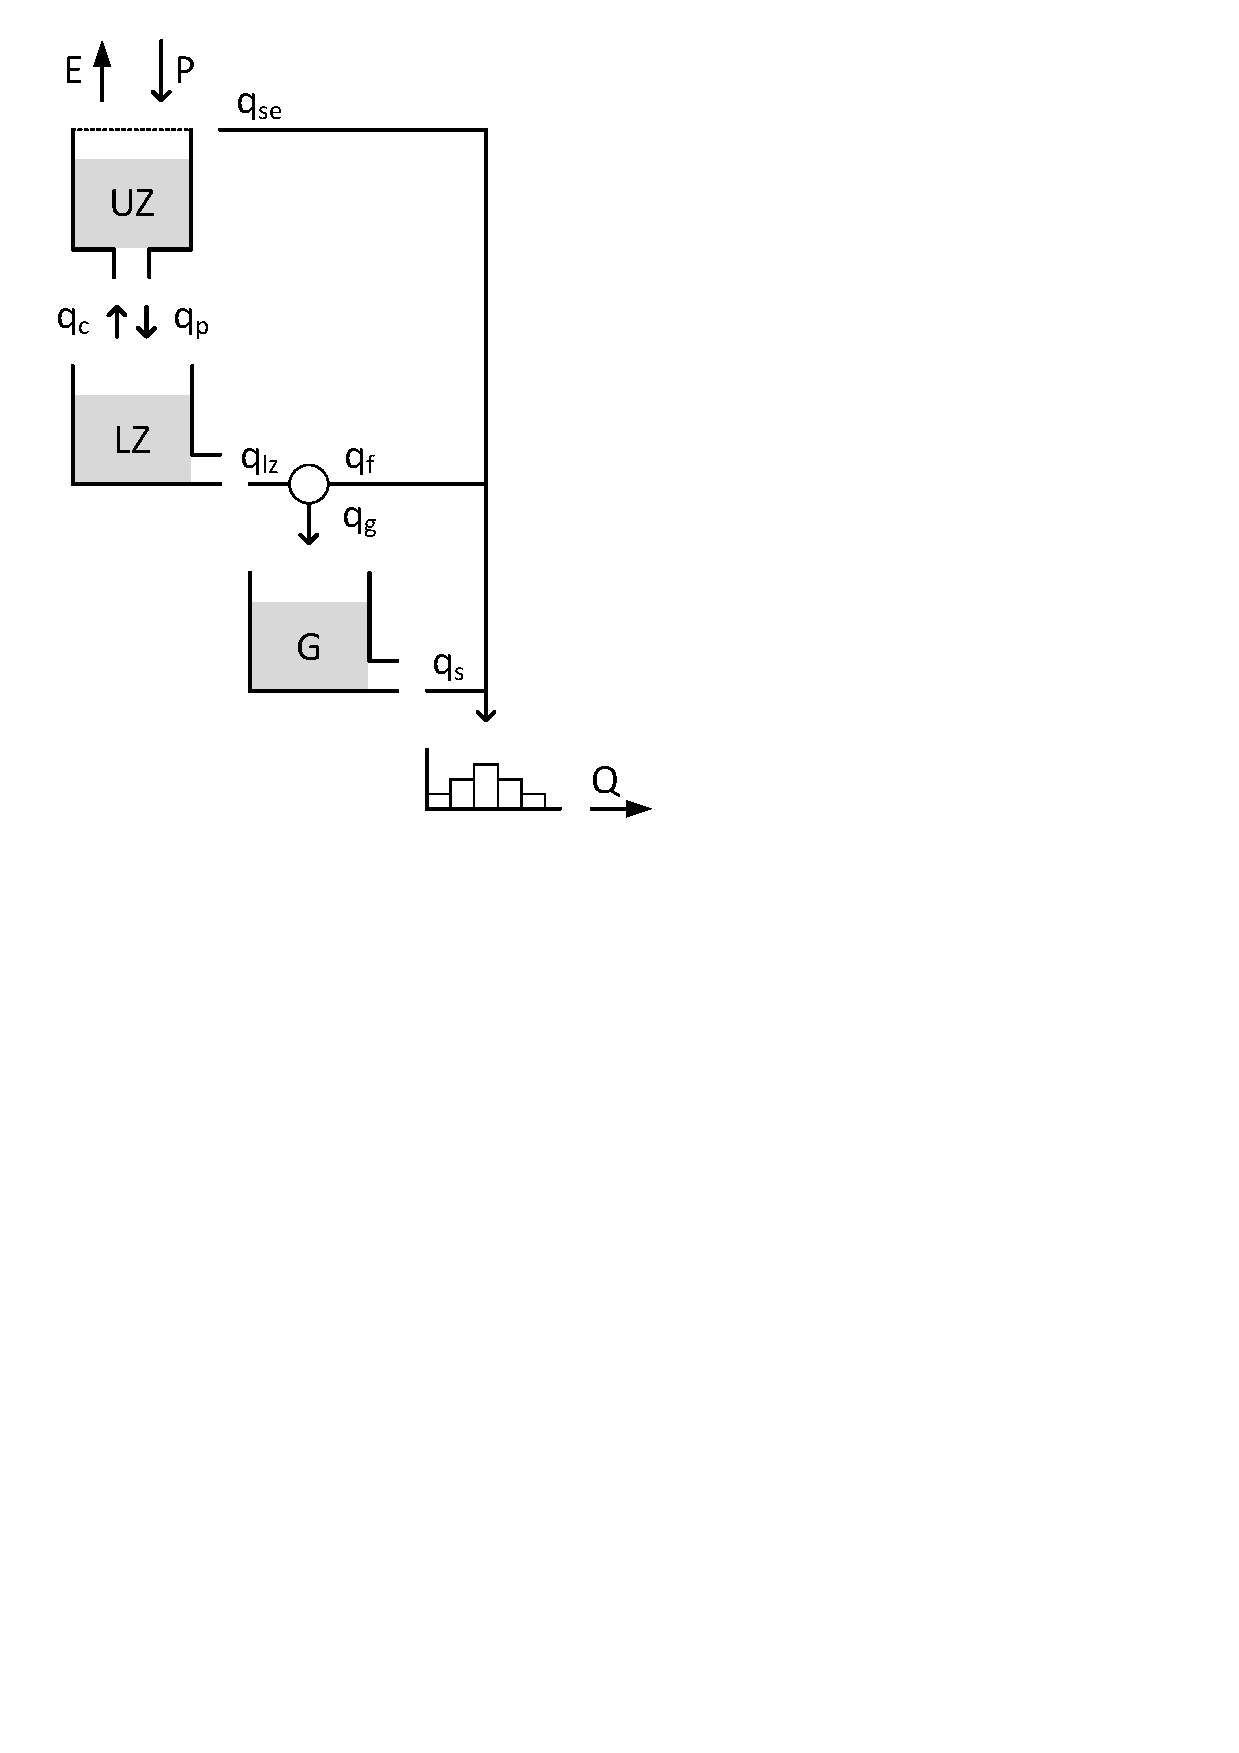
\includegraphics[trim=1cm 16cm 7cm 1cm,width=7cm,keepaspectratio]{./AppA_files/nn_schematic.pdf}
\caption{Structure of the Example model} \label{fig:nn_schematic}
\end{wrapfigure}

\begin{align}
	\frac{dUZ}{dt} &= P+ q_c -E-q_{se}-q_p \\
	E &= E_p*\frac{UZ}{UZ_{max}}\\
	q_c &= c_{rate}\left(1-\frac{UZ}{UZ_{max}}\right)\\
	q_{se} &= \begin{cases}
		P, &\text{if } UZ = UZ_{max}\\
		0, &\text{otherwise}\\
	\end{cases}	\\
	q_p &= p_{rate}
\end{align}

Where $UZ$ [mm] is the current storage in the upper zone, refilled by precipitation $P$ $[mm/d]$ and capillary rise $q_c$ $[mm/d]$ and drained by evaporation $E$ $[mm/d]$, percolation $q_p$ $[mm/d]$ and saturation excess $q_{se}$ $[mm/d]$.
Evaporation occurs at the potential rate $E_p$ scaled by the current storage in $UZ$ compared to maximum storage $UZ_{max}$ [mm].
Capillary rise occurs at a maximum rate $c_{rate}$ $[mm/d]$ if $UZ=0$ and decreases linearly if not.
Saturation excess flow only occurs when $UZ$ is at maximum capacity.
Percolation occurs at a constant rate $p_{rate}$ $[mm/d]$.

} % end of wrapfigure fix

\begin{align}
	\frac{dLZ}{dt} &= q_p - q_c - q_{lz}\\
	q_{lz} &= k_{lz}*LZ 
\end{align}

Where $LZ$ [mm] is the current storage in the lower zone, refilled by percolation $q_p$ $[mm/d]$ and drained by capillary rise $q_c$ $[mm/d]$ and outflow $q_{lz}$ $[mm/d]$.
Outflow has a linear relation with storage through time parameter $k_{lz}$ $[d^{-1}]$.

\begin{align}
	\frac{dG}{dt} &= q_g-q_s\\
	q_g &= \alpha*q_{lz} \\
	q_s &= k_g*G
\end{align}
  
Where $G$ [mm] is the current groundwater storage, refilled by recharge $q_g$ $[mm/d]$ and drained by slow flow $q_s$ $[mm/d]$.
Recharge is a fraction $\alpha$ [-] of outflow from the lower zone.
Outflow has a linear relation with storage through time parameter $k_{g}$ $[d^{-1}]$.
Saturation excess $q_{se}$, interflow $q_f$ and slow flow $q_s$ are combined and routed with a triangular Unit Hydrograph with time base $d$ [d] to give outflow $Q$ $[mm/d]$.

% Parameters
\subsection*{Parameter overview}
% Table generated by Excel2LaTeX from sheet 'Sheet1'
\begin{table}[htbp]
  \centering

    \begin{tabular}{lll}
    \toprule
    Parameter & Unit  & Description \\
    \midrule
    $UZ_{max}$ & $mm$    & Maximum soil moisture storage \\
    $c_{rate}$ & $mm~d^{-1}$ & Capillary rise rate \\
    $p_{rate}$ & $mm~d^{-1}$ & Percolation rate \\
    $k_{lz}$ & $d^{-1}$ & Lower zone runoff coefficient \\
    $\alpha$ & $-$     & Fraction of lower zone runoff that becomes recharge \\
    $k_g$   & $d^{-1}$ & Groundwater runoff coefficient \\
    $d$     & $d$     & Unit Hydrograph time base \\
    \bottomrule
    \end{tabular}%
  \label{tab:addlabel}%
\end{table}%



% Insert all model descriptions
\subsection{Collie River Basin 1 (model ID: 01)}
The Collie River Basin 1 model (fig.~\ref{fig:01_schematic}) is part of a top-down modelling exercise and is originally applied at the annual scale \citep{Jothityangkoon2001}. This is a classic bucket model. It has 1 store and 1 parameter ($S_{max}$). The model aims to represent:

\begin{itemizecompact}
\item Evaporation from soil moisture;
\item Saturation excess surface runoff.
\end{itemizecompact}

\subsubsection{File names}
\begin{tabular}{@{}ll}
Model: &m\_01\_collie1\_1p\_1s \\
Parameter ranges: &m\_01\_collie1\_1p\_1s\_parameter\_ ranges \\
\end{tabular}


% Equations
\subsubsection{Model equations}

% Model layout figure
{ 																	% This ensures it doesn't warp text further down
\begin{wrapfigure}{l}{4.5cm}
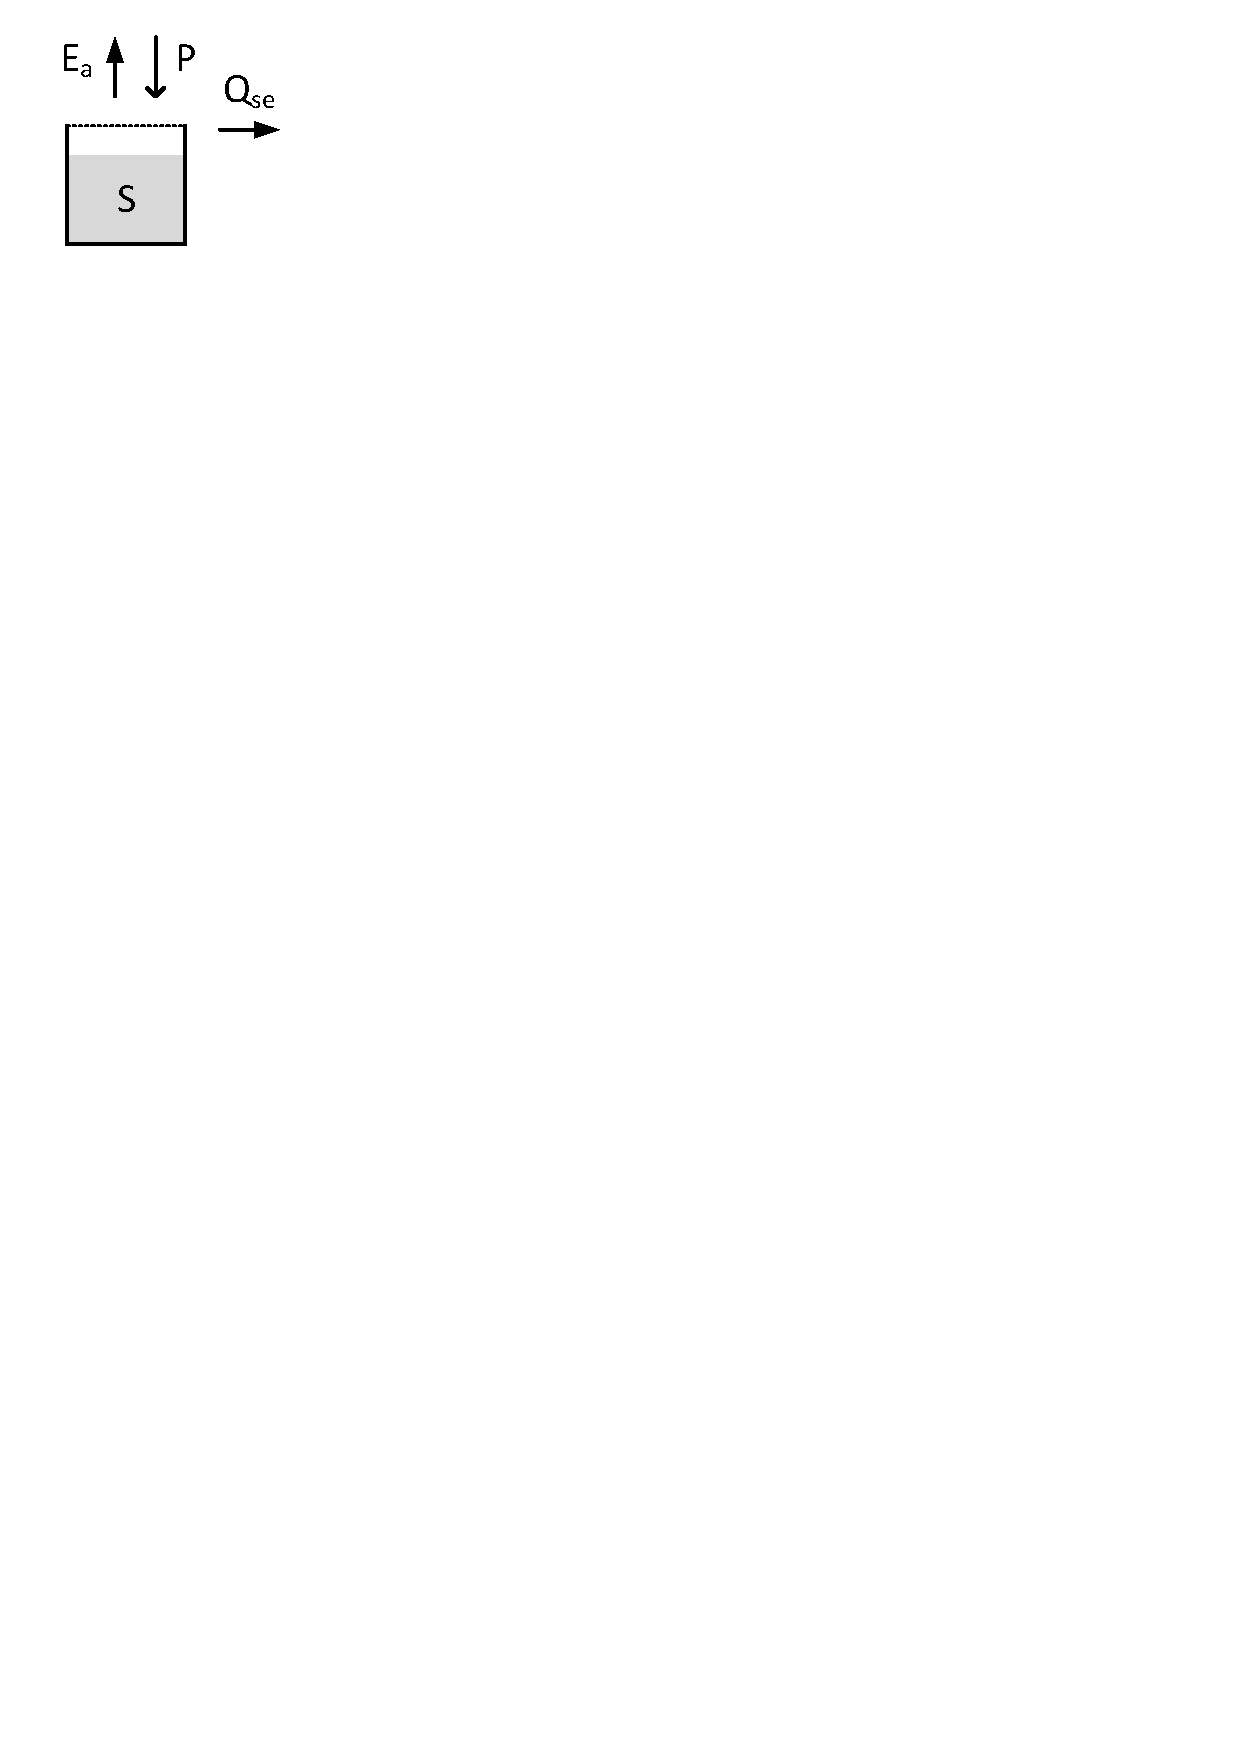
\includegraphics[trim=1cm 25.5cm 9cm 1cm,keepaspectratio]{./files/01_schematic.pdf}
\caption{Structure of the Collie River Basin 1 model} \label{fig:01_schematic}
\end{wrapfigure}

\begin{align}
	\frac{dS}{dt} &= P -E_a-Q_{se} \\
	Ea &= \frac{S}{S_{max}}*Ep\\
	Q_{se} &= 
		\begin{cases}
			P, & if~S>S_{max}\\
			0, & otherwise
		\end{cases}
\end{align}
}
\vspace{1.5cm}

Where  $S$ [mm] is the current storage in the soil moisture and $P$ the precipitation input $[mm/d]$. Actual evaporation $E_a$ $[mm/d]$ is estimated based on the current storage $S$, the maximum soil moisture storage $S_{max}$ [mm], and the potential evapotranspiration $E_p$ $[mm/d]$. $Q_{se}$ $[mm/d]$ is saturation excess overland flow.

\subsubsection{Parameter overview}
% Table generated by Excel2LaTeX from sheet 'Sheet1'
\begin{table}[htbp]
\centering
    \begin{tabular}{lll}
    \toprule
    Parameter & Unit  & Description \\
    \midrule
    $S_{max}$ & $mm$  & Maximum soil moisture storage \\
    \bottomrule
    \end{tabular}%
  \label{tab:addlabel}%
\end{table}%



\subsection{Wetland model (model ID: 02)}
The Wetland model (fig.~\ref{fig:02_schematic}) is a conceptualization of the perceived dominant processes in a typical Western European wetland \citep{Savenije2010}. It belongs to a 3-part topography driven modelling exercise, together with a hillslope and plateau conceptualization. Each model is provided in isolation here, because they are well-suited for isolating specific model structure choices. It has 1 store and 4 parameters ($D_w$, $S_{w,max}$, $\beta_w$ and $K_w$). The model aims to represent:

\begin{itemizecompact}
\item Stylized interception by vegetation;
\item Evaporation;
\item Saturation excess runoff generated from a distribution of soil depths;
\item A linear relation between storage and slow runoff.
\end{itemizecompact}

\subsubsection{File names}
\begin{tabular}{@{}ll}
Model: &m\_02\_wetland\_4p\_1s \\
Parameter ranges: &m\_02\_wetland\_4p\_1s\_parameter\_ ranges \\
\end{tabular}

% Equations
\subsubsection{Model equations}

% Model layout figure
{ 																	% This ensures it doesn't warp text further down
\begin{wrapfigure}{l}{4cm}
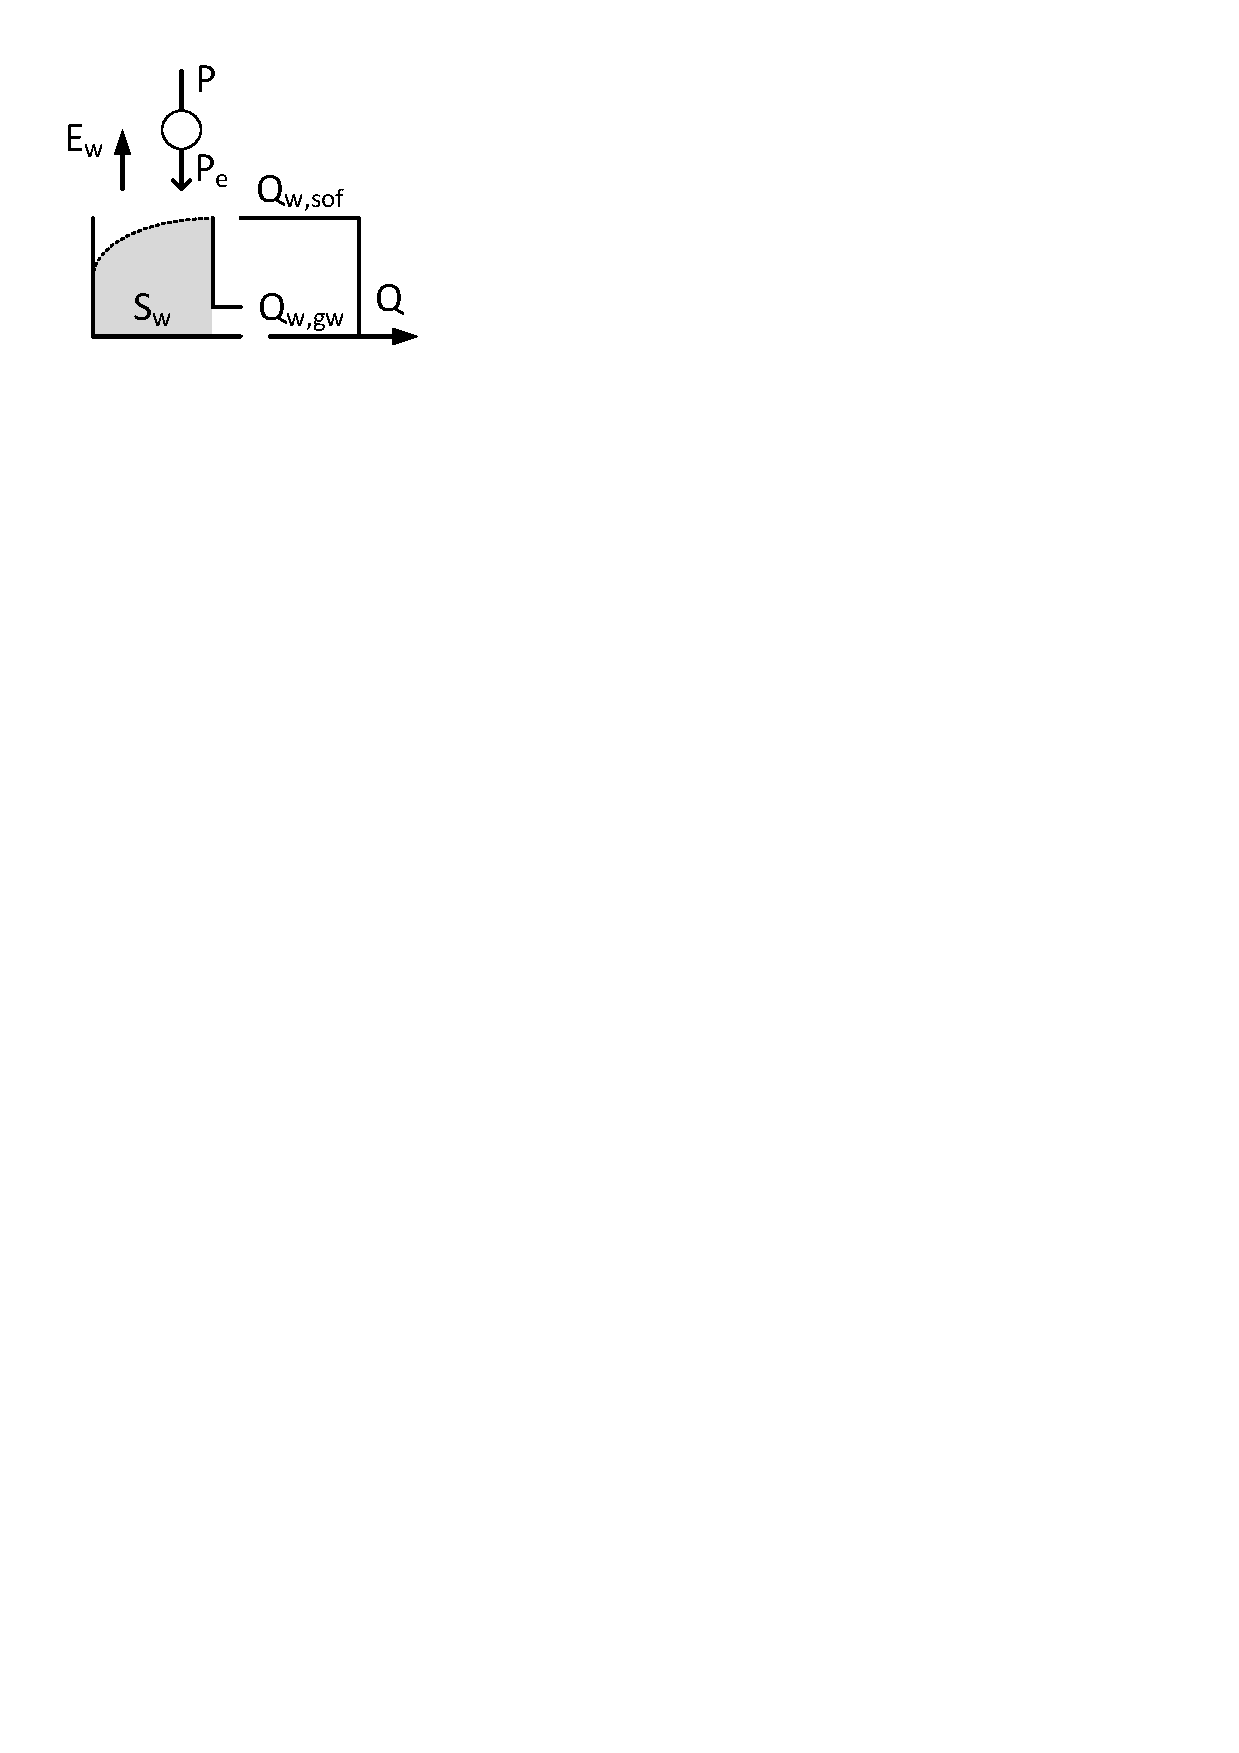
\includegraphics[trim=1cm 24cm 9cm 1cm,width=7cm,keepaspectratio]{./files/02_schematic.pdf}
\caption{Structure of the Wetland model} \label{fig:02_schematic}
\end{wrapfigure}

\begin{align}
	\frac{dS_w}{dt} &= P_e-E_w-Q_{w,sof}-Q_{w,gw} \\
	P_e &= max(P-D_w,0)\\
	E_w &= 
	\begin{cases}
		E_p, & \text{if } S_w > 0 \\
		0, & \text{otherwise}\\
	\end{cases}\\
	Q_{w,sof} &= \left(1-\left(1-\frac{S_w}{S_{w,max}}\right)^{\beta_w}\right)*P_e\\
	Q_{w,gw} &= K_w * S_w
\end{align}

} % end of wrapfigure fix

Where $S_w$ is the current soil water storage [mm]. Incoming precipitation P [mm/d] is reduced by interception $D_w$ [mm/d], which is assumed to evaporate before the next precipitation event. Evaporation from soil moisture $E_w$ [mm/d] occurs at the potential rate $E_p$ whenever possible. Saturation excess surface runoff $Q_{w,sof}$ [mm/d] depends on the fraction of the catchment that is currently saturated, expressed through parameters $S_{w,max}$ [mm] and $\beta_w$ [-]. Groundwater flow $Q_{w,gw}$ [mm/d] depends linearly on current storage $S_w$ through parameter $K_w$ [$d^{-1}$]. Total flow:

\begin{align}
	Q &= Q_{w,sof}+Q_{w,gw}
\end{align}

\newpage
\subsubsection{Parameter overview}
% Table generated by Excel2LaTeX from sheet 'Sheet1'
\begin{table}[htbp]
  \centering
    \begin{tabular}{lll}
    \toprule
    Parameter & Unit  & Description \\
    \midrule
    $D_w$ & $mm~d^{-1}$ & Interception evaporation  \\
    $S_{w,max}$ & $mm$  & Maximum soil moisture storage \\
    $\beta_w$ & $-$   & Non-linearity parameter for contributing area \\
    $K_w$ & $d^{-1}$ & Runoff coefficient \\
    \bottomrule
    \end{tabular}%
  \label{tab:addlabel}%
\end{table}%

\subsection{Collie River Basin 2 (model ID: 03)}
The Collie River Basin 2 model (fig.~\ref{fig:03_schematic}) is part of a top-down modelling exercise and is originally applied at the monthly scale \citep{Jothityangkoon2001}. It has 1 store and 4 parameters ($S_{max}$, $S_{fc}$, $a$, $M$). The model aims to represent:

\begin{itemizecompact}
\item Separate bare soil and vegetation evaporation;
\item Saturation excess surface runoff;
\item Subsurface runoff.
\end{itemizecompact}

\subsubsection{File names}
\begin{tabular}{@{}ll}
Model: &m\_03\_collie2\_4p\_1s \\
Parameter ranges: &m\_03\_collie2\_4p\_1s\_parameter\_ ranges \\
\end{tabular}

% Equations
\subsubsection{Model equations}

% Model layout figure
{ 																	% This ensures it doesn't warp text further down
\begin{wrapfigure}{l}{5cm}
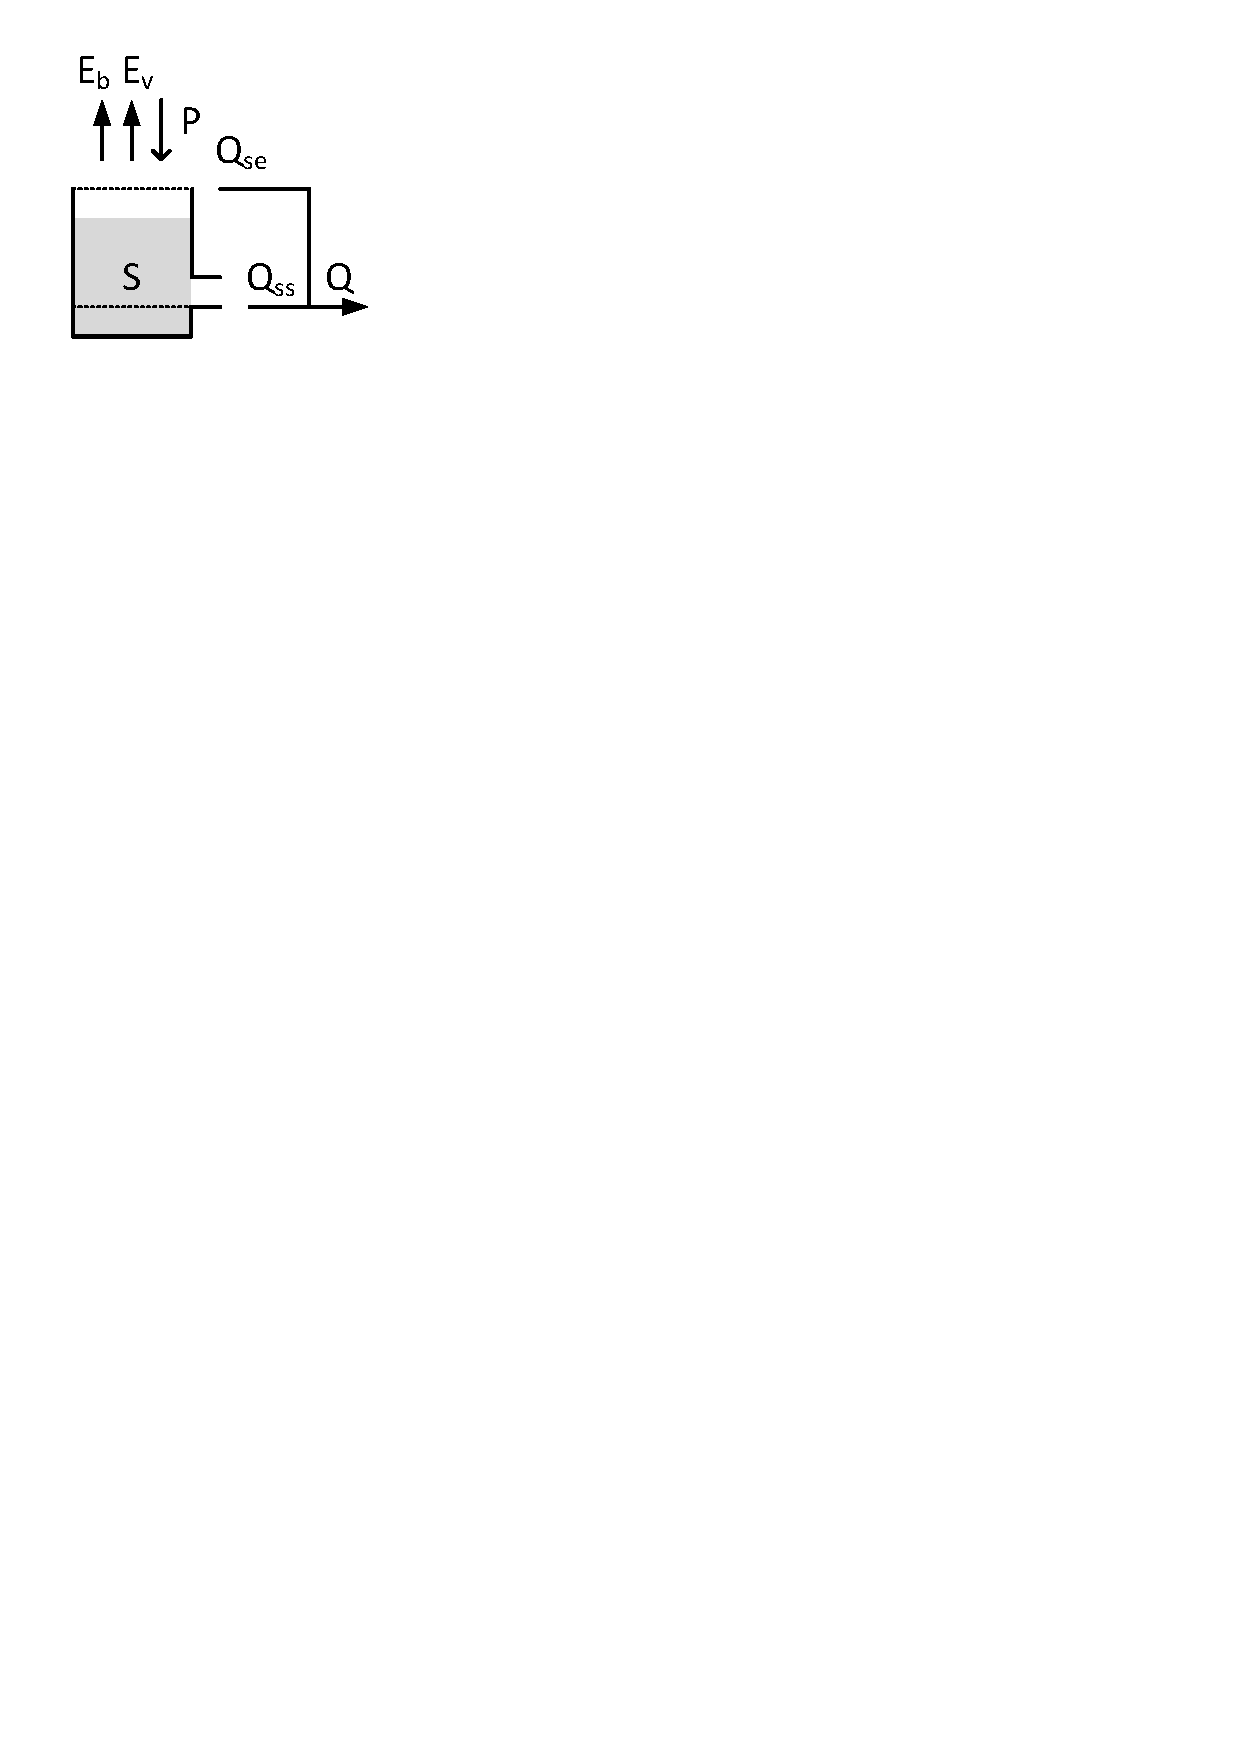
\includegraphics[trim=1cm 24cm 9cm 1cm,keepaspectratio]{./files/03_schematic.pdf}
\caption{Structure of the Collie River Basin 2 model} \label{fig:03_schematic}
\end{wrapfigure}

\begin{align}
	\frac{dS}{dt} &= P -E_b - E_v -Q_{se}-Q_{ss} \\
	Eb &= \frac{S}{S_{max}}(1-M)*Ep\\
	Ev &= 
		\begin{cases}
			M*E_p, & if~S>S_{fc}\\
			\frac{S}{S_{fc}}*M*E_p, &otherwise\\
		\end{cases}\\
	Q_{se} &= 
		\begin{cases}
			P, & if~S>S_{max}\\
			0, & otherwise \\
		\end{cases}\\
	Q_{ss} &= 
		\begin{cases}
			a*(S-S{fc}), & if~S>S_{fc}\\
			0, & otherwise 
		\end{cases}
\end{align}
}
\vspace{0.5cm}

Where $S$ [mm] is the current storage in the soil moisture and $P$ $[mm/d]$ the precipitation input. 
Actual evaporation is split between bare soil evaporation $E_b$ $[mm/d]$ and transpiration through vegetation $E_v$ $[mm/d]$, controlled through the forest fraction $M$ [-]. 
The evaporation estimates are based on the current storage $S$, the potential evapotranspiration $E_p$ $[mm/d]$, maximum soil moisture storage $S_{max}$ [mm] and field capacity $S_{fc}$ [mm] respectively. 
$Q_{se}$ $[mm/d]$ is saturation excess overland flow.  $Q_{ss}$ $[mm/d]$ is subsurface flow regulated by runoff coefficient $a$ $[d^{-1}]$.
Total flow:

\begin{align}
	Q &= Q_{se}+Q_{ss}
\end{align}

\newpage
\subsubsection{Parameter overview}
% Table generated by Excel2LaTeX from sheet 'Sheet1'
\begin{table}[htbp]
  \centering
    \begin{tabular}{lll}
    \toprule
    Parameter & Unit  & Description \\
    \midrule
    $S_{max}$ & $mm$  & Maximum soil moisture storage \\
    $S_{fc}$ & $mm$  & Field capacity \\
    $a$   & $d^{-1}$ & Runoff coefficient \\
    $M$   & $-$   & Forest fraction \\
    \bottomrule
    \end{tabular}%
  \label{tab:addlabel}%
\end{table}%

\include{./files/04_newzealand1}
\subsection{IHACRES (model ID: 05)}
The IHACRES model (fig.~\ref{fig:05_schematic}) as implemented here is a modification of the original equations \citep{Littlewood1997,Ye1997,Croke2004}, which explicitly account for the various fluxes in a step-wise order. 
Furthermore, IHACRES usually uses temperature as a proxy for potential evapotranspiration ($E_p$). 
Here it  uses estimated $E_p$ directly to be consistent with other models. 
The equations for $E_a$ and $U$ are set up following \citet{Croke2004}, with the non-linearity in $U$ based on \citet{Ye1997}. 
This version thus uses a catchment moisture deficit formulation, rather than a catchment wetness index.
\citet{Littlewood1997} recommend the two parallel routing functions. 
The model has 1 \emph{deficit} store and 7 parameters ($lp$, $d$, $p$, $\alpha$, $\tau_q$, $\tau_s$, $\tau_d$). 
The model aims to represent:

\begin{itemizecompact}
\item Catchment deficit build-up
\item Slow and fast routing of effective precipitation.
\end{itemizecompact}

\subsubsection{File names}
\begin{tabular}{@{}ll}
Model: &m\_05\_ihacres\_7p\_1s \\
Parameter ranges: &m\_05\_ihacres\_7p\_1s\_parameter\_ ranges \\
\end{tabular}

% Equations
\subsubsection{Model equations}

% Model layout figure
{ 																	% This ensures it doesn't warp text further down
\begin{wrapfigure}{l}{5cm}
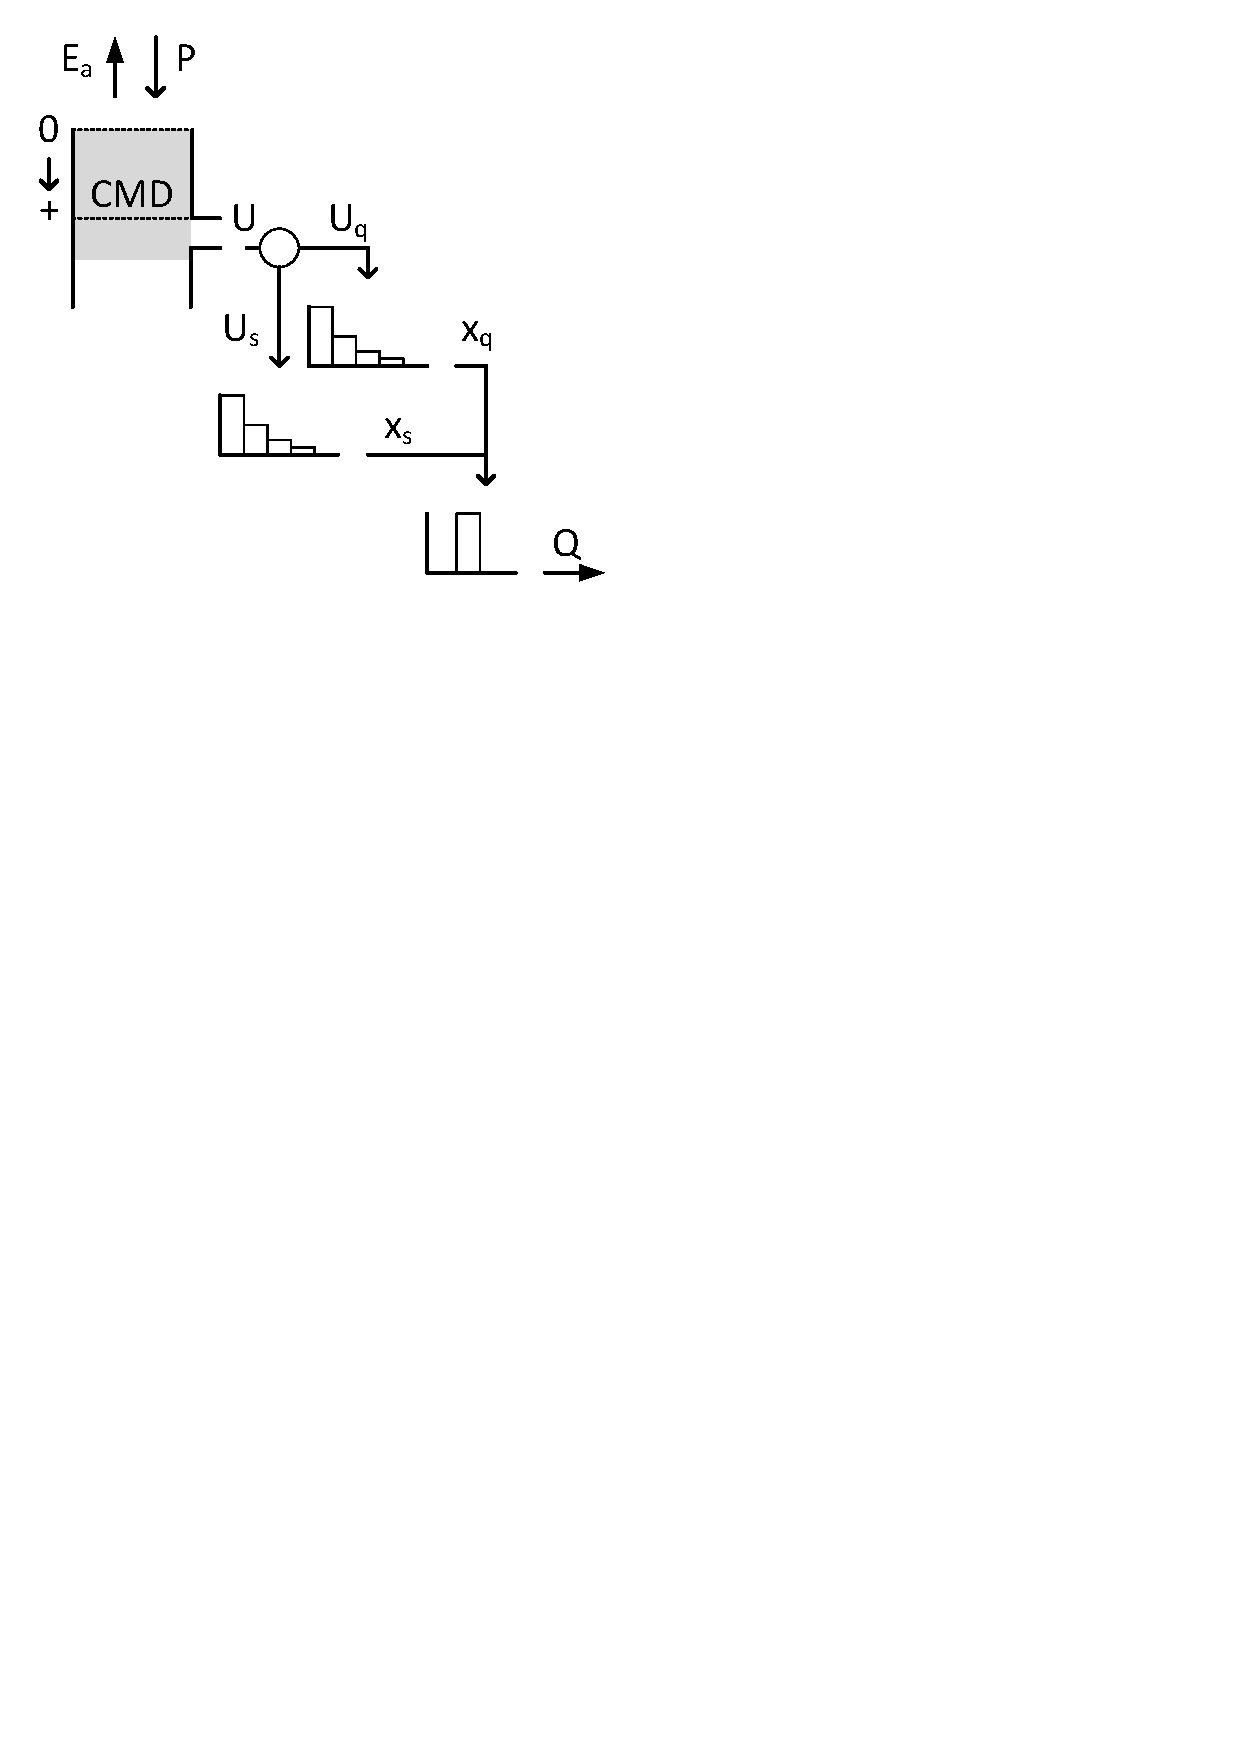
\includegraphics[trim=1cm 20cm 7cm 1cm,width=7cm,keepaspectratio]{./files/05_schematic.pdf}
\caption{Structure of the IHACRES model} \label{fig:05_schematic}
\end{wrapfigure}

\begin{align}
	\frac{dCMD}{dt} &= -P+E_a+U \\
	E_a &= E_p *min\left(1,e^{2\left(1-\frac{CMD}{lp}\right)}\right) \\
	U &= P\left(1-min\left(1,\left(\frac{CMD}{d}\right)^p\right)\right) \\
	U_q &= \alpha *U\\
	U_s &= (1-\alpha)*U
\end{align}

Where $CMD$ is the current moisture deficit [mm], $P$ $[mm/d]$ the incoming precipitation that \emph{reduces} the deficit, $E_a$ $[mm/d]$ evaporation that \emph{increases} the deficit, and $U$ $[mm/d]$ the effective precipitation that occurs when the deficit is below a threshold $d$ [mm], partly controlled by non-linearity parameter $p$ [-].

}

Evaporation occurs at the potential rate $E_p$ until the moisture deficit reaches wilting point $lp$ [mm], after which evaporation decreases exponentially with increasing deficit. Effective precipitation $U$ equals incoming precipitation $P$ when the deficit is zero, and decreases as a linear fraction of P until moisture deficit is larger than a threshold $d$ [mm], after which precipitation does not contribute to streamflow any longer. $U$ is divided between fast and slow routing components based on fraction $\alpha$ [-]. Both routing schemes are exponentially decreasing over time with lags $\tau_q$ [d] and $\tau_s$ [d] respectively. The total flow is given by:

\begin{align}
	Q &= x_q+x_s
\end{align}

which is optionally delayed with a pure time delay $\tau_d$ [d]. Note that this pure delay is not quite the same as the earlier Unit Hydrographs (specified by time base $\tau_q$ and $\tau_s$). The Unit Hydrographs \emph{transform} flow over a given number of time steps, whereas the delay $\tau_d$ \emph{delays} flow by a given number of time steps.

\subsubsection{Parameter overview}
% Table generated by Excel2LaTeX from sheet 'Sheet1'
\begin{table}[htbp]
  \centering
    \begin{tabular}{lll}
    \toprule
    Parameter & Unit  & Description \\
    \midrule
    $lp$  & $mm$  & Wilting point \\
    $d$   & $mm$  & Deficit threshold for flow from rain \\
    $p$   & $-$   & Deficit non-linearity \\
    $\alpha$ & $-$   & Fraction flow to quick routing \\
    $\tau_q$ & $d$   & Unit Hydrograph time base \\
    $\tau_s$ & $d$   & Unit Hydrograph time base \\
    $\tau_d$ & $d$   & Unit Hydrograph delay \\
    \bottomrule
    \end{tabular}%
  \label{tab:addlabel}%
\end{table}%



\section{Alpine model v1 (model ID: 06)}
The Alpine model v1 model (fig.~\ref{fig:06_schematic}) is part of a top-down modelling exercise and represents a monthly water balance model \citep{Eder2003}. 
It has 2 stores and 4 parameters ($T_t$, $ddf$, $S_{max}$, $t_c$). 
The model aims to represent:

\begin{itemizecompact}
\item Snow accumulation and melt;
\item Saturation excess overland flow;
\item Linear subsurface runoff.
\end{itemizecompact}

\subsection{MARRMoT model name}
m\_06\_alpine1\_4p\_2s \\

% Equations
\subsection{Model equations}

% Model layout figure
{ 																	% This ensures it doesn't warp text further down
\begin{wrapfigure}{l}{7cm}
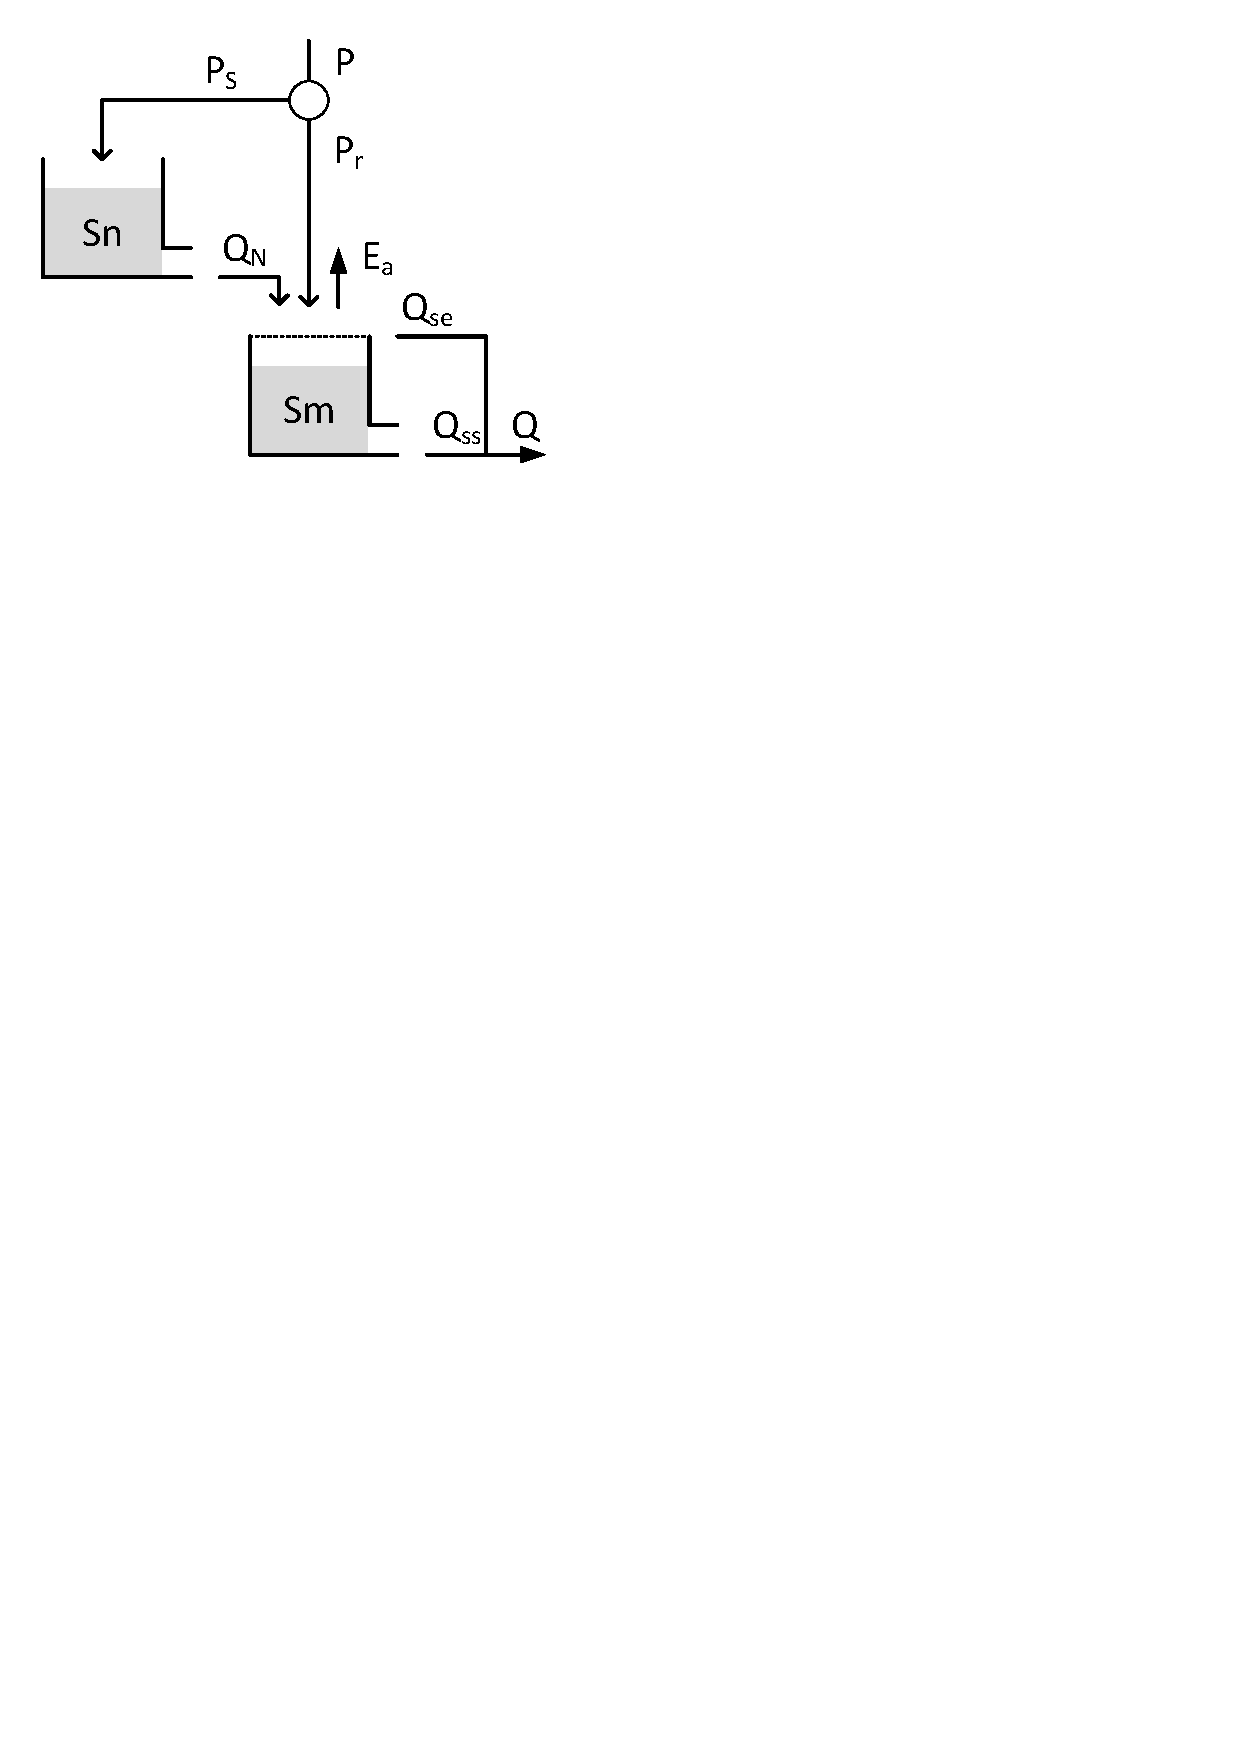
\includegraphics[trim=1cm 22cm 9cm 1cm,width=7cm,keepaspectratio]{./AppA_files/06_schematic.pdf}
\caption{Structure of the Alpine model v1} \label{fig:06_schematic}
\end{wrapfigure}

\begin{align}
	\frac{dSn}{dt} &= P_s-Q_N \\
	P_s &= \begin{cases}
		P, &\text{if } T \leq T_t \\
		0, & \text{otherwise} \\
	\end{cases} \\
	Q_N &= 
	\begin{cases}
		ddf*(T - T_t), & \text{if } T \geq T_t \\
		0, & \text{otherwise}
	\end{cases}
\end{align}

Where $S_N$ is the current snow storage [mm], $P_s$ the precipitation that falls as snow $[mm/d]$, $Q_N$ snow melt $[mm/d]$ based on a degree-day factor (ddf, [mm/\degree C/d]) and threshold temperature for snowfall and snowmelt ($T_t$, [\degree C]).

}

\begin{align}
	\frac{dS_m}{dt} &= P_r + Q_N - E_a  - Q_{se} - Q_{ss}\\
	P_r &= \begin{cases}
		P, &\text{if } T > T_t \\
		0, & \text{otherwise} \\
	\end{cases} \\
	E_a &= \begin{cases}
		E_p, &\text{if } S > 0 \\
		0, &\text{otherwise} \\
	\end{cases} \\
	Q_{se} &= \begin{cases}
		P_r + Q_N, &\text{if } S_m \geq S_{max}\\
		0, &\text{otherwise}\\
	\end{cases}\\
	Q_{ss} &= t_c*S_m	
\end{align}

Where $S_m$ [mm] is the current soil moisture storage, which is assumed to evaporate at the potential rate $E_p$ $[mm/d]$ when possible. When $S_m$ exceeds the maximum storage $S_{max}$ [mm], water leaves the model as saturation excess runoff $Q_{se}$. $Q_{ss}$ represents subsurface flow controlled by time scale parameter $t_c$ $[d^{-1}]$. Total runoff $Q_t$ $[mm/d]$ is:

\begin{equation}
	Q_t = Q_{se} + Q_{ss}
\end{equation}

\subsection{Parameter overview}
% Table generated by Excel2LaTeX from sheet 'Sheet1'
\begin{table}[htbp]
  \centering
    \begin{tabular}{lll}
    \toprule
    Parameter & Unit  & Description \\
    \midrule
    $T_t$ & $^oC$ & Threshold temperature for snowfall and melt \\
    $ddf$ & $mm~^oC^{-1}~d^{-1}$ & Degree-day factor \\
    $S_{max}$ & $mm$  & Maximum soil moisture storage \\
    $t_c$ & $d^{-1}$ & Runoff coefficient \\
    \bottomrule
    \end{tabular}%
  \label{tab:addlabel}%
\end{table}%


\section{GR4J (model ID: 07)}
The GR4J model (fig.~\ref{fig:07_schematic}) is originally developed with an explicit (operator-splitting) time-stepping scheme \citep{Perrin2003}. Recently a new version has been released that works with an implicit time-stepping scheme \citep{Santos2017}. The implementation given here follows most of the equations from \citet{Santos2017}, but uses the original Unit Hydrographs for flood routing given by \citet{Perrin2003}. It has 2 stores and 4 parameters ($x_1$, $x_2$, $x_3$, $x_4$). The model aims to represent:

\begin{itemizecompact}
\item Implicit interception by vegetation, expressed as net precipitation or evaporation;
\item Different time delays within the catchment expressed by two hydrographs;
\item Water exchange with neighbouring catchments.
\end{itemizecompact}

\subsection{MARRMoT model name}
m\_07\_gr4j\_4p\_2s \\

% Equations
\subsection{Model equations}

% Model layout figure
{ 																	% This ensures it doesn't warp text further down
\begin{wrapfigure}{l}{5cm}
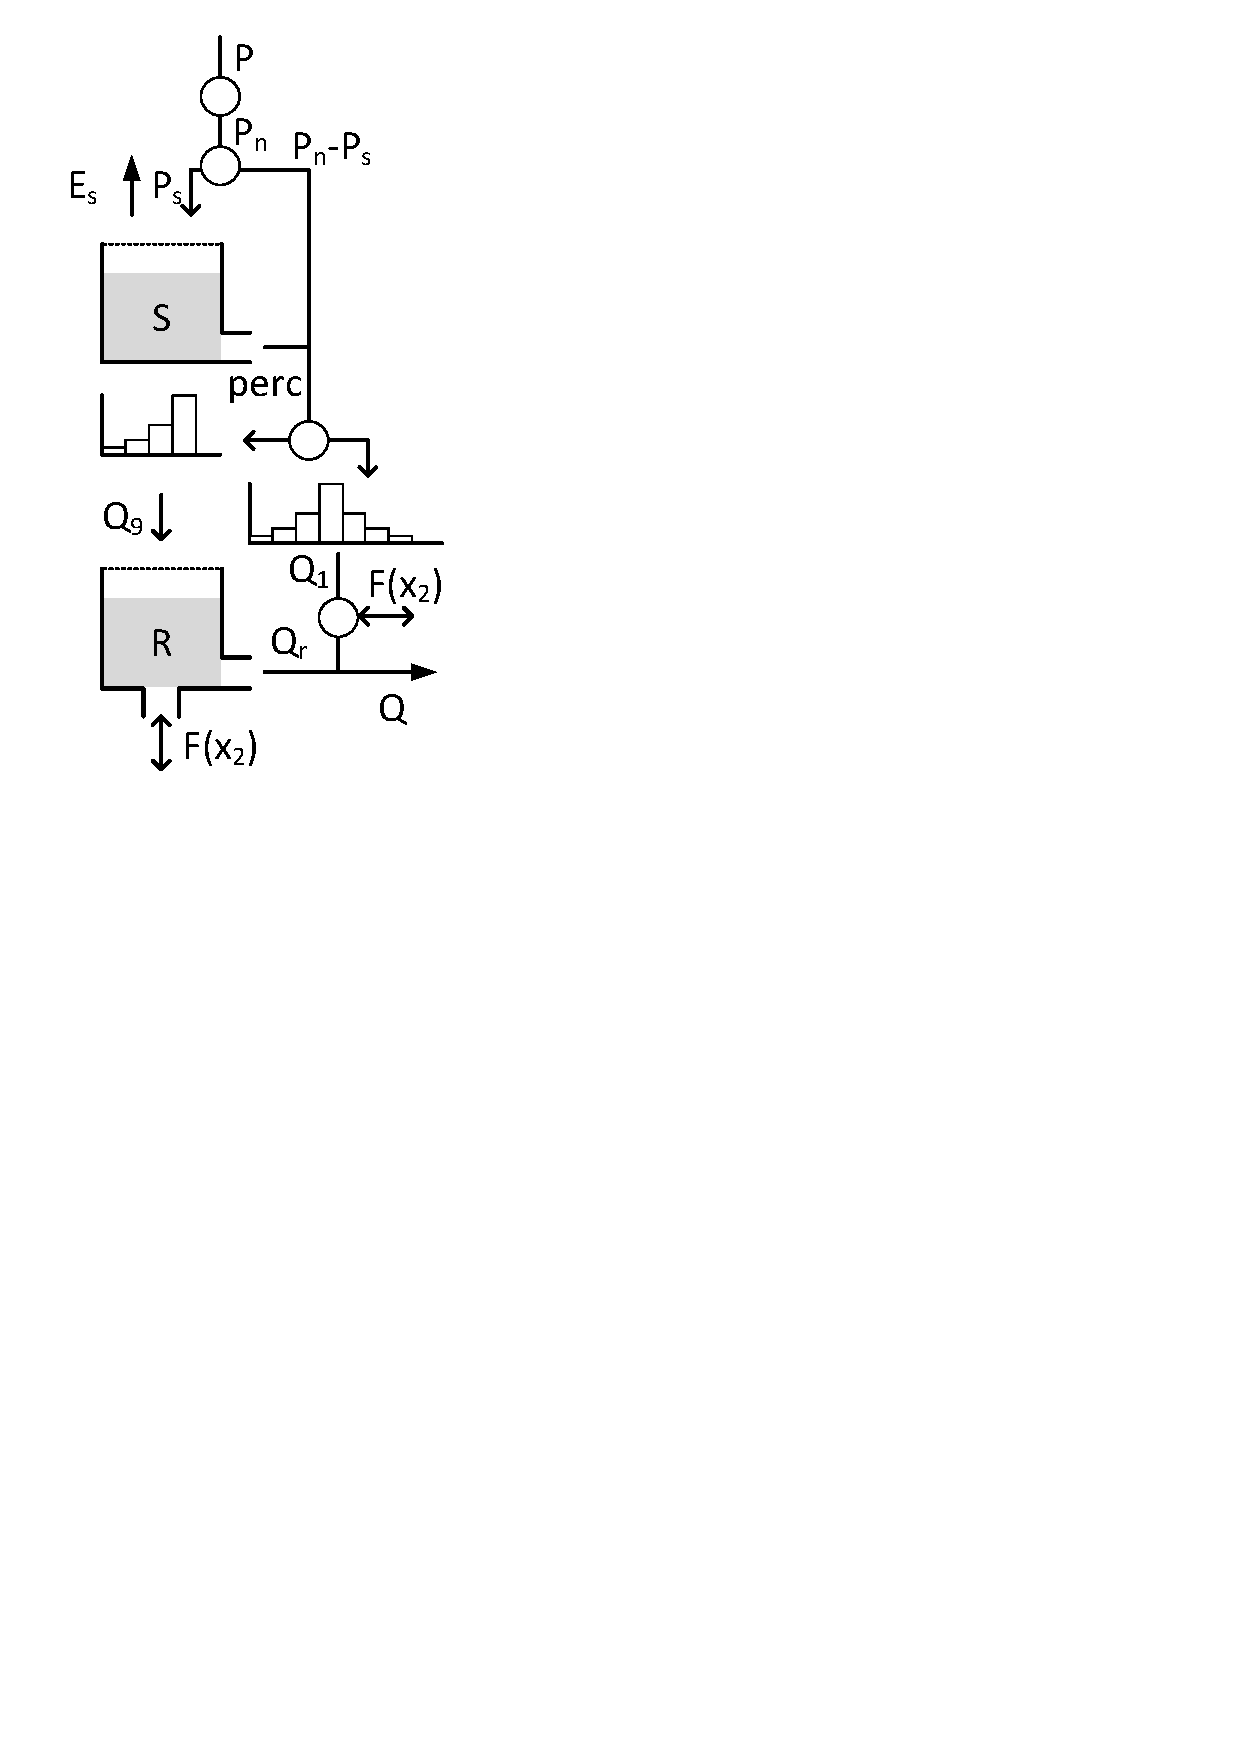
\includegraphics[trim=1cm 17cm 7cm 1cm,width=8cm,keepaspectratio]{./AppA_files/07_schematic.pdf}
\caption{Structure of the GR4J model} \label{fig:07_schematic}
\end{wrapfigure}

\begin{align}
	\frac{dS}{dt} &= P_s-E_s-Perc \\
	P_s &= P_n* \left(1-\left(\frac{S}{x1}\right)^2\right)\\
	P_n &= 
	\begin{cases}
		P-Ep, & \text{if } P \geq Ep \\
		0, & \text{otherwise}
	\end{cases} \\
	E_s &= E_n*\left(2\frac{S}{x1}-\left(\frac{S}{x1}\right)^2\right)\\
	E_n &= 
	\begin{cases}
		Ep-P, & \text{if } Ep > P \\
		0, & \text{otherwise}
	\end{cases} \\
	Perc &= \frac{x_1^{-4}}{4}*\left(\frac{4}{9}\right)^{-4}S^5
\end{align}

Where S is the current soil moisture storage [mm], $P_s$ $[mm/d]$ is the fraction of net precipitation $P_n$ $[mm/d]$ redirected to soil moisture, $E_s$ $[mm/d]$ is the fraction of net evaporation $E_n$ $[mm/d]$ subtracted from soil moisture, and $perc$ $[mm/d]$ is percolation to deeper soil layers. Parameter $x_1$ [mm] is the maximum soil moisture storage.

} % end of wrapfigure fix

Percolation $perc$ and excess precipitation $P_n - P_s$ are divided into 90\% groundwater flow, routed through a triangular routing scheme with time base $x_4$ [d], and 10\% direct runoff, routed through a triangular routing scheme with time base $2x_4$ [d].

\begin{align}
	\frac{dR}{dt} &= Q_{9} + F(x_2) -Q_r\\
	F(x_2) &= x_2*\left(\frac{R}{x_3}\right)^{3.5} \\	
	Q_r &= \frac{x_3^{-4}}{4}R^5
\end{align}

Where $R$ [mm] is the current storage in the routing store, $F(x_2)$ $[mm/d]$ the catchment groundwater exchange, depending on exchange coefficient $x_2$ $[mm/d]$ and the maximum routing capacity $x_3$ [mm], and $Q_r$ $[mm/d]$ routed flow. Total runoff $Q_t$ $[mm/d]$: 

\begin{equation}
	Q_t = Q_r + max(Q_1+F(x_2),0)
\end{equation} 

\subsection{Parameter overview}
% Table generated by Excel2LaTeX from sheet 'Sheet1'
\begin{table}[htbp]
  \centering
    \begin{tabular}{lll}
    \toprule
    Parameter & Unit  & Description \\
    \midrule
    $x_1$ & $mm$  & Maximum soil moisture storage \\
    $x_2$ & $mm~d^{-1}$ & Subsurface water exchange \\
    $x_3$ & $mm$  & Routing store depth \\
    $x_4$ & $d$   & Unit Hydrograph time base \\
    \bottomrule
    \end{tabular}%
  \label{tab:addlabel}%
\end{table}%


\subsection{United States model (model ID: 08)}
The United States model (fig.~\ref{fig:08_schematic}) is part of a multi-model comparison study using several catchments in the United States \citep{Bai2009}. It has 2 stores and 5 parameters ($\alpha_{ei}$, $M$, $S_{max}$, $fc$, $\alpha_{ss}$). The model aims to represent:

\begin{itemizecompact}
\item Interception as a percentage of precipitation;
\item Separate unsaturated and saturated zones;
\item Separate bare soil evaporation and vegetation transpiration;
\item Saturation excess overland flow;
\item Subsurface flow.
\end{itemizecompact}

\subsubsection{File names}
\begin{tabular}{@{}ll}
Model: &m\_08\_us1\_5p\_2s \\
Parameter ranges: &m\_08\_us1\_5p\_2s\_parameter\_ ranges \\
\end{tabular}

% Equations
\subsubsection{Model equations}

% Model layout figure
{ 																	% This ensures it doesn't warp text further down
\begin{wrapfigure}{l}{5cm}
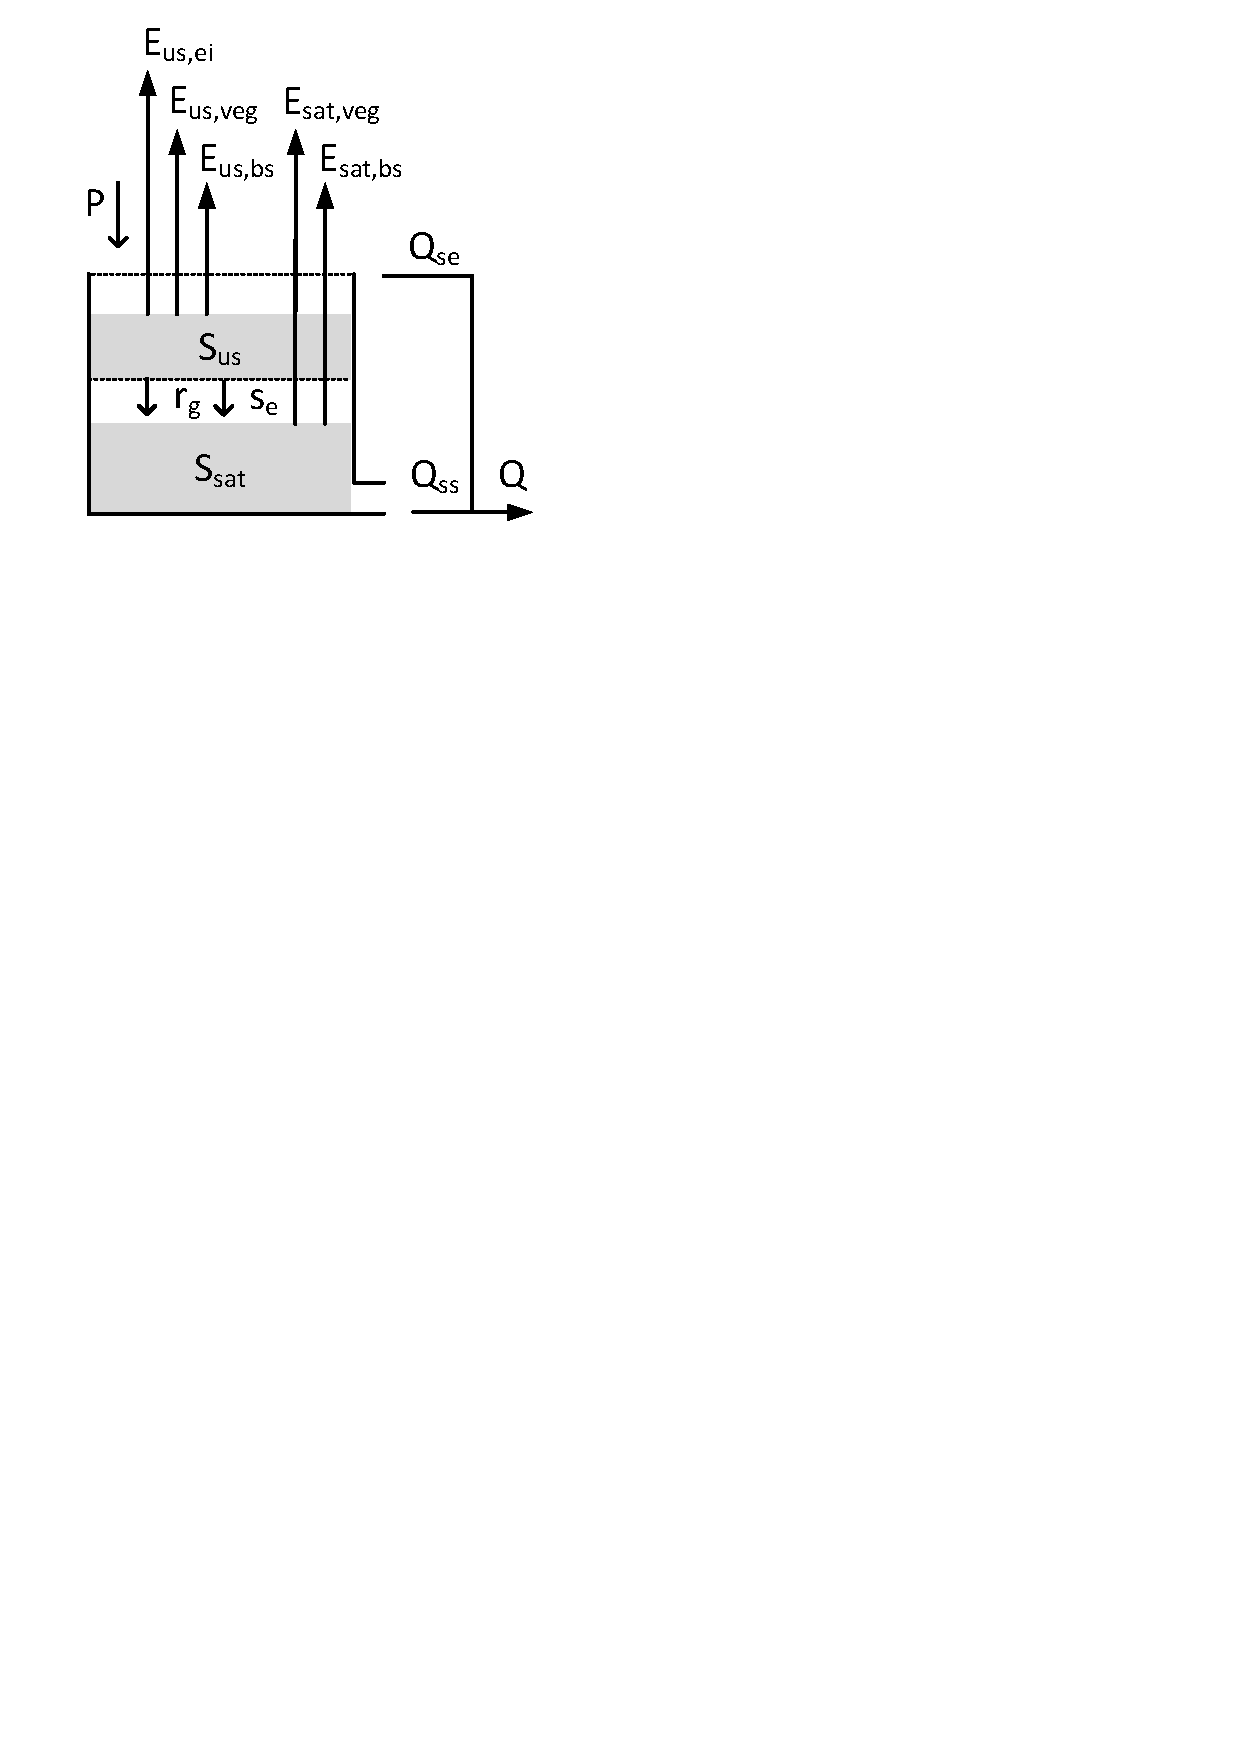
\includegraphics[trim=1cm 21cm 9cm 1cm,width=7cm,keepaspectratio]{./files/08_schematic.pdf}
\caption{Structure of the United States model} \label{fig:08_schematic}
\end{wrapfigure}

\begin{align}
	\frac{dS_{us}}{dt} &= P - E_{us,ei}-E_{us,veg}-E_{us,bs}-r_g \\
	E_{us,ei} &= \alpha_{ei}*P\\
	E_{us,veg} &= \begin{cases}
		\frac{S_{us}}{S_{us}+S_{sat}}*M*E_p, &\text{if } S_{us} > S_{usfc} \\
		\frac{S_{us}}{S_{us}+S_{sat}}*M*E_p*\frac{S_{us}}{S_{usfc}}, & \text{otherwise} \\
	\end{cases} \\
	E_{us,bs} &= \frac{S_{us}}{S_{us}+S_{sat}}*(1-M)*\frac{S_{us}}{S_{max}-S_{sat}}*E_p\\
	r_g &=\begin{cases}
		P, &\text{if } S_{us} > S_{usfc}\\
		0, & \text{otherwise} \\
	\end{cases}\\
	S_e &= \begin{cases}
			S_{us} - S_{usfc}, & if~S_{us} > S_{usfc}\\
			0, & \text{otherwise} \\
			\end{cases}\\
	S_{usfc} &= fc*(S_{max} - S_{sat})
\end{align}
} % end of wrap figure

Where $S_{us}$ [mm] is the current storage in the unsaturated zone, $E_{us,ei}$ $[mm/d]$ evaporation from interception, $E_{us,veg}$ $[mm/d]$ transpiration through vegetation, $E_{us,bs}$ $[mm/d]$ bare soil evaporation and $r_g$ $[mm/d]$ drainage to the saturated zone. Interception evaporation relies on parameter $\alpha_{ei}$ [-], representing the fraction of precipitation P that is intercepted. The implicit assumption is that this evaporates before the next precipitation event. Transpiration uses forest fraction $M$ [-], potential evapotranspiration $E_p$ $[mm/d]$ and the estimated field capacity $S_{usfc}$ through parameter $fc$ [-]. Bare soil evaporation relies also on the maximum soil moisture storage $S_{max}$ [mm]. 

\begin{align}
	\frac{dS_{sat}}{dt} &= r_g - E_{sat,veg}-E_{sat,bs} -Q_{se} - Q_{ss}\\
	E_{sat,veg} &= \frac{S_{sat}}{S_{max}}*M*E_p\\
	E_{sat,bs} &= \frac{S_{sat}}{S_{max}}*(1-M)*E_p\\
	Q_{se} &=\begin{cases}
		r_g, &\text{if } S_{us} \geq S_{max}\\
		0, & \text{otherwise} \\
	\end{cases}\\
	Q_{ss} &= \alpha_{ss}*S_{sat}
\end{align}

Where $S_{sat}$ [mm] is the current storage in the saturated zone, $E_{sat,veg}$ $[mm/d]$ transpiration through vegetation, $E_{sat,bs}$ $[mm/d]$ bare soil evaporation, $Q_{se}$ $[mm/d]$ saturation excess overland flow and $Q_{ss}$ $[mm/d]$ subsurface flow. Subsurface flow uses time parameter $\alpha_{ss}$ $[d^{-1}]$
Total flow:

\begin{align}
	Q &= Q_{se}+Q_{ss}
\end{align}

\subsubsection{Parameter overview}
% Table generated by Excel2LaTeX from sheet 'Sheet1'
\begin{table}[htbp]
  \centering
    \begin{tabular}{lll}
    \toprule
    Parameter & Unit  & Description \\
    \midrule
    $\alpha_{ei}$ & $-$   & Intercepted fraction of precipitation \\
    $M$   & $-$   & Forest fraction \\
    $S_{max}$ & $mm$  & Maximum soil moisture storage \\
    $fc$  & $-$   & Field capacity as fraction of $S_{max}$ \\
    $\alpha_{ss}$ & $d^{-1}$ & Runoff coefficient \\
    \bottomrule
    \end{tabular}%
  \label{tab:addlabel}%
\end{table}%


\subsection{ Susannah Brook model v1-5 (model ID: 09)}
The Susannah Brook model v1-5 (fig.~\ref{fig:09_schematic}) is part of a top-down modelling exercise designed to use auxiliary data \citep{Son2007}. It has 2 stores and 6 parameters ($S_b$, $S_{fc}$, $M$, $a$, $b$ and $r$). The model aims to represent:

\begin{itemizecompact}
\item Evaporation from soil and transpiration from vegetation;
\item Saturation excess and non-linear subsurface flow;
\item Groundwater recharge and baseflow.
\end{itemizecompact}

\subsubsection{File names}
\begin{tabular}{@{}ll}
Model: &m\_09\_susannah1\_6p\_2s \\
Parameter ranges: &m\_09\_susannah1\_6p\_2s\_parameter\_ ranges \\
\end{tabular}

% Equations
\subsubsection{Model equations}

% Model layout figure
{ 																	% This ensures it doesn't warp text further down
\begin{wrapfigure}{l}{5cm}
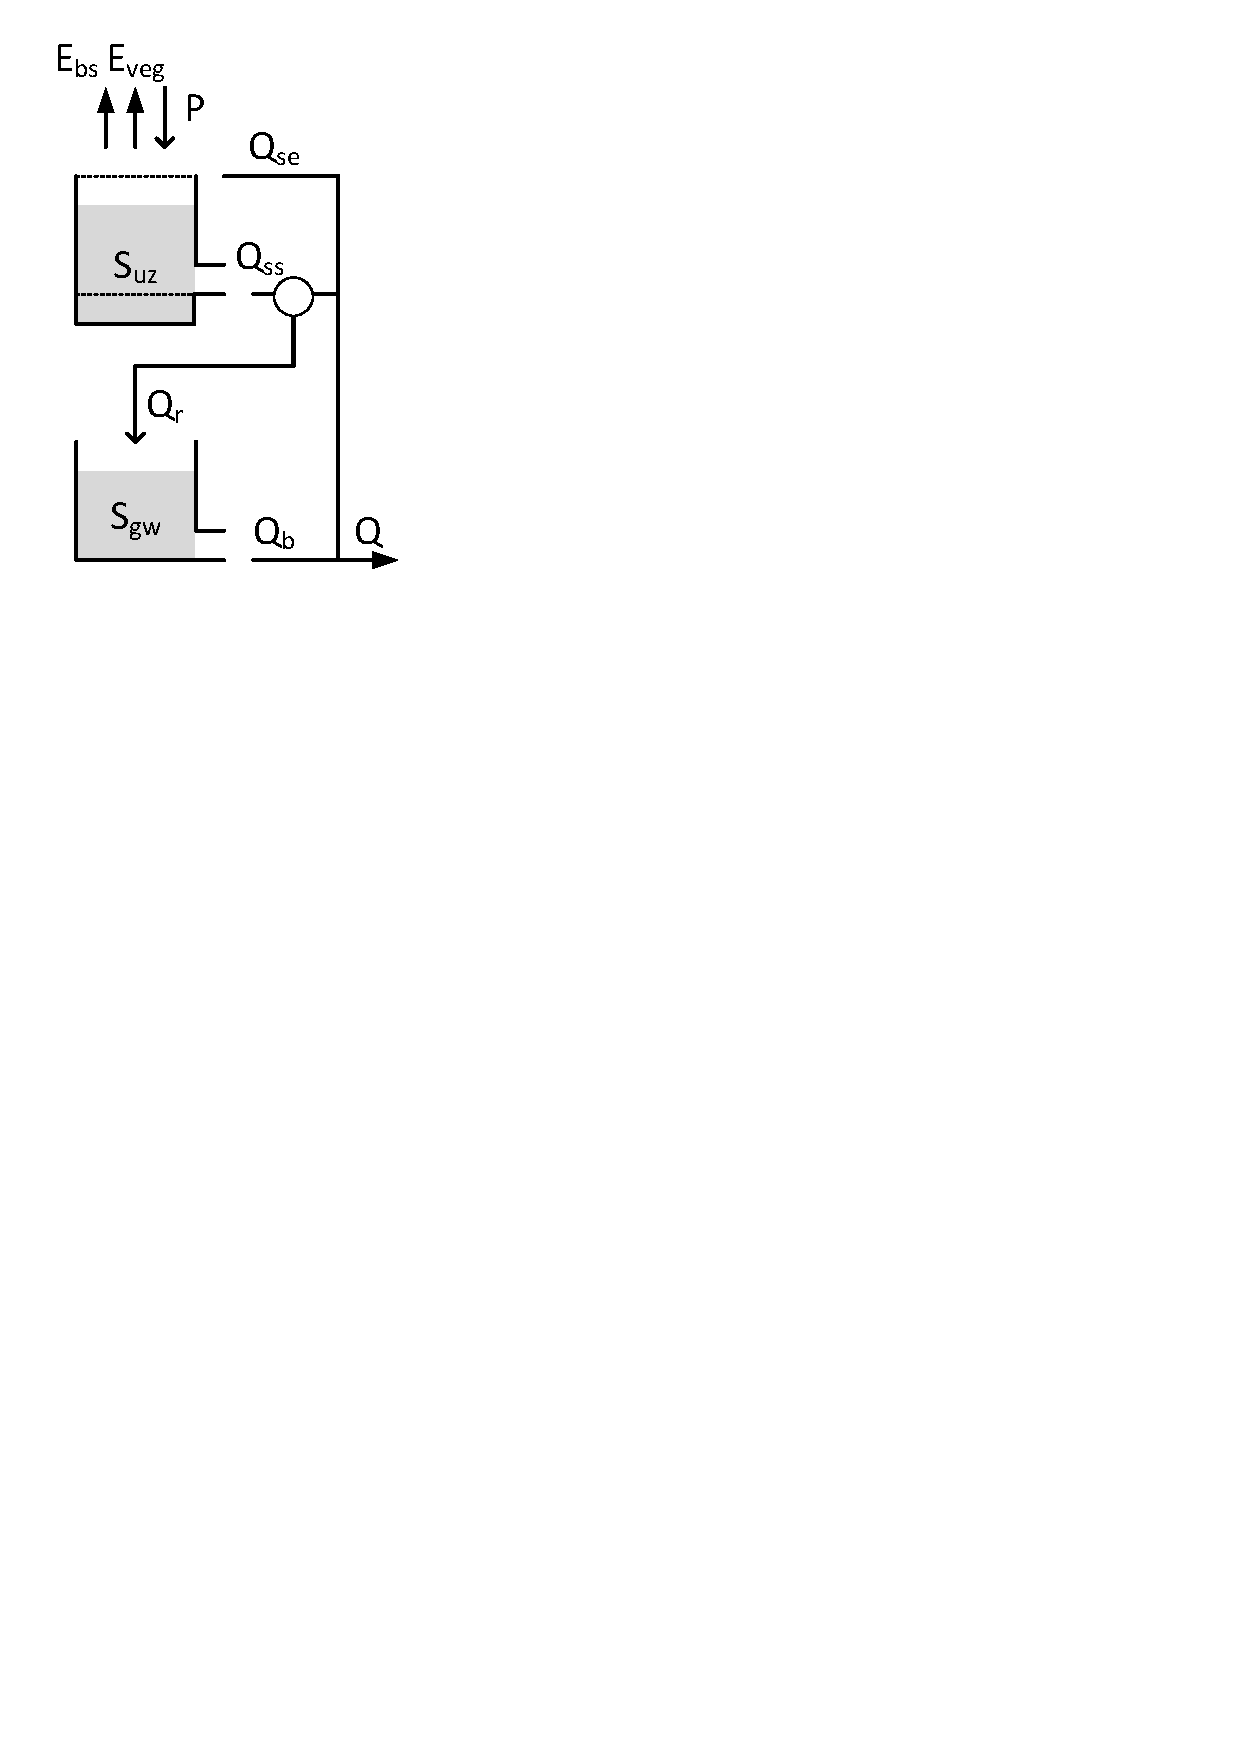
\includegraphics[trim=1cm 20cm 10cm 1cm,width=7cm,keepaspectratio]{./files/09_schematic.pdf}
\caption{Structure of the Susannah Brook model v1-5} \label{fig:09_schematic}
\end{wrapfigure}

\begin{align}
	\frac{dS_{uz}}{dt} &= P-E_{bs}-E_{veg}-Q_{se}-Q_{ss}\\
	E_{bs} &= \frac{S}{S_b}\left(1-M\right)E_p\\
	E_{veg} &= \begin{cases}
		M*E_p, &\text{if } S >S_{fc}\\
		\frac{S}{S_{fc}}M*E_p, &\text{otherwise}\\
	\end{cases}\\
	Q_{se} &= \begin{cases}
		P, &\text{if } S \geq S_b\\
		0, &\text{otherwise}\\
	\end{cases}\\
	Q_{ss} &= \begin{cases}
		\left(\frac{S-S_{fc}}{a}\right)^{\frac{1}{b}}, &\text{if } S > S_{fc}\\
		0, &\text{otherwise}\\
	\end{cases}
\end{align}

\vspace{2cm}
}

Where $S_{uz}$ is current storage in the upper zone [mm]. 
P [mm/d] is the precipitation input. 
$E_{bs}$ is bare soil evaporation [mm/d] based on soil depth 
$S_b$ [mm] and forest fraction $M$ [-]. $E_{veg}$ is transpiration from vegetation, using the wilting point $S_{fc}$ [mm] and forest fraction $M$. $Q_{se}$ is saturation excess flow [mm/d]. 
$Q_{ss}$ is non-linear subsurface flow, using the wilting point $S_{fc}$ [mm] as a threshold for flow generation and two flow parameters $a$ [d] and $b$ [-]. $Q_r$ is groundwater recharge [mm/d].

\begin{align}
	\frac{DS_{gw}}{dt} &= Q_r-Q_b\\
	Q_r &= r*Q_{ss}\\
	Q_b &= \left(\frac{1}{a}S_{gw}\right)^{\frac{1}{b}}
\end{align}	

Where $S_{gw}$ is the groundwater storage [mm], and $Q_b$ the baseflow flux [mm/d]. $r$ is the fraction of subsurface flow $Q_{ss}$ that goes to groundwater. Total flow [mm]:

\begin{align}
	Q &= Q_{se} + (Q_{ss} - Q_r) + Q_b
\end{align}

\subsubsection{Parameter overview}
% Table generated by Excel2LaTeX from sheet 'Sheet1'
\begin{table}[htbp]
  \centering
    \begin{tabular}{lll}
    \toprule
    Parameter & Unit  & Description \\
    \midrule
    $S_b$ & $mm$  & Maximum soil moisture storage \\
    $S_{fc}$ & $mm$  & Field capacity \\
    $M$   & $-$   & Forest fraction \\
    $a$   & $d$   & Runoff time coefficient \\
    $b$   & $-$   & Runoff nonlinearity \\
    $r$   & $-$   & Fraction subsurface flow to groundwater \\
    \bottomrule
    \end{tabular}%
  \label{tab:addlabel}%
\end{table}%



\subsection{Susannah Brook model v2 (model ID: 10)}
The Susannah Brook model v2 model (fig.~\ref{fig:10_schematic}) is part of a top-down modelling exercise designed to use auxiliary data \citep{Son2007}. It has 2 stores and 6 parameters ($S_b$, $\phi$, $fc$, $r$, $c$, $d$). For consistency with other model formulations, $S_b$ is is used as a parameter, instead of being broken down into its constitutive parts $D$ and $\phi$. The model aims to represent:

\begin{itemizecompact}
\item Separation of saturated zone and a variable-size unsaturated zone;
\item Evaporation from unsaturated and saturated zones;
\item Saturation excess and non-linear subsurface flow;
\item Deep groundwater recharge.
\end{itemizecompact}

\subsubsection{File names}
\begin{tabular}{@{}ll}
Model: &m\_10\_susannah2\_6p\_2s \\
Parameter ranges: &m\_10\_susannah2\_6p\_2s\_parameter\_ ranges \\
\end{tabular}

% Equations
\subsubsection{Model equations}

% Model layout figure
{ 																	% This ensures it doesn't warp text further down
\begin{wrapfigure}{l}{5cm}
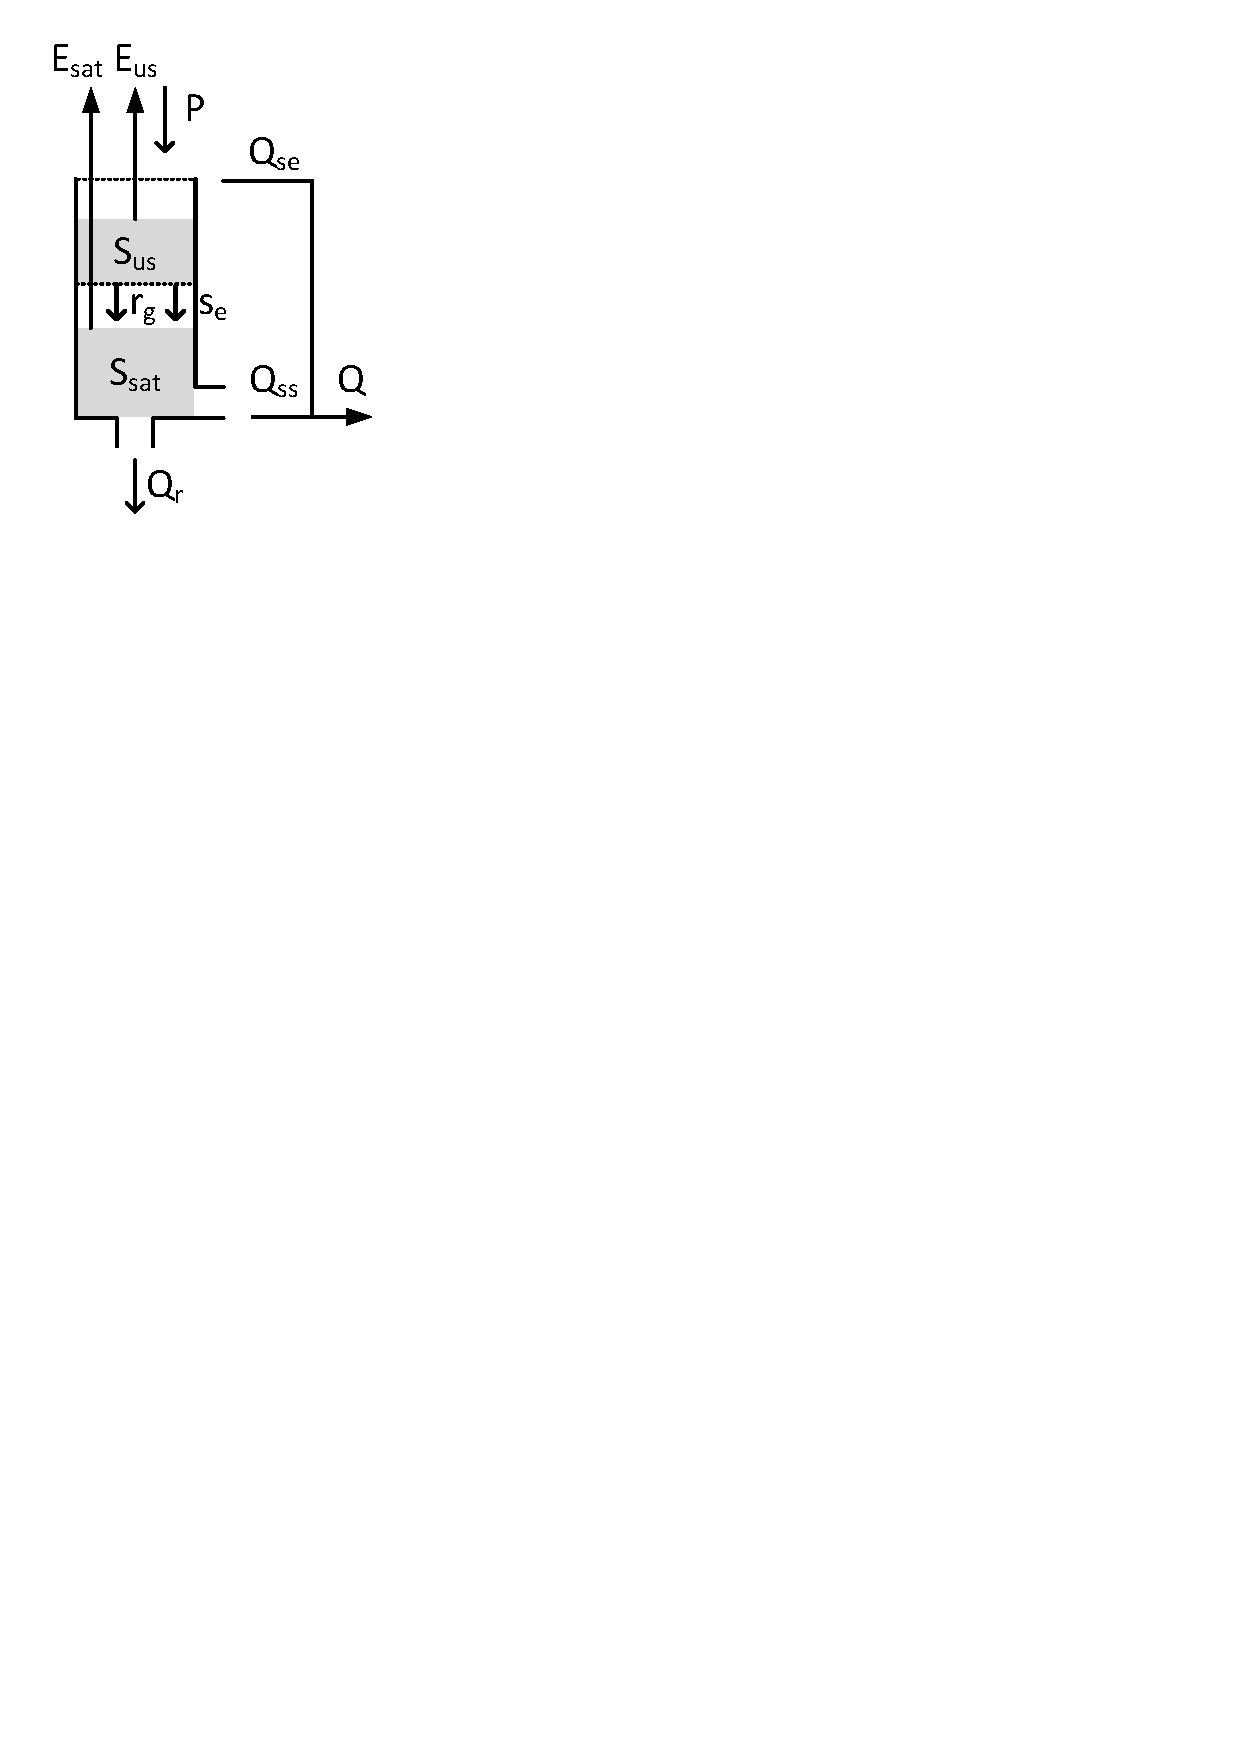
\includegraphics[trim=1cm 21cm 14cm 0.8cm,width=5cm,keepaspectratio]{./files/10_schematic.pdf}
\caption{Structure of the Susannah Brook v2 model} \label{fig:10_schematic}
\end{wrapfigure}

\begin{align}
	\frac{dS_{us}}{dt} &= P-E_{us}-r_g -S_e\\
	E_{us} &= \frac{S_{us}}{S_b}*E_p\\
	S_b &= D*\phi\\
	r_g &= 
	\begin{cases}
		P, & if~S_{us} > S_{usfc}\\
		0, & \text{otherwise} \\
	\end{cases} \\
	S_e &= \begin{cases}
			S_{us} - S_{usfc}, & if~S_{us} > S_{usfc}\\
			0, & \text{otherwise} \\
			\end{cases}\\
	S_{usfc} &= (S_b - S_{sat})*\frac{fc}{\phi} 
\end{align}

Where $S_{us}$ is the current storage in the unsaturated store [mm], $P$ the current precipitation [mm], $S_b$ [mm] the maximum storage of the soil profile, based on the soil depth $D$ [mm] and the porosity $\phi$ [-]. $r_g$ is drainage from the unsaturated store to the saturated store [mm], based on the variable field capacity $S_{usfc}$ [mm]. $S_{usfc}$ is based on the current storage on the saturated zone $S_{sat}$ [mm], the maximum soil moisture storage $S_b$ [mm], the field capacity $fc$ [-] and the porosity $\phi$ [-]. $S_e$ [mm] is the storage excess, resulting from a decrease of $S_{usfc}$ that leads to more water being stored in the unsaturated zone than should be possible.

} % end wrap

\begin{align}
	\frac{dS_{sat}}{dt} &= r_g - E_{sat} - Q_{SE} - Q_{SS} - Q_{R}\\
	E_{sat} &= \frac{S_{sat}}{S_b}*E_p\\
	Q_{SE} &= \begin{cases}
		r_g+S_e, &\text{if } S_{sat} > S_b \\
		0, & \text{otherwise} \\
	\end{cases} \\
	Q_{SS} &= (1-r)*c*\left(S_{sat}\right)^d\\
	Q_{R} &= r*c*\left(S_{sat}\right)^d
\end{align}

Where $S_{sat}$ is the current storage in the saturated zone [mm], $E_{sat}$ is the evaporation from the saturated zone [mm], $Q_{SE}$ saturation excess runoff [mm] that occurs when the saturated zone reaches maximum capacity $S_b$ [mm], $Q_{SS}$ is subsurface flow [mm] and $Q_R$ is recharge of deep groundwater [mm]. Both $Q_{SS}$ and $Q_R$ are based on the dimensionless fraction $r$ and subsurface flow constants $c$ $[d^{-1}]$ and $d$ [-]. Total runoff is the sum of $Q_{SE}$ and $Q_{SS}$:

\begin{align}
	Q &= Q_{SE} + Q_{SS}
\end{align}

\subsubsection{Parameter overview}
% Table generated by Excel2LaTeX from sheet 'Sheet1'
\begin{table}[htbp]
  \centering
    \begin{tabular}{lll}
    \toprule
    Parameter & Unit  & Description \\
    \midrule
    $S_b$ & $mm$  & Maximum soil moisture storage \\
    $\phi$ & $-$   & Porosity \\
    $fc$  & $-$   & Field capacity as fraction of $S_b$ \\
    $r$   & $-$   & Fraction of subsurface outflow to deep groundwater \\
    $c$   & $d^{-1}$ & Runoff coefficient \\
    $d$   & $-$   & Runoff nonlinearity \\
    \bottomrule
    \end{tabular}%
  \label{tab:addlabel}%
\end{table}%


\section{Collie River Basin 3 (model ID: 11)}
The Collie River Basin 3 model (fig.~\ref{fig:11_schematic}) is part of a top-down modelling exercise and is originally applied at the daily scale \citep{Jothityangkoon2001}. It has 2 stores and 6 parameters ($S_{max}$, $S_{fc}$, $a$, $M$, $b$, $\lambda$). The model aims to represent:

\begin{itemizecompact}
\item Separate bare soil and vegetation evaporation;
\item Saturation excess surface runoff;
\item Non-linear subsurface runoff;
\item Non-linear groundwater runoff.
\end{itemizecompact}

\subsection{MARRMoT model name}
m\_11\_collie3\_6p\_2s \\

% Equations
\subsection{Model equations}

% Model layout figure
{ 																	% This ensures it doesn't warp text further down
\begin{wrapfigure}{l}{5cm}
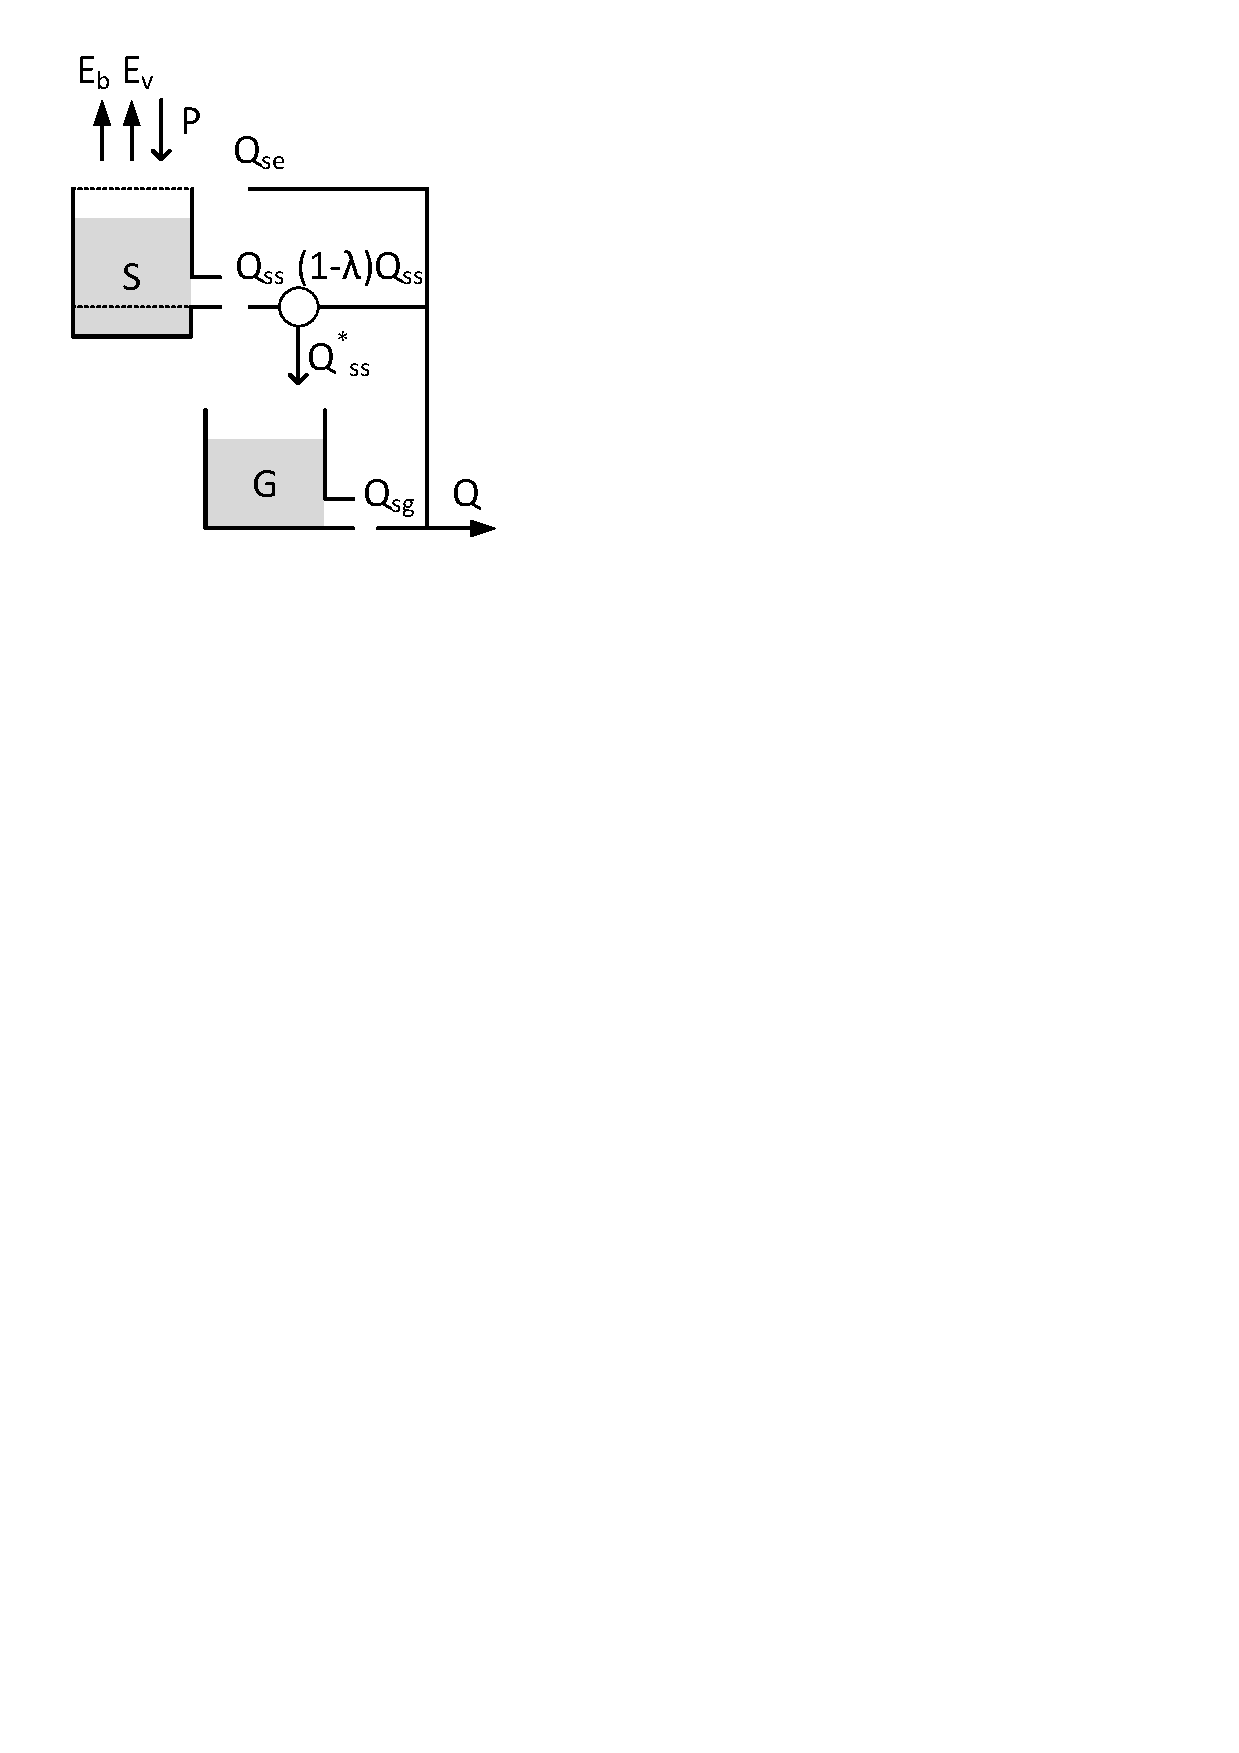
\includegraphics[trim=1cm 20cm 9cm 1cm,width=7cm,keepaspectratio]{./AppA_files/11_schematic.pdf}
\caption{Structure of the Collie River Basin 3 model} \label{fig:11_schematic}
\end{wrapfigure}

\begin{align}
	\frac{dS}{dt} &= P -E_b - E_v -Q_{se}-Q_{ss} \\
	Eb &= \frac{S}{S_{max}}(1-M)*Ep\\
	Ev &= 
		\begin{cases}
			M*E_p, & if~S>S_{fc}\\
			\frac{S}{S_{fc}}*M*E_p, &otherwise\\
		\end{cases}\\
	Q_{se} &= 
		\begin{cases}
			P, & if~S>S_{max}\\
			0, & otherwise \\
		\end{cases}\\
	Q_{ss} &= 
		\begin{cases}
			\big(a*(S-S{fc})\big)^b, & if~S>S_{fc}\\
			0, & otherwise 
		\end{cases}
\end{align}
}
\vspace{1.5cm}

Where  $S$ [mm] is the current storage in the soil moisture and $P$ the precipitation input $[mm/d]$. Actual evaporation is split between bare soil evaporation $E_b$ $[mm/d]$ and transpiration through vegetation $E_v$ $[mm/d]$, controlled through the forest fraction $M$. The evaporation estimates are based on the current storage $S$, the potential evapotranspiration $E_p$ $[mm/d]$ and the maximum soil moisture storage $S_{max}$ [mm], and field capacity $S_{fc}$ [mm] respectively. $Q_{se}$ $[mm/d]$ is saturation excess overland flow.  $Q_{ss}$ $[mm/d]$ is non-linear subsurface flow regulated by runoff coefficients $a$ $[d^{-1}]$ and $b$ [-].

\begin{align}
	\frac{dG}{dt} &= Q_{ss}^* - Q{sg} \\
	Q_{ss}^* &= \lambda*Q_{ss} \\
	Q_{sg} &= (a*G)^b
\end{align}

Where $G$ [mm] is groundwater storage. $Q_{ss}^*$ $mm/d]$ is the fraction $\lambda$ of $Q_{ss}$ directed to groundwater. $Q_{sg}$ $[mm/d]$ is non-linear groundwater flow that relies on the same parameters as subsurface flow uses. Total runoff:

\begin{equation}
	Q = Q_{se} + (1-\lambda)*Q_{ss} + Q_{sg}
\end{equation}


\subsection{Parameter overview}
% Table generated by Excel2LaTeX from sheet 'Sheet1'
\begin{table}[htbp]
  \centering
    \begin{tabular}{lll}
    \toprule
    Parameter & Unit  & Description \\
    \midrule
    $S_{max}$ & $mm$  & Maximum soil moisture storage \\
    $S_{fc}$ & $mm$  & Field capacity \\
    $a$   & $d^{-1}$ & Runoff coefficient \\
    $M$   & $-$   & Forest fraction \\
    $b$   & $-$   & Runoff nonlinearity \\
    $\lambda$ & $-$   & Fraction subsurface flow to groundwater \\
    \bottomrule
    \end{tabular}%
  \label{tab:addlabel}%
\end{table}%

\subsection{Alpine model v2 (model ID: 12)}
The Alpine model v2 (fig.~\ref{fig:12_schematic}) is part of a top-down modelling exercise and represents a daily water balance model \citep{Eder2003}. It has 2 stores and 6 parameters ($T_t$, $ddf$, $S_{max}$, $S_{fc}$, $t_{c,in}$, $t_{c,bf}$). The model aims to represent:

\begin{itemizecompact}
\item Snow accumulation and melt;
\item Saturation excess overland flow;
\item Linear subsurface runoff.
\end{itemizecompact}

\subsubsection{File names}
\begin{tabular}{@{}ll}
Model: &m\_12\_alpine2\_6p\_2s \\
Parameter ranges: &m\_12\_alpine2\_6p\_2s\_parameter\_ ranges \\
\end{tabular}

% Equations
\subsubsection{Model equations}

% Model layout figure
{ 																	% This ensures it doesn't warp text further down
\begin{wrapfigure}{l}{7cm}
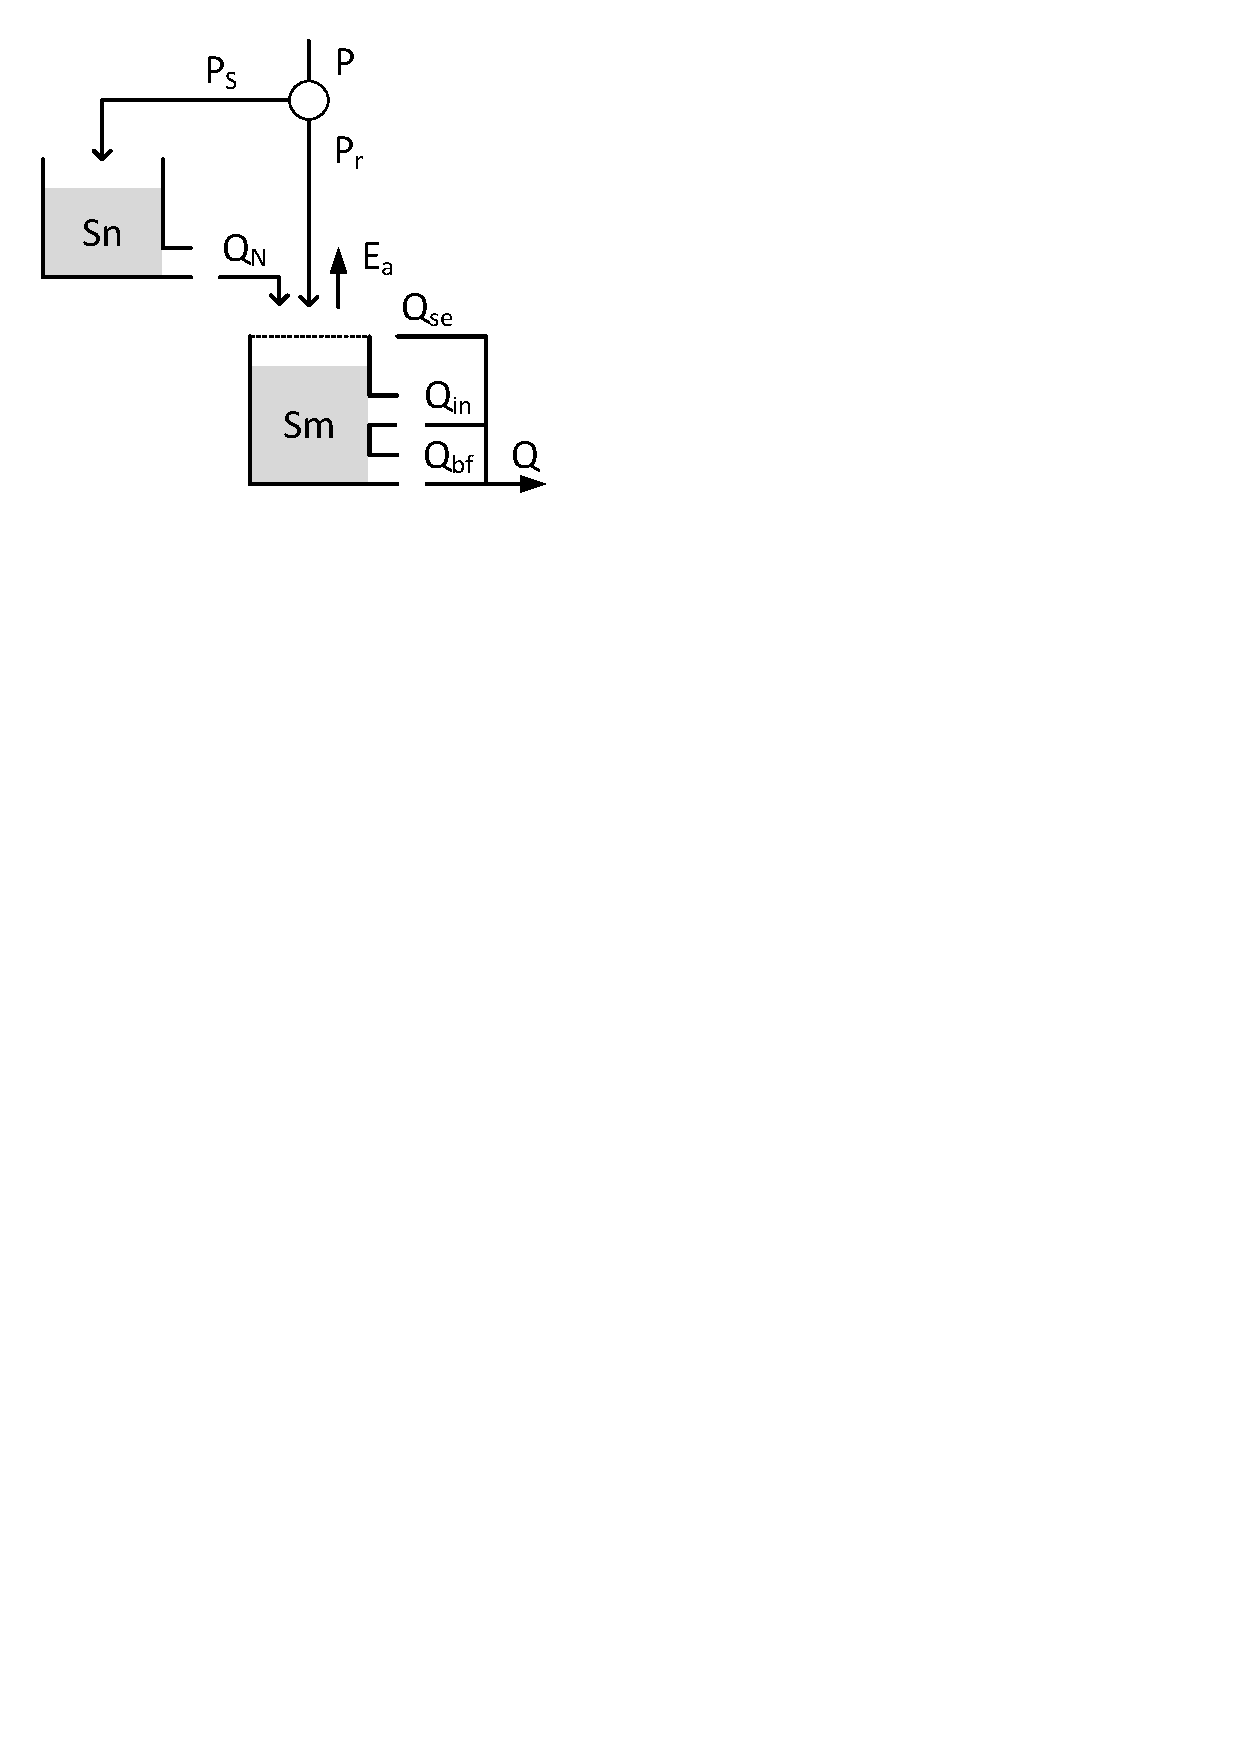
\includegraphics[trim=1cm 21.5cm 9cm 1cm,width=7cm,keepaspectratio]{./files/12_schematic.pdf}
\caption{Structure of the Alpine model v1} \label{fig:12_schematic}
\end{wrapfigure}

\begin{align}
	\frac{dSn}{dt} &= P_s-Q_N \\
	P_s &= \begin{cases}
		P, &\text{if } T \leq T_t \\
		0, & \text{otherwise} \\
	\end{cases} \\
	Q_N &= 
	\begin{cases}
		ddf*(T - T_t), & \text{if } T \geq T_t \\
		0, & \text{otherwise}
	\end{cases}
\end{align}

Where $S_N$ is the current snow storage [mm], $P_s$ the precipitation that falls as snow $[mm/d]$, $Q_N$ snow melt $[mm/d]$ based on a degree-day factor (ddf, [mm/\degree C/d]) and threshold temperature for snowfall and snowmelt ($T_t$, [\degree C]).

}

\begin{align}
	\frac{dS}{dt} &= P_r + Q_N - E_a  - Q_{se} - Q_{in} - Q_{bf}\\
	P_r &= \begin{cases}
		P, &\text{if } T > TT \\
		0, & \text{otherwise} \\
	\end{cases} \\
	E_a &= \begin{cases}
		E_p, &\text{if } S > 0 \\
		0, &\text{otherwise} \\
	\end{cases} \\
	Q_{se} &= \begin{cases}
		P_r + Q_N, &\text{if } S \geq S_{max}\\
		0, &\text{otherwise}\\
	\end{cases}\\
	Q_{in} &= \begin{cases}
		t_{c,in}*(S-S_{fc}), &\text{if } S > S_{fc} \\
		0, &\text{otherwise}\\
		\end{cases}\\
	Q_{bf} &= t_{c,bf}*S	
\end{align}

Where S [mm] is the current soil moisture storage, which is assumed to evaporate at the potential rate $E_p$ $[mm/d]$ when possible. When S exceeds the maximum storage $S_{max}$ [mm], water leaves the model as saturation excess runoff $Q_{se}$. If S exceeds field capacity $S_{fc}$ [mm], interflow $Q_{in}$ $[mm/d]$ is generated controlled by time parameter $t_{c,in}$ $[d^{-1}]$. $Q_{bf}$ represents baseflow controlled by time scale parameter $t_{c,bf}$ $[d^{-1}]$. Total runoff $Q_t$ $[mm/d]$ is:

\begin{equation}
	Q_t = Q_{se} + Q_{in} + Q_{bf}
\end{equation}

\subsubsection{Parameter overview}
% Table generated by Excel2LaTeX from sheet 'Sheet1'
\begin{table}[htbp]
  \centering
    \begin{tabular}{lll}
    \midrule
    Parameter & Unit  & Description \\
    \midrule
    $T_t$ & $^oC$ & Threshold temperature for snowfall and melt \\
    $ddf$ & $mm~^oC^{-1}~d^{-1}$ & Degree-day factor \\
    $S_{max}$ & $mm$  & Maximum soil moisture storage \\
    $S_{fc}$ & $mm$  & Field capacity \\
    $t_{c,in}$ & $d^{-1}$ & Runoff coefficient \\
    $t_{c,bf}$ & $d^{-1}$ & Runoff coefficient \\
    \bottomrule
    \end{tabular}%
  \label{tab:addlabel}%
\end{table}%

\subsection{Hillslope model (model ID: 13)}
The Hillslope model (fig.~\ref{fig:13_schematic}) is a conceptualization of the perceived dominant processes in a typical Western European hillslope \citep{Savenije2010}. It belongs to a 3-part topography driven modelling exercise, together with a wetland and plateau conceptualization. Each model is provided in isolation here, because they are well-suited for isolating specific model structure choices. It has 2 store and 7 parameters ($D_w$, $S_{h,max}$, $\beta_h$, $a$, $T_h$, $C$ and $K_h$). The model aims to represent:

\begin{itemizecompact}
\item Stylized interception by vegetation;
\item Evaporation;
\item Separation between rapid subsurface flow and groundwater recharge;
\item Capillary rise and linear relation runoff from groundwater.
\end{itemizecompact}

\subsubsection{File names}
\begin{tabular}{@{}ll}
Model: &m\_13\_hillslope\_7p\_2s \\
Parameter ranges: &m\_13\_hillslope\_7p\_2s\_parameter\_ ranges \\
\end{tabular}

% Equations
\subsubsection{Model equations}

% Model layout figure
{ 																	% This ensures it doesn't warp text further down
\begin{wrapfigure}{l}{7cm}
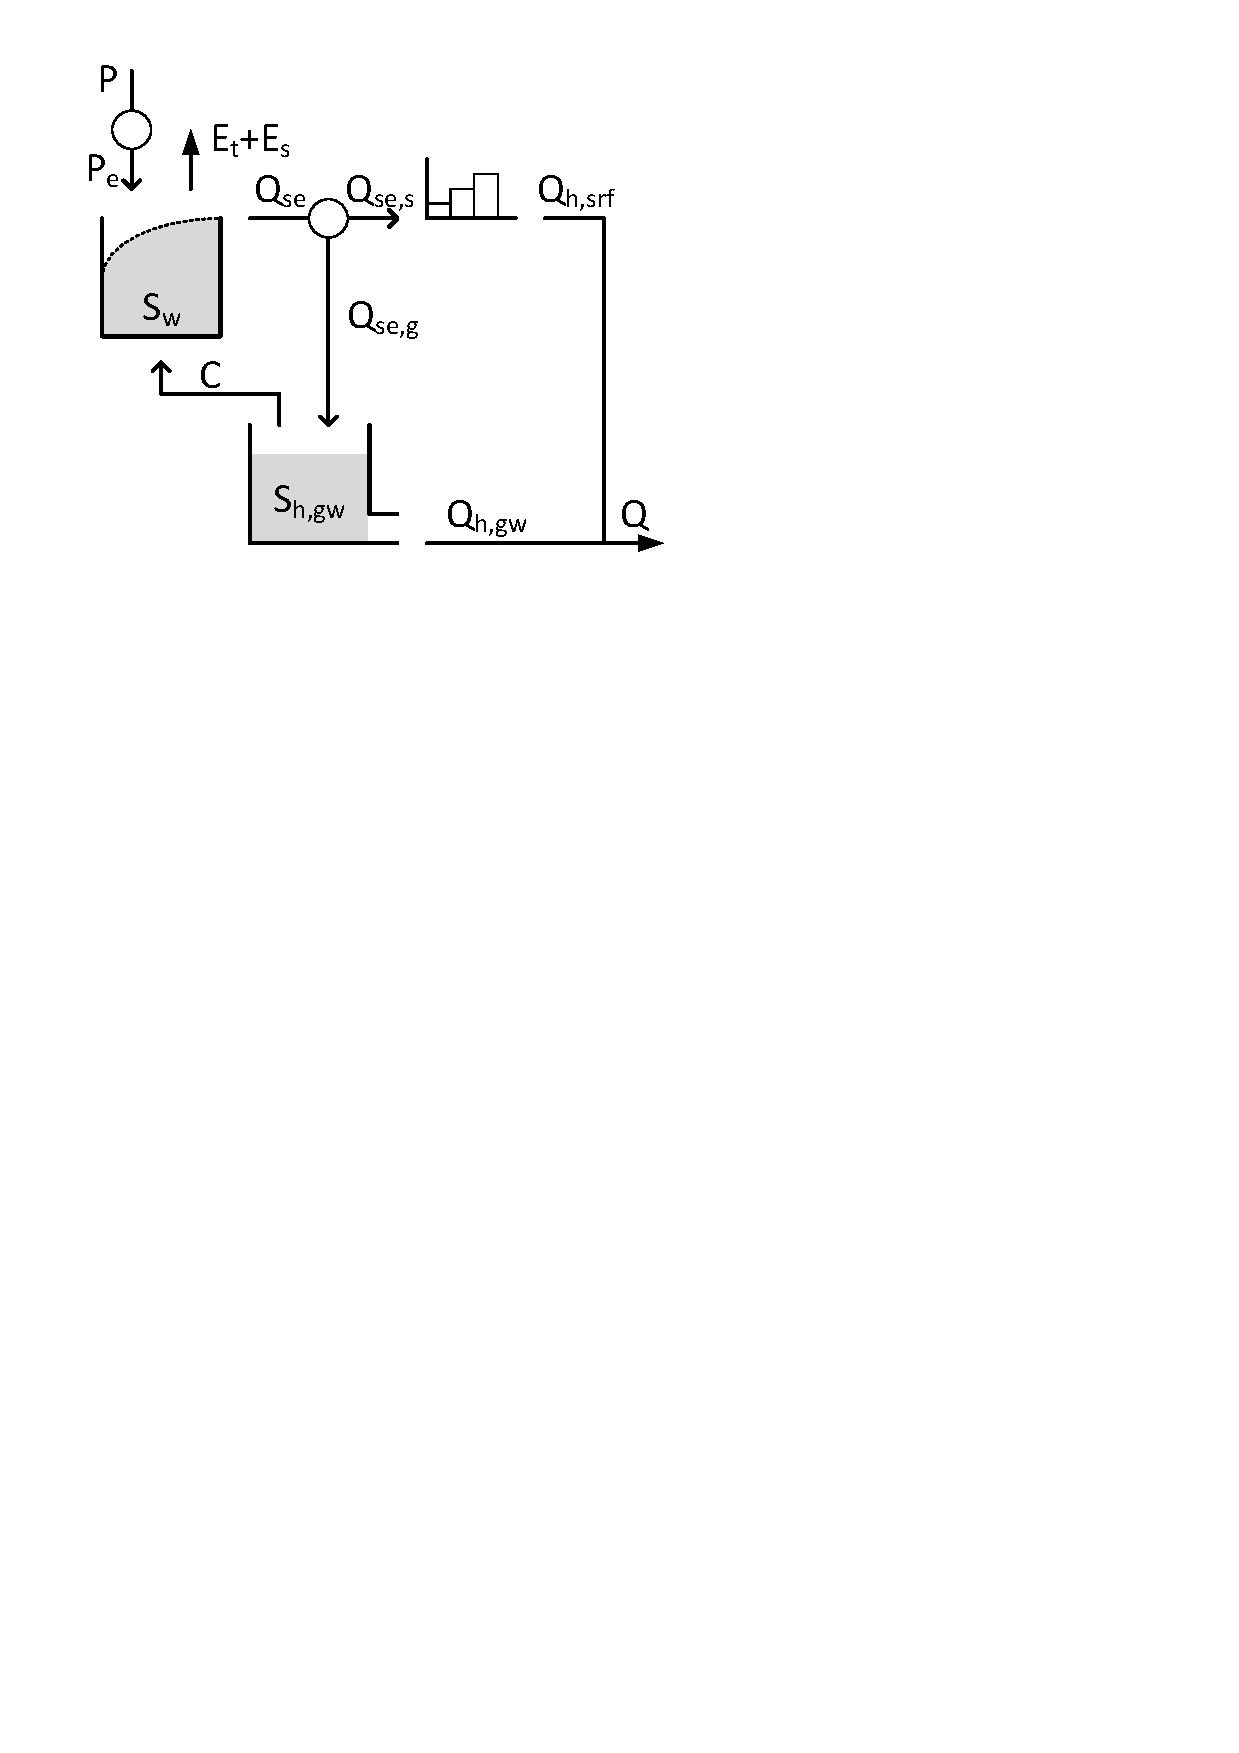
\includegraphics[trim=1cm 20.3cm 9cm 1cm,width=7cm,keepaspectratio]{./files/13_schematic.pdf}
\caption{Structure of the Hillslope model} \label{fig:13_schematic}
\end{wrapfigure}

\begin{align}
	\frac{dS_w}{dt} &= P_e+C-(E_t+E_s)-Q_{se} \\
	P_e &= max(P-D_h,0)\\
	C &= c.\\
	E_t+E_s &= 
	\begin{cases}
		E_p, & \text{if } S_w > 0 \\
		0, & \text{otherwise}\\
	\end{cases}\\
	Q_{se} &= \left(1-\left(1-\frac{S_h}{S_{h,max}}\right)^{\beta_h}\right)*P_e\\
\end{align}

Where $S_w$ is the current soil water storage [mm]. Incoming precipitation P [mm/d] is reduced by interception $D_h$ [mm/d], which is 

} % end of wrapfigure fix

assumed to evaporate before the next precipitation event. $C$ is capillary rise from groundwater [mm/d], given as a constant rate. Evaporation from soil moisture $E_t+E_s$ [mm/d] occurs at the potential rate $E_p$ whenever possible. Storage excess surface runoff $Q_{se}$ [mm/d] depends on the fraction of the catchment that is currently saturated, expressed through parameters $S_{h,max}$ [mm] and $\beta_h$ [-]. 

\begin{align}
	\frac{dS_{h,gw}}{dt} &= Q_{se,g}-C-Q_{h,gw} \\
	Q_{se,g} &= (1-a)*Q_{se}\\
	Q_{h,gw} &= K_h*S_{h,gw}
\end{align}

Where $S_{h,gw}$ is current groundwater storage [mm]. $Q_{se,g}$ is the groundwater fraction of storage excess flow $Q_{se}$ [mm/d], with $Q_{se,s}$ as its complementary part. $a$ is the parameter controlling this division [-]. Groundwater flow $Q_{h,gw}$ [mm/d] depends linearly on current storage $S_{h,gw}$ through parameter $K_h$ [$d^{-1}$]. Total flow $Q_t$ is the sum of $Q_{h,gw}$ and $Q_{h,srf}$, the latter of which is $Q_{se,s}$ lagged over $T_h$ days.

\subsubsection{Parameter overview}
% Table generated by Excel2LaTeX from sheet 'Sheet1'
\begin{table}[htbp]
  \centering
    \begin{tabular}{lll}
    \toprule
    Parameter & Unit  & Description \\
    \midrule
    $D_w$ & $mm~d^{-1}$ & Interception evaporation  \\
    $S_{h,max}$ & $mm$  & Maximum soil moisture storage \\
    $\beta_h$ & $-$   & Non-linearity parameter for contributing area \\
    $a$   & $-$   & Fraction saturation excess to groundwater \\
    $T_h$ & $d$   & Unit Hydrograph time base \\
    $C$   & $mm~d^{-1}$ & Capillary rise \\
    $K_h$ & $d^{-1}$ & Runoff coefficient \\
    \bottomrule
    \end{tabular}%
  \label{tab:addlabel}%
\end{table}%


\section{TOPMODEL (model ID: 14)}
The TOPMODEL (fig.~\ref{fig:14_schematic}) is originally a semi-distributed model that relies on topographic information \citep{BEVEN1979}. 
The model(ling concept) has undergone many revisions and significant differences can be seen between various publications. 
The version presented here is mostly based on \citet{Beven1995}, with several necessary simplifications. 
Following \citet{Clark2008a}, the model is simplified to a lumped model (removing the distributed routing component) and all parameters are calibrated. 
This means the distribution of topographic index values that characterizes TOPMODEL are estimated using a shifted 2-parameter gamma distribution instead of being based on DEM data \citep{Sivapalan1987,Clark2008a}. 
For simplicity of the evaporation calculations, the root zone store and unsaturated zone store are combined into a single threshold store with identical functionality to the original 2-store concept. 
The model has 2 stores and 7 parameters ($S_{UZ,max}$, $S_t$, $K_d$, $q_0$, $f$, $\chi$, $\phi$). 
The model aims to represent:

\begin{itemizecompact}
\item Variable saturated area with direct runoff from the saturated part;
\item Infiltration and saturation excess flow;
\item Leakage to, and non-linear baseflow from, a deficit store.
\end{itemizecompact}

\subsection{MARRMoT model name}
m\_14\_topmodel\_7p\_2s \\

% Equations
\subsection{Model equations}

% Model layout figure
{ 																	% This ensures it doesn't warp text further down
\begin{wrapfigure}{l}{4cm}
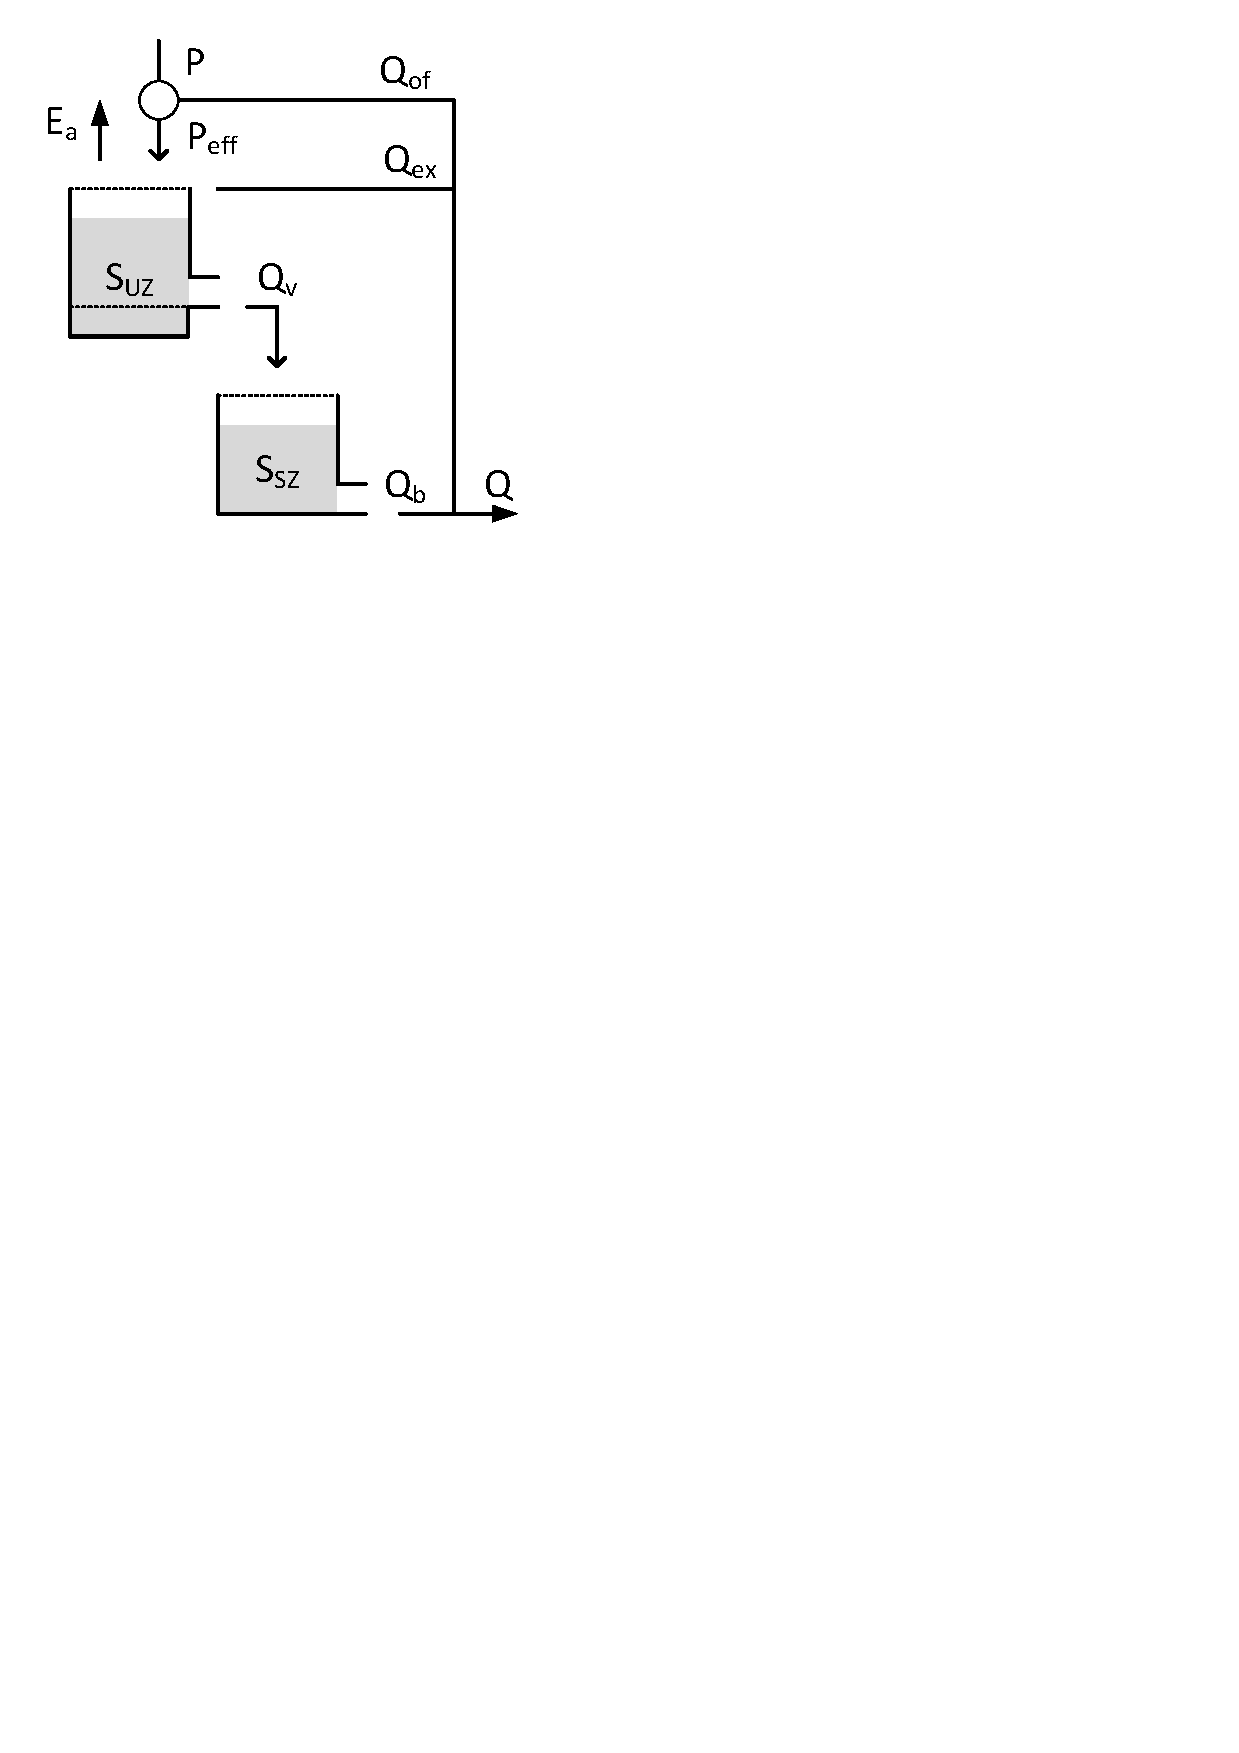
\includegraphics[trim=1cm 21cm 7cm 1cm,width=7cm,keepaspectratio]{./AppA_files/14_schematic.pdf}
\caption{Structure of the TOPMODEL} \label{fig:14_schematic}
\end{wrapfigure}

\begin{align}
	\frac{dS_{UZ}}{dt} &= P_{eff} - Q_{ex} - E_a - Q_v \\
	P_{eff} &= P - Q_{of} = P - A_C*P\\
	Q_{ex} &= \begin{cases}
		P_{eff}, & \text{if } S_{UZ} = S_{uz,max} \\
		0, & \text{otherwise}\\
	\end{cases}\\
	E_a &= 
	\begin{cases}
		E_p, & \text{if } S_{UZ} > S_t*S_{UZ,max} \\
		\frac{S_{UZ}}{S_t*S_{UZ,max}}*E_p, & \text{otherwise}\\
	\end{cases}\\	
	Q_v &=  
		\begin{cases}
		k_d\frac{S_{UZ} - S_t*S_{UZ,max}}{S_{UZ,max}(1-S_t)}, & \text{if } S_{UZ} > S_t*S_{UZ,max} \\
		0, & \text{otherwise}\\
	\end{cases}
\end{align}

} % end of wrapfigure fix
\vspace{0.5cm}

Where $S_{UZ}$ [mm] is the current storage in the combined unsaturated zone and root zone, with $S_t$ [-] (fraction of $S_{UZ,max}$) indicating the boundary between the two and being the threshold above which drainage to the saturated zone can occur. $P_{eff}$ $[mm/d]$ is the fraction of precipitation that does not fall on the saturated area $A_c$ [-], $E_a$ $[mm/d]$ is evaporation that occurs at the potential rate for the unsaturated zone and scaled linearly with storage in the root zone, $Q_{ex}$ $[mm/d]$ is overflow when the bucket reaches maximum capacity $S_{UZ,max}$ [mm], and $Q_v$ $[mm/d]$ is drainage to the saturated zone, depending on time parameter $k_d$ $[d^{-1}]$ and the relative storage in the unsaturated zone compared to the current deficit in the saturated zone.

\begin{align}
	\frac{dS_{SZ}}{dt} &= -Q_v + Q_b\\
	Q_b &= q_0*e^{-f*S_{SZ}}
\end{align}

Where $S_{SZ}$ [mm] is the current storage \emph{deficit} in the saturated zone store, which is increased by baseflow $Q_b$ $[mm/d]$ and decreased by drainage $Q_v$. $Q_b$ relies on saturated flow rate $q_0$ $[mm/d]$, parameter $f$ $[mm^{-1}]$ and current deficit $S_{SZ}$. Total flow:

\begin{align}
	Q &= Q_{of} + Q_{ex} + Q_b\\
	Q_{of} &= A_c*P
\end{align}

The saturated area $A_c$ is calculated as follows. First, the within-catchment distribution of topographic index values is estimated with a shifted 2-parameter gamma distribution \citep{Sivapalan1987,Clark2008a}:

\begin{align}
	f(\zeta) &= \begin{cases}
		\frac{1}{\chi\Gamma(\phi)}\left(\frac{\zeta-\mu}{\chi}\right)^{\phi-1}exp\left(-\frac{\zeta-\mu}{\chi}\right), & \text{if } \zeta > \mu \\
		0, & \text{otherwise}\\
	\end{cases}
\end{align}

Where $\Gamma$ is the gamma function and $\chi$, $\phi$ and $\mu$ are parameters of the gamma distribution. Following \citet{Clark2008a}, $\mu$ is fixed at $\mu=3$ and $\chi$ and $\phi$ are calibration parameters. $\zeta$ represents the topographic index $ln(a/tan\beta)$ with mean value $\lambda = \chi\phi+\mu$. Saturated area $A_c$ is computed as the fraction of the catchment that is above a deficit-dependent critical value $\zeta_{crit}$: 

\begin{align}
	A_c &= \int_{\zeta_{crit}}^{\infty}f(\zeta)d\zeta\\
	\zeta_{crit} &= f*S_{SZ} + \lambda
\end{align}

\newpage
\subsection{Parameter overview}
% Table generated by Excel2LaTeX from sheet 'Sheet1'
\begin{table}[htbp]
  \centering
    \begin{tabular}{lll}
    \toprule
    Parameter & Unit  & Description \\
    \midrule
    $S_{UZ,max}$ & $mm$  & Maximum soil moisture storage \\
    $S_t$ & $-$   & Threshold for drainage as fraction of $S_{UZ,max}$ \\
    $K_d$ & $d^{-1}$ & Runoff coefficient \\
    $q_0$ & $mm~d^{-1}$ & Saturated flow rate \\
    $f$   & $mm^{-1}$ & Shape parameter for connectivity profile \\
    $\chi$ & $-$   & Gamma distribution parameter \\
    $\phi$ & $-$   & Gamma distribution parameter \\
    \bottomrule
    \end{tabular}%
  \label{tab:addlabel}%
\end{table}%


\section{Plateau model (model ID: 15)}
The Plateau model (fig.~\ref{fig:15_schematic}) is a conceptualization of the perceived dominant processes in a typical Western European plateau \citep{Savenije2010}. It belongs to a 3-part topography driven modelling exercise, together with a wetland and hillslope conceptualization. Each model is provided in isolation here, because they are well-suited for isolating specific model structure choices. It has 2 stores and 8 parameters ($F_{max}$, $D_p$, $S_{u,max}$, $lp$, $p$, $T_p$, $C$ and $K_p$). The model aims to represent:

\begin{itemizecompact}
\item Stylized interception by vegetation;
\item Evaporation controlled by a wilting point and moisture constrained transpiration;
\item Separation between infiltration and infiltration excess flow;
\item Capillary rise and linear relation runoff from groundwater.
\end{itemizecompact}

\subsection{MARRMoT model name}
m\_15\_plateau\_8p\_2s \\

% Equations
\subsection{Model equations}

% Model layout figure
{ 																	% This ensures it doesn't warp text further down
\begin{wrapfigure}{l}{6cm}
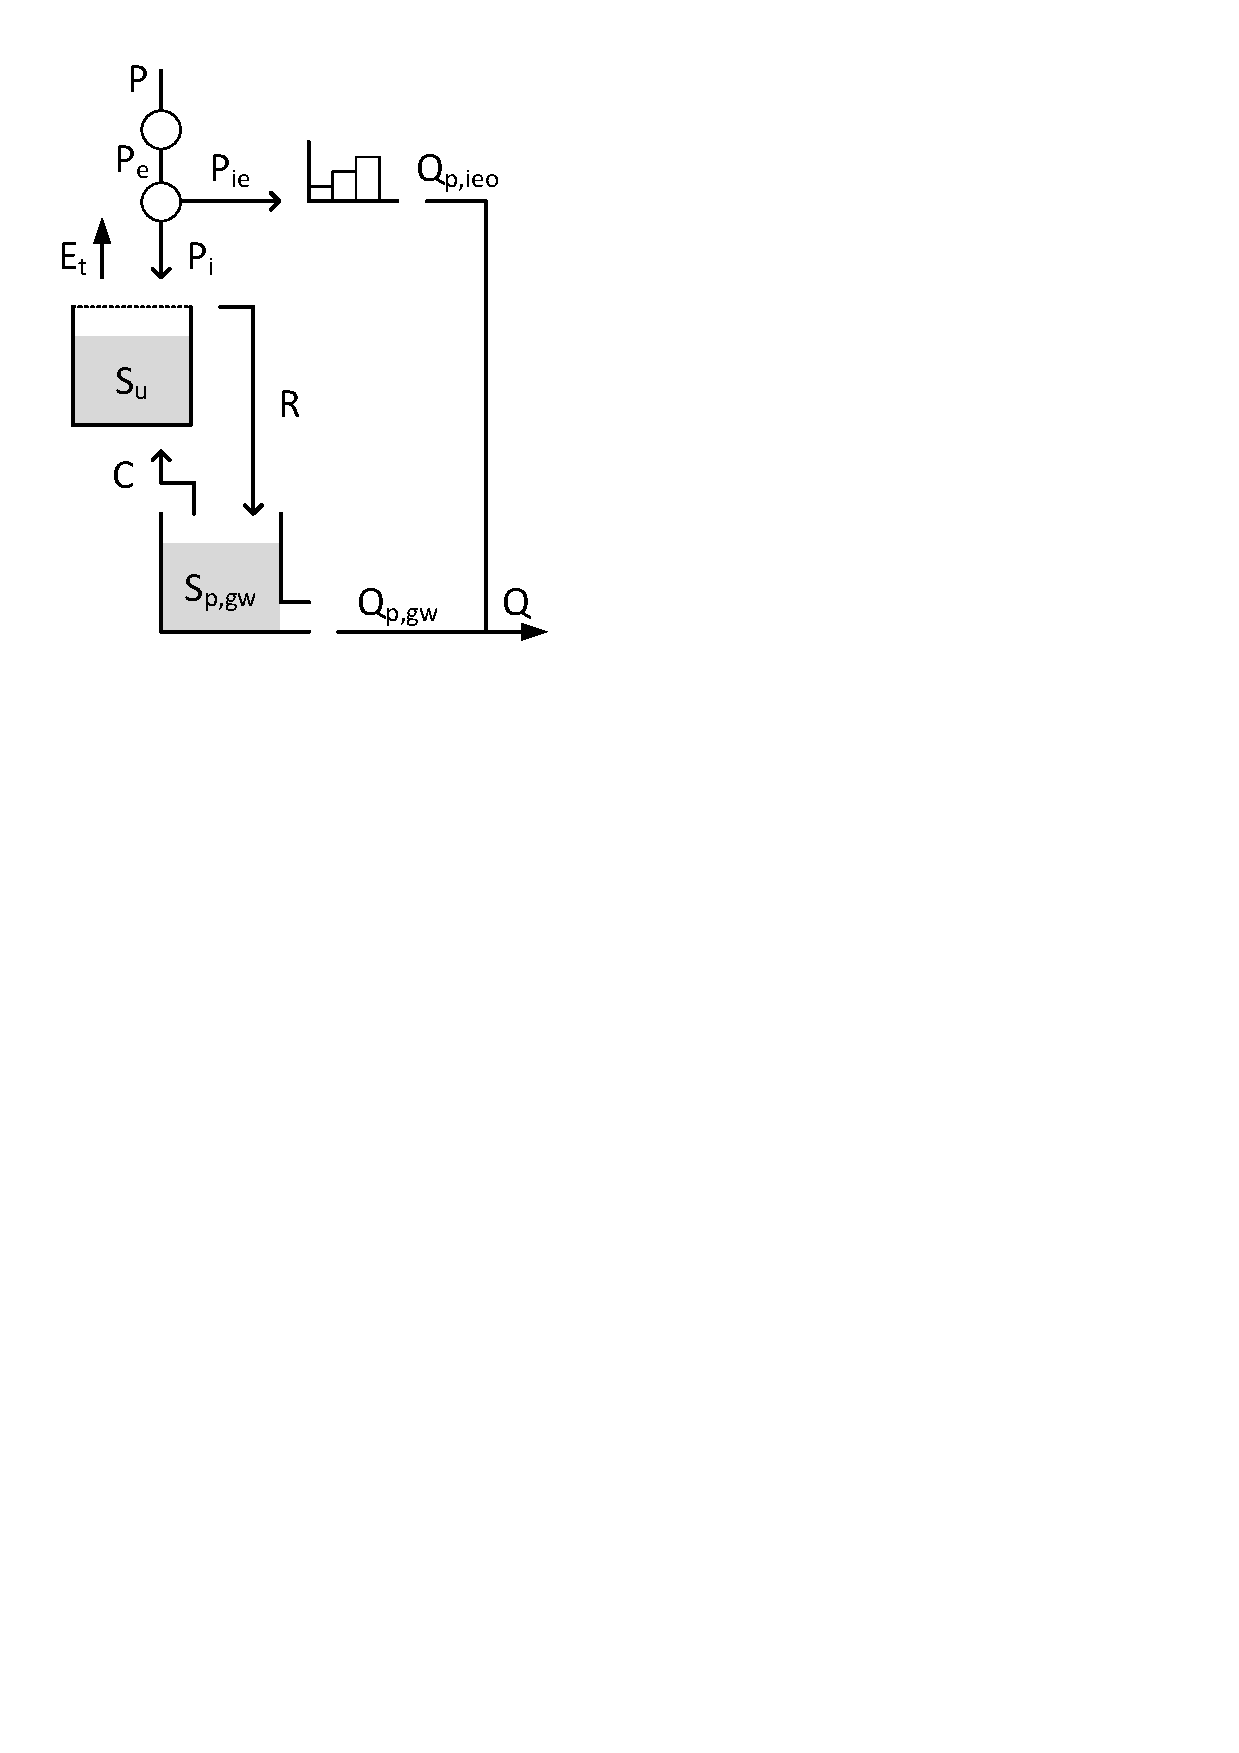
\includegraphics[trim=1cm 19cm 9cm 1cm,width=7cm,keepaspectratio]{./AppA_files/15_schematic.pdf}
\caption{Structure of the Plateau model} \label{fig:15_schematic}
\end{wrapfigure}

\begin{align}
	\frac{dS_u}{dt} &= P_i+C-E_t-R \\
	P_i &= min(P_e,F_{max})\\
		& = min\left(max(P-D_p,0),F_{max}\right)\\
	C &= c.\\
	E_t &= E_p*max\left(p\frac{S_u-S_{wp}}{S_{u,max}-S_{wp}},0\right)\\
	R &=	\begin{cases}
		P_i+C, & \text{if } S_u = S_{u,max} \\
		0, & \text{otherwise}\\
	\end{cases}
\end{align}

Where $S_u$ is the current soil water storage [mm]. Incoming precipitation P [mm/d] is reduced by interception $D_p$ [mm/d], which is assumed to evaporate before the next precipitation event. $P_e$ is further divided into infiltration $P_i$ [mm/d] based on the maximum infiltration rate $F_{max}$ [mm/d] and infiltration excess $P_{ie} = P_e-P_i$ [mm/d]. $C$ is capillary rise from ground water [mm/d], given as a constant rate.

 } % end of wrapfigure fix 

\noindent Evaporation from soil moisture $E_t$ [mm/d] occurs at the potential rate $E_p$ when $S_u$ is above the wilting point $S_{wp}$ [mm] (here defined as $S_{wp} = lp*S_{u,max}$) and is further constrained by coefficient $p$ [-], which is between 0 and 1. Storage excess $R$ [mm/d] flows into the groundwater. 

\begin{align}
	\frac{dS_{p,gw}}{dt} &=R-C-Q_{p,gw} \\
	Q_{p,gw} &= K_p*S_{p,gw}
\end{align}

Where $S_{p,gw}$ is current groundwater storage [mm]. Groundwater flow $Q_{p,gw}$ [mm/d] depends linearly on current storage $S_{p,gw}$ through parameter $K_p$ [$d^{-1}$]. Total flow $Q_t$ is the sum of $Q_{p,gw}$ and $Q_{p,ieo}$, the latter of which is $P_{ie}$ lagged over $T_p$ days.

\subsection{Parameter overview}
% Table generated by Excel2LaTeX from sheet 'Sheet1'
\begin{table}[htbp]
  \centering
    \begin{tabular}{lll}
    \toprule
    Parameter & Unit  & Description \\
    \midrule
    $F_{max}$ & $mm~d^{-1}$ & Maximum infiltration rate \\
    $D_p$ & $mm~d^{-1}$ & Interception evaporation  \\
    $S_{u,max}$ & $mm$  & Maximum soil moisture storage \\
    $lp$  & $-$   & Wilting point as fraction of $S_{u,max}$ \\
    $p$   & $-$   & Evaporation reduction factor \\
    $T_p$ & $d$   & Unit Hydrograph time base \\
    $C$   & $mm~d^{-1}$ & Capillary rise \\
    $K_p$ & $d^{-1}$ & Runoff coefficient \\
    \bottomrule
    \end{tabular}%
  \label{tab:addlabel}%
\end{table}%



\subsection{New Zealand model v2 (model ID: 16)}
The New Zealand model v2 (fig.~\ref{fig:16_schematic}) is part of a top-down modelling exercise (referred to as "Model A") that focusses on several catchments in New Zealand \citep{Atkinson2003}. It has 2 stores and 8 parameters ($I_{max}$, $S_{max}$, $S_{fc}$, $M$, $a$, $b$, $t_{c,bf}$ and $d$). The model aims to represent:

\begin{itemizecompact}
\item Interception by vegetation;
\item Separate vegetation and bare soil evaporation;
\item Saturation excess overland flow;
\item Subsurface runoff when soil moisture exceeds field capacity;
\item Baseflow;
\item Flow routing.
\end{itemizecompact}

\subsubsection{File names}
\begin{tabular}{@{}ll}
Model: &m\_16\_newzealand2\_8p\_2s \\
Parameter ranges: &m\_16\_newzealand2\_8p\_2s\_parameter\_ ranges \\
\end{tabular}

% Equations
\subsubsection{Model equations}

% Model layout figure
{ 																	% This ensures it doesn't warp text further down
\begin{wrapfigure}{l}{6.5cm}
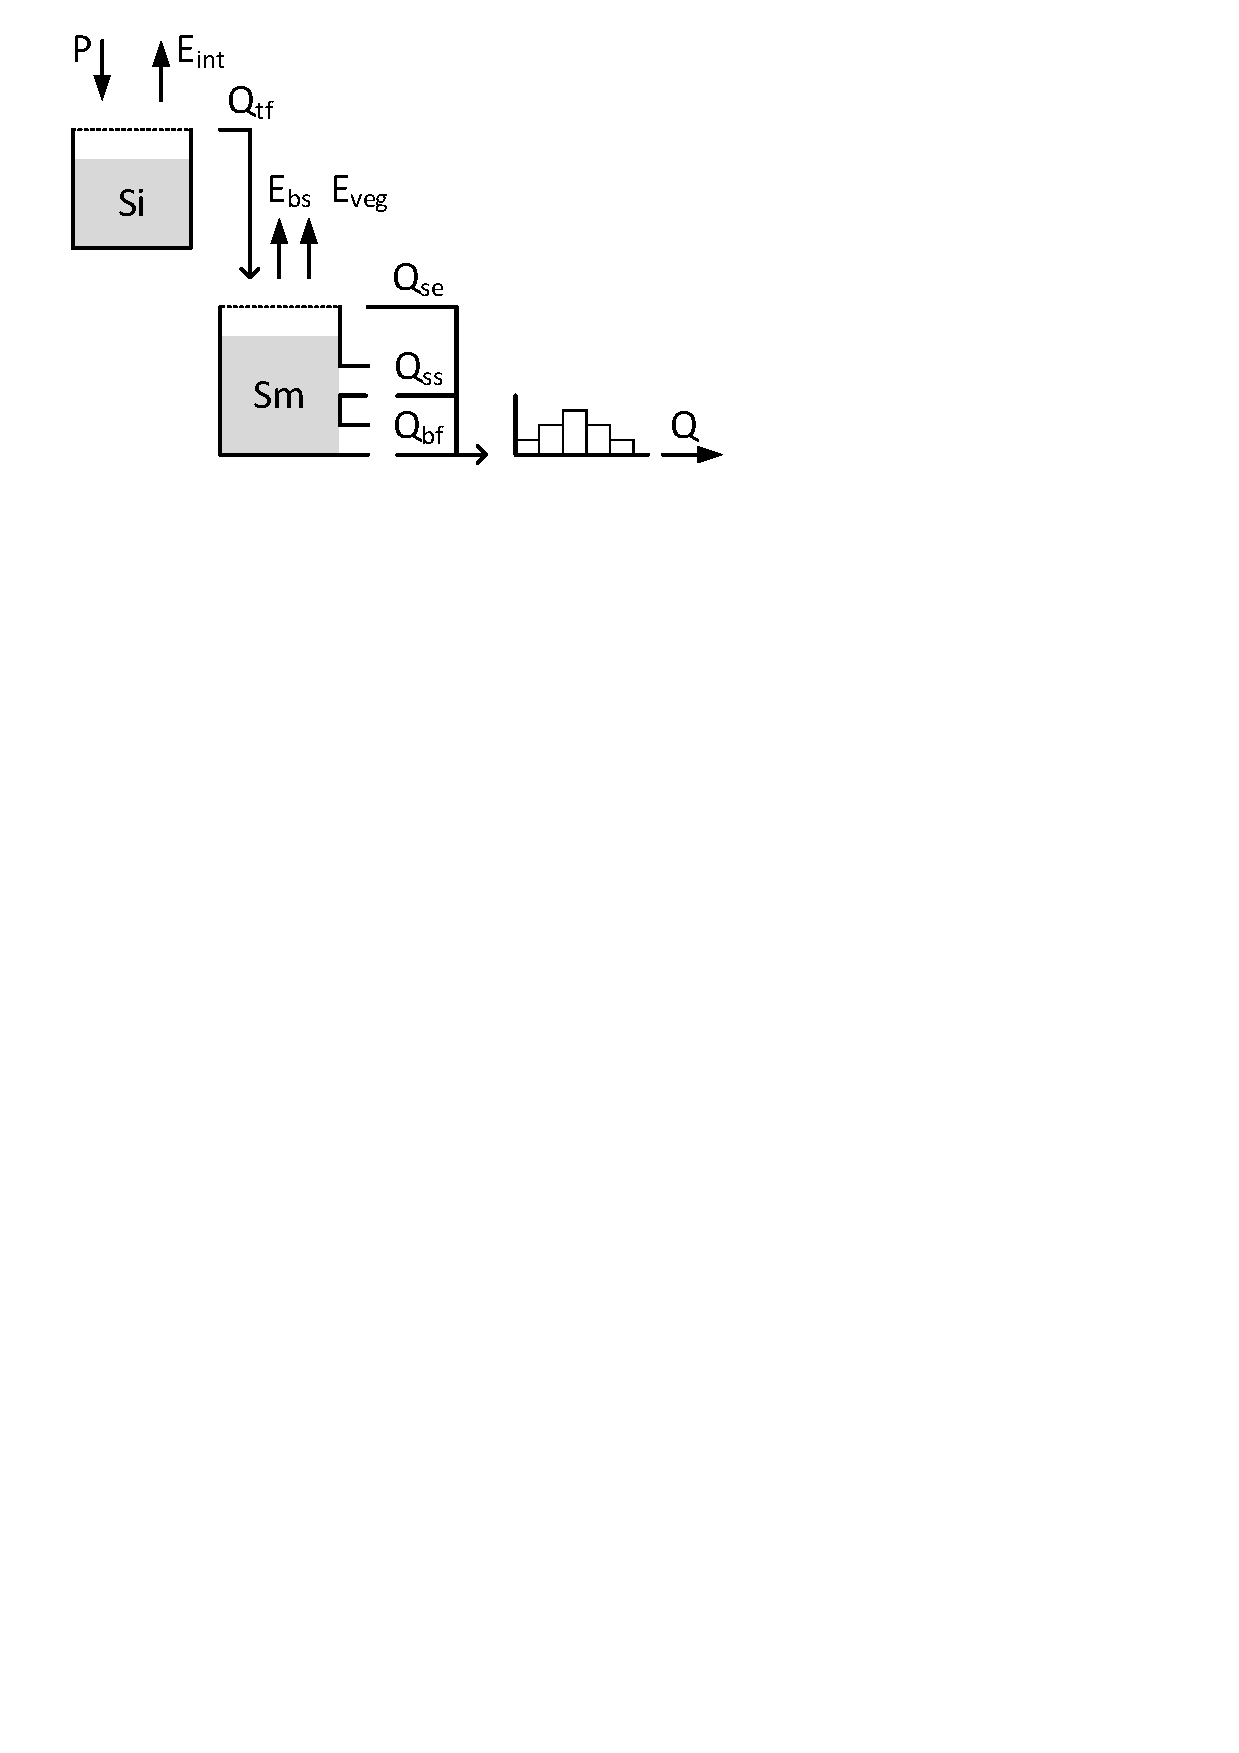
\includegraphics[trim=1cm 22cm 7cm 1cm,width=7cm,keepaspectratio]{./files/16_schematic.pdf}
\caption{Structure of the New Zealand model v1} \label{fig:16_schematic}
\end{wrapfigure}

\begin{align}
	\frac{dS_i}{dt} &= P - E_{int} - Q_{tf}\\
	E_{int} &= Ep \\
	Q_{tf} &= \begin{cases}
		P, &\text{if } S_i \geq I_{max}\\
		0, &\text{otherwise}\\
	\end{cases}
\end{align}

Where  $S_i$ [mm] is the current interception storage which gets replenished through daily precipitation $P$ $[mm/d]$. Intercepted water is assumed to evaporate ($E_{int}$ $[mm/d]$) at the potential rate $E_p$ $[mm/d]$ when possible. $Q_{tf}$ $[mm/d]$ represents throughfall towards soil moisture when the interception store is at maximum capacity $I_{max}$ [mm].

} % end of wrapfigure fix

\begin{align}
	\frac{dS_m}{dt} &= Q_{tf} - E_{veg} - E_{bs}  - Q_{se} - Q_{ss} - Q_{bf}\\
	E_{veg} &= \begin{cases}
		M*E_p, &\text{if } S > S_{fc} \\
		\frac{S_m}{S_{fc}}*M*E_p, &\text{otherwise} \\
	\end{cases} \\
	E_{bs} &= \frac{S}{S_{max}}(1-M)*E_p \\
	Q_{se} &= \begin{cases}
		P, &\text{if } S \geq S_{max}\\
		0, &\text{otherwise}\\
	\end{cases}\\
	Q_{ss} &= \begin{cases}
		\left(a*(S-S_{fc})\right)^b, &\text{if } S \geq S_{fc} \\
		0, &\text{otherwise}\\
		\end{cases}\\
	Q_{bf} &= t_{c,bf}*S	
\end{align}

Where $S_m$ [mm] is the current soil moisture storage which gets replenished through daily precipitation $P$ $[mm/d]$. Evaporation through vegetation $E_{veg}$ $[mm/d]$ depends on the forest fraction $M$ [-] and field capacity $S_{fc}$ [-]. $E_{bs}$ $[mm/d]$ represents bare soil evaporation. When S exceeds the maximum storage $S_{max}$ [mm], water leaves the model as saturation excess runoff $Q_{se}$. If S exceeds field capacity $S_{fc}$ [mm], subsurface runoff $Q_{ss}$ $[mm/d]$ is generated controlled by time parameter $a$ $[d^{-1}]$ and nonlinearity parameter $b$ [-]. $Q_{bf}$ represents baseflow controlled by time scale parameter $t_{c,bf}$ $[d^{-1}]$. Total runoff $Q_t$ $[mm/d]$ is:

\begin{equation}
	Q_t = Q_{se} + Q_{ss} + Q_{bf}
\end{equation}

Total flow is delayed by a triangular routing scheme controlled by time parameter $d$ [d].

\subsubsection{Parameter overview}
% Table generated by Excel2LaTeX from sheet 'Sheet1'
\begin{table}[htbp]
  \centering
    \begin{tabular}{lll}
    \toprule
    Parameter & Unit  & Description \\
    \midrule
    $I_{max}$ & $mm$  & Maximum interception capacity \\
    $S_{max}$ & $mm$  & Maximum soil moisture storage \\
    $S_{fc}$ & $mm$  & Field capacity \\
    $M$   & $-$   & Forest fraction \\
    $a$   & $d^{-1}$ & Runoff coefficient \\
    $b$   & $-$   & Runoff nonlinearity \\
    $t_{c,bf}$ & $d^{-1}$ & Runoff coefficient \\
    $d$   & $d$   & Unit Hydrograph time base \\
    \bottomrule
    \end{tabular}%
  \label{tab:addlabel}%
\end{table}%


\subsection{Penman model (model ID: 17)}
The Penman model (fig.~\ref{fig:17_schematic}) is based on the drying curve concept described in \citet{PENMAN1950} \citep{Wagener2002}. It has 3 stores and 4 parameters ($S_{max}$, $\phi$, $\gamma$, $k_1$). The model aims to represent:

\begin{itemizecompact}
\item Moisture accumulation and evaporation from the root zone;
\item Bypass of excess moisture to the stream;
\item Deficit-based groundwater accounting;
\item Linear flow routing.
\end{itemizecompact}

\subsubsection{File names}
\begin{tabular}{@{}ll}
Model: &m\_17\_penman\_4p\_3s \\
Parameter ranges: &m\_17\_penman\_4p\_3s\_parameter\_ ranges \\
\end{tabular}

% Equations
\subsubsection{Model equations}

% Model layout figure
{ 																	% This ensures it doesn't warp text further down
\begin{wrapfigure}{l}{4.5cm}
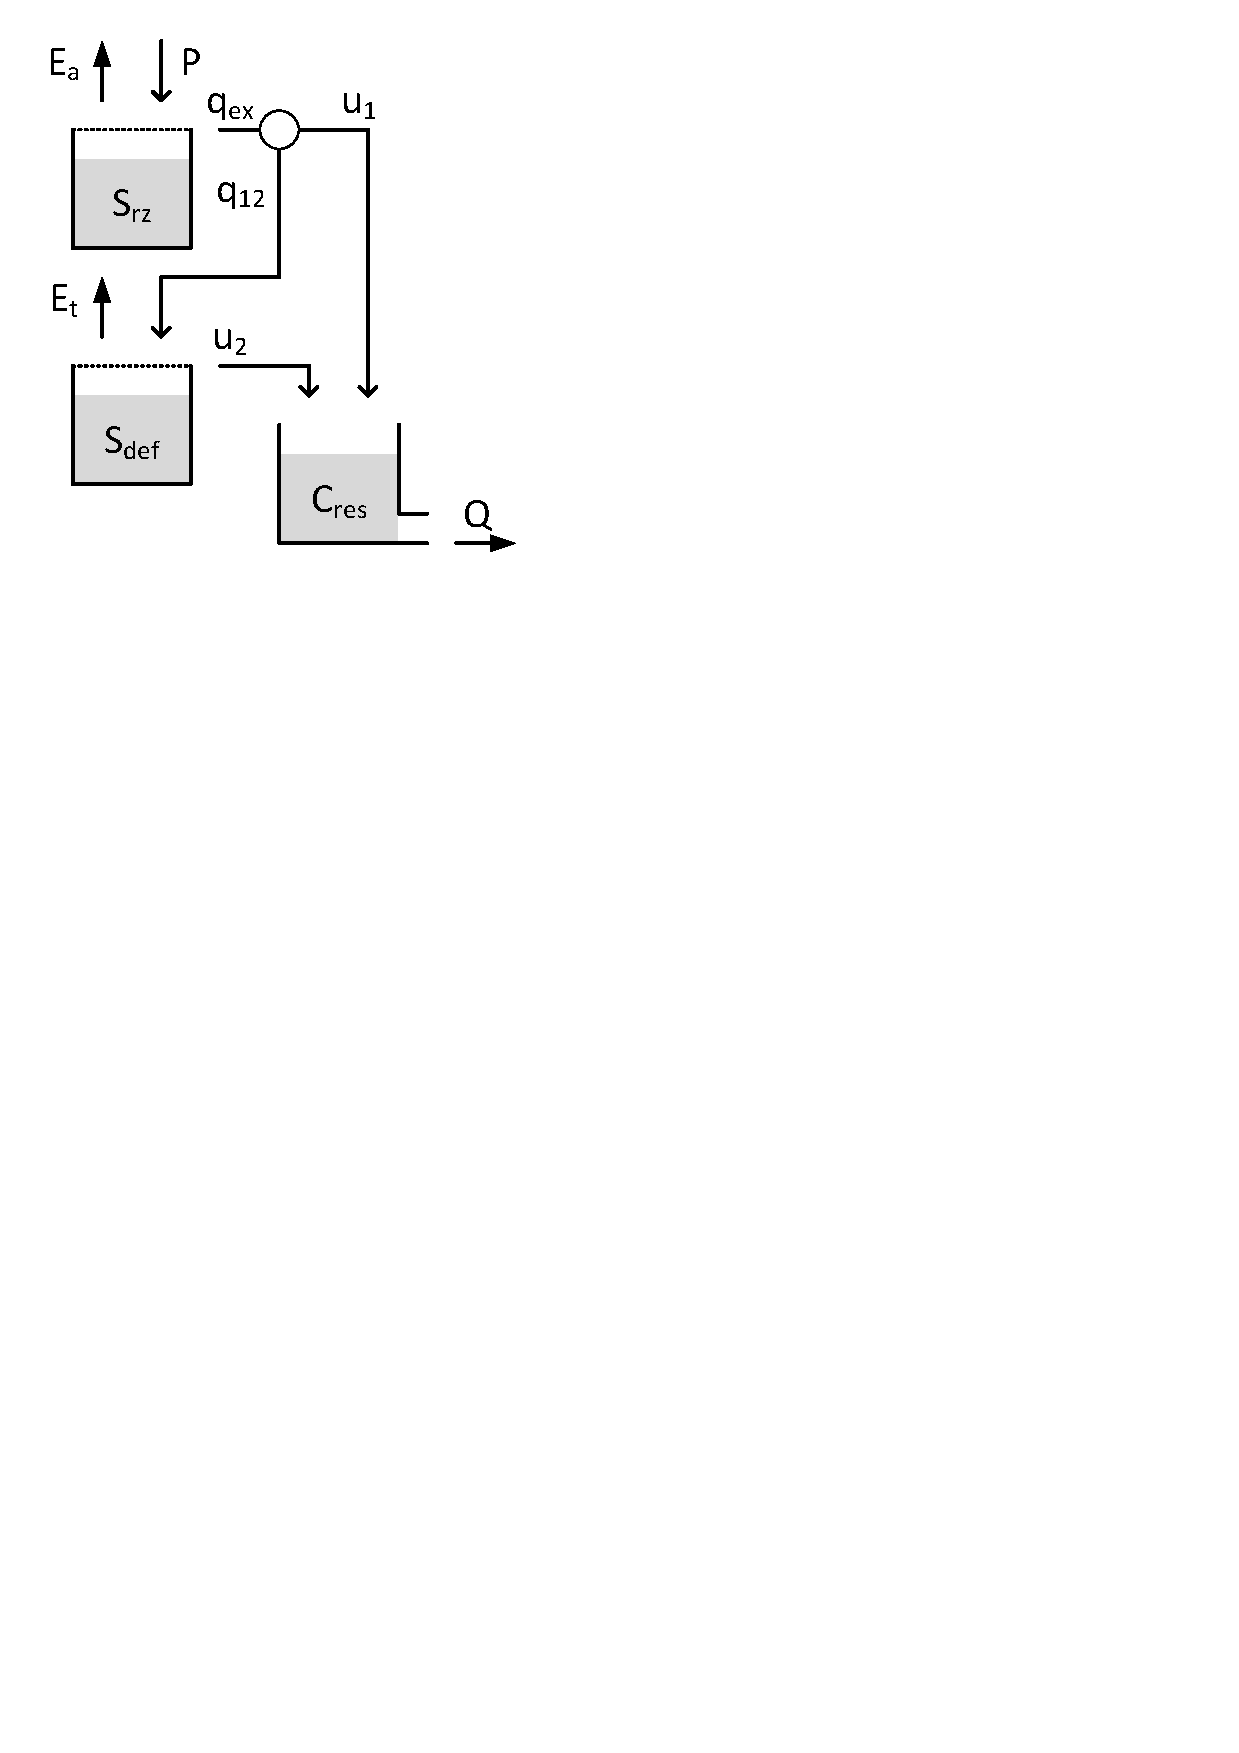
\includegraphics[trim=1cm 20cm 7cm 1cm,width=7cm,keepaspectratio]{./files/17_schematic.pdf}
\caption{Structure of the Penman model} \label{fig:17_schematic}
\end{wrapfigure}

\begin{align}
	\frac{dS_{rz}}{dt} &= P-E_a-q_{ex} \\
	E_a &= \begin{cases}
		E_p, &\text{if } S_{rz} > 0 \\
		0, & \text{otherwise} \\
	\end{cases} \\
	q_{ex} &= 
	\begin{cases}
		P, & \text{if } S_{rz} = S_{max} \\
		0, & \text{otherwise}
	\end{cases}
\end{align}

Where $S_{rz}$ [mm] is the current storage in the root zone, refilled by precipitation $P$ $[mm/d]$ and drained by evaporation $E_a$  $[mm/d]$ and moisture excess $q_{ex}$  $[mm/d]$. $E_a$ occurs at the potential rate $E_p$  $[mm/d]$ whenever possible. $q_{ex}$ occurs only when the store is at maximum capacity $S_{max}$ [mm].

} % end of wrapfigure fix

\begin{align}
	\frac{dS_{def}}{dt} &= E_t+u_2-q_{12}\\
	E_t &= \begin{cases}
		\gamma*E_p, &\text{if } S_{rz} = 0 \\
		0, &\text{otherwise} \\
	\end{cases} \\
	u_2 &= \begin{cases}
		q_{12}, &\text{if } S_{def} = 0\\
		0, &\text{otherwise}\\
	\end{cases}	\\
	q_{12} &= (1-\phi)*q_{ex}
\end{align}

Where $S_{def}$ [mm] is the current moisture \emph{deficit}, which is increased by evaporation $E_t$ $[mm/d]$ and reduced by inflow $q_{12}$ $[mm/d]$. 
$E_t$ occurs only when the upper store $S_{rz}$ is empty and at a fraction $\gamma$ [-] of $E_p$. 
Inflow $q_{12}$ is the fraction $(1-\phi)$ [-] of $q_{ex}$ that does not bypass the lower soil layer. 
Saturation excess $u_2$ $[mm/d]$ occurs only when there is zero deficit.

\begin{align}
	\frac{dC_{res}}{dt} &= u_1+u_2-Q\\
	u_1 &= \phi*q_{ex}\\
	Q &= k_1*C_{res}
\end{align}
  
Where $C_{res}$ [mm] is the current storage in the routing reservoir, increased by $u_1$ and $u_2$, and drained by runoff $Q$  $[mm/d]$. $u_1$ is the fraction $\phi$ of $q_{ex}$. $Q$ has a linear relationship with storage through time scale parameter $k_1$ $[d^{-1}]$.

\subsubsection{Parameter overview}

% Table generated by Excel2LaTeX from sheet 'Sheet1'
\begin{table}[htbp]
  \centering
    \begin{tabular}{lll}
    \toprule
    Parameter & Unit  & Description \\
    \midrule
    $S_{max}$ & $mm$  & Maximum soil moisture storage \\
    $\phi$ & $-$   & Fraction of saturation excess that is direct runoff \\
    $\gamma$ & $-$   & Evaporation reduction factor \\
    $k_1$ & $d^{-1}$ & Runoff coefficient \\
    \bottomrule
    \end{tabular}%
  \label{tab:addlabel}%
\end{table}%



\subsection{SIMHYD (model ID: 18)}
The SIMHYD model (fig.~\ref{fig:18_schematic}) is a simplified version of MODHYDROLOG, originally developed for use in Australia \citep{Chiew2002}. It has 3 stores and 7 parameters (INSC, COEFF, SQ, SMSC, SUB, CRAK and K). The model aims to represent:

\begin{itemizecompact}
\item Interception by vegetation;
\item Infiltration and infiltration excess flow;
\item Preferential groundwater recharge, interflow and saturation excess flow;
\item Groundwater recharge resulting from filling up of soil moisture storage capacity;
\item Slow flow from groundwater.
\end{itemizecompact}

\subsubsection{File names}
\begin{tabular}{@{}ll}
Model: &m\_18\_simhyd\_7p\_3s \\
Parameter ranges: &m\_18\_simhyd\_7p\_3s\_parameter\_ ranges \\
\end{tabular}

% Equations
\subsubsection{Model equations}

% Model layout figure
{ 																	% This ensures it doesn't warp text further down
\begin{wrapfigure}{l}{5cm}
\scalebox{0.7}{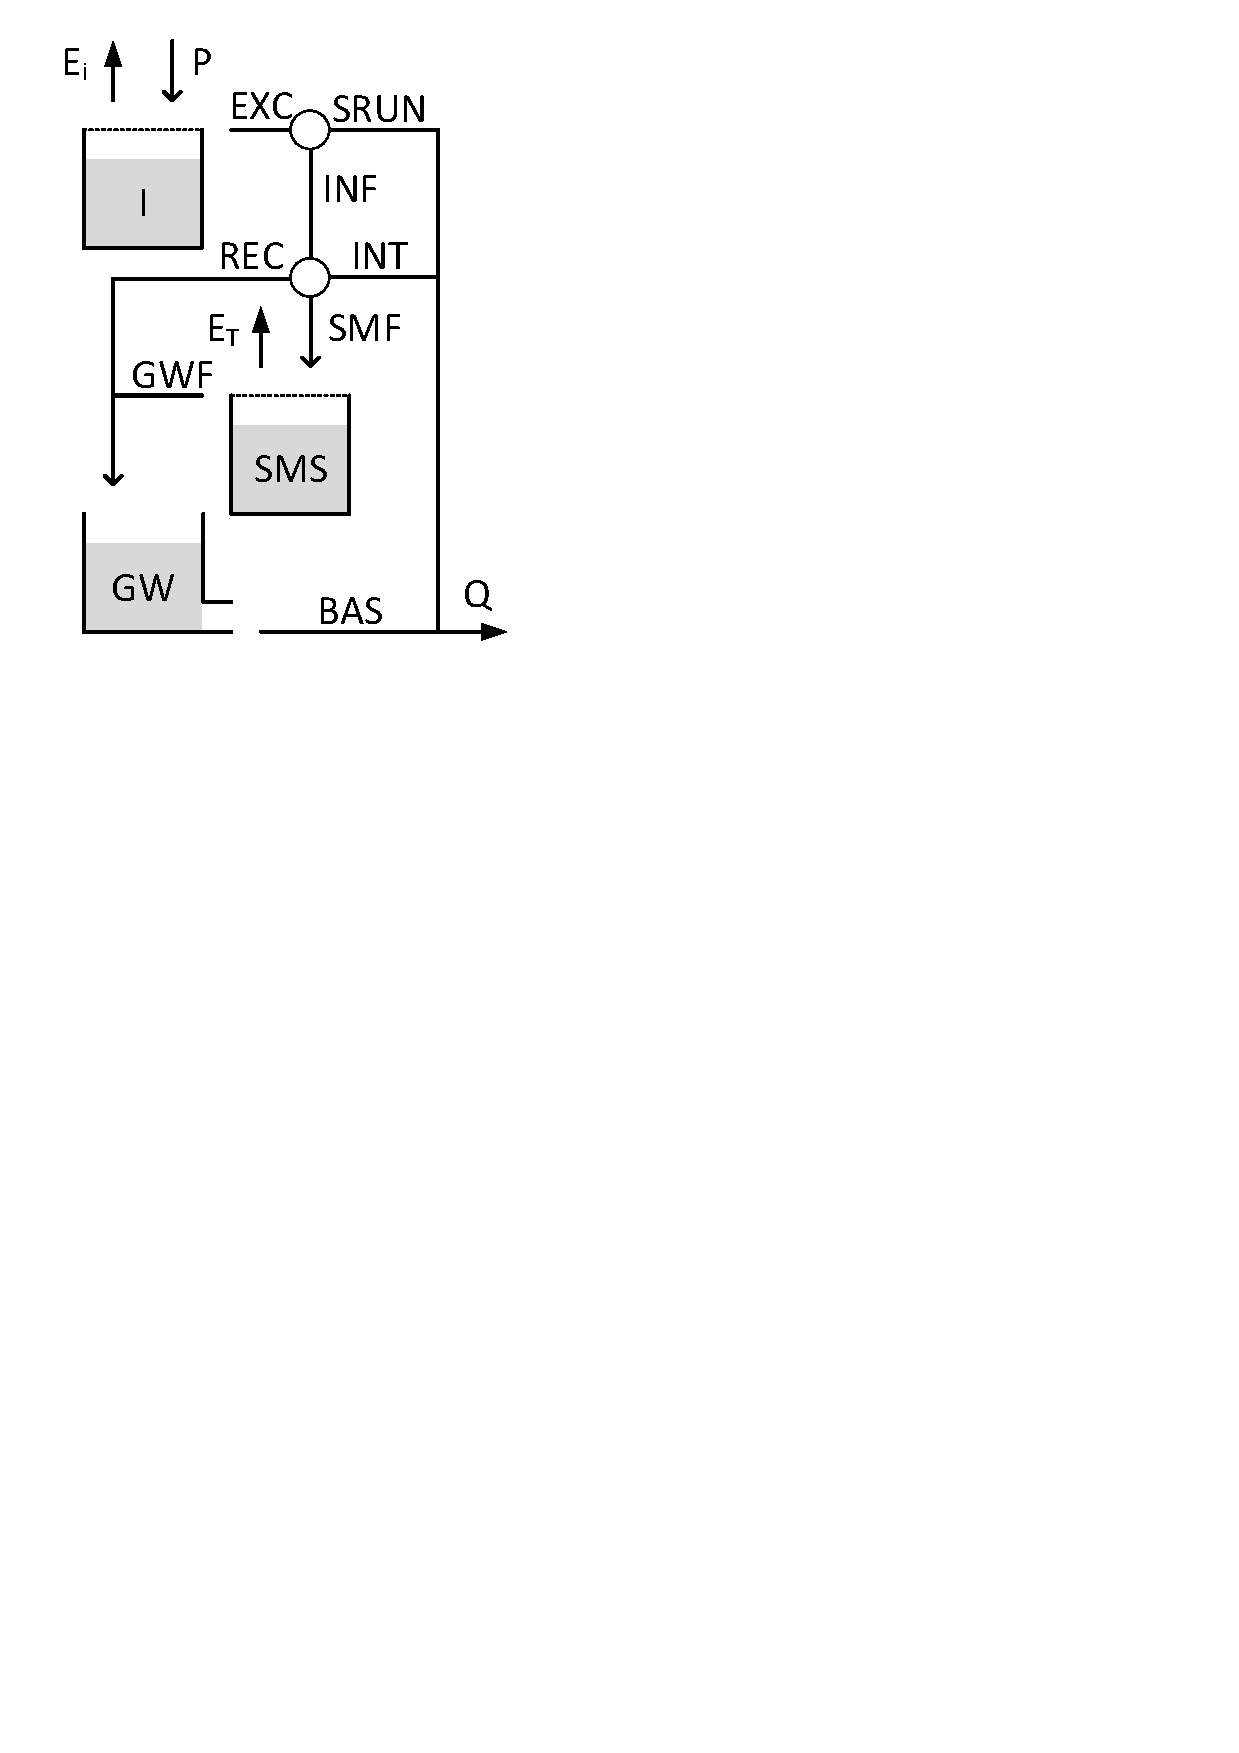
\includegraphics[trim=1cm 18cm 11.5cm 1cm,width=7cm,keepaspectratio]{./files/18_schematic.pdf}}
\caption{Structure of the SIMHYD model} \label{fig:18_schematic}
\end{wrapfigure}

\begin{align}
	\frac{dI}{dt} &= P-E_i-EXC \\
	E_i &= \begin{cases}
		E_p, &\text{if } I > 0 \\
		0, & \text{otherwise} \\
	\end{cases} \\
	EXC &= 
	\begin{cases}
		P, & \text{if } I = INSC \\
		0, & \text{otherwise}
	\end{cases}
\end{align}

Where I is the current interception storage [mm], $P$ precipitation [mm/d], $E_i$ the evaporation from the interception store [mm/d] and $EXC$ the excess rainfall [mm/d]). Evaporation is assumed to occur at the potential rate when possible. When I exceeds the maximum interception capacity $INSC$ [mm], water is routed to the rest of the model as excess precipitation $EXC$. 

} % end of wrapfigure
\vspace{1cm}
\begin{align}
	\frac{dSMS}{dt} &= SMF-E_T-GWF\\
	SMF &= INF-INT-REC\\
		&INF = min\left(COEFF * exp\left(\frac{-SQ*SMS}{SMSC}\right),EXC\right)\\
		&INT = SUB*\frac{SMS}{SMSC} * INF \\
		&REC = CRAK*\frac{SMS}{SMSC}*(INF-INT)\\
	E_T &=min\left(10*\frac{SMS}{SMSC},PET\right)\\
	GWF &= \begin{cases}
		SMF, &\text{if } SMS = SMSC\\
		0, &\text{otherwise}
	\end{cases}
\end{align}

Where SMS is the current storage in the soil moisture store [mm]. INF is total infiltration [mm/d] from excess precipitation, based on maximum infiltration loss parameter COEFF [mm/d], the infiltration loss exponent SQ [-] and the ratio between current soil moisture storage SMS and the maximum soil moisture capacity SMSC [mm]. INT represents interflow and saturation excess flow [mm/d], using a constant of proportionality SUB [-]. REC is preferential recharge of groundwater [mm/d] based on another constant of proportionality CRAK [-]. SMF is flow into soil moisture storage [mm/d]. $E_T$ evaporation from the soil moisture that occurs at the potential rate when possible [mm/d], and GWF the flow to the groundwater store [mm/d]:

\begin{align}
	\frac{dGW}{dt} &= REC+GWF - BAS\\
	BAS &= K * GW 
\end{align}

Where GW is the current storage [mm] in the groundwater reservoir. Outflow $BAS$ [mm/d] from the reservoir has a linear relation with storage through the linear recession parameter $K$ [$d^{-1}$]. Total outflow $Q_t$ [mm/d] is the sum of three parts:

\begin{align}
	Q_t &= SRUN+INT+BAS\\
	SRUN &= EXC-INF
\end{align}

\newpage
\subsubsection{Parameter overview}
% Table generated by Excel2LaTeX from sheet 'Sheet1'
\begin{table}[htbp]
  \centering
    \begin{tabular}{lll}
    \toprule
    Parameter & Unit  & Description \\
    \midrule
    INSC  & $mm$  & Maximum interception capacity \\
    COEFF & $mm~d^{-1}$ & Maximum infiltration loss \\
    SQ    & $-$   & Infiltration loss exponent \\
    SMSC  & $mm$  & Maximum soil moisture storage \\
    SUB   & $-$   & Proportionality constant \\
    CRAK  & $-$   & Proportionality constant \\
    K     & $d^{-1}$ & Runoff coefficient \\
    \bottomrule
    \end{tabular}%
  \label{tab:addlabel}%
\end{table}%




\subsection{Australia model (model ID: 19)}
The Australia model (fig.~\ref{fig:19_schematic}) is part of a top-down modelling exercise (originally referred to as model S4) designed to use auxiliary data \citep{Farmer2003}. 
Some adjustments were made to the evaporation equations: these were originally separated between vegetation and bare soil evaporation, scaled between the unsaturated and saturated zone. 
This has been simplified to separation between unsaturated and saturated evaporation only. 
The model has 3 stores and 8 parameters ($S_b$, $\phi$, $fc$, $\alpha_{SS}$, $\beta_{SS}$, $K_{deep}$,  $\alpha_{BF}$ and $\beta_{BF}$). 
For consistency with other model formulations, $S_b$ is is used as a parameter, instead of being broken down into its constitutive parts $D$ and $\phi$. 
The model aims to represent:

\begin{itemizecompact}
\item Separation of saturated zone and a variable-size unsaturated zone;
\item Evaporation from unsaturated and saturated zones;
\item Saturation excess and non-linear subsurface flow;
\item Deep groundwater recharge and baseflow.
\end{itemizecompact}

\subsubsection{File names}
\begin{tabular}{@{}ll}
Model: &m\_19\_australia\_8p\_3s \\
Parameter ranges: &m\_19\_australia\_8p\_3s\_parameter\_ ranges \\
\end{tabular}

% Equations
\subsubsection{Model equations}

% Model layout figure
{ 																	% This ensures it doesn't warp text further down
\begin{wrapfigure}{l}{5cm}
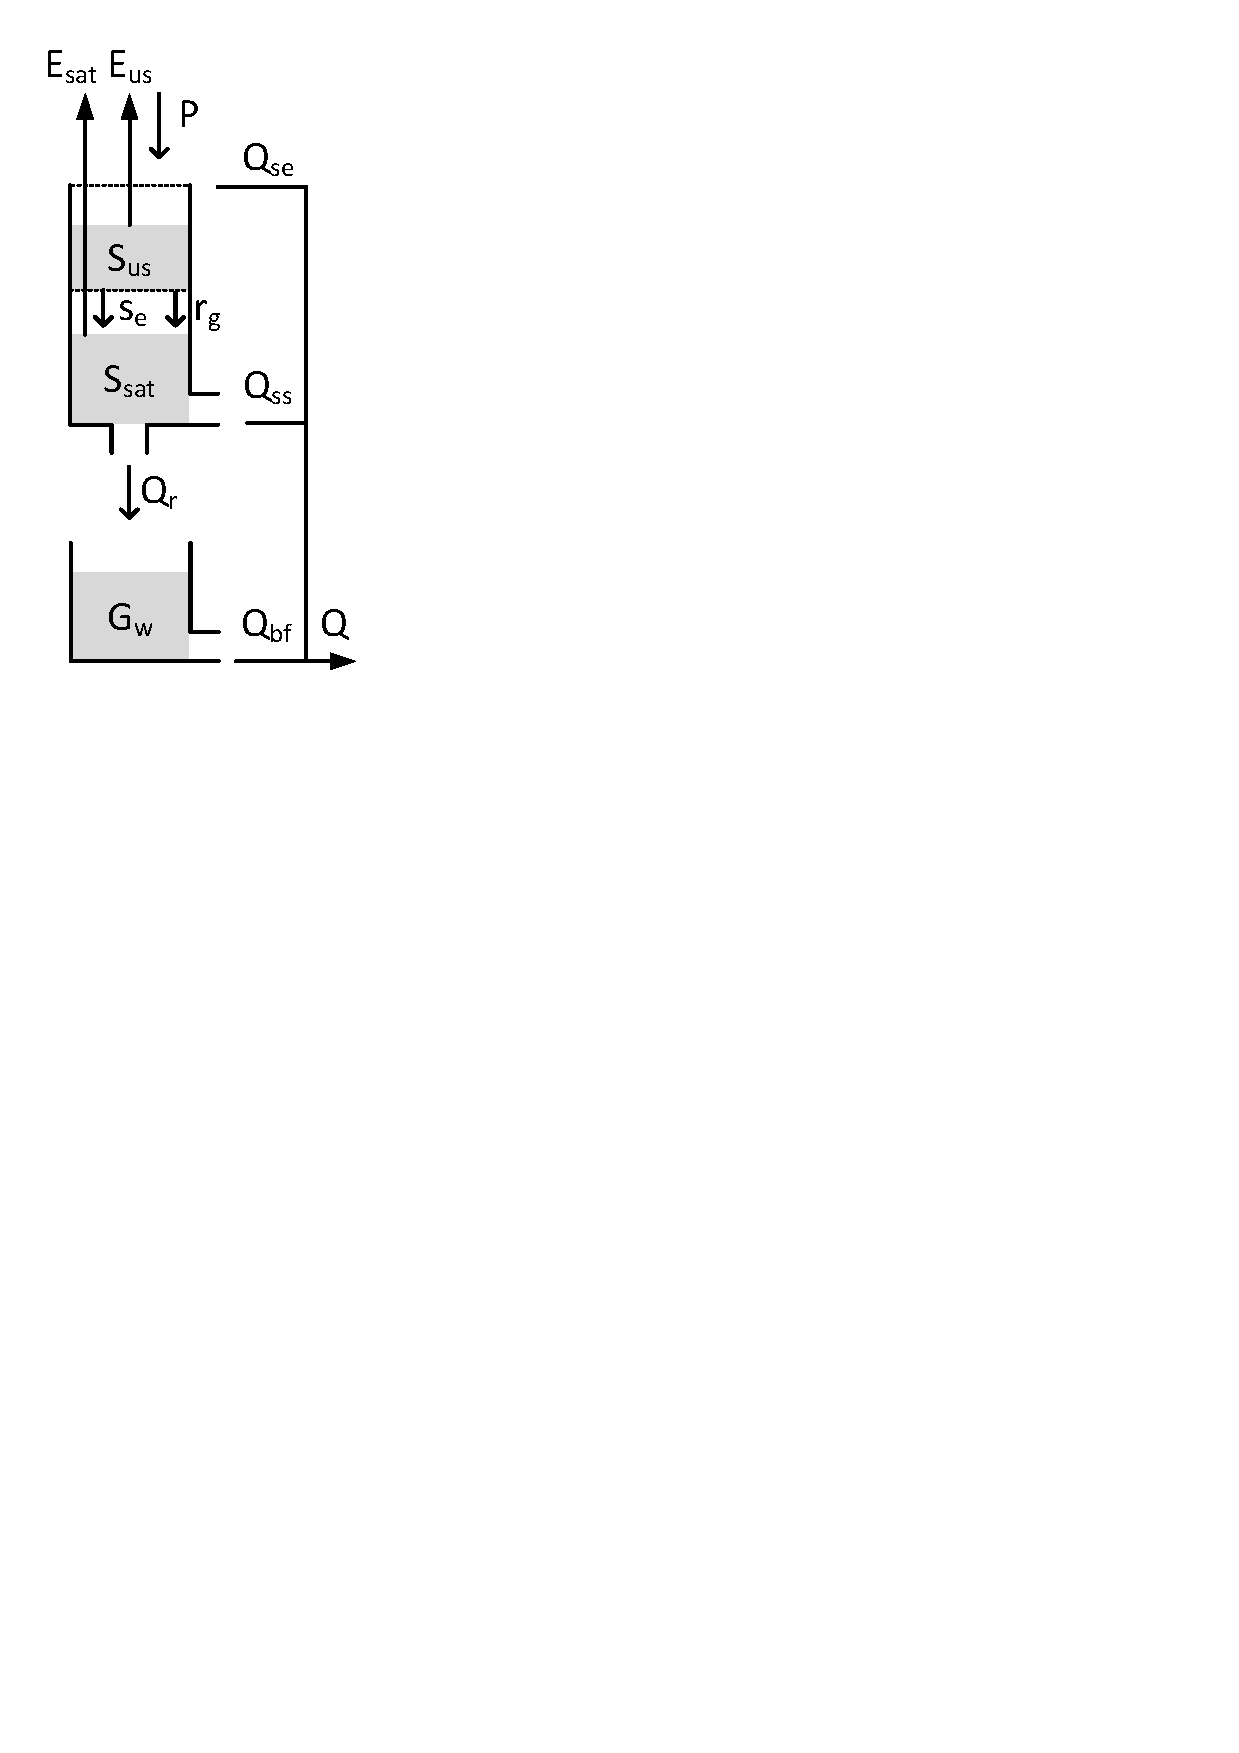
\includegraphics[trim=1cm 18cm 14cm 0.8cm,width=5cm,keepaspectratio]{./files/19_schematic.pdf}
\caption{Structure of the Australia model} \label{fig:19_schematic}
\end{wrapfigure}

\begin{align}
	\frac{dS_{us}}{dt} &= P-E_{us}-r_g -s_e\\
	E_{us} &= \frac{S_{us}}{S_b}*E_p\\
	S_b &= D*\phi\\
	r_g &= 
	\begin{cases}
		P, & if~S_{us} > S_{usfc}\\
		0, & \text{otherwise} \\
	\end{cases} \\
	s_e &= \begin{cases}
			S_{us} - S_{usfc}, & if~S_{us} > S_{usfc}\\
			0, & \text{otherwise} \\
			\end{cases}\\
	S_{usfc} &= (S_b - S_{sat})*\frac{fc}{\phi} 
\end{align}

Where $S_{us}$ is the current storage in the unsaturated store [mm], $P$ the current precipitation $[mm/d]$, $S_b$ [mm] the maximum storage of the soil profile, based on the soil depth $D$ [mm] and the porosity $\phi$ [-]. $r_g$ $[mm/d]$ is drainage from the unsaturated store to the saturated store, based on the variable field capacity $S_{usfc}$ [mm]. $S_{usfc}$ is based on the current storage on the saturated zone $S_{sat}$ [mm], the maximum soil moisture storage $S_b$ [mm], the field capacity $fc$ [-] and the porosity $\phi$ [-]. $s_e$ $[mm/d]$ is the storage excess, resulting from a decrease of $S_{usfc}$ that leads to more water being stored in the unsaturated zone than should be possible.

} % end wrap

\begin{align}
	\frac{dS_{sat}}{dt} &= r_g - E_{sat} - Q_{SE} - Q_{SS} - Q_{R}\\
	E_{sat} &= \frac{S_{sat}}{S_b}*E_p\\
	Q_{SE} &= \begin{cases}
		r_g+S_e, &\text{if } S_{sat} > S_b \\
		0, & \text{otherwise} \\
	\end{cases} \\
	Q_{SS} &= \alpha_{SS}*\left(S_{sat}\right)^{\beta_{SS}}\\
	Q_{R} &= K_{deep}*S_{sat}
\end{align}

Where $S_{sat}$ is the current storage in the saturated zone [mm], $E_{sat}$ is the evaporation from the saturated zone [mm], $Q_{SE}$ saturation excess runoff $[mm/d]$ that occurs when the saturated zone reaches maximum capacity $S_b$ [mm], $Q_{SS}$ is subsurface flow $[mm/d]$ and $Q_R$ is recharge of deep groundwater $[mm/d]$. Both $Q_{SS}$ and $Q_R$ are based on the dimensionless fraction $r$ and subsurface flow constants $c$ $[d^{-1}]$ and $d$ [-]. 

\begin{align}
	\frac{dG_w}{dt} &= Q_{R} - Q_{BF}\\
	Q_{BF} &= \alpha_{BF}*\left(G_w\right)^{\beta_{BF}}\\
\end{align}

Where $G_w$ is the current groundwater storage [mm] and $Q_{BF}$ baseflow, dependent on parameters  $\alpha_{BF}$ $[d^{-1}]$ and $\beta_{BF}$ [-]. Total runoff is the sum of $Q{SE}$, $Q_{SS}$ and $Q_{BF}$:

\begin{align}
	Q &= Q_{SE} + Q_{SS} + Q_{BF}
\end{align}

\newpage
\subsubsection{Parameter overview}
% Table generated by Excel2LaTeX from sheet 'Sheet1'
\begin{table}[htbp]
  \centering
    \begin{tabular}{lll}
    \toprule
    Parameter & Unit  & Description \\
    \midrule
    $S_b$ & $mm$  & Maximum soil moisture storage \\
    $\phi$ & $-$   & Porosity \\
    $fc$  & $-$   & Field capacity \\
    $\alpha_{SS}$ & $d^{-1}$ & Runoff coefficient \\
    $\beta_{SS}$ & $-$   & Runoff nonlinearity \\
    $K_{deep}$ & $d^{-1}$ & Runoff coefficient \\
    $\alpha_{BF}$ & $d^{-1}$ & Runoff coefficient \\
    $\beta_{BF}$ & $-$   & Runoff nonlinearity \\
    \bottomrule
    \end{tabular}%
  \label{tab:addlabel}%
\end{table}%


\section{Generalized Surface inFiltration Baseflow model (model ID: 20)}
The GSFB model (fig.~\ref{fig:20_schematic}) is  originally developed for use in Australian ephemeral catchments \citep{Nathan1990,Ye1997}. It has 3 stores and 8 parameters ($C$, $NDC$, $S_{max}$, $E_{max}$, $F_{rate}$, $B$, $DPF$ and $SDR_{max}$). The model aims to represent:

\begin{itemizecompact}
\item Saturation excess surface runoff;
\item Threshold-based infiltration;
\item Threshold-based baseflow;
\item Deep percolation and water rise to meet evaporation demand.
\end{itemizecompact}

\subsection{MARRMoT model name}
m\_20\_gsfb\_8p\_3s \\

% Equations
\subsection{Model equations}

% Model layout figure
{ 																	% This ensures it doesn't warp text further down
\begin{wrapfigure}{l}{4.5cm}
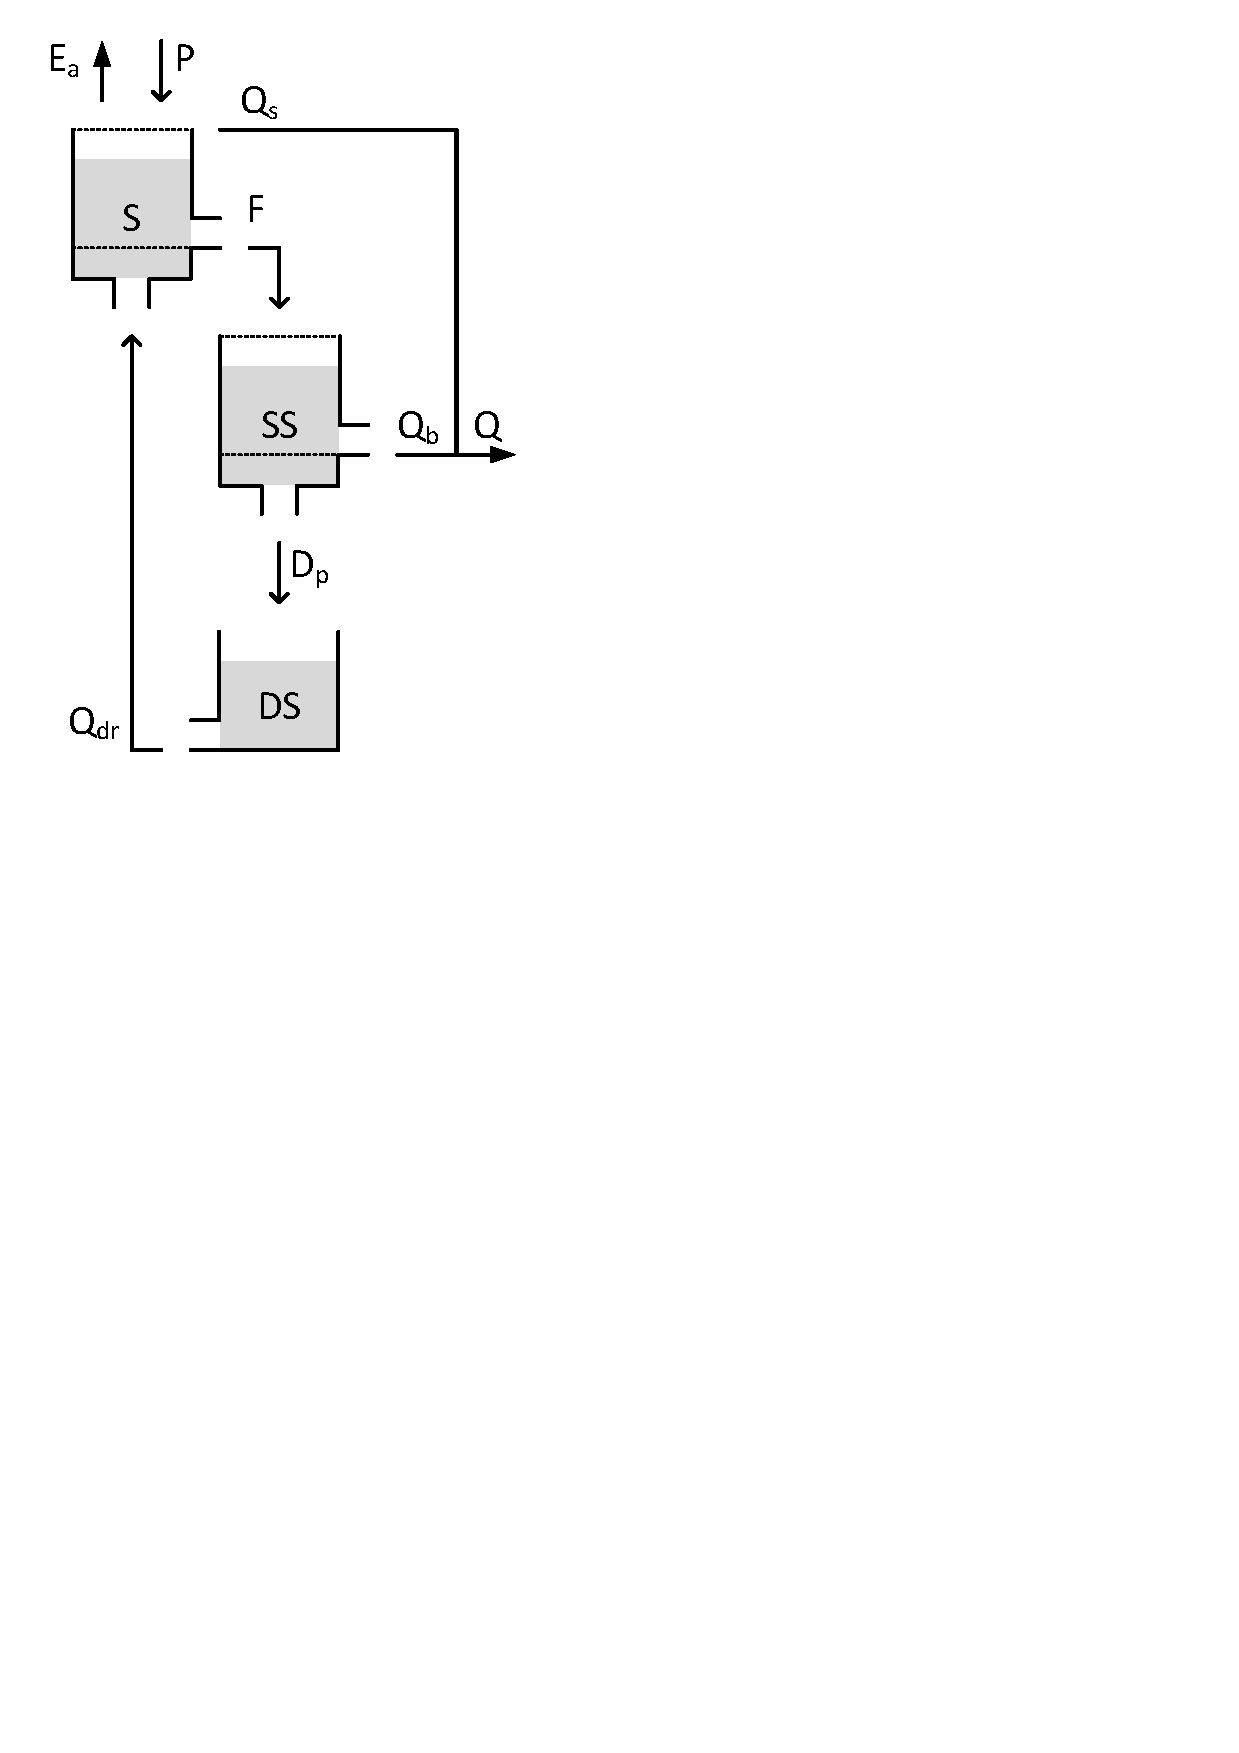
\includegraphics[trim=1cm 17cm 7cm 1cm,width=7cm,keepaspectratio]{./AppA_files/20_schematic.pdf}
\caption{Structure of the GSFB model} \label{fig:20_schematic}
\end{wrapfigure}

\begin{align}
	\frac{dS}{dt} &= P + Q_{dr}- E_a -Q_s-F \\
	Q_{dr} &= \begin{cases}
		C*DS*\left(1-\frac{S}{NDC*S_{max}}\right), &\text{if } S \leq NDC*S_{max} \\
		0, & \text{otherwise} \\
	\end{cases} \\
	E_a &= 
	\begin{cases}
		E_p, & \text{if } S > NDC*S_{max} \\
		min\left(E_p, E_{max}\frac{S}{NDC*S_{max}}\right), & \text{otherwise}
	\end{cases} \\
	Q_s &= \begin{cases}
		P, &\text{if } S = S_{max} \\
		0, & \text{otherwise} \\
	\end{cases} \\
	F &= \begin{cases}
		F_{rate}, &\text{if } S > NDC*S_{max} \\
		0, & \text{otherwise} \\
	\end{cases} 
\end{align}

} % end of wrapfigure fix
\vspace{1cm}

Where $S$ [mm] is the current storage in the upper zone, refilled by precipitation $P$ $[mm/d]$ and recharge from deep groundwater $Q_{dr}$ $[mm/d]$. 
The store is drained by evaporation $E_a$ $[mm/d]$, surface runoff $Q_{s}$ $[mm/d]$ and infiltration $F$ $[mm/d]$.
$E_a$ occurs at the potential rate $E_p$ $[mm/d]$ if the store is above a threshold capacity given as the fraction $NDC$ [-] of maximum storage $S_{max}$ [mm].
Evaporation occurs at a reduced rate scaled by maximum evaporation rate $E_{max}$ $[mm/d]$ if the store is below this threshold.
$Q_s$ occurs only if the store is at maximum capacity $S_{max}$. 
$F$ occurs at a constant rate $F_{rate}$ if the store is above threshold $NDC*S_{max}$.
Recharge from deep percolation only occurs if the store is below threshold capacity $NDC*S_{max}$ and uses time parameter $C$ $[d^{-1}]$ and current deep storage $DS$ [mm].

\begin{align}
	\frac{dSS}{dt} &=F - Q_b-D_p\\
	Q_b &= \begin{cases}
		B*DPF*(SS-SDR_{max}), &\text{if } SS > SDR_{max} \\
		0, & \text{otherwise} \\
	\end{cases} \\
	D_p &= (1-B)*DPF*SS
\end{align}

Where $SS$ [mm] is the current storage in the subsurface store, refilled by infiltration $F$ and drained by baseflow $Q_b$ $[mm/d]$ and deep percolation $D_p$ $[mm/d]$.
Outflow from this store is given as a function of storage $DS$ and time coefficient  $DPF$ $[d^{-1}]$.
A fraction $1-B$ [-] of this outflow is deep percolation $D_p$.
The remaining fraction $B$ [-] is baseflow $Q_b$, provided the store is above threshold $SDR_{max}$ [mm].

\begin{align}
	\frac{dDS}{dt} &= D_p - Q_{dr}  \\
\end{align}
  
Where $DS$ [mm] is the current storage in the deep store, refilled by a deep percolation $D_p$ and drained by recharge to the upper store $Q_{dr}$.
Total flow:

\begin{align}
	Q_t &= Q_s+Q_b
\end{align}

\subsection{Parameter overview}

% Table generated by Excel2LaTeX from sheet 'Sheet1'
\begin{table}[htbp]
  \centering
    \begin{tabular}{lll}
    \toprule
    Parameter & Unit  & Description \\
    \midrule
    $C$   & $d^{-1}$ & Recharge coefficient \\
    $NDC$ & $-$   & Threshold for evaporation and recharge as fraction of $S_{max}$ \\
    $S_{max}$ & $mm$  & Maximum soil moisture storage \\
    $E_{max}$ & $mm~d^{-1}$ & Maximum evaporation rate \\
    $F_{rate}$ & $mm~d^{-1}$ & Recharge rate \\
    $B$   & $-$   & Fraction subsurface flow to stream \\
    $DPF$ & $d^{-1}$ & Runoff coefficient \\
    $SDR_{max}$ & $mm$  & Threshold for subsurface flow generation \\
    \bottomrule
    \end{tabular}%
  \label{tab:addlabel}%
\end{table}%

\section{Flex-B (model ID: 21)}
The Flex-B model (fig.~\ref{fig:21_schematic}) is the basis of a model development study \citep{Fenicia2008}. It has 3 stores and 9 parameters ($UR_{max}$, $\beta$, $D$, $Perc_{max}$, $L_p$, $N_{lag,f}$, $N_{lag,s}$, $K_f$ and $K_s$). The model aims to represent:

\begin{itemizecompact}
\item Infiltration and saturation excess flow based on a distribution of different soil depths;
\item A split between fast saturation excess flow and preferential recharge to a slow store;
\item Percolation from the unsaturated zone to a slow runoff store.
\end{itemizecompact}

\subsection{MARRMoT model name}
m\_21\_flexb\_9p\_3s \\

% Equations
\subsection{Model equations}

% Model layout figure
{ 																	% This ensures it doesn't warp text further down
\begin{wrapfigure}{l}{7cm}
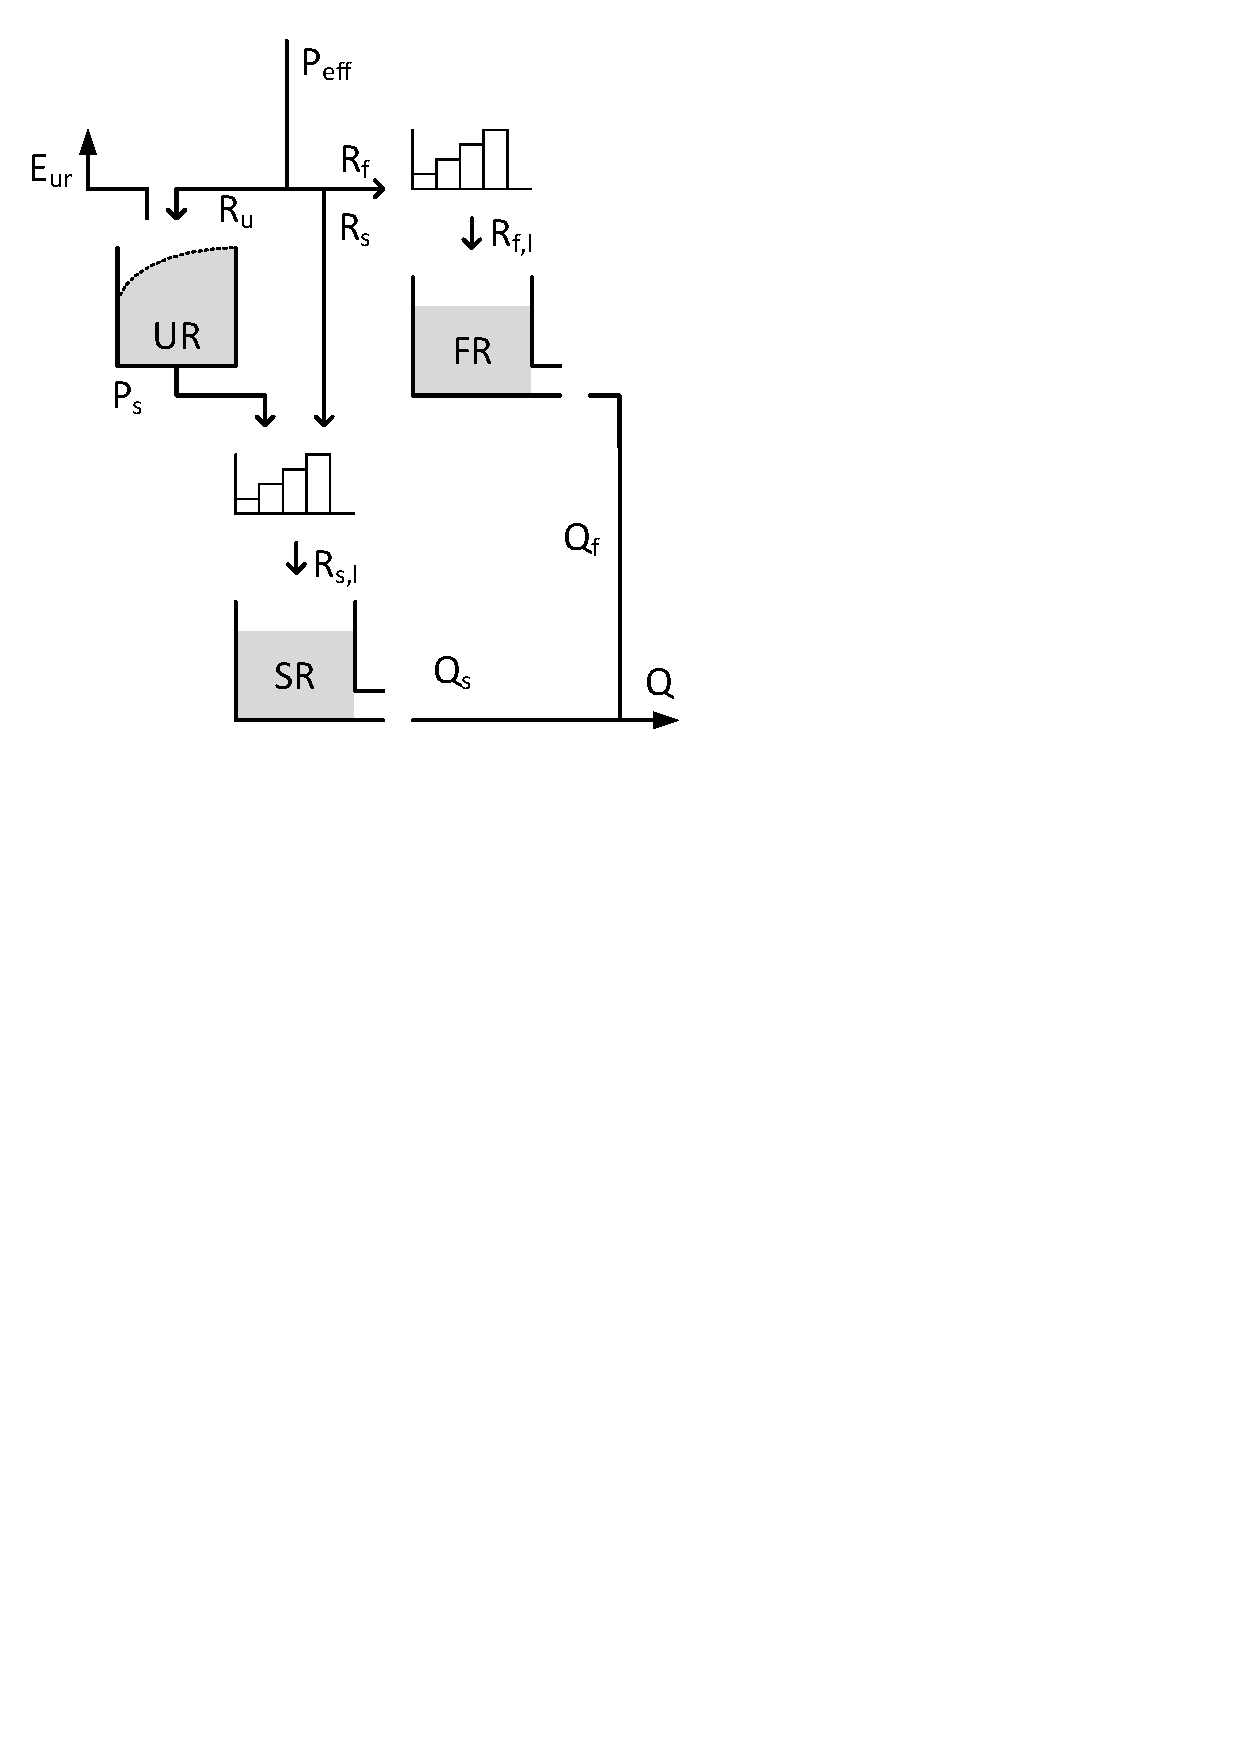
\includegraphics[trim=1cm 17.5cm 7cm 1cm,width=7cm,keepaspectratio]{./AppA_files/21_schematic.pdf}
\caption{Structure of the Flex-B model} \label{fig:21_schematic}
\end{wrapfigure}

\begin{align}
	\frac{dUR}{dt} &= R_u - E_{ur} - R_p \\
	R_U &= (1 - C_r) * P_{eff}\\
	C_r &= \Big[1+exp\Big(\frac{-UR/UR_{max} + 1/2}{\beta}\Big)\Big]^{-1}\\
	%R_u &= (1 - \Big[1+exp\Big(\frac{-UR/UR_{max} + 1/2}{\beta}\Big)\Big]^{-1}) * P_{eff}\\
	E_{ur} &= E_p * min\Big(1, \frac{UR}{UR_{max}} \frac{1}{L_p}\Big)\\
	P_s&= Perc_{max} * \frac{UR}{UR_{max}}
\end{align}
  
Where UR is the current storage in the unsaturated zone [mm]. $R_u$ $[mm/d]$ is the inflow into UR based on its current storage compared to maximum storage $UR_{max}$ [mm] and a shape distribution parameter $\beta$ [-]. 

} % end of wrapfigure fix

$E_{ur}$ the evaporation $[mm/d]$ from UR which follows a linear relation between current and maximum storage until a threshold $L_p$ [-] is exceeded. $P_s$ is the percolation from UR to the slow reservoir SR $[mm/d]$, based on a maximum percolation rate $Perc_{max}$ [mm/d], relative to the fraction of current storage and maximum storage. $P_{eff}$ is routed towards the unsaturated zone based on $Cr$, with the remainder being divided into preferential recharge $R_s$ $[mm/d]$ and fast runoff $R_f$ $[mm/d]$:

\begin{align}
	R_s &= (P_{eff} - R_u)*D\\
	R_f &= (P_{eff} - R_u)*(1-D)
\end{align}

Where $R_s$ and $R_f$ are the flows $[mm/d]$ to the slow and fast runoff reservoir respectively, based on runoff partitioning coefficient D [-]. Both are lagged by linearly increasing triangular transformation functions with parameters $N_{lag,s}$ [d] and $N_{lag,f}$ [d] respectively. Percolation $R_p$ is added to $R_s$ before the transformation to $R_{s,l}$ occurs.

\begin{align}
	\frac{dFR}{dt} &= R_{f,l} - Q_f\\
	Q_f &= K_f * FR 
\end{align}

Where FR is the current storage [mm] in the fast flow reservoir. Outflow $Q_f$ $[mm/d]$ from the reservoir has a linear relation with storage through time scale parameter $K_f$ [$d^{-1}$]. 

\begin{align}
	\frac{dSR}{dt} &= R_{s,l} - Q_s \\
	Q_s &= K_s * SR 
\end{align}

Where SR is the current storage [mm] in the slow flow reservoir. Outflow $Q_s$ $[mm/d]$ from the reservoir has a linear relation with storage through time scale parameter $K_s$ [$d^{-1}$]. Total outflow Q  $[mm/d]$:

\begin{equation}
	Q = Q_f + Q_s
\end{equation}

\subsection{Parameter overview}
% Table generated by Excel2LaTeX from sheet 'Sheet1'
\begin{table}[htbp]
  \centering
    \begin{tabular}{lll}
    \toprule
    Parameter & Unit  & Description \\
    \midrule
    $UR_{max}$ & $mm$  & Maximum soil moisture storage \\
    $\beta$ & $-$   & Shape parameter \\
    $D$   & $-$   & Fraction effective precipitation to slow store \\
    $Perc_{max}$ & $mm~d^{-1}$ & Maximum percolation rate \\
    $L_p$ & $-$   & Wilting point as fraction of $UR_{max}$ \\
    $N_{lag,f}$ & $d$   & Unit Hydrograph time base \\
    $N_{lag,s}$ & $d$   & Unit Hydrograph time base \\
    $K_f$ & $d^{-1}$ & Runoff coefficient \\
    $K_s$ & $d^{-1}$ & Runoff coefficient \\
    \bottomrule
    \end{tabular}%
  \label{tab:addlabel}%
\end{table}%

\subsection{Variable Infiltration Capacity (VIC) model (model ID: 22)}
The VIC model (fig.~\ref{fig:22_schematic}) is originally developed for use with General Circulation Models and uses latent and sensible heat fluxes to determine the rainfall-runoff relationship \citep{Liang1994}. For consistency with other models in this framework, we use a conceptualized version based in part of the VIC implementation in \citet{Clark2008a}. In addition, the original Leaf-Area-Index-based interception capacity is replaced with a sinusoidal curve-based approximation of interception capacity. The model has 3 stores and 10 parameters ($\bar{I}$, $I_{\delta}$, $I_s$, $S_{sm,max}$, $b$, $k_1$, $c_1$, $S_{gw,max}$, $k_2$ and $c_2$). The model aims to represent:

\begin{itemizecompact}
\item Time-varying interception by vegetation;
\item Variable infiltration and saturation excess flow;
\item Interflow and baseflow from a deeper groundwater layer.
\end{itemizecompact}

\subsubsection{File names}
\begin{tabular}{@{}ll}
Model: &m\_22\_vic\_10p\_3s \\
Parameter ranges: &m\_22\_vic\_10p\_3s\_parameter\_ ranges \\
\end{tabular}

% Equations
\subsubsection{Model equations}

% Model layout figure
{ 																	% This ensures it doesn't warp text further down
\begin{wrapfigure}{l}{3cm}
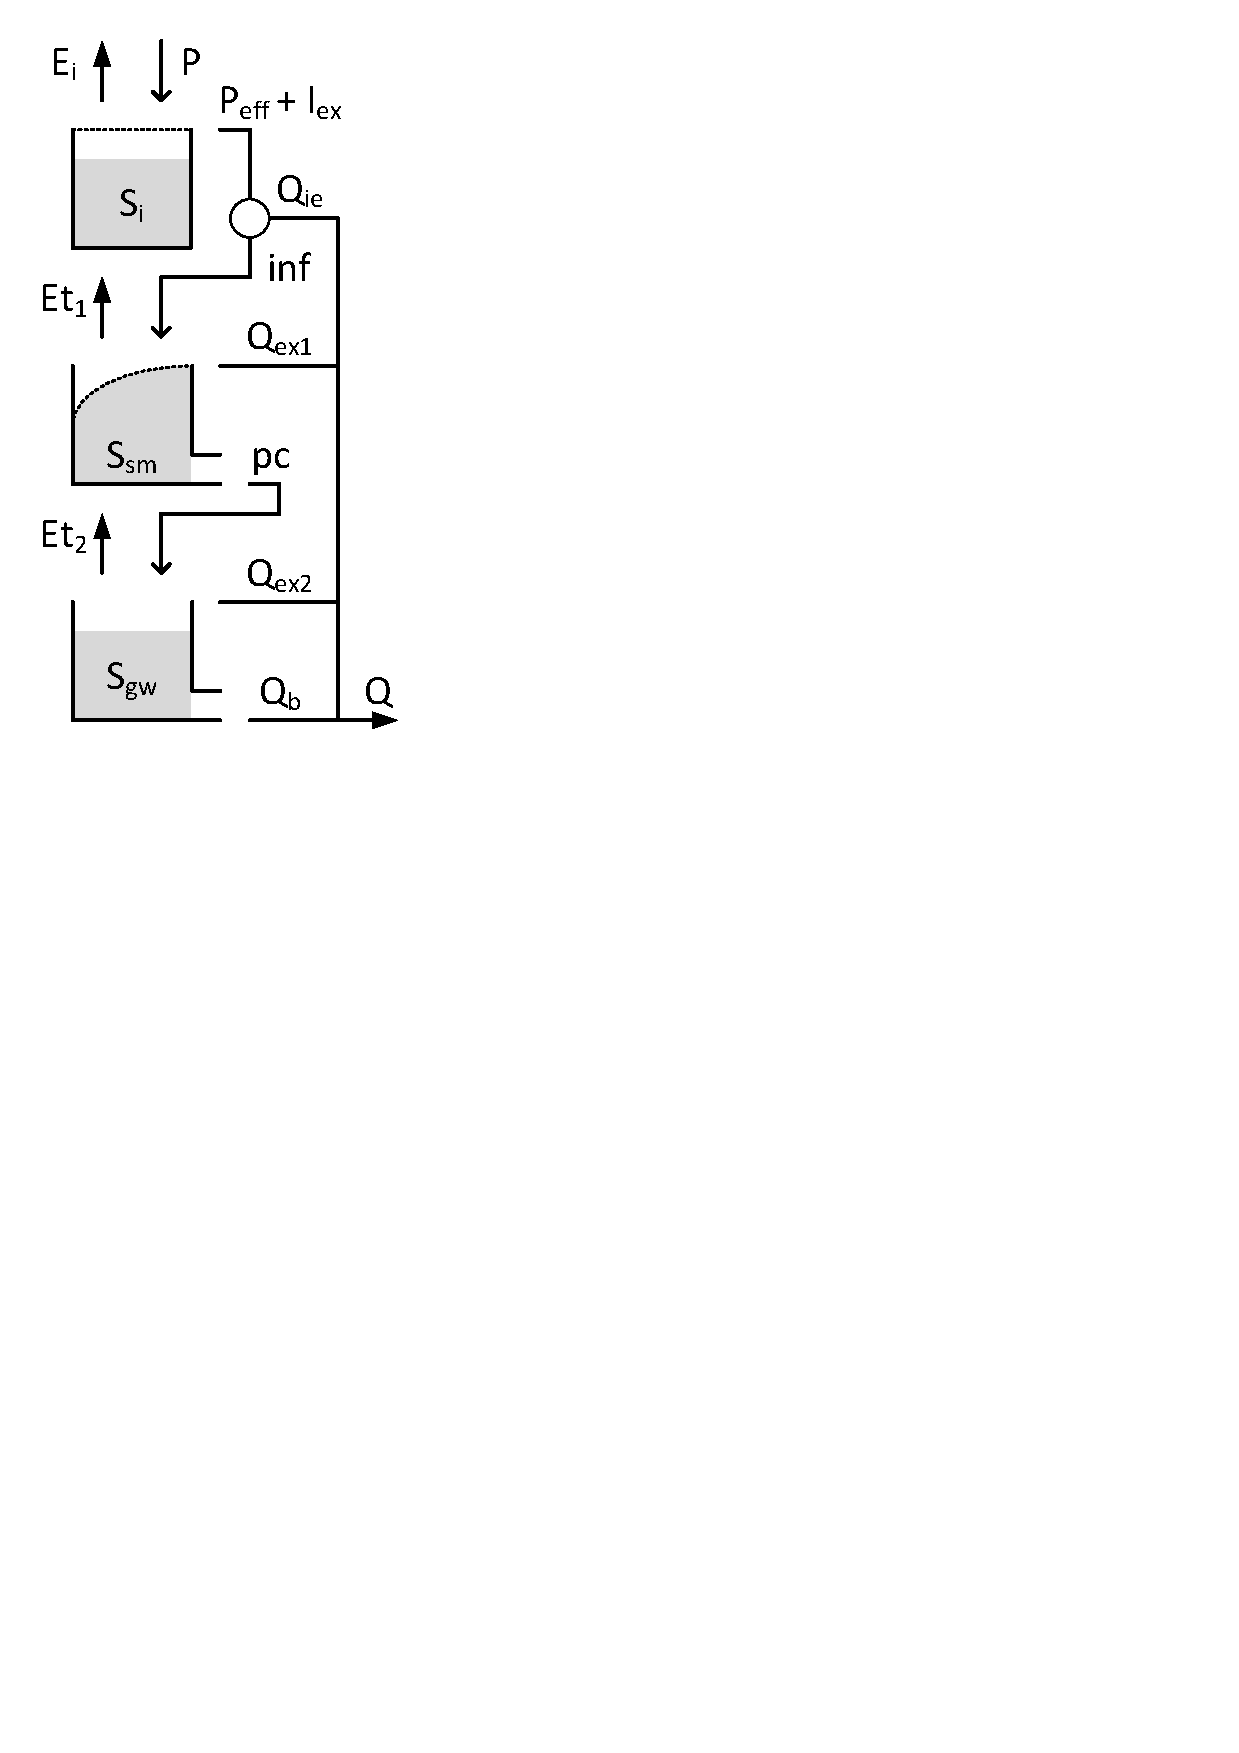
\includegraphics[trim=1cm 17cm 7cm 1cm,width=7cm,keepaspectratio]{./files/22_schematic.pdf}
\caption{Structure of the VIC model} \label{fig:22_schematic}
\end{wrapfigure}

\begin{align}
	\frac{dS_i}{dt} &= P - E_i - P_{eff} - I_{ex} \\
	E_i &= \frac{S_i}{I_{max}}*E_p \\
	I_{max} &= \bar{I}\left(1+I_{\delta}*sin\left(2\pi(t+I_s)\right)\right)\\
	P_eff &=\begin{cases}
		P, & \text{if }S_i = I_{max} \\
		0, & \text{otherwise}\\
	\end{cases}\\
	I_{ex} &= max\left(S_i - I_{max}\right)
\end{align}

Where $S_i$ [mm] is the current interception storage, refilled by precipitation P $[mm/d]$ and drained by evaporation $E_i$ $[mm/d]$ and interception excess flows $P_{eff}$$[mm/d]$ and $I_{ex}$ $[mm/d]$. $E_i$ decreases linearly with storage, based on maximum storage $I_{max}$ [mm]. $I_{max}$ is determined using the mean interception $\bar{I}$ [mm], fractional seasonal interception change $I_{\delta}$ [-] and time shift $I_s$ [d]. It is implicitly assumed that 1 sinusoidal period corresponds with a growing season of 1 year. $P_{eff}$ is effective rainfall when the store is at maximum capacity. $I_{ex}$ is an auxiliary flux used when a change in storage size result in current storage $S_i$ exceeding $I_{max}$.

} % end of wrapfigure fix

\begin{align}
	\frac{dS_{sm}}{dt} &= inf-Et_1-Q_{ex1}-pc\\
	inf &= \left(P_{eff}+I_{ex}\right) - Q_{ie} \\
	Q_{ie} &= \left(P_{eff}+I_{ex}\right)*\left(1-\left(1-\frac{S_{sm}}{S_{sm,max}}\right)^b\right)\\
	E_{t1} &= \frac{S_{sm}}{S_{sm,max}}*(E_p-E_i)\\
	Q_{ex1} &= \begin{cases}
		inf, &\text{if }S_{sm} = S_{sm,max}\\
		0, &\text{otherwise}\\
	\end{cases}	\\
	pc &= k_1*\left(\frac{S_{sm}}{S_{sm,max}}\right)^{c_1}
\end{align}

Where $S_{sm}$ [mm] is the current soil moisture storage, refilled by infiltration $inf$  $[mm/d]$, and drained by evapotranspiration $Et_1$  $[mm/d]$, storage excess $Q_{ex1}$  $[mm/d]$ and percolation $pc$  $[mm/d]$. $inf$ relies on the value of infiltration excess $Q_{ie}$, which is calculated using the maximum soil moisture storage $S_{sm,max}$ [mm] and shape parameter $b$ [-]. $Et_1$ scales linearly with current storage. $Q_{ex1}$ equals $inf$ when the store is at maximum capacity. $pc$ has a potentially non-linear relationship with current storage through time parameter $k_1$ $[d^{-1}]$ and shape parameter $c_1$.

\begin{align}
	\frac{dS_{gw}}{dt} &= pc-Et_2-Q_{ex2}-Q_b\\
	Et_2 &= \frac{S_{gw}}{S_{gw,max}}*\left(E_p-E_i-Et_1\right)\\
	Q_{ex2} &= \begin{cases}
		pc, &\text{if }S_{gw} = S_{gw,max}\\
		0, &\text{otherwise}\\
	\end{cases}	\\
	Q_b &=  k_2*\left(\frac{S_{gw}}{S_{gw,max}}\right)^{c_2}
\end{align}

Where $S_{gw}$ [mm] is the current groundwater storage, refilled through percolation $pc$ $[mm/d]$ and drained by evapotranspiration $Et_2$ $[mm/d]$, excess flow $Q_{ex2}$ $[mm/d]$ and baseflow $Q_b$ $[mm/d]$. $Et_2$ is scaled linearly with current storage based on maximum storage $S_{gw,max}$ [mm]. $Q_{ex2}$ equals $pc$ when the store is at maximum capacity. $Q_b$ has a potentially non-linear relationship with current storage through time parameter $k_2$ and shape parameter $c_2$. Total outflow:

\begin{align}
	Q_t &= Q_{ie}+Q_{ex1}+Q_{ex2}+Q_b
\end{align}

\newpage
\subsubsection{Parameter overview}
% Table generated by Excel2LaTeX from sheet 'Sheet1'
\begin{table}[htbp]
  \centering
    \begin{tabular}{lll}
    \toprule
    Parameter & Unit  & Description \\
    \midrule
    $\bar{I}$ & $mm$  & Mean annual interception storage \\
    $I_{\delta}$ & $-$   & Seasonal interception change as fraction of $\bar{I}$ \\
    $I_s$ & $d$   & Time shift of maximum interception storage \\
    $S_{sm,max}$ & $mm$  & Maximum soil moisture storage \\
    $b$   & $-$   & Shape parameter \\
    $k_1$ & $d^{-1}$ & Runoff coefficient \\
    $c_1$ & $-$   & Runoff nonlinearity \\
    $S_{gw,max}$ & $mm$  & Maximum groundwater storage \\
    $k_2$ & $d^{-1}$ & Runoff coefficient \\
    $c_2$ & $-$   & Runoff nonlinearity \\
    \bottomrule
    \end{tabular}%
  \label{tab:addlabel}%
\end{table}%

\section{Large-scale catchment water and salt balance model element (model ID: 23)}
The large-scale catchment water and salt balance model (LASCAM) (fig.~\ref{fig:23_schematic}) is part of a study that investigates soil water and salt concentration before and after forest clearing \citep{Sivapalan1996a}. It is a semi-distributed model made up of individual elements, such as described below. The model presented here simulates the water balance only (salt is ignored). It has 3 stores and 24 parameters ($\alpha_f$, $\beta_f$, $B_{max}$,  $F_{max}$, $\alpha_c$, $\beta_c$, $A_{min}$, $A_{max}$, $\alpha_{ss}$, $\beta_{ss}$, $c$, $\alpha_g$, $\beta_g$, $\gamma_f$, $\delta_f$, $t_d$, $\alpha_b$, $\beta_b$, $\gamma_a$, $\delta_a$, $\alpha_a$, $\beta_a$, $\gamma_b$ and $\delta_b$). The model aims to represent:

\begin{itemizecompact}
\item Stylized interception;
\item Saturation and infiltration excess surface runoff;
\item An inner layout representing near-stream saturated storage, deep saturated storage and medium-depth unsaturated storage;
\item Subsurface saturation and infiltration excess flow to the near-stream store;
\item Percolation to and capillary rise from groundwater.
\end{itemizecompact}

\subsection{MARRMoT model name}
m\_23\_lascam\_24p\_3s \\

% Equations
\subsection{Model equations}

% Model layout figure
{ 																	% This ensures it doesn't warp text further down
\begin{wrapfigure}{l}{5cm}
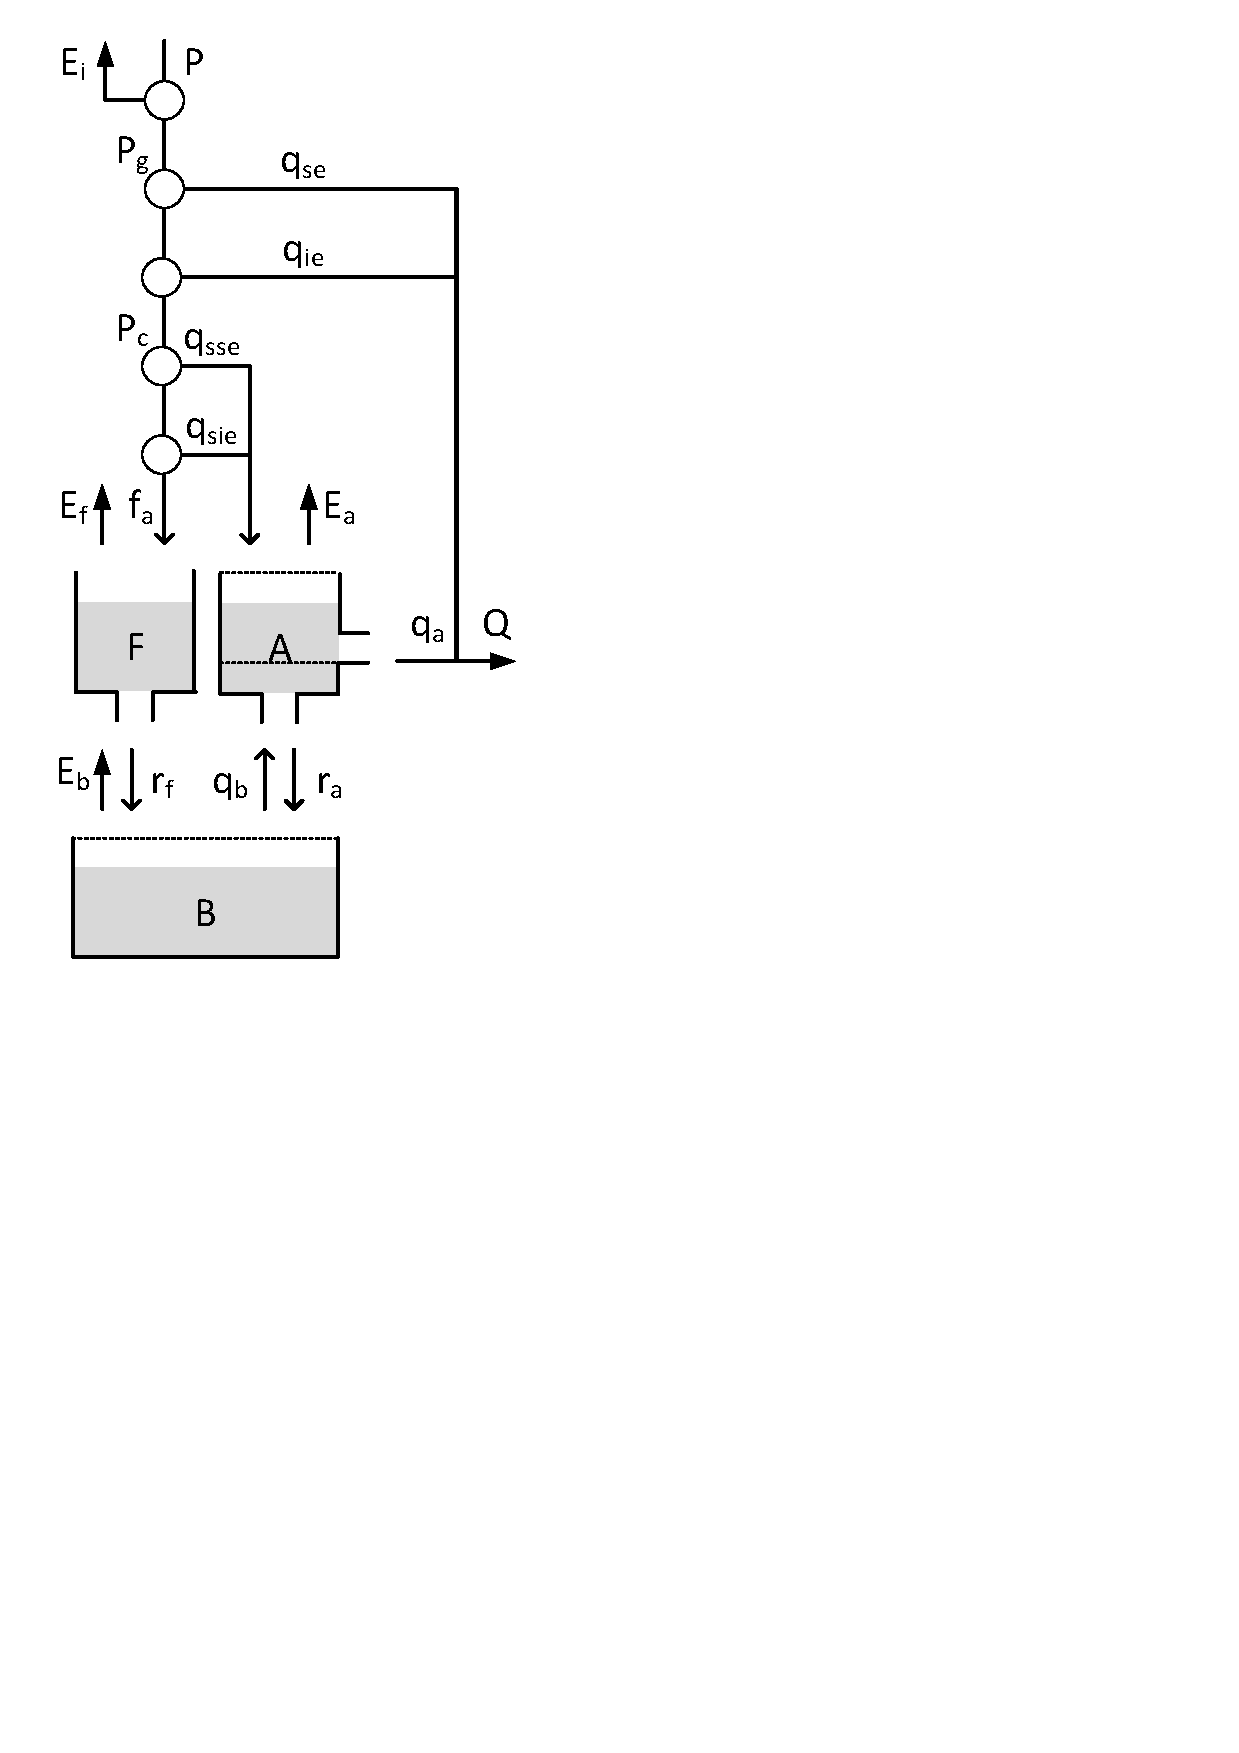
\includegraphics[trim=1cm 13.5cm 7cm 1cm,width=7cm,keepaspectratio]{./AppA_files/23_schematic.pdf}
\caption{Structure of the LASCAM model} \label{fig:23_schematic}
\end{wrapfigure}

\begin{align}
	\frac{dF}{dt} &= f_a-E_f-r_f \\
	f_a &= min\left(P_c*max\left(1,\frac{1-\phi_{ss}}{1-\phi_c}\right),f_{ss}^*\right) \\
	f_{ss}^* &= \alpha_f\left(1-\frac{B}{B_{max}}\right)\left(\frac{F}{F_{max}}\right)^{-\beta_f}\\
	\phi_c &= \begin{cases}
		\alpha_c\left(\frac{A-A_{min}}{A_{max}-A_{min}}\right)^{\beta_c}, &\text{if } A > A_{min} \\
		0, & \text{otherwise} \\
	\end{cases}\\
	\phi_{ss} &= \begin{cases}
		\alpha_{ss}\left(\frac{A-A_{min}}{A_{max}-A_{min}}\right)^{\beta_{ss}}, &\text{if } A > A_{min} \\
		0, & \text{otherwise} \\
	\end{cases}\\
	P_c &= min\left(P_g-q_{se},f^*_s\right) \\
	f^*_s &= c \\
	q_{se} &= \phi_c*P_g \\
	P_g &= max\left(\alpha_g+\beta_g*P,0\right)\\
	E_f &= \gamma_f*E_p\left(\frac{F}{F_{max}}\right)^{\delta_f}\\
	r_f &= t_d*F
\end{align}

} % end of wrapfigure fix

Where $F$ [mm] is the current storage in the unsaturated infiltration store, which controls the amount of subsurface runoff generated on the boundary of a more permeable top layer (store $A$) with a less permeable bottom layer (store $F$).
$F$ is refilled by actual infiltration $f_a$ $[mm/d]$, and drained by recharge $r_f$ $[mm/d]$ and evaporation $E_b$ $[mm/d]$. 
$f_a$ depends on the actual infiltration rate $P_c$ $[mm/d]$, the fraction saturated catchment area $\phi_{ss}$ [-], the fraction variable area contributing to overland flow $\phi_c$ [-] and a catchment-scale infiltration capacity $f_{ss}^*$ $[mm/d]$. 
$f_{ss}^*$ depends on a scaling parameter $\alpha_f$ $[mm/d]$, the relative storage in groundwater $B/B_{max}$, the relative infiltration volume in the catchment $F/F_{max}$ and non-linearity parameter $\beta_f$ [-]. 
$B_{max}$ [mm] and $F_{max}$ [mm] are storage scaling parameters [-].
$\phi_c$ uses the minimum contributing storage $A_{min}$ [mm], maximum contributing storage $A_{max}$ [mm] and shape parameters $\alpha_c$ [-] and $\beta_c$ [-] to control the shape of this distribution.
$\phi_{ss}$ takes a similar shape as $\phi_c$, using parameters $\alpha_{ss}$ [-] and $\beta_{ss}$ [-].
$P_c$ is the lesser of throughfall rate $P_g$  $[mm/d]$ minus saturation excess $q_{se}$  $[mm/d]$, and the catchment infiltration capacity $f_s^*$  $[mm/d]$.
$f_s^*$ is assumed to have a constant rate $c$  $[mm/d]$.
$q_{se}$ is determined as that part of throughfall $P_g$ that falls on the variable contributing catchment area given by $\phi_c$.
$P_g$ is determined as a fixed interception rate $\alpha_g$  $[mm/d]$ and a fractional interception $\beta_g$ [-].
Evaporation $E_f$ uses the potential rate $E_p$ $[mm/d]$  scaled by the relative storage in $F$ and two shape parameters  $\gamma_f$ [-]  and $\delta_f$ [-].
Recharge $r_f$ $[mm/d]$ has a linear relation with storage through time parameter $t_d$ $[d^{-1}]$.

\begin{align}
	\frac{dA}{dt} &= q_{sse} +q_{sie} + q_b - E_a - q_a - r_a\\
	q_{sse} &= \frac{\phi_{ss}-\phi_c}{1-\phi_c}P_c\\
	q_{sie} &= max\left(P_c*\frac{1-\phi_{ss}}{1-\phi_c}-f^*_{ss},0\right) \\
	q_b &= \beta_b\left(exp\left(\alpha_b\frac{B}{B_{max}}\right)-1\right) \\
	E_a &= \phi_c*E_p + \gamma_a*E_p\left(\frac{A}{A_{max}}\right)^{\delta_a}\\
	q_a &= \begin{cases}
		\alpha_a\left(\frac{A-A_{min}}{A_{max}-A_{min}}\right)^{\beta_a}, &\text{if } A > A_{min} \\
		0, & \text{otherwise} \\
	\end{cases}\\
	r_a &= \phi_{ss}*f^*_{ss}
\end{align}

Where $A$ [mm] is the current storage in the more permeable upper zone (above less permeable lower zone $F$), refilled by sub-surface saturation excess $q_{sse}$ $[mm/d]$, sub-surface infiltration excess $q_{sie}$ $[mm/d]$ and discharge from groundwater $q_b$ $[mm/d]$. 
The store is drained by evaporation $E_a$, subsurface stormflow $q_a$ $[mm/d]$ and recharge $r_a$ $[mm/d]$.
Flow from store $B$, $q_b$, decreases exponentially as the store dries out, controlled by parameters $\beta_b$ $[mm/d]$ and $\alpha_b$ [-]. 
Evaporation $E_a$ occurs at the potential rate $E_p$ from the variable saturated area $\phi_c$ and additionally at a rate scaled by the relative storage in $A$ and two shape parameters $\gamma_a$ [-] and $\delta_a$ [-].
Subsurface flow $q_a$ occurs only if current storage exceeds threshold $A_{min}$ and maximum rate $\alpha_a$ [mm/d], controlled by scaling parameter $\beta_a$ [-].
Recharge $r_a$ is a function of the saturated subsurface area $\phi_{ss}$ and the subsurface infiltration rate $f_{ss}^*$.

\begin{align}
	\frac{dB}{dt} &= r_f+r_a - E_b - q_b \\
	E_b &= \gamma_b*E_p\left(\frac{B}{B_{max}}\right)^{\delta_b}
\end{align}
  
Where $B$ [mm] is the current storage in the deep layers, refilled by recharge from stores A ($r_a$) and F ($r_f$), and drained by evaporation $E_b$ and groundwater discharge $q_b$.
$E_b$ uses the potential rate $E_p$ scaled by the relative storage in $B$ and two shape parameters $\gamma_b$ [-] and $\delta_b$ [-].
Total flow:

\begin{align}
	Q_t &=q_{se}+q_{ie}+q_a \\
	q_{ie} &= P_g-q_{se}-P_c
\end{align}

Where $q_{ie}$  $[mm/d]$ is infiltration excess on the surface.

\newpage
\subsection{Parameter overview}

% Table generated by Excel2LaTeX from sheet 'Sheet1'
\begin{table}[htbp]
  \centering
    \begin{tabular}{lrl}
    \toprule
    Parameter & \multicolumn{1}{l}{Unit} & Description \\
    \midrule
    $\alpha_f$ & \multicolumn{1}{l}{$mm~d^{-1}$} & Infiltration scaling parameter \\
    $\beta_f$ & \multicolumn{1}{l}{$-$} & Infiltration scaling parameter \\
    $B_{max}$ & \multicolumn{1}{l}{$mm$} & Infiltration scaling parameter \\
    $F_{max}$ & \multicolumn{1}{l}{$mm$} & Infiltration scaling parameter \\
    $\alpha_c$ & \multicolumn{1}{l}{$-$} & Overland flow fraction \\
    $\beta_c$ & \multicolumn{1}{l}{$-$} & Overland flow shape parameter \\
    $A_{min}$ & \multicolumn{1}{l}{$mm$} & Minimum contributing storage \\
    $A_{max}$ & \multicolumn{1}{l}{$mm$} & Maximum contributing storage \\
    $\alpha_{ss}$ & \multicolumn{1}{l}{$-$} & Saturated area fraction \\
    $\beta_{ss}$ & \multicolumn{1}{l}{$-$} & Saturated area shape parameter parameter \\
    $c$   & \multicolumn{1}{l}{$mm~d^{-1}$} & Catchment infiltration capacity \\
    $\alpha_g$ & \multicolumn{1}{l}{$mm~d^{-1}$} & Constant interception rate \\
    $\beta_g$ & \multicolumn{1}{l}{$-$} & Interception fraction \\
    $\gamma_f$ & \multicolumn{1}{l}{$-$} & Evaporation shape parameter \\
    $\delta_f$ & \multicolumn{1}{l}{$-$} & Evaporation shape parameter \\
    $t_d$ & \multicolumn{1}{l}{$d^{-1}$} & Runoff coefficient \\
    $\alpha_b$ & \multicolumn{1}{l}{$-$} & Groundwater discharge shape parameter \\
    $\beta_b$ & \multicolumn{1}{l}{$mm~d^{-1}$} & Maximum groundwater recharge rate \\
    $\gamma_a$ & \multicolumn{1}{l}{$-$} & Evaporation scaling parameter \\
    $\delta_a$ & \multicolumn{1}{l}{$-$} & Evaporation nonlinearity \\
    $\alpha_a$ & \multicolumn{1}{l}{$mm~d^{-1}$} & Maximum subsurface flow rate \\
    $\beta_a$ & \multicolumn{1}{l}{$-$} & Subsurface flow nonlinearity  \\
    $\gamma_b$ &       & Evaporation scaling parameter \\
    $\delta_b$ &       & Evaporation nonlinearity \\
    \bottomrule
    \end{tabular}%
  \label{tab:addlabel}%
\end{table}%


\section{MOPEX-1 (model ID: 24)}
The MOPEX-1 model (fig.~\ref{fig:24_schematic}) is part of a model improvement study that investigates the relationship between dominant processes and model structures for 197 catchments in the MOPEX database \citep{Ye2012}. It has 4 stores and 5 parameters ($S_{b1}$, $t_w$, $t_u$, $S_e$ and $t_c$). The model aims to represent:

\begin{itemizecompact}
\item Saturation excess flow;
\item Infiltration to deeper soil layers;
\item A split between fast and slow runoff.
\end{itemizecompact}

\subsection{MARRMoT model name}
m\_24\_mopex1\_5p\_4s \\

% Equations
\subsection{Model equations}

% Model layout figure
{ 																	% This ensures it doesn't warp text further down
\begin{wrapfigure}{l}{5cm}
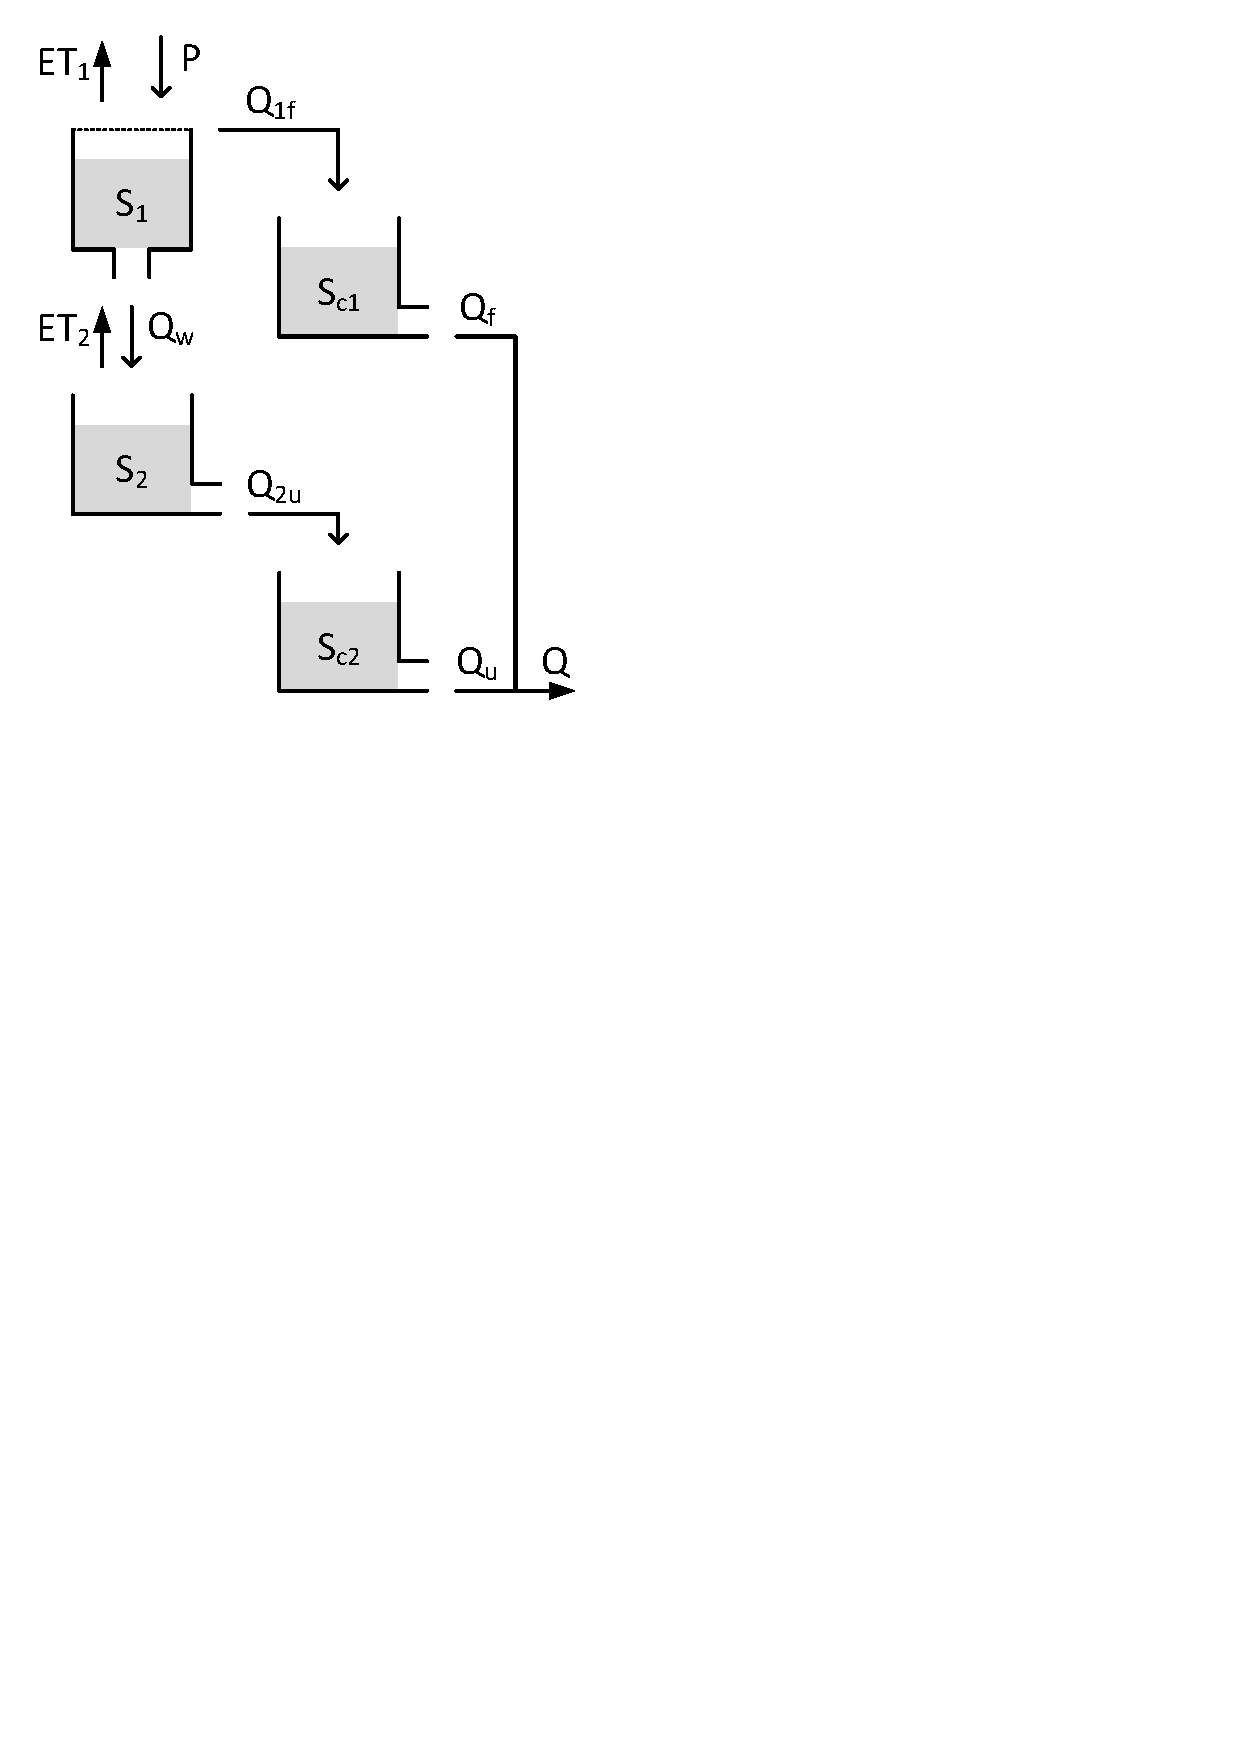
\includegraphics[trim=1cm 18cm 7cm 1cm,width=7cm,keepaspectratio]{./AppA_files/24_schematic.pdf}
\caption{Structure of the MOPEX-1 model} \label{fig:24_schematic}
\end{wrapfigure}

\begin{align}
	\frac{dS_1}{dt} &= P-ET_1-Q_{1f}-Q_w \\
	ET_1 &= \frac{S_1}{S_{b1}}*Ep\\
	Q_{1f} &= \begin{cases}
		P, &\text{if } S_1 \geq S_{b1} \\
		0, & \text{otherwise} \\
	\end{cases} \\
	Q_w &= t_w*S_1
\end{align}

Where $S_1$ [mm] is the current storage in soil moisture and $P$ precipitation $[mm/d]$. Evaporation $ET_1$ $[mm/d]$ depends linearly on current soil moisture, maximum soil moisture $S_{b1}$ [mm] and potential evapotransporation $E_p$ [mm/d]. Saturation excess flow $Q_{1f}$  $[mm/d]$ occurs when the soil moisture bucket exceeds its maximum capacity. Infiltration to deeper groundwater $Q_w$  $[mm/d]$ depends on current soil moisture and time parameter $t_w$  $[d^{-1}]$.

} % end of wrapfigure fix

\begin{align}
	\frac{dS_2}{dt} &= Q_w-ET_2-Q_{2u}\\
	ET_2 &= \frac{S_2}{S_{e}}*Ep\\
	Q_{2u} &= t_u*S_2
\end{align}

Where $S_2$ [mm] is the current groundwater storage, refilled by infiltration from $S_1$. Evaporation $ET_2$ $[mm/d]$ depends linearly on current groundwater and groundwater storage capacity $S_e$ [mm]. Leakage to the slow runoff store $Q_{2u}$ $[mm/d]$ depends on current groundwater level and time parameter $t_u$ $[d^{-1}]$. 

\begin{align}
	\frac{dS_{c1}}{dt} &= Q_{1f}-Q_{f}\\
	Q_f &= t_c*S_{c1}
\end{align}

Where $S_{c1}$ [mm] is current storage in the fast flow routing reservoir, refilled by $Q_{1f}$. Routed flow $Q_f$ depends on the mean residence time parameter $t_c$ $[d^{-1}]$.

\begin{align}
	\frac{dS_{c2}}{dt} &= Q_{2u}-Q_{u}\\
	Q_u &= t_c*S_{c2}
\end{align}

Where $S_{c2}$ [mm] is current storage in the slow flow routing reservoir, refilled by $Q_{2u}$. Routed flow $Q_u$ depends on the mean residence time parameter $t_c$ $[d^{-1}]$. Total simulated flow $Q_t$ $[mm/d]$:

\begin{align}
	Q_t &= Q_f + Q_u
\end{align}

\subsection{Parameter overview}
% Table generated by Excel2LaTeX from sheet 'Sheet1'
\begin{table}[htbp]
  \centering
    \begin{tabular}{lll}
    \toprule
    Parameter & Unit  & Description \\
    \midrule
    $S_{b1}$ & $mm$  & Maximum soil moisture storage \\
    $t_w$ & $d^{-1}$ & Runoff coefficient \\
    $t_u$ & $d^{-1}$ & Runoff coefficient \\
    $S_e$ & $mm$  & Maximum groundwater storage capacity \\
    $t_c$ & $d^{-1}$ & Runoff coefficient \\
    \bottomrule
    \end{tabular}%
  \label{tab:addlabel}%
\end{table}%


\section{Thames Catchment Model (model ID: 25)}
The Thames Catchment Model (TCM) model (fig.~\ref{fig:25_schematic}) is originally intended to be used in zones with similar surface characteristics, rather than catchments as a whole \citep{Moore2001}. It has 4 stores and 6 parameters ($\phi$, $rc$, $\gamma$, $k_1$, $c_a$ and $k_2$). The model aims to represent:

\begin{itemizecompact}
\item Effective rainfall before infiltration;
\item Preferential recharge;
\item Catchment drying through prolonged soil moisture depletion;
\item Groundwater abstraction;
\item Non-linear groundwater flow.
\end{itemizecompact}

\subsection{MARRMoT model name}
m\_25\_tcm\_6p\_4s \\

% Equations
\subsection{Model equations}

% Model layout figure
{ 																	% This ensures it doesn't warp text further down
\begin{wrapfigure}{l}{5cm}
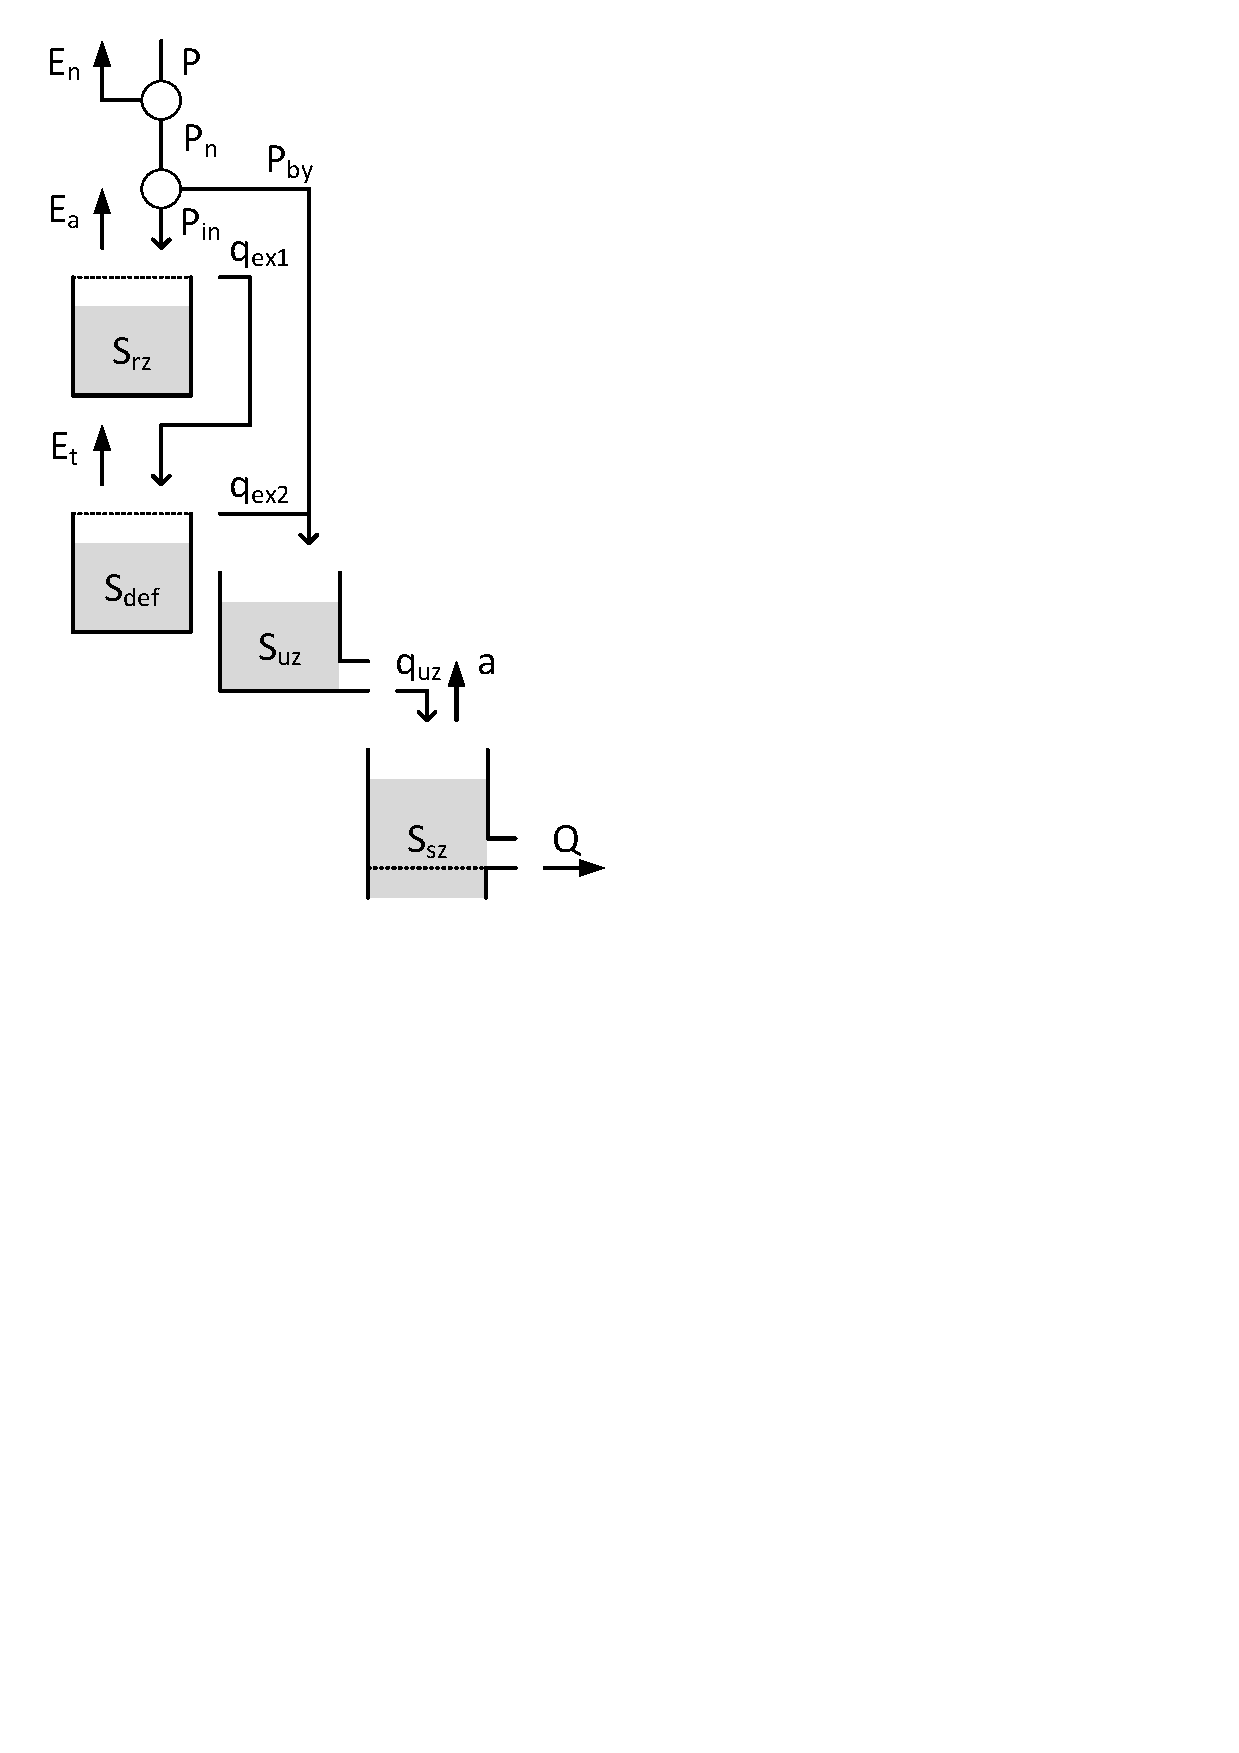
\includegraphics[trim=1cm 14.5cm 7cm 1cm,width=7cm,keepaspectratio]{./AppA_files/25_schematic.pdf}
\caption{Structure of the TCM model} \label{fig:25_schematic}
\end{wrapfigure}

\begin{align}
	\frac{dS_{Rz}}{dt} &= P_{in}-E_a-q_{ex1} \\
	P_{in} &= (1-\phi)*P_n \\
	P_n &= max(P-E_p,0)\\
	E_a &= 
	\begin{cases}
		E_p, & \text{if } S_{rz} > 0 \\
		0, & \text{otherwise}
	\end{cases}\\
	q_{ex1} &= \begin{cases}
		P_{in}, &\text{if } S_{rz} > rc \\
		0, & \text{otherwise} \\
	\end{cases} 
\end{align}

Where $S_{rz}$ [mm] is the current storage in the root zone, refilled by infiltrated precipitation $P_{in}$ $[mm/d]$, and drained by evaporation $E_a$ $[mm/d]$ and storage excess flow $q_{ex1}$ $[mm/d]$. 
$P_{in}$ is the fraction $(1-\phi)$ [-] of net precipitation $P_n$ $[mm/d]$ that is not preferential recharge. 
$P_n$ is the difference between precipitation $P$ [mm/d] and potential evapotranspiration $E_p$ [mm/d] per time step. 
$E_a$ occurs at the net potential rate whenever possible.
$q_{ex1}$ occurs only when the store is at maximum capacity $rc$ [mm].

} % end of wrapfigure fix

\begin{align}
	\frac{dS_{def}}{dt} &= E_t + q_{ex2} - q_{ex1}\\
	E_t &=\begin{cases}
		\gamma*E_p, &\text{if } S_{rz} = 0 \\
		0, & \text{otherwise} \\
	\end{cases} \\
	 q_{ex2}  &= \begin{cases}
		q_{ex1}, &\text{if } S_{def} = 0 \\
		0, & \text{otherwise} \\
	\end{cases}
\end{align}

Where $S_{def}$ [mm] is the current storage in the soil moisture \emph{deficit} store.
The deficit is increased by evaporation $E_t$ $[mm/d]$ and percolation $q_{ex2}$ $[mm/d]$.
The deficit is decreased by overflow from the upper store $q_{ex1}$.
$E_t$ only occurs when the upper zone is empty and at a fraction $\gamma$ [-] of $E_p$.
$q_{ex2}$ only occurs when the deficit is zero.

\begin{align}
	\frac{dS_{uz}}{dt} &= P_{by} + q_{ex2} - q_{uz} \\
	P_{by} &= \phi*P_n\\
	q_{uz} &= k_1*S_{uz}
\end{align}
  
Where $S_{uz}$ is the current storage in the unsaturated zone, refilled by preferential recharge $P_{by}$ $[mm/d]$ and percolation $q_{ex2}$ $[mm/d]$, and drained by groundwater flow $q_{uz}$ $[mm/d]$.
$P_{by}$ is a fraction $\phi$ [-] of $P_n$.
$q_{uz}$ has a linear relation with storage through time parameter $k_1$ $[d^{-1}]$.

\begin{align}
	\frac{dS_{sz}}{dt} &= q_{uz} -a-Q\\
	a &= c_a\\
	Q &= \begin{cases}
		k_2*S_{sz}^2, &\text{if } S_{sz} > 0 \\
		0, & \text{otherwise} \\
	\end{cases}
\end{align}

Where $S_{sz}$ [mm] is the current storage in the saturated zone, refilled by groundwater flow $q_{uz}$ $[mm/d]$ and drained by abstractions $a$ $[mm/d]$ and outflow $Q$ $[mm/d]$.
$a$ occurs at a constant rate $c_a$ $[mm/d]$.
Abstractions can draw down the aquifer below the runoff generating threshold. 
$Q$ has a quadratic relation with storage through parameter $k_2$ $[mm^{-1} d^{-1}]$.

\newpage
\subsection{Parameter overview}
% Table generated by Excel2LaTeX from sheet 'Sheet1'
\begin{table}[htbp]
  \centering
    \begin{tabular}{lll}
    \toprule
    Parameter & Unit  & Description \\
    \midrule
    $\phi$ & $-$   & Fraction of net precipitation that is preferntial flow \\
    $rc$  & $mm$  & Maximum root zone storage \\
    $\gamma$ & $-$   & Transpiration reduction factor \\
    $k_1$ & $d^{-1}$ & Runoff coefficient \\
    $c_a$ & $mm~d^{-1}$ & Abstraction rate \\
    $k_2$ & $d^{-1}$ & Runoff coefficient \\
    \bottomrule
    \end{tabular}%
  \label{tab:addlabel}%
\end{table}%


\section{Flex-I (model ID: 26)}
The Flex-I model (fig.~\ref{fig:26_schematic}) is the part of a model development exercise \citep{Fenicia2008}. It has 4 stores and 10 parameters ($I_{max}$, $UR_{max}$, $\beta$, $D$, $Perc_{max}$, $L_p$, $N_{lag,f}$, $N_{lag,s}$, $K_f$ and $K_s$). The model aims to represent:

\begin{itemizecompact}
\item Interception by vegetation;
\item Infiltration and saturation excess flow based on a distribution of different soil depths;
\item A split between fast saturation excess flow and preferential recharge to a slow store;
\item Percolation from the unsaturated zone to a slow runoff store.
\end{itemizecompact}

\subsection{MARRMoT model name}
m\_26\_flexi\_10p\_4s \\

% Equations
\subsection{Model equations}

% Model layout figure
{ 																	% This ensures it doesn't warp text further down
\begin{wrapfigure}{l}{7cm}
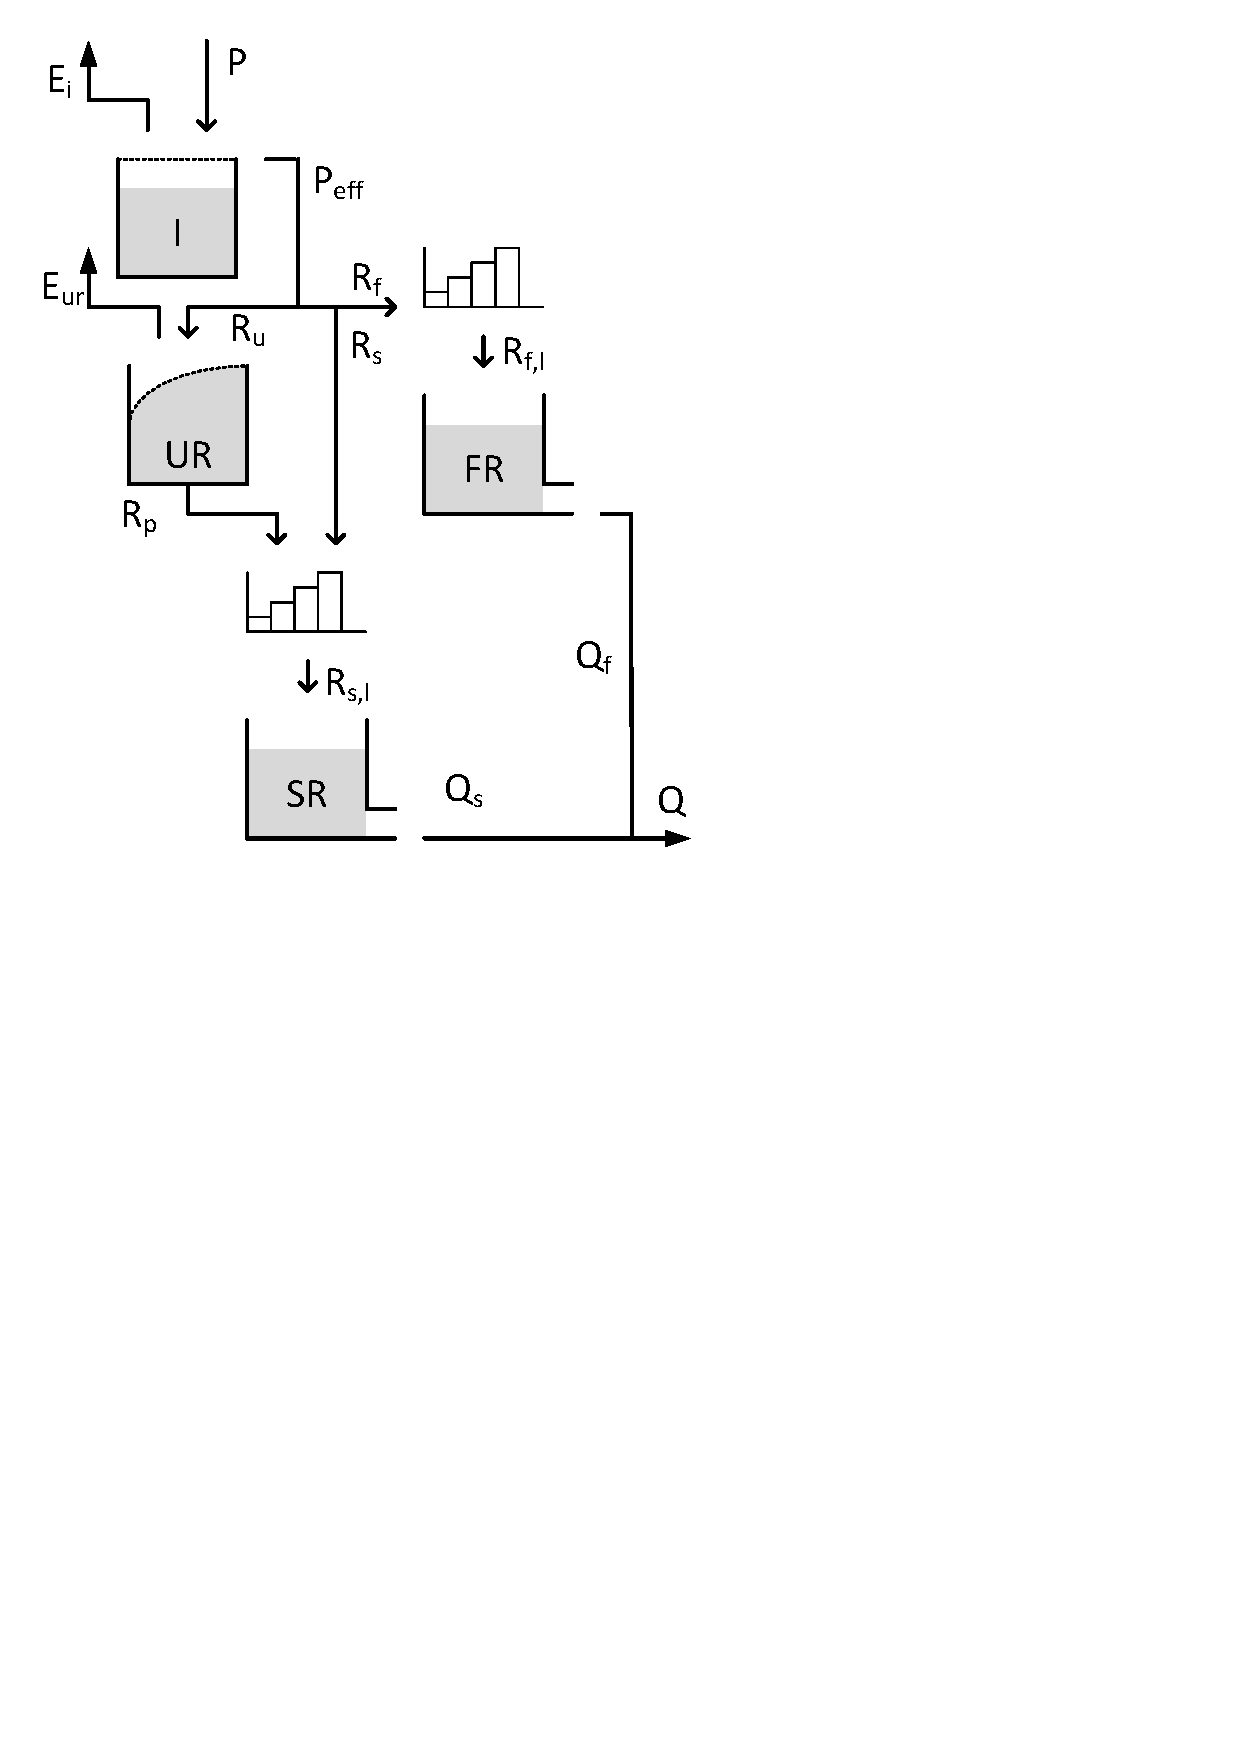
\includegraphics[trim=1cm 15cm 7cm 1cm,width=7cm,keepaspectratio]{./AppA_files/26_schematic.pdf}
\caption{Structure of the Flex-I model} \label{fig:26_schematic}
\end{wrapfigure}

\begin{align}
	\frac{dI}{dt} &= P-E_i-P_{eff} \\
	E_i &= \begin{cases}
		Ep &\text{, if } I > 0\\
		0 &\text{, otherwise }\\
	\end{cases}\\
	P_eff &= \begin{cases}
		P &\text{, if } I \geq I_{max}\\
		0 &\text{, otherwise }\\
	\end{cases}	
\end{align}

Where I is the current interception storage [mm], P $[mm/d]$ incoming precipitation, $E_i$ $[mm/d]$ evaporation from the interception store and $P_{eff}$  $[mm/d]$ interception excess routed to soil moisture. Evaporation occurs at the potential rate $E_p$ [mm/d] whenever possible. Interception excess occurs when the interception store exceeds its maximum capacity $I_{max}$ [mm].

} % end of wrapfigure fix
\vspace{1cm}

\begin{align}
	\frac{dUR}{dt} &= R_u - E_{ur} - R_p \\
	R_U &= (1 - C_r) * P_{eff}\\
	C_r &= \Big[1+exp\Big(\frac{-UR/UR_{max} + 1/2}{\beta}\Big)\Big]^{-1}\\
	%R_u &= (1 - \Big[1+exp\Big(\frac{-UR/UR_{max} + 1/2}{\beta}\Big)\Big]^{-1}) * P_{eff}\\
	E_{ur} &= E_p * min\Big(1, \frac{UR}{UR_{max}} \frac{1}{L_p}\Big)\\
	P_s&= Perc_{max} * \frac{-UR}{UR_{max}}
\end{align}
  
Where UR is the current storage in the unsaturated zone [mm]. $R_u$ $[mm/d]$ is the inflow into UR based on its current storage compared to maximum storage $UR_{max}$ [mm] and a shape distribution parameter $\beta$ [-].  $E_{ur}$ the evaporation $[mm/d]$ from UR which follows a linear relation between current and maximum storage until a threshold $L_p$ [-] is exceeded. $P_s$ is the percolation from UR to the slow reservoir SR $[mm/d]$, based on a maximum percolation rate $Perc_{max}$ [mm], relative to the fraction of current storage and maximum storage. $P_{eff}$ is routed towards the unsaturated zone based on $Cr$, with the remainder being divided into preferential recharge $R_s$ $[mm/d]$ and fast runoff $R_f$ $[mm/d]$:

\begin{align}
	R_s &= (P_{eff} - R_u)*D\\
	R_f &= (P_{eff} - R_u)*(1-D)
\end{align}

Where $R_s$ and $R_f$ are the flows $[mm/d]$ to the slow and fast runoff reservoir respectively, based on runoff partitioning coefficient D [-]. Both are lagged by linearly increasing triangular transformation functions with parameters $N_{lag,s}$ [d] and $N_{lag,f}$ [d] respectively, that give the number of days over which $R_s$ and $R_f$ need to be transformed. Percolation $R_p$ is added to $R_s$ before the transformation to $R_{s,l}$ occurs.

\begin{align}
	\frac{dFR}{dt} &= R_{f,l} - Q_f\\
	Q_f &= K_f * FR 
\end{align}

Where FR is the current storage [mm] in the fast flow reservoir. Outflow $Q_f$ $[mm/d]$ from the reservoir has a linear relation with storage through time scale parameter $K_f$ [$d^{-1}$]. 

\begin{align}
	\frac{dSR}{dt} &= R_{s,l} - Q_s \\
	Q_s &= K_s * SR 
\end{align}

Where SR is the current storage [mm] in the slow flow reservoir. Outflow $Q_s$ $[mm/d]$ from the reservoir has a linear relation with storage through time scale parameter $K_s$ [$d^{-1}$]. Total outflow Q  $[mm/d]$:

\begin{equation}
	Q = Q_f + Q_s
\end{equation}

\subsection{Parameter overview}
% Table generated by Excel2LaTeX from sheet 'Sheet1'
\begin{table}[htbp]
  \centering
    \begin{tabular}{lll}
    \toprule
    Parameter & Unit  & Description \\
    \midrule
    $I_{max}$ & $mm$  & Maximum interception storage \\
    $UR_{max}$ & $mm$  & Maximum soil moisture storage \\
    $\beta$ & $-$   & Shape parameter \\
    $D$   & $-$   & Fraction effective precipitation to slow store \\
    $Perc_{max}$ & $mm~d^{-1}$ & Maximum percolation rate \\
    $L_p$ & $-$   & Wilting point as fraction of $UR_{max}$ \\
    $N_{lag,f}$ & $d$   & Unit Hydrograph time base \\
    $N_{lag,s}$ & $d$   & Unit Hydrograph time base \\
    $K_f$ & $d^{-1}$ & Runoff coefficient \\
    $K_s$ & $d^{-1}$ & Runoff coefficient \\
    \bottomrule
    \end{tabular}%
  \label{tab:addlabel}%
\end{table}%

\subsection{Tank model (model ID: 27)}
The Tank Model (fig.~\ref{fig:27_schematic}) is originally developed for use constantly saturated soils in Japan \citep{Sugawara1979,Sugawara1995}. It has 4 stores and 12 parameters ($A_0$, $A_1$, $A_2$, $t_1$, $t_2$, $B_0$, $B_1$, $t_3$, $C_0$, $C_1$, $t_4$ and $D_1$). The model aims to represent:

\begin{itemizecompact}
\item Runoff on increasing time scales with depth.
\end{itemizecompact}

\subsubsection{File names}
\begin{tabular}{@{}ll}
Model: &m\_27\_tank\_12p\_4s \\
Parameter ranges: &m\_27\_tank\_12p\_4s\_parameter\_ ranges \\
\end{tabular}

% Equations
\subsubsection{Model equations}

% Model layout figure
{ 																	% This ensures it doesn't warp text further down
\begin{wrapfigure}{l}{4cm}
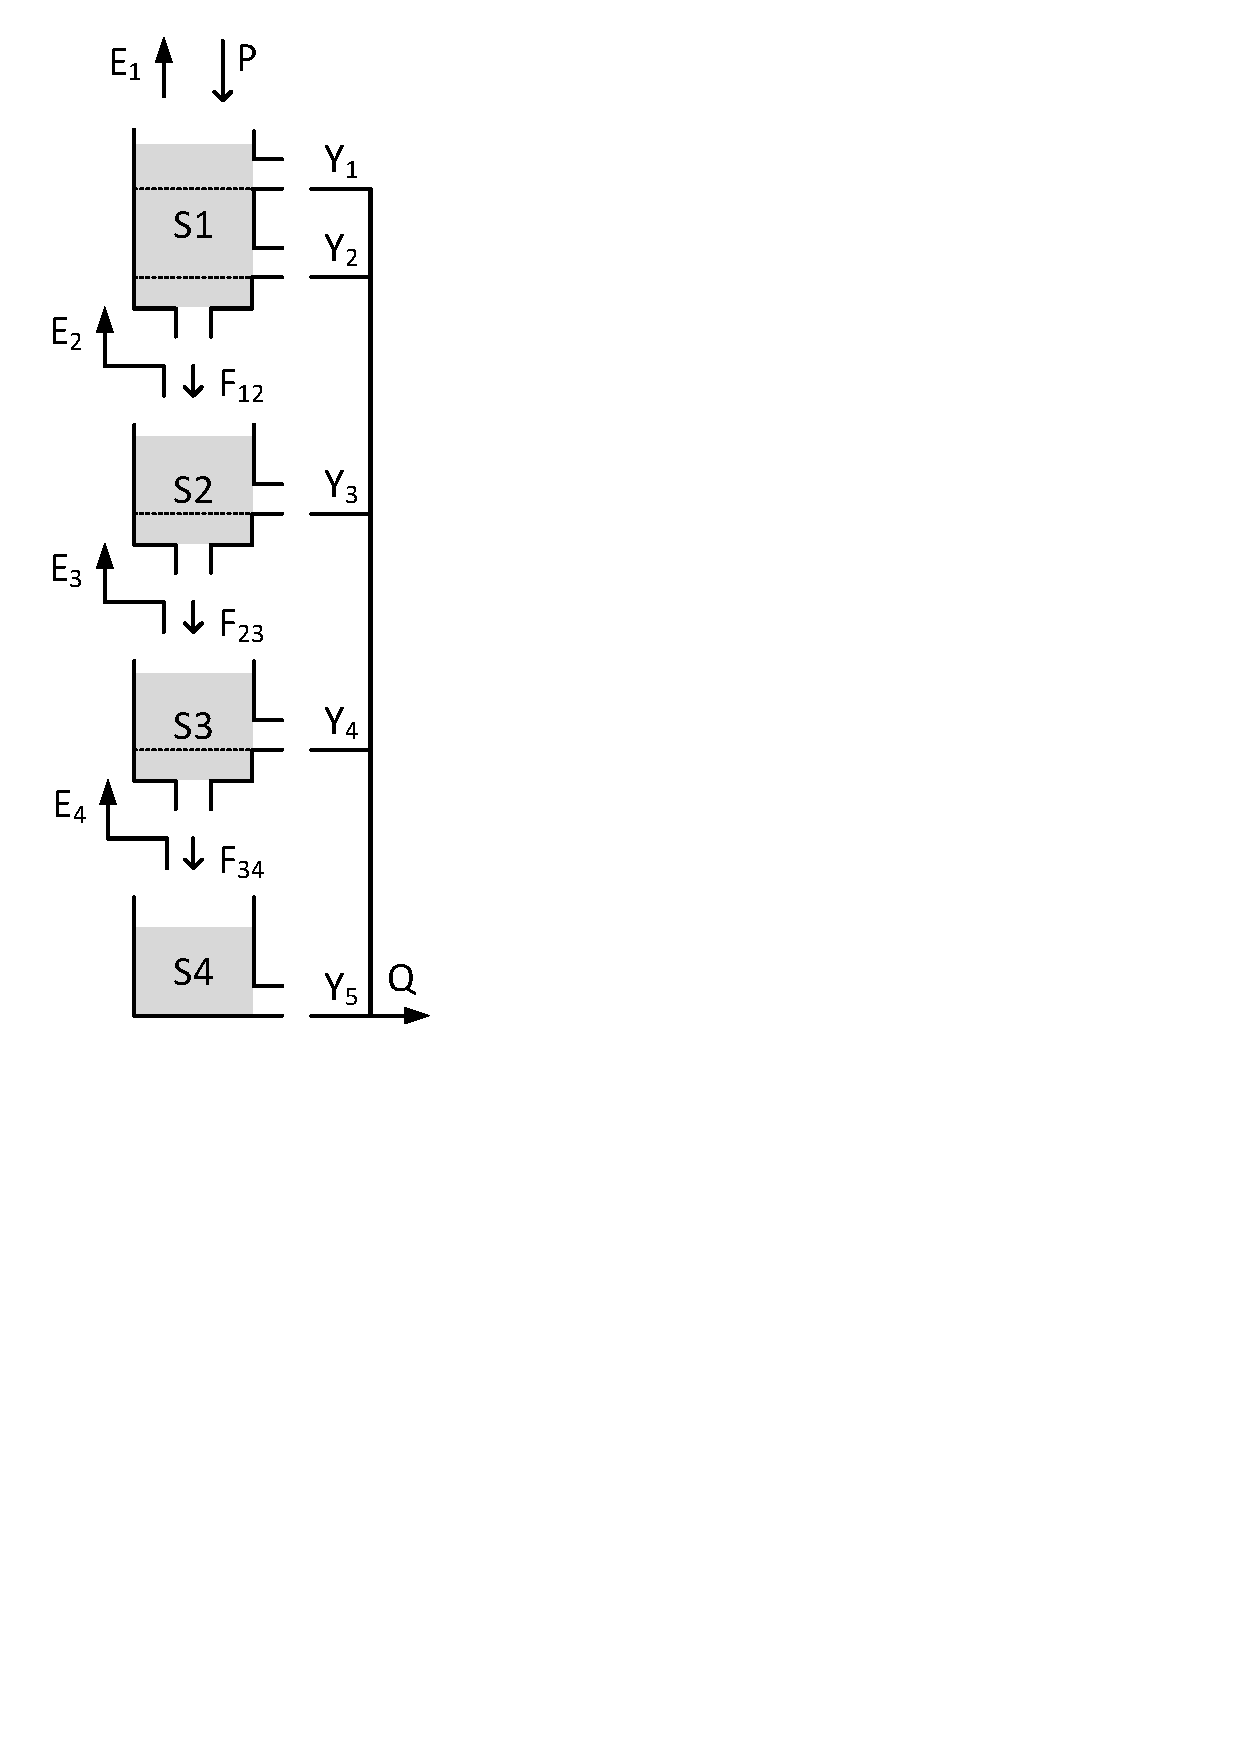
\includegraphics[trim=1cm 12cm 7cm 1cm,width=7cm,keepaspectratio]{./files/27_schematic.pdf}
\caption{Structure of the Tank Model} \label{fig:27_schematic}
\end{wrapfigure}

\begin{align}
	\frac{dS_1}{dt} &= P-E_1-F_{12}-Y_2-Y_1 \\
	E_1 &= \begin{cases}
		Ep, &\text{if } S_1 > 0 \\
		0, & \text{otherwise} \\
	\end{cases} \\
	F_{12} &= A_0*S_1\\
	Y_2 &= 
	\begin{cases}
		A_2*(S_1-t_2), & \text{if } S_1 > t_2 \\
		0, & \text{otherwise}
	\end{cases}\\
	Y_1 &= 
	\begin{cases}
		A_1*(S_1-t_1), & \text{if } S_1 > t_1 \\
		0, & \text{otherwise}\\
	\end{cases}
\end{align}

Where $S_1$ [mm] is the current storage in the upper zone, refilled by precipitation $P$ $[mm/d]$ and drained by evaporation $E_1$ $[mm/d]$, drainage $F_{12}$ $[mm/d]$ and surface runoff $Y_1$ $[mm/d]$ and $Y_2$ $[mm/d]$. $E_1$ occurs at the potential rate $E_p$ $[mm/d]$ if water is available. Drainage to the intermediate layer has a linear relationship with storage through time scale parameter $A_0$ $[d^{-1}]$. Surface runoff $Y_2$ and $Y_1$ occur when $S_1$ is above thresholds $t_2$ [mm] and $t_1$ [mm] respectively. Both are linear relationships through time parameters $A_2$ $[d^{-1}]$ and $A_1$ $[d^{-1}]$ respectively.

} % end of wrap figure

\begin{align}
	\frac{dS_2}{dt} &= F_{12}-E_2-F_{23}-Y_3\\
	E_2 &= \begin{cases}
		Ep, &\text{if } S_1 = 0 ~\&~ S_2 > 0\\
		0, & \text{otherwise} \\
	\end{cases} \\
	F_{23} &= B_0*S_2\\
	Y_3 &= 
	\begin{cases}
		B_1*(S_2-t_3), & \text{if } S_2 > t_3 \\
		0, & \text{otherwise}
	\end{cases}
\end{align}

Where $S_2$ [mm] is the current storage in the intermediate zone, refilled by drainage $F_{12}$ from the upper zone and drained by evaporation $E_2$ $[mm/d]$, drainage $F_{23}$ $[mm/d]$ and intermediate discharge $Y_3$ $[mm/d]$. $E_2$ occurs at the potential rate $E_p$ if water is available and the upper zone is empty. Drainage to the third layer $F_{23}$ has a linear relationship with storage through time scale parameter $B_0$ $[d^{-1}]$. Intermediate runoff $Y_3$ occurs when $S_2$ is above threshold $t_3$ [mm] and has a linear relationship with storage through time scale parameter $B_1$ $[d^{-1}]$.

\begin{align}
	\frac{dS_3}{dt} &= F_{23}-E_3-F_{34}-Y_4\\
	E_3 &= \begin{cases}
		Ep, &\text{if } S_1 = 0 ~\&~ S_2 = 0 ~\&~ S_3 > 0\\
		0, & \text{otherwise} \\
	\end{cases} \\
	F_{34} &= C_0*S_3\\
	Y_4 &= 
	\begin{cases}
		C_1*(S_3-t_4), & \text{if } S_3 > t_4 \\
		0, & \text{otherwise}
	\end{cases}
\end{align}

Where $S_3$ [mm] is the current storage in the sub-base zone, refilled by drainage $F_{23}$ from the intermediate zone and drained by evaporation $E_3$ $[mm/d]$, drainage $F_{34}$ $[mm/d]$ and sub-base discharge $Y_4$ $[mm/d]$. $E_3$ occurs at the potential rate $E_p$ if water is available and the upper zones are empty. Drainage to the fourth layer $F_{34}$ has a linear relationship with storage through time scale parameter $C_0$ $[d^{-1}]$. Sub-base runoff $Y_4$ occurs when $S_3$ is above threshold $t_4$ [mm] and has a linear relationship with storage through time scale parameter $C_1$ $[d^{-1}]$.

\begin{align}
	\frac{dS_4}{dt} &= F_{34}-E_4-Y_5\\
	E_4 &= \begin{cases}
		Ep, &\text{if } S_1 = 0 ~\&~ S_2 = 0 ~\&~ S_3 = 0 ~\&~ S_4 > 0\\
		0, & \text{otherwise} \\
	\end{cases} \\
	Y_5 &= D_1*S_4
\end{align}

Where $S_4$ [mm] is the current storage in the base layer, refilled by drainage $F_{34}$ from the sub-base zone and drained by evaporation $E_4$ $[mm/d]$ and baseflow $Y_5$ $[mm/d]$. $E_4$ occurs at the potential rate $E_p$ if water is available and the upper zones are empty. Baseflow $Y_5$ has a linear relationship with storage through time scale parameter $D_1$ $[d^{-1}]$. Total runoff:

\begin{align}
	Q_t &= Y_1+Y_2+Y_3+Y_4+Y_5
\end{align}

\subsubsection{Parameter overview}
% Table generated by Excel2LaTeX from sheet 'Sheet1'
\begin{table}[htbp]
  \centering
    \begin{tabular}{lll}
    \toprule
    Parameter & Unit  & Description \\
    \midrule
    $A_0$ & $d^{-1}$ & Runoff coefficient \\
    $A_1$ & $d^{-1}$ & Runoff coefficient \\
    $A_2$ & $d^{-1}$ & Runoff coefficient \\
    $t_1$ & $mm$  & Threshold for runoff generation \\
    $t_2$ & $mm$  & Threshold for runoff generation \\
    $B_0$ & $d^{-1}$ & Runoff coefficient \\
    $B_1$ & $d^{-1}$ & Runoff coefficient \\
    $t_3$ & $mm$  & Threshold for runoff generation \\
    $C_0$ & $d^{-1}$ & Runoff coefficient \\
    $C_1$ & $d^{-1}$ & Runoff coefficient \\
    $t_4$ & $mm$  & Threshold for runoff generation \\
    $D_1$ & $d^{-1}$ & Runoff coefficient \\
    \bottomrule
    \end{tabular}%
  \label{tab:addlabel}%
\end{table}%


\subsection{Xinanjiang model (model ID: 28)}
The Xinanjiang model (fig.~\ref{fig:28_schematic}) is originally intended for use in humid or semi-humid regions in China \citep{Zhao1992}. The model uses a variable contributing area to simulate runoff. The version presented here uses a double parabolic curve to simulate tension water capacities within the catchment \citep{Jayawardena2000}, instead of the original single parabolic curve. The model has 4 stores and 12 parameters ($A_{im}$, $a$, $b$, $W_{max}$, $LM$, $c$, $S_{max}$, $Ex$, $k_I$, $k_G$, $c_I$ and $c_G$). The model aims to represent:

\begin{itemizecompact}
\item Runoff from impervious areas;
\item Variable distribution of tension water storage capacities in the catchment;
\item Variable contributing area of free water storages;
\item Direct surface runoff from the contributing free area;
\item Delayed interflow and baseflow from the contributing free area.
\end{itemizecompact}

\subsubsection{File names}
\begin{tabular}{@{}ll}
Model: &m\_28\_xinanjiang\_12p\_4s \\
Parameter ranges: &m\_28\_xinanjiang\_12p\_4s\_parameter\_ ranges \\
\end{tabular}

% Equations
\subsubsection{Model equations}

% Model layout figure
{ 																	% This ensures it doesn't warp text further down
\begin{wrapfigure}{l}{6cm}
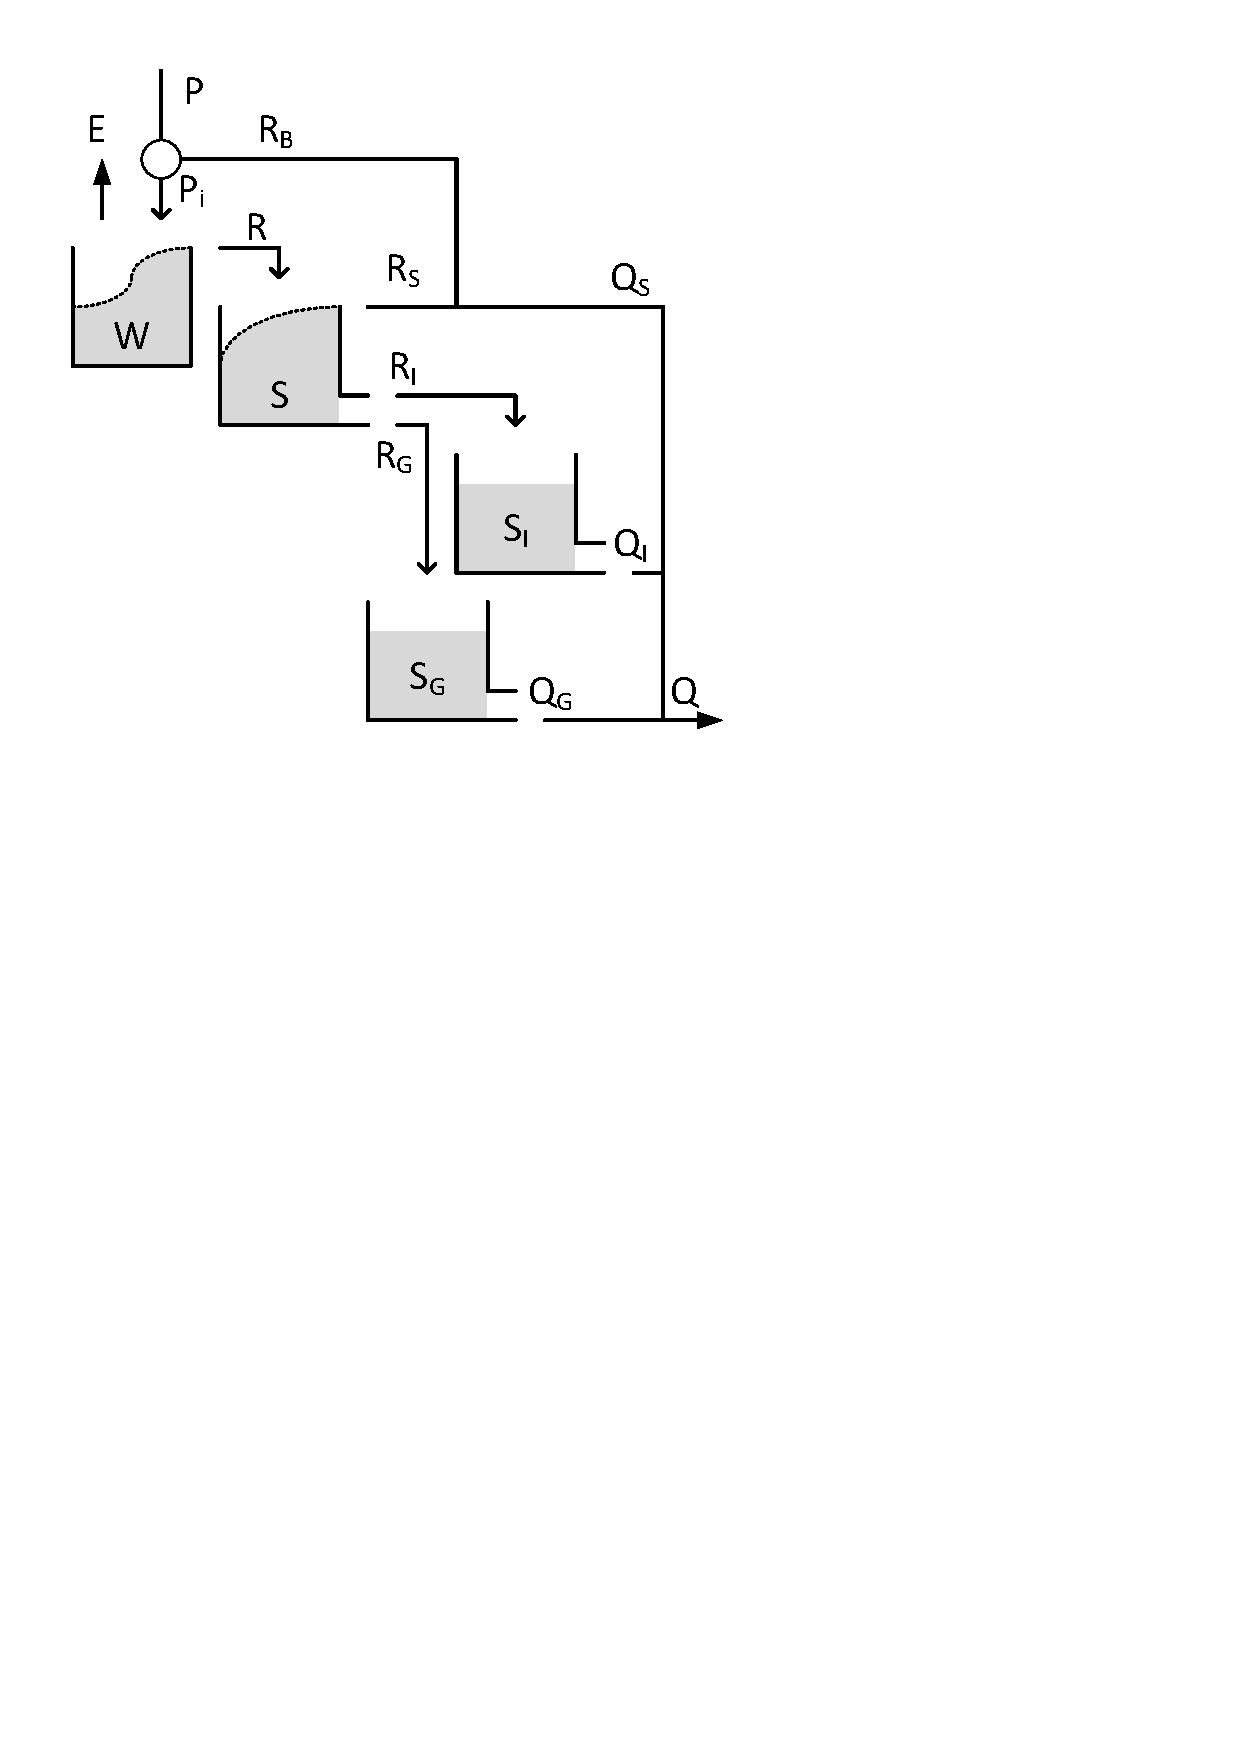
\includegraphics[trim=1cm 17cm 7cm 1cm,width=7cm,keepaspectratio]{./files/28_schematic.pdf}
\caption{Structure of the Xinanjiang model} \label{fig:28_schematic}
\end{wrapfigure}

\begin{align}
	\frac{dW}{dt} &= P_i-E-R \\
	P_i &= (1-A_{im})*P \\
	R &= 
	\begin{cases}
		P_i * \left[(0.5-a)^{1-b}\left(\frac{W}{W_{max}}\right)^b\right] , & \text{if } \frac{W}{W_{max}} \leq 0.5-a \\
		P_i * \left[1-(0.5+a)^{1-b}\left(1-\frac{W}{W_{max}}\right)^b\right] , & \text{otherwise}
	\end{cases} \\
	E &= \begin{cases}
		E_p , & \text{if } W > LM \\
		\frac{W}{LM}E_p , & \text{if } c*LM \geq W \leq LM \\
		c*E_p , & \text{otherwise}
	\end{cases}
\end{align}

} % end of wrapfigure fix
\vspace{2cm}
Where $W$ [mm] is the current tension water storage, refilled by a infiltration $P_i$ $[mm/d]$ and drained by evaporation $E$ $[mm/d]$ and runoff $R$ $[mm/d]$.
$P_i$ is the fraction of precipitation $P$ $[mm/d]$ that does not fall on impervious area $A_{im}$ [-].
Runoff generation $R$ uses a double parabolic curve to determine the fraction of catchment area that is at full tension storage and thus can contribute to runoff generation. 
This curve relies on shape parameters $a$ [-] and $b$ [-], and maximum tension water storage $W_{max}$ [mm].
Evaporation rate $E$ declines as tension water storage decreases.
Evaporation occurs at the potential rate $E_p$ $[mm/d]$ if storage $W$ is above threshold $LM$ [mm], and reduces linearly below that up to a second threshold $c*LM$ [-]*[mm].
Below this threshold evaporation occurs at a constant rate $c*E_p$.

\begin{align}
	\frac{dS}{dt} &= R-R_S-R_I-R_G\\
	R_S &= R*\left(1-\left(1-\frac{S}{S_{max}}\right)^{Ex}\right) \\
	R_I  &= k_I * S * \left(1-\left(1-\frac{S}{S_{max}}\right)^{Ex}\right)\\
	R_G  &= k_G * S * \left(1-\left(1-\frac{S}{S_{max}}\right)^{Ex}\right)
\end{align}

Where $S$ [mm] is the current storage of free water, refilled by runoff $R$ from filled tension water areas, and drained by surface runoff $R_S$ [mm/d], interflow $R_I$ [mm/d] and baseflow $R_G$ [mm/d].
All runoff components rely on a parabolic equation to simulate variable contributing areas of the catchment, dependent on maximum free water storage $S_{max}$ [mm] and shape parameter $Ex$ [-]. 
$R_I$ also uses a time coeficient $k_I$ $[d^{-1}]$.
$R_G$ uses a time coeficient $k_G$ $[d^{-1}]$.

\begin{align}
	\frac{dS_I}{dt} &= R_{I} - Q_I\\
	Q_I &= c_I*S_I 
\end{align}

Where $S_I$ [mm] is the current storage in the interflow routing reservoir, filled by interflow from free water $R_I$ and drained by delayed interflow $Q_I$ $[mm/d]$.
$Q_I$ uses a time coefficient $c_I$ $[d^{-1}]$.

\begin{align}
	\frac{dS_G}{dt} &= R_{G} - Q_G\\
	Q_G &= c_G*S_G
\end{align}

Where $S_G$ [mm] is the current storage in the baseflow routing reservoir, filled by baseflow from free water $R_G$ and drained by delayed baseflow $Q_G$ $[mm/d]$.
$Q_G$ uses a time coefficient $c_G$ $[d^{-1}]$.
Total flow depends on four separate runoff components:

\begin{align}
	Q_t &= Q_S + Q_I + Q_G \\
	Q_S &= R_S + R_B \\
	R_B &= A_{im}*P
\end{align}

Where $R_B$ [mm/d] is direct rainoff generated by precipitation $P$ [mm/d] on the fraction impervious area $A_{im}$ [-].

\subsubsection{Parameter overview}
% Table generated by Excel2LaTeX from sheet 'Sheet1'
\begin{table}[htbp]
  \centering
    \begin{tabular}{lll}
    \toprule
    Parameter & Unit  & Description \\
    \midrule
    $A_{im}$ & $-$   & Fraction impervious area \\
    $a$   & $-$   & Contributing area curve inflection point \\
    $b$   & $-$   & Contributing area curve shape parameter \\
    $W_{max}$ & $mm$  & Maximum tension water storage \\
    $LM$  & $mm$  & Threshold for evaporation behaviour change \\
    $c$   & $-$   & Threshold and evaporation reduction factor \\
    $S_{max}$ & $mm$  & Maximum free water storage \\
    $Ex$  & $-$   & Contributing area curve shape parameter \\
    $k_I$ & $d^{-1}$ & Runoff coefficient \\
    $k_G$ & $d^{-1}$ & Runoff coefficient \\
    $c_I$ & $d^{-1}$ & Runoff coefficient \\
    $c_G$ & $d^{-1}$ & Runoff coefficient \\
    \bottomrule
    \end{tabular}%
  \label{tab:addlabel}%
\end{table}%

\subsection{HyMOD (model ID: 29)}
The HyMOD model (fig.~\ref{fig:29_schematic}) combines a PDM-like soil moisture routine (e.g. \citet{Moore2007}) with a Nash cascade of three linear reservoirs that simulates fast flow and a single linear reservoir intended to simulate slow flow \citep{Wagener2001,Boyle2001}. Although the model was originally intended as a flexible structure where the user defines which processes to include, this study includes only a single version that is commonly used. It has 5 parameters ($S_{max}$, $b$, $a$, $k_f$ and $k_s$) and 5 stores. The model aims to represent:

\begin{itemizecompact}
\item Different soil depths throughout the catchment;
\item Separation of flow into fast and slow flow.
\end{itemizecompact}

\subsubsection{File names}
\begin{tabular}{@{}ll}
Model: &m\_29\_hymod\_5p\_5s \\
Parameter ranges: &m\_29\_hymod\_5p\_5s\_parameter\_ ranges \\
\end{tabular}

% Equations
\subsubsection{Model equations}

% Model layout figure
{ 																	% This ensures it doesn't warp text further down
\begin{wrapfigure}{l}{7cm}
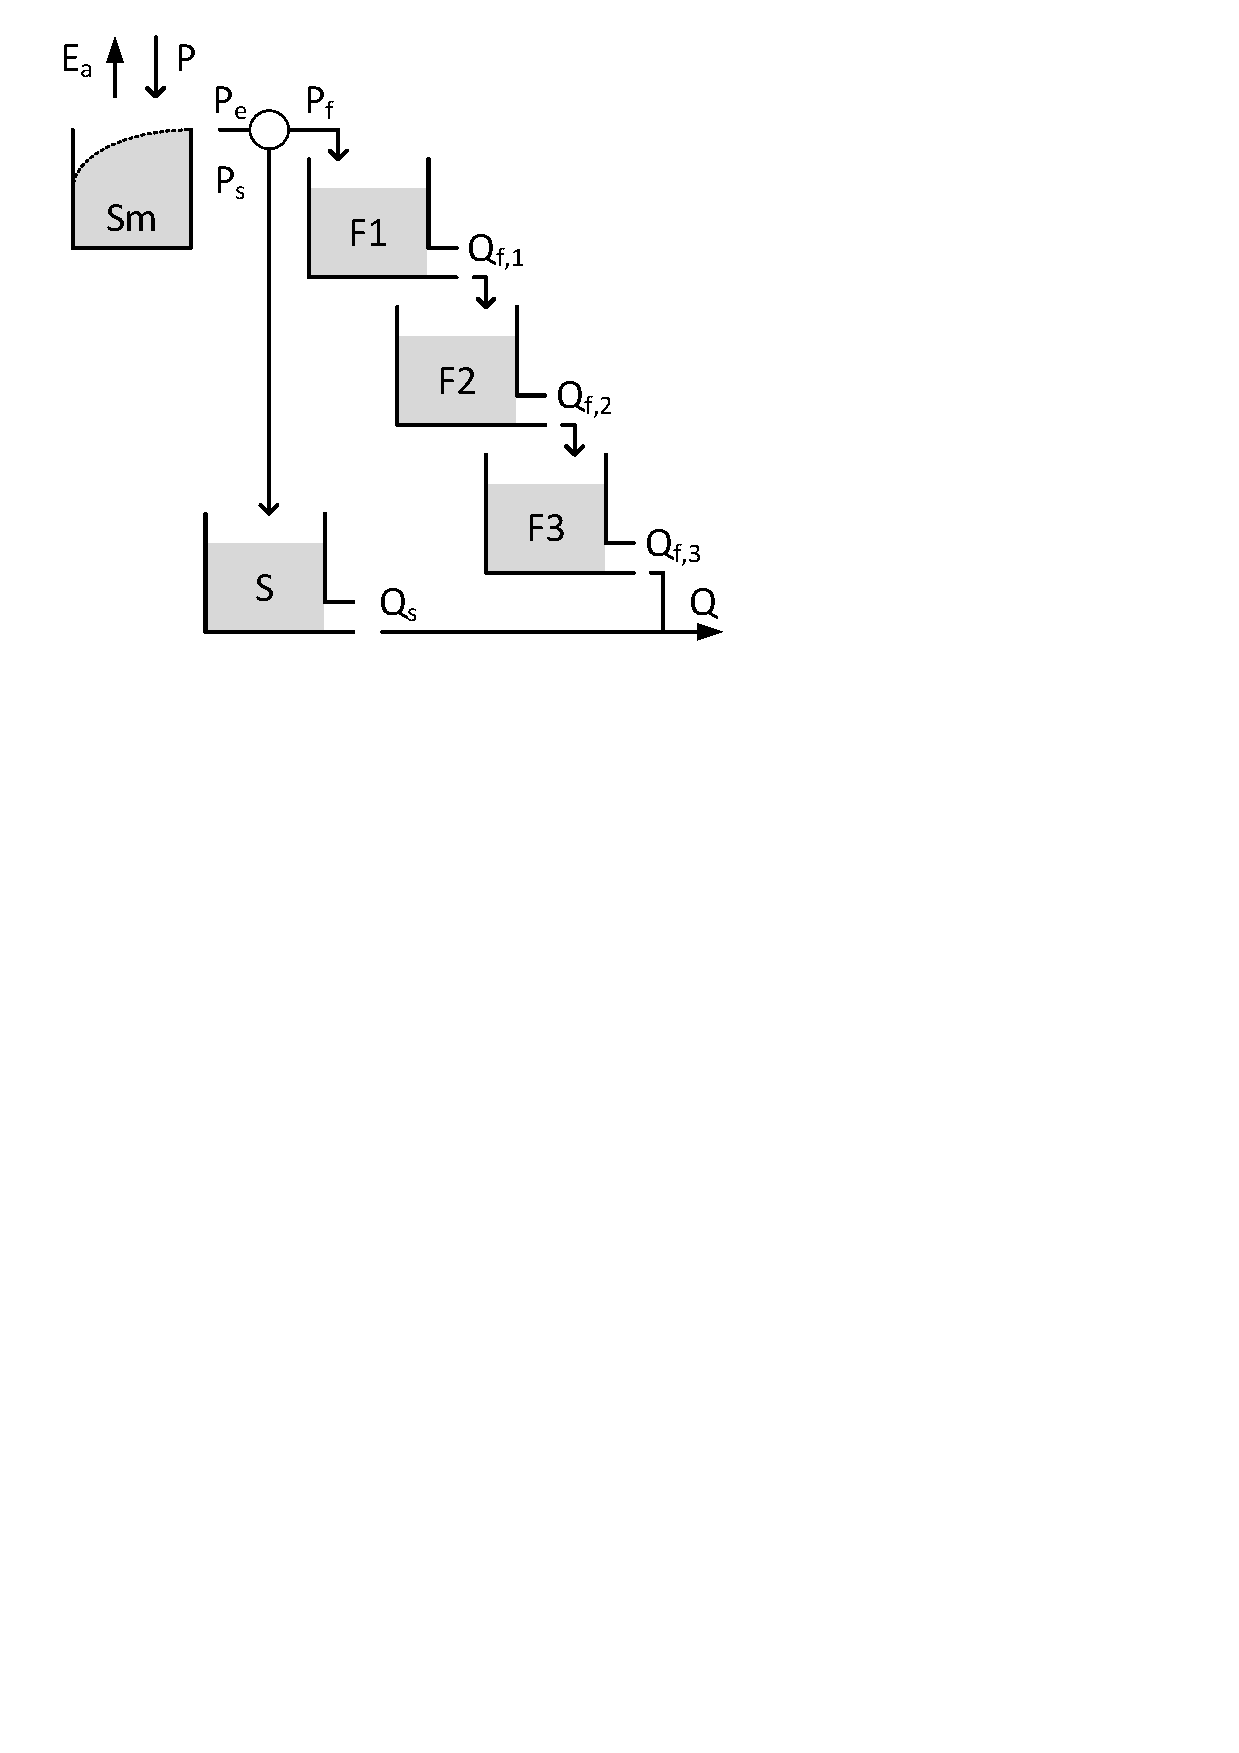
\includegraphics[trim=1cm 18.5cm 7cm 1cm,width=7cm,keepaspectratio]{./files/29_schematic.pdf}
\caption{Structure of the HyMOD model} \label{fig:29_schematic}
\end{wrapfigure}

\begin{align}
	\frac{dSm}{dt} &= P-E_a-P_e \\
	E_a &= \frac{Sm}{S_{max}}*E_p\\
	P_e &= \left(1-\left(1-\frac{S}{S_{max}}\right)^b\right)*P
\end{align}

Where Sm is the current storage in Sm [mm], $S_{max}$ [mm] is the maximum storage in Sm, $E_a$ and $E_p$ the actual and potential evapotranspiration respectively [mm/d] and b is the soil depth distribution parameter [-]. P [mm/d] is the precipitation input.

\begin{align}
	\frac{dF_1}{dt} &= P_f - Q_{f,1}\\
	P_f &= a*P_e \\
	Q_{f,1} &= k_f*S_{f,1} 
\end{align}

} % end of wrapfigure fix

\noindent Where $F_1$ is the current storage in store $F_1$ [mm], $a$ the fraction of $P_e$ that flows into the fast stores and $k_f$ the runoff coefficient of the fast stores. Stores $F_2$ and $F_3$ take the outflow of the previous store as input ($Q_{f,1}$ and $Q_{f,2}$ respectively) and generate outflow analogous to the equations above.

\begin{align}
	\frac{dS}{dt} &= P_s - Q_s\\
	P_s &= (1-a)*P_e \\
	Q_s &= k_s*S 
\end{align}
  
\noindent Where $S$ is the current storage in store S [mm], $1-a$ [-] the fraction of $P_e$ that flows into the slow store and $k_s$ the runoff coefficient of the slow store. Total outflow:

\begin{align}
	Q_t &= Q_s + Q_{f,3}
\end{align}

\subsubsection{Parameter overview}
% Table generated by Excel2LaTeX from sheet 'Sheet1'
\begin{table}[htbp]
  \centering
    \begin{tabular}{lll}
    \toprule
    Parameter & Unit  & Description \\
    \midrule
    $S_{max}$ & $mm$  & Maximum soil moisture storage \\
    $b$   & $-$   & Contributing area curve shape parameter \\
    $a$   & $-$   & Fraction of effective precipitation that is fast flow \\
    $k_f$ & $d^{-1}$ & Runoff coefficient \\
    $k_s$ & $d^{-1}$ & Runoff coefficient \\
    \bottomrule
    \end{tabular}%
  \label{tab:addlabel}%
\end{table}%

\subsection{MOPEX-2 (model ID: 30)}
The MOPEX-2 model (fig.~\ref{fig:30_schematic}) is part of a model improvement study that investigates the relationship between dominant processes and model structures for 197 catchments in the MOPEX database \citep{Ye2012}. It has 5 stores and 7 parameters ($T_{crit}$, $ddf$, $S_{b1}$, $t_w$, $t_u$, $S_e$ and $t_c$). The model aims to represent:

\begin{itemizecompact}
\item Snow accumulation and melt;
\item Saturation excess flow;
\item Infiltration to deeper soil layers;
\item A split between fast and slow runoff.
\end{itemizecompact}

\subsubsection{File names}
\begin{tabular}{@{}ll}
Model: &m\_30\_mopex2\_7p\_5s \\
Parameter ranges: &m\_30\_mopex2\_7p\_5s\_parameter\_ ranges \\
\end{tabular}

% Equations
\subsubsection{Model equations}

% Model layout figure
{ 																	% This ensures it doesn't warp text further down
\begin{wrapfigure}{l}{6cm}
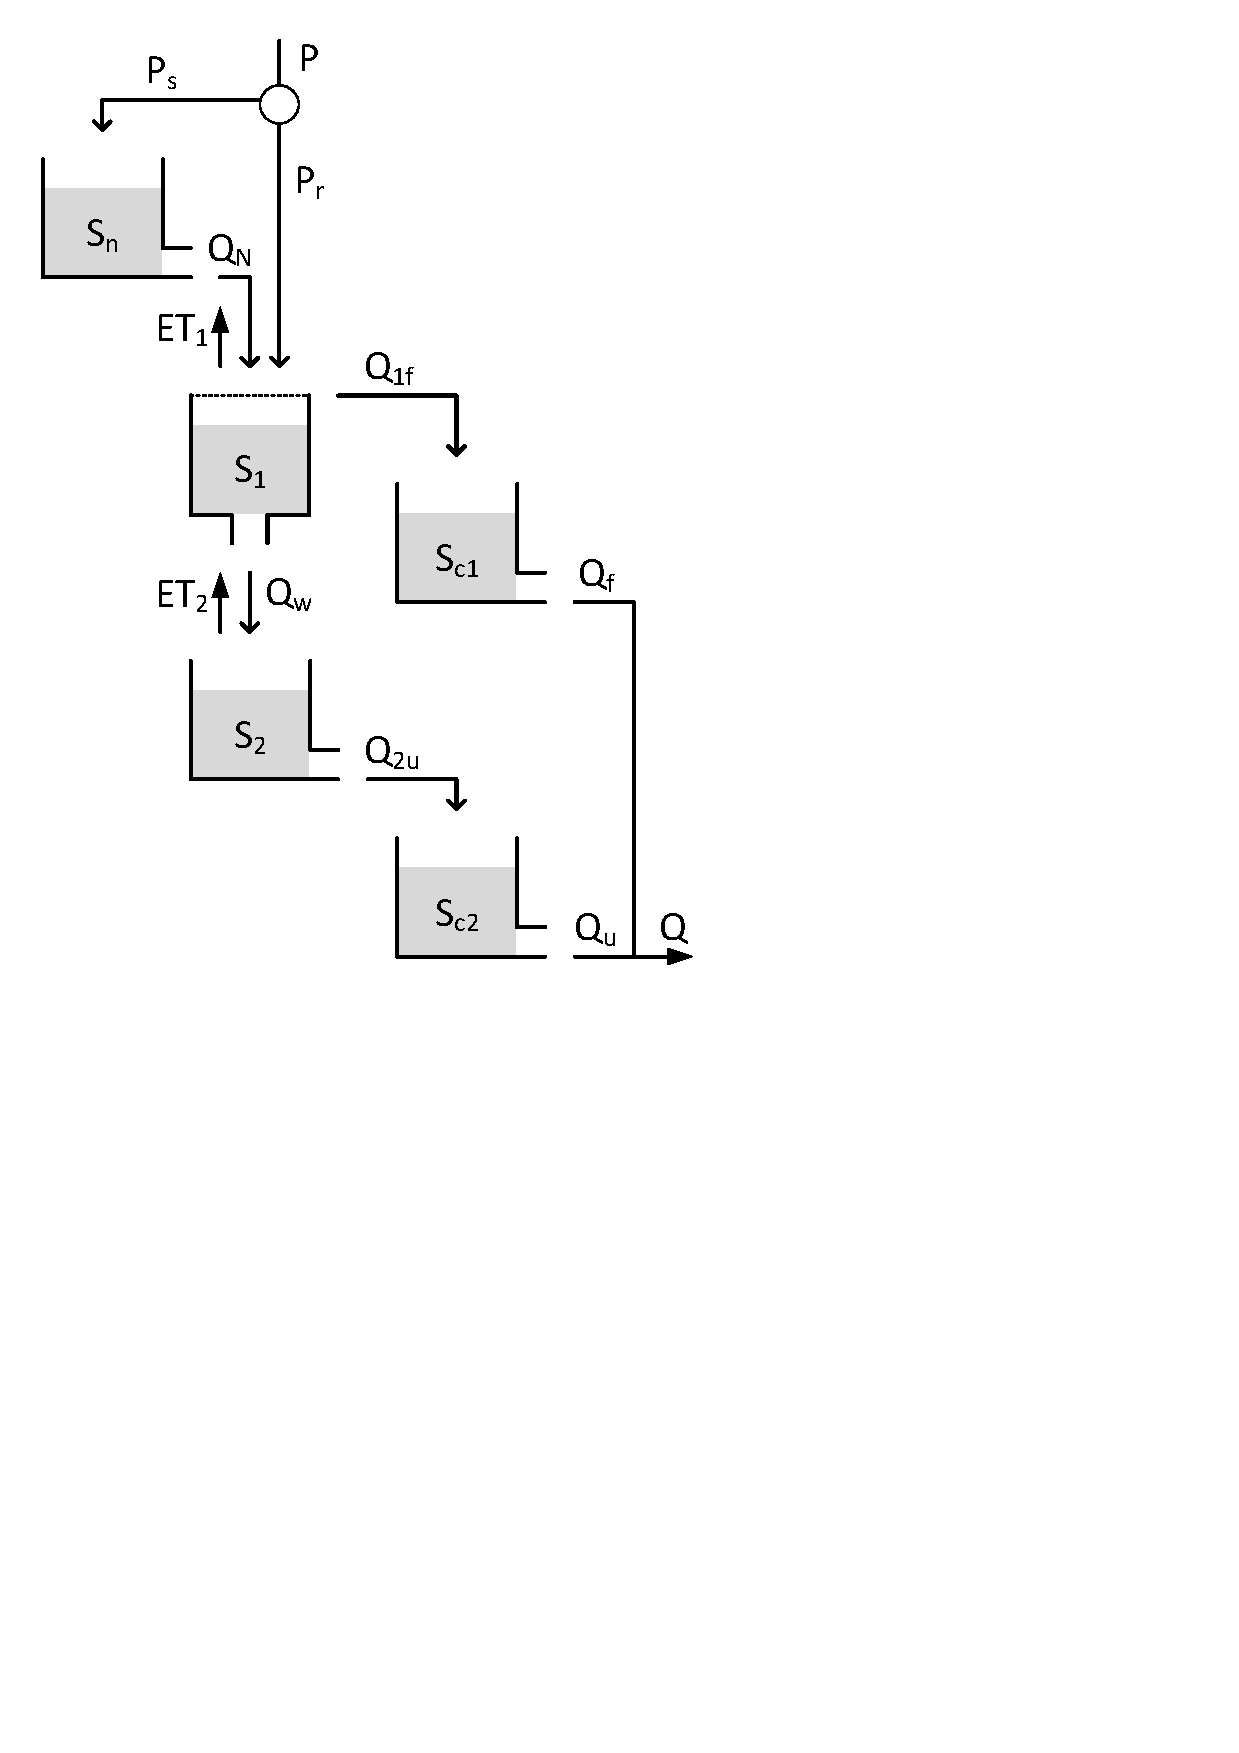
\includegraphics[trim=1cm 13cm 7cm 1cm,width=7cm,keepaspectratio]{./files/30_schematic.pdf}
\caption{Structure of the MOPEX-2 model} \label{fig:30_schematic}
\end{wrapfigure}

\begin{align}
	\frac{dS_n}{dt} &= P_s-Q_{n} \\
	P_s &= \begin{cases}
		P, &\text{if } T \leq T_{crit} \\
		0, & \text{otherwise} \\
	\end{cases} \\
	Q_n &=\begin{cases}
		ddf*(T-T_{crit}), &\text{if } T > T_{crit} \\
		0, & \text{otherwise} \\
	\end{cases}
\end{align}

Where $S_n$ [mm] is the current snow pack. Precipitation occurs as snowfall $P_s$ $[mm/d]$ when current temperature T $[^oC]$ is below threshold $T_{crit}$ $[^oC]$. Snowmelt $Q_N$ $[mm/d]$ occurs when the temperature rises above the threshold temperature and relies in the degree-day factor $dd$ $[mm/^oC/d]$.

\begin{align}
	\frac{dS_1}{dt} &= P_r-ET_1-Q_{1f}-Q_w \\
	P_r &= \begin{cases}
		P, &\text{if } T > T_{crit} \\
		0, & \text{otherwise} \\
	\end{cases} \\
	ET_1 &= \frac{S_1}{S_{b1}}*Ep\\
	Q_{1f} &= \begin{cases}
		P, &\text{if } S_1 \geq S_{b1} \\
		0, & \text{otherwise} \\
	\end{cases} \\
	Q_w &= t_w*S_1
\end{align}

} % end of wrapfigure fix

Where $S_1$ [mm] is the current storage in soil moisture and $P_r$ precipitation as rain $[mm/d]$. Evaporation $ET_1$ $[mm/d]$ depends linearly on current soil moisture, maximum soil moisture $S_{b1}$ [mm] and potential evapotranspiration $E_p$ [mm/d]. Saturation excess flow $Q_{1f}$  $[mm/d]$ occurs when the soil moisture bucket exceeds its maximum capacity. Infiltration to deeper groundwater $Q_w$  $[mm/d]$ depends on current soil moisture and time parameter $t_w$  $[d^{-1}]$.

\begin{align}
	\frac{dS_2}{dt} &= Q_w-ET_2-Q_{2u}\\
	ET_2 &= \frac{S_2}{S_{e}}*Ep\\
	Q_{2u} &= t_u*S_2
\end{align}

Where $S_2$ [mm] is the current groundwater storage, refilled by infiltration from $S_1$. Evaporation $ET_2$ $[mm/d]$ depends linearly on current groundwater and root zone storage capacity $S_e$ [mm]. Leakage to the slow runoff store $Q_{2u}$ $[mm/d]$ depends on current groundwater level and time parameter $t_u$ $[d^{-1}]$. 

\begin{align}
	\frac{dS_{c1}}{dt} &= Q_{1f}-Q_{f}\\
	Q_f &= t_c*S_{c1}
\end{align}

Where $S_{c1}$ [mm] is current storage in the fast flow routing reservoir, refilled by $Q_{1f}$. Routed flow $Q_f$ depends on the mean residence time parameter $t_c$ $[d^{-1}]$.

\begin{align}
	\frac{dS_{c2}}{dt} &= Q_{2u}-Q_{u}\\
	Q_u &= t_c*S_{c2}
\end{align}

Where $S_{c2}$ [mm] is current storage in the slow flow routing reservoir, refilled by $Q_{2u}$. Routed flow $Q_u$ depends on the mean residence time parameter $t_c$ $[d^{-1}]$. Total simulated flow $Q_t$ $[mm/d]$:

\begin{align}
	Q_t &= Q_f + Q_u
\end{align}

\subsubsection{Parameter overview}
% Table generated by Excel2LaTeX from sheet 'Sheet1'
\begin{table}[htbp]
  \centering
    \begin{tabular}{lll}
    \toprule
    Parameter & Unit  & Description \\
    \midrule
    $T_{crit}$ & $^oC$ & Threshold temperature for snowfall and melt \\
    $ddf$ & $mm~^oC^{-1}~d^{-1}$ & Degree-day factor \\
    $S_{b1}$ & $mm$  & Maximum soil moisture storage \\
    $t_w$ & $d^{-1}$ & Runoff coefficient \\
    $t_u$ & $d^{-1}$ & Runoff coefficient \\
    $S_e$ & $mm$  & Maximum groundwater storage capacity \\
    $t_c$ & $d^{-1}$ & Runoff coefficient \\
    \bottomrule
    \end{tabular}%
  \label{tab:addlabel}%
\end{table}%


\section{MOPEX-3 (model ID: 31)}
The MOPEX-3 model (fig.~\ref{fig:31_schematic}) is part of a model improvement study that investigates the relationship between dominant processes and model structures for 197 catchments in the MOPEX database \citep{Ye2012}. It has 5 stores and 8 parameters ($T_{crit}$, $ddf$, $S_{b1}$, $t_w$, $S_{b2}$, $t_u$, $S_e$ and $t_c$). The model aims to represent:

\begin{itemizecompact}
\item Snow accumulation and melt;
\item Saturation excess flow;
\item Infiltration to deeper soil layers;
\item Subsurface-influenced fast flow;
\item A split between fast and slow runoff.
\end{itemizecompact}

\subsection{MARRMoT model name}
m\_31\_mopex3\_8p\_5s \\

% Equations
\subsection{Model equations}

% Model layout figure
{ 																	% This ensures it doesn't warp text further down
\begin{wrapfigure}{l}{6cm}
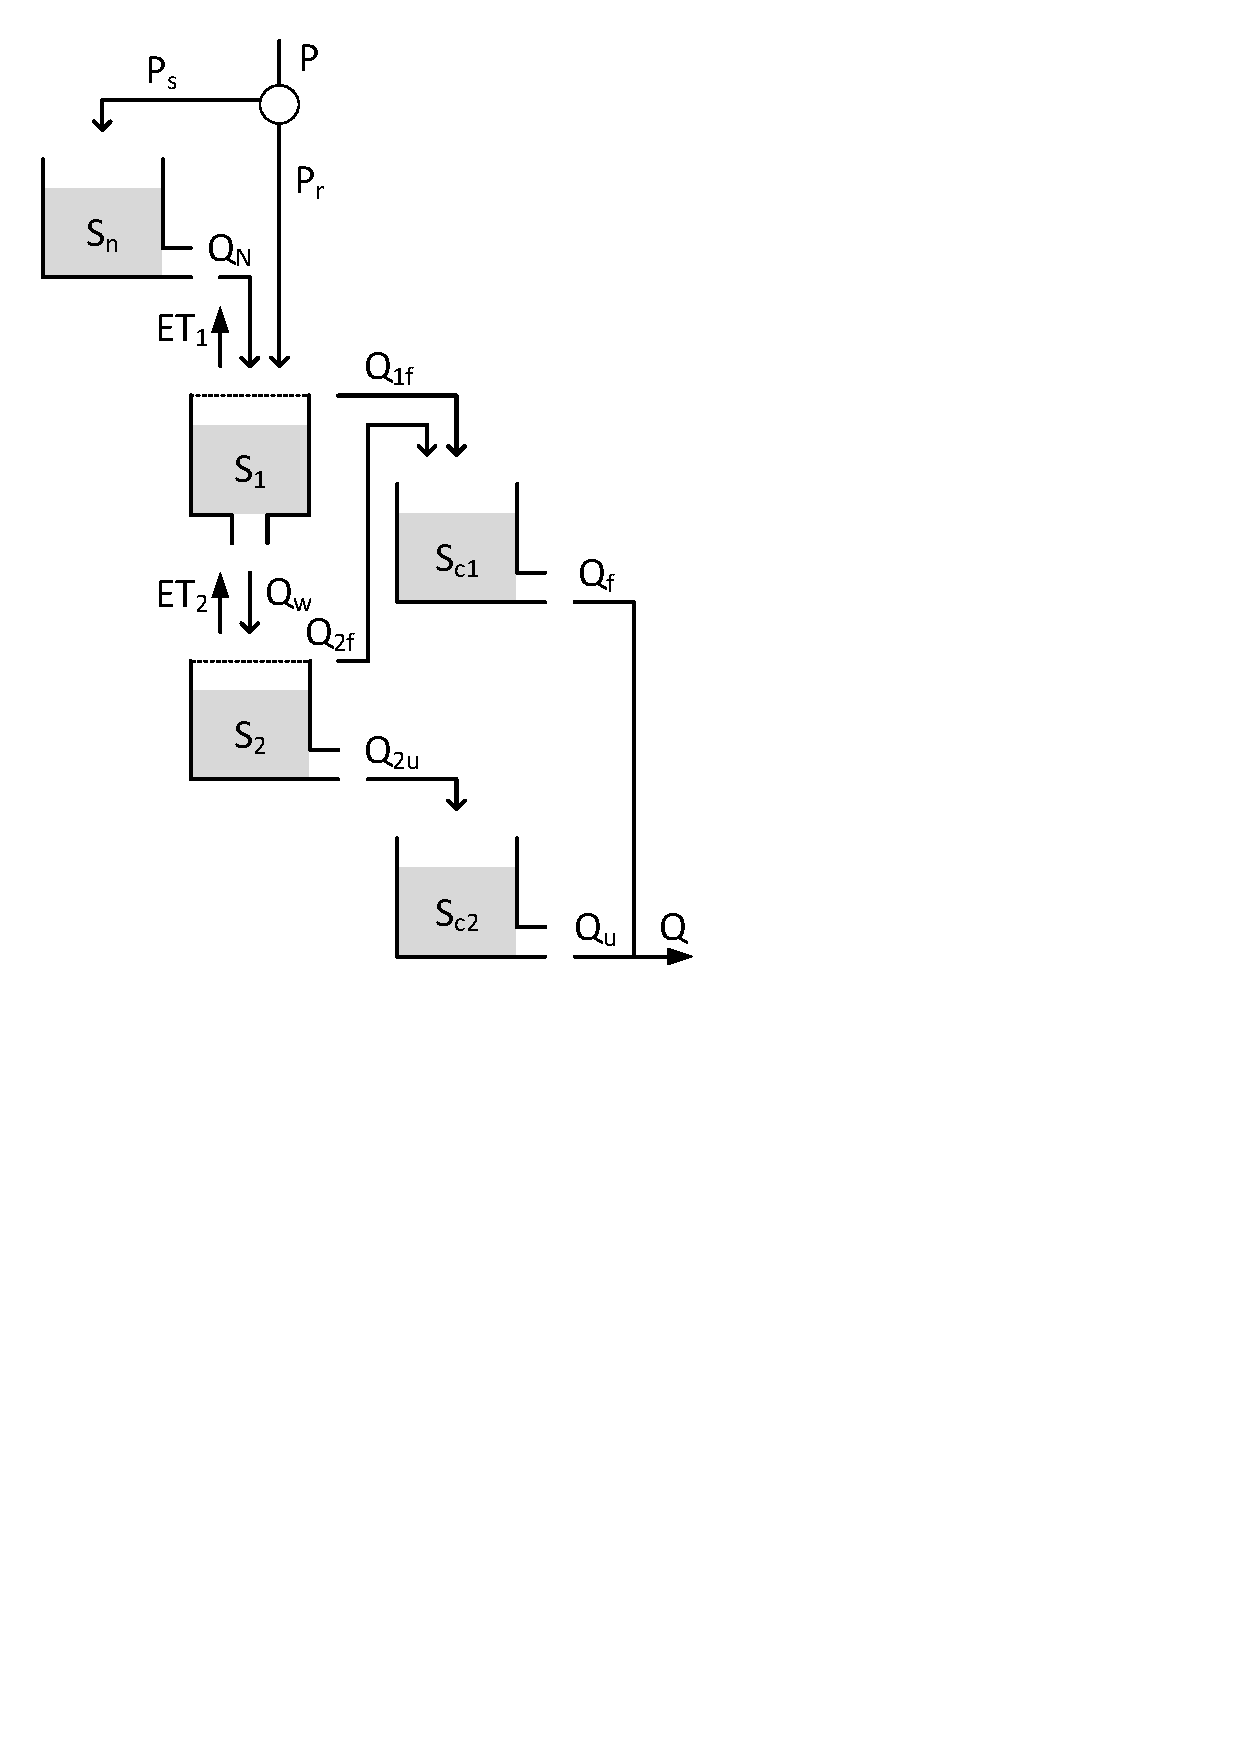
\includegraphics[trim=1cm 13cm 7cm 1cm,width=7cm,keepaspectratio]{./AppA_files/31_schematic.pdf}
\caption{Structure of the MOPEX-3 model} \label{fig:31_schematic}
\end{wrapfigure}

\begin{align}
	\frac{dS_n}{dt} &= P_s-Q_{n} \\
	P_s &= \begin{cases}
		P, &\text{if } T \leq T_{crit} \\
		0, & \text{otherwise} \\
	\end{cases} \\
	Q_n &=\begin{cases}
		ddf*(T-T_{crit}), &\text{if } T > T_{crit} \\
		0, & \text{otherwise} \\
	\end{cases}
\end{align}

Where $S_n$ [mm] is the current snow pack. Precipitation occurs as snowfall $P_s$ $[mm/d]$ when current temperature T $[^oC]$ is below threshold $T_{crit}$ $[^oC]$. Snowmelt $Q_N$ $[mm/d]$ occurs when the temperature rises above the threshold temperature and relies in the degree-day factor $dd$ $[mm/^oC/d]$.

\begin{align}
	\frac{dS_1}{dt} &= P_r-ET_1-Q_{1f}-Q_w \\
	P_r &= \begin{cases}
		P, &\text{if } T > T_{crit} \\
		0, & \text{otherwise} \\
	\end{cases} \\
	ET_1 &= \frac{S_1}{S_{b1}}*Ep\\
	Q_{1f} &= \begin{cases}
		P, &\text{if } S_1 \geq S_{b1} \\
		0, & \text{otherwise} \\
	\end{cases} \\
	Q_w &= t_w*S_1
\end{align}

} % end of wrapfigure fix

Where $S_1$ [mm] is the current storage in soil moisture and $P_r$ precipitation as rain $[mm/d]$. Evaporation $ET_1$ $[mm/d]$ depends linearly on current soil moisture, maximum soil moisture $S_{b1}$ [mm] and potential evapotranspiration $E_p$ [mm/d]. Saturation excess flow $Q_{1f}$  $[mm/d]$ occurs when the soil moisture bucket exceeds its maximum capacity. Infiltration to deeper groundwater $Q_w$  $[mm/d]$ depends on current soil moisture and time parameter $t_w$  $[d^{-1}]$.

\begin{align}
	\frac{dS_2}{dt} &= Q_w-ET_2-Q_{2u} - Q_{2f}\\
	ET_2 &= \frac{S_2}{S_{e}}*Ep\\
	Q_{2u} &= t_u*S_2\\
	Q_{2f} &= \begin{cases}
		Q_w, &\text{if } S_2 \geq S_{b2} \\
		0, & \text{otherwise} \\
	\end{cases}
\end{align}

Where $S_2$ [mm] is the current groundwater storage, refilled by infiltration from $S_1$. Evaporation $ET_2$ $[mm/d]$ depends linearly on current groundwater and root zone storage capacity $S_e$ [mm]. Leakage to the slow runoff store $Q_{2u}$ $[mm/d]$ depends on current groundwater level and time parameter $t_u$ $[d^{-1}]$. When the store reaches maximum capacity $S_{b2}$ [mm], excess flow $Q_{2f}$ $[mm/d]$ is routed towards the fast response routing store.

\begin{align}
	\frac{dS_{c1}}{dt} &= Q_{1f}+Q_{2f}-Q_{f}\\
	Q_f &= t_c*S_{c1}
\end{align}

Where $S_{c1}$ [mm] is current storage in the fast flow routing reservoir, refilled by $Q_{1f}$ and $Q_{2f}$. Routed flow $Q_f$ depends on the mean residence time parameter $t_c$ $[d^{-1}]$.

\begin{align}
	\frac{dS_{c2}}{dt} &= Q_{2u}-Q_{u}\\
	Q_u &= t_c*S_{c2}
\end{align}

Where $S_{c2}$ [mm] is current storage in the slow flow routing reservoir, refilled by $Q_{2u}$. Routed flow $Q_u$ depends on the mean residence time parameter $t_c$ $[d^{-1}]$. Total simulated flow $Q_t$ $[mm/d]$:

\begin{align}
	Q_t &= Q_f + Q_u
\end{align}

\subsection{Parameter overview}
% Table generated by Excel2LaTeX from sheet 'Sheet1'
\begin{table}[htbp]
  \centering
    \begin{tabular}{lll}
    \toprule
    Parameter & Unit  & Description \\
    \midrule
    $T_{crit}$ & $^oC$ & Threshold temperature for snowfall and melt \\
    $ddf$ & $mm~^oC^{-1}~d^{-1}$ & Degree-day factor \\
    $S_{b1}$ & $mm$  & Maximum soil moisture storage \\
    $t_w$ & $d^{-1}$ & Runoff coefficient \\
    $S_{b2}$ & $mm$  & Maximum deep storage \\
    $t_u$ & $d^{-1}$ & Runoff coefficient \\
    $S_e$ & $mm$  & Maximum groundwater storage capacity \\
    $t_c$ & $d^{-1}$ & Runoff coefficient \\
    \bottomrule
    \end{tabular}%
  \label{tab:addlabel}%
\end{table}%


\subsection{MOPEX-4 (model ID: 32)}
The MOPEX-4 model (fig.~\ref{fig:32_schematic}) is part of a model improvement study that investigates the relationship between dominant processes and model structures for 197 catchments in the MOPEX database \citep{Ye2012}. It has 5 stores and 10 parameters ($T_{crit}$, $ddf$, $S_{b1}$, $t_w$, $I_{\alpha}$, $I_{s}$, $S_{b2}$, $t_u$, $S_e$ and $t_c$). The original model relies on observations of Leaf Area Index and a calibrated interception fraction. \citet{Liang1994} show typical Leaf Area Index time series, and a sinusoidal function is a reasonable approximation of this. Therefore, the model is slightly modified to use a calibrated sinusoidal function, so that the data input requirements for MOPEX-4 are consistent with other models.  The model aims to represent:

\begin{itemizecompact}
\item Snow accumulation and melt;
\item Time-varying interception;
\item Saturation excess flow;
\item Infiltration to deeper soil layers;
\item A split between fast and slow runoff.
\end{itemizecompact}

\subsubsection{File names}
\begin{tabular}{@{}ll}
Model: &m\_32\_mopex4\_10p\_5s \\
Parameter ranges: &m\_32\_mopex4\_10p\_5s\_parameter\_ ranges \\
\end{tabular}

% Equations
\subsubsection{Model equations}

% Model layout figure
{ 																	% This ensures it doesn't warp text further down
\begin{wrapfigure}{l}{6cm}
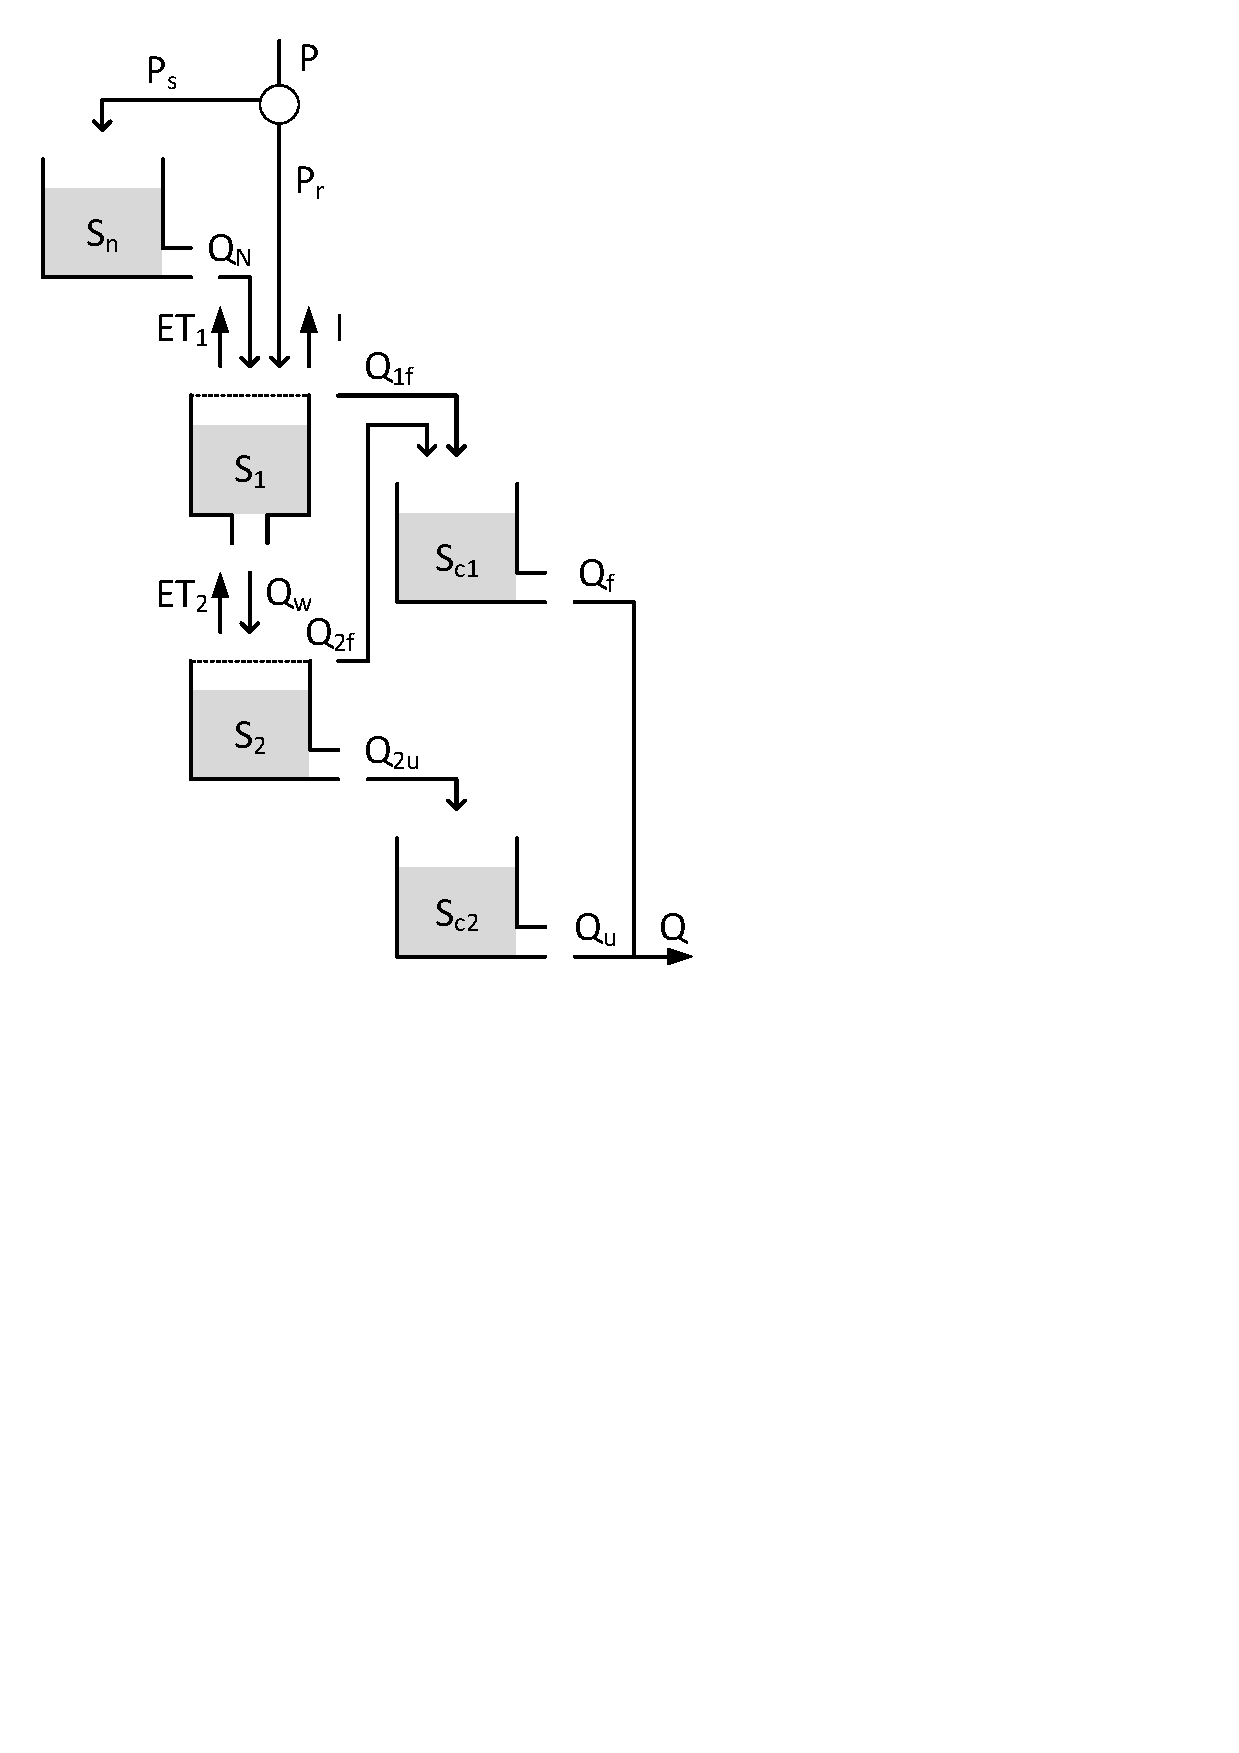
\includegraphics[trim=1cm 13cm 7cm 1cm,width=7cm,keepaspectratio]{./files/32_schematic.pdf}
\caption{Structure of the MOPEX-4 model} \label{fig:32_schematic}
\end{wrapfigure}

\begin{align}
	\frac{dS_n}{dt} &= P_s-Q_{n} \\
	P_s &= \begin{cases}
		P, &\text{if } T \leq T_{crit} \\
		0, & \text{otherwise} \\
	\end{cases} \\
	Q_n &=\begin{cases}
		ddf*(T-T_{crit}), &\text{if } T > T_{crit} \\
		0, & \text{otherwise} \\
	\end{cases}
\end{align}

Where $S_n$ [mm] is the current snow pack. Precipitation occurs as snowfall $P_s$ $[mm/d]$ when current temperature T $[^oC]$ is below threshold $T_{crit}$ $[^oC]$. Snowmelt $Q_N$ $[mm/d]$ occurs when the temperature rises above the threshold temperature and relies in the degree-day factor $dd$ $[mm/^oC/d]$.

} % end of wrapfigure fix
\vspace{5cm}

\begin{align}
	\frac{dS_1}{dt} &= P_r-ET_1-I-Q_{1f}-Q_w \\
	P_r &= \begin{cases}
		P, &\text{if } T > T_{crit} \\
		0, & \text{otherwise} \\
	\end{cases} \\
	ET_1 &= \frac{S_1}{S_{b1}}*Ep\\
	I &=max\left(0,I_{\alpha} + (1-I_{\alpha})cos\left(2\pi\frac{t-I_{s}}{t_{max}}\right)\right)*P_r\\
	Q_{1f} &= \begin{cases}
		P, &\text{if } S_1 \geq S_{b1} \\
		0, & \text{otherwise} \\
	\end{cases} \\
	Q_w &= t_w*S_1
\end{align}

Where $S_1$ [mm] is the current storage in soil moisture and $P_r$ precipitation as rain $[mm/d]$. Evaporation $ET_1$ $[mm/d]$ depends linearly on current soil moisture, maximum soil moisture $S_{b1}$ [mm] and potential evapotranspiration $E_p$ [mm/d]. Interception $I$ $[mm/d]$ depends on the mean intercepted fraction $I_{\alpha}$ [-],  the maximum Leaf Area Index timing $I_{s}$ [d] and the length of the seasonal cycle $t_{max}$ [d] (usually set at 365 days). Saturation excess flow $Q_{1f}$  $[mm/d]$ occurs when the soil moisture bucket exceeds its maximum capacity. Infiltration to deeper groundwater $Q_w$  $[mm/d]$ depends on current soil moisture and time parameter $t_w$  $[d^{-1}]$.

\begin{align}
	\frac{dS_2}{dt} &= Q_w-ET_2-Q_{2u} - Q_{2f}\\
	ET_2 &= \frac{S_2}{S_{e}}*Ep\\
	Q_{2u} &= t_u*S_2\\
	Q_{2f} &= \begin{cases}
		Q_w, &\text{if } S_2 \geq S_{b2} \\
		0, & \text{otherwise} \\
	\end{cases}
\end{align}

Where $S_2$ [mm] is the current groundwater storage, refilled by infiltration from $S_1$. Evaporation $ET_2$ $[mm/d]$ depends linearly on current groundwater and root zone storage capacity $S_e$ [mm]. Leakage to the slow runoff store $Q_{2u}$ $[mm/d]$ depends on current groundwater level and time parameter $t_u$ $[d^{-1}]$. When the store reaches maximum capacity $S_{b2}$ [mm], excess flow $Q_{2f}$ $[mm/d]$ is routed towards the fast response routing store.

\begin{align}
	\frac{dS_{c1}}{dt} &= Q_{1f}+Q_{2f}-Q_{f}\\
	Q_f &= t_c*S_{c1}
\end{align}

Where $S_{c1}$ [mm] is current storage in the fast flow routing reservoir, refilled by $Q_{1f}$ and $Q_{2f}$. Routed flow $Q_f$ depends on the mean residence time parameter $t_c$ $[d^{-1}]$.

\begin{align}
	\frac{dS_{c2}}{dt} &= Q_{2u}-Q_{u}\\
	Q_u &= t_c*S_{c2}
\end{align}

Where $S_{c2}$ [mm] is current storage in the slow flow routing reservoir, refilled by $Q_{2u}$. Routed flow $Q_u$ depends on the mean residence time parameter $t_c$ $[d^{-1}]$. Total simulated flow $Q_t$ $[mm/d]$:

\begin{align}
	Q_t &= Q_f + Q_u
\end{align}

\subsubsection{Parameter overview}
% Table generated by Excel2LaTeX from sheet 'Sheet1'
\begin{table}[htbp]
  \centering
    \begin{tabular}{lll}
    \toprule
    Parameter & Unit  & Description \\
    \midrule
    $T_{crit}$ & $^oC$ & Threshold temperature for snowfall and melt \\
    $ddf$ & $mm~^oC^{-1}~d^{-1}$ & Degree-day factor \\
    $S_{b1}$ & $mm$  & Maximum soil moisture storage \\
    $t_w$ & $d^{-1}$ & Runoff coefficient \\
    $I_{\alpha}$ & $-$   & Mean intercepted fraction of precipitation \\
    $I_{s}$ & $d$   & Timing of peak interception capacity \\
    $S_{b2}$ & $mm$  & Maximum deep storage \\
    $t_u$ & $d^{-1}$ & Runoff coefficient \\
    $S_e$ & $mm$  & Maximum groundwater storage capacity \\
    $t_c$ & $d^{-1}$ & Runoff coefficient \\
    \bottomrule
    \end{tabular}%
  \label{tab:addlabel}%
\end{table}%

\subsection{SACRAMENTO model (model ID: 33)}
The SACRAMENTO model (fig.~\ref{fig:33_schematic}) is part of an ongoing model development project by the National Weather Service, which started several decades ago \citep{Burnash1995,NationalWeatherService2005}. The documentation mentions a specific order of flux computations. For consistency with other models, here all fluxes are computed simultaneously. It has 5 stores and 13 parameters ($PCTIM$, $UZTWM$, $UZFWM$, $k_{uz}$, $PBASE$, $ZPERC$, $REXP$, $LZTWM$, $LZFWPM$, $LZFWSM$, $PFREE$, $k_{lzp}$ and $k_{lzs}$). The model also uses several coefficients derived from the calibration parameters \citep{Koren2000}: $PBASE$ and $ZPERC$. The model aims to represent:

\begin{itemizecompact}
\item Impervious and direct runoff;
\item Within soil division of water storage between tension and free water;
\item Surface runoff, interflow and percolation to deeper soil layers;
\item Multiple baseflow processes.
\end{itemizecompact}

\subsubsection{File names}
\begin{tabular}{@{}ll}
Model: &m\_33\_sacramento\_11p\_5s \\
Parameter ranges: &m\_33\_sacramento\_11p\_5s\_parameter\_ ranges \\
\end{tabular}

% Equations
\subsubsection{Model equations}

% Model layout figure
{ 																	% This ensures it doesn't warp text further down
\begin{wrapfigure}{l}{6cm}
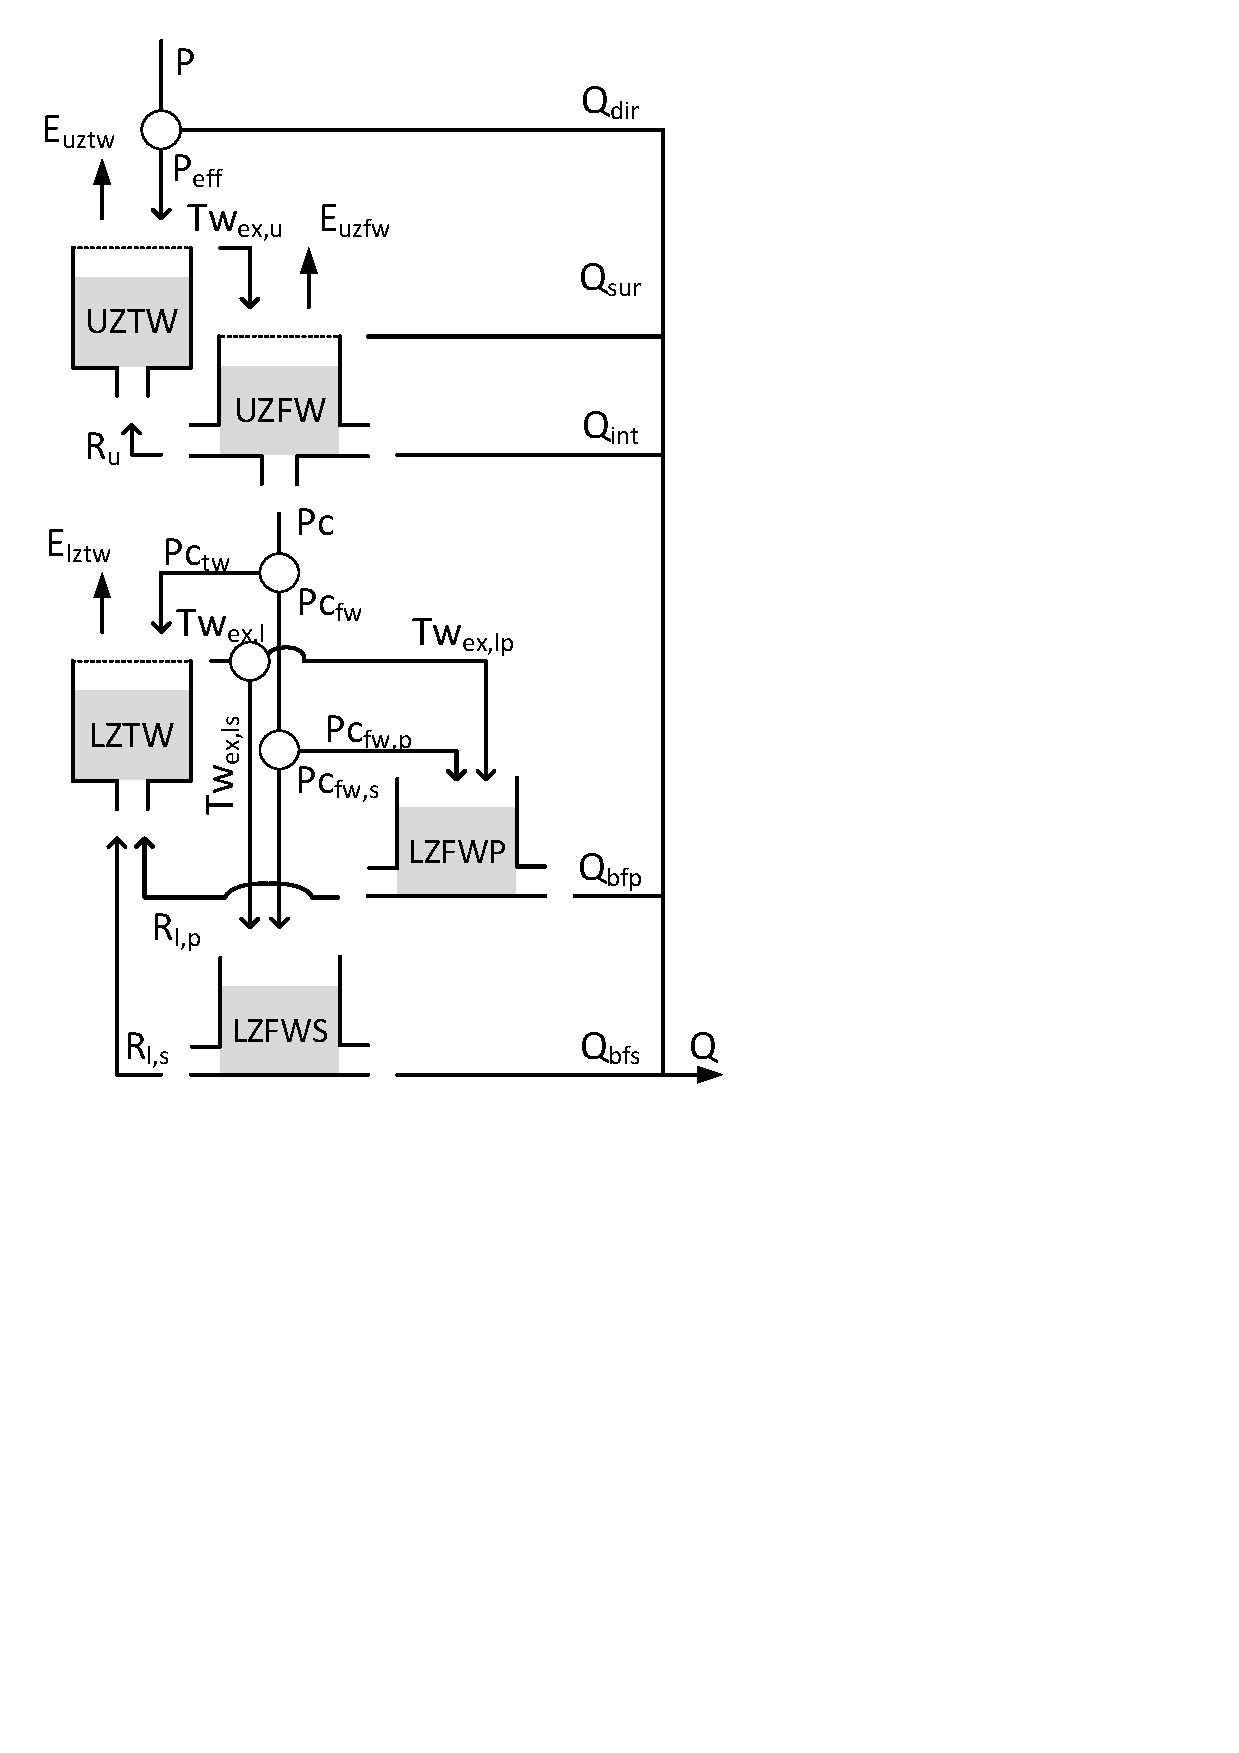
\includegraphics[trim=1cm 11cm 7cm 1cm,width=7cm,keepaspectratio]{./files/33_schematic.pdf}
\caption{Structure of the SACRAMENTO model} \label{fig:33_schematic}
\end{wrapfigure}

\begin{align}
	\frac{dUZTW}{dt} &= P_{eff} + R_u -E_{uztw}-Tw_{ex,u} \\
	P_{eff} &= (1-PCTIM)*P\\
	Q_{dir} &= PCTIM*P\\
	R_u &= \begin{cases} 
		\begin{aligned}
			\frac{UZTWM*UZFW-UZFWM*UZTW}{UZTWM+UZFWM}, \\	
			\text{if } \frac{UZTW}{UZTWM} < \frac{UZFW}{UZFWM} \\
		\end{aligned}\\
		0, \quad \text{otherwise} \\
	\end{cases}\\
	E_{uztw} &= \frac{UZTW}{UZTWM}*E_p\\
	Tw_{ex,u} &= \begin{cases}
		P_{eff}, &\text{if } UZTW = UZTWM \\
		0, & \text{otherwise} \\
	\end{cases} 
\end{align}

Where $UZTW$ [mm] is upper zone tension water, refilled by effective precipitation 

} % end of wrapfigure fix

\noindent$P_{eff}$ $[mm/d]$ and redistribution of free water $R_u$  $[mm/d]$, and is drained by evaporation $E_{uztw}$ $[mm/d]$ and tension water excess $Tw_{ex,u}$ $[mm/d]$.
$P_{eff}$ is the fraction $(1-PCTIM)$ [-] of precipitation $P$ that does not fall on impervious fraction $PCTIM$ [-].
$Q_{dir}$ $[mm/d]$ is the corresponding fraction direct runoff.
$R_u$ is only active when the relative deficit in tension water is greater than that in free water, and rebalances the available water in the upper zone. This uses the current storages, $UZTW$ and $UZFW$, and maximum storages, $UZTWM$ [mm] and $UZFWM$ [mm], of tension and free water stores respectively.
Evaporation is determined with a linear relation between available, maximum upper zone tension storage and potential evapotranspiration $E_p$ [mm/d].
$Tw_{ex,u}$ occurs only when the store is at maximum capacity.



\begin{align}
	\frac{dUZFW}{dt} &= Tw_{ex,u} - E_{uzfw} - Q_{sur} - Q_{int} - Pc - R_u \\
	E_{uzfw} &= \begin{cases}
		E_p-E_{uztw}, &\text{if } UZFW > 0 ~\&~ E_p>E_{uztw} \\
		0, & \text{otherwise} \\
	\end{cases}\\
	Q_{sur} &= \begin{cases}
		Tw_{ex,u}, &\text{if } UZFW = UZFWM \\
		0, & \text{otherwise} \\
	\end{cases}\\
	Q_{int} &= k_{uz} * UZFW\\
	Pc &= Pc_{demand} *\frac{UZFW}{UZFWM}\\
	Pc_{demand} &= PBASE*\left(1+ZPERC*\left(\frac{\sum{LZ_{deficiency}}}{\sum{LZ_{capacity}}}\right)^{1+REXP}\right)\\
	LZ_{deficiency} &= [LZTWM-LZTW]+[LZFWPM-LZWFP]+[LZFWSM-LZFWS]\\
	LZ_{capacity} &= LZTWM+LZFWPM+LZFWSM
\end{align}

Where $UZFW$ [mm] is upper zone free water, refilled by excess water $Tw_{ex,u}$ that can not be stored as tension water, and drained by evaporation  $E_{uzfw}$ $[mm/d]$, surface runoff $Q_{sur}$ $[mm/d]$, interflow $Q_{int}$ $[mm/d]$, and percolation to deeper groundwater $Pc$ $[mm/d]$.
Evaporative demand unmet by the upper tension water store is taken from upper free water storage at the potential rate.
$Q_{sur}$ occurs only when the store is at maximum capacity $UZFWM$ [mm].
$Q_{int}$ uses time coefficient $k_{uz}$ $[d^{-1}]$ to simulate interflow.
Percolation $Pc$ is calculated as a balance between the fraction water availability in upper zone free storage, and demand from the lower zone $Pc_{demand}$. The demand can be between a base percolation rate $PBASE$ $[mm/d]$ and an upper limit of $ZPERC$ [-] times $PBASE$. This demand is scaled by the relative size of lower zone moisture deficiencies, expressed as the ratio between total deficiency and maximum lower zone storage. $LZTWM$ [mm], $LZFWP$ [mm], $LZFWS$ [mm] are the maximum capacity of the lower zone tension store, primary free water store and supplemental free water store respectively. The lower zone percolation demand is potentially non-linear through exponent $REGX$ [-]. $PBASE$ is calculated as $k_{lzp}*LZFWPM+K_{lzs}*LZFWSM$.

\begin{align}
	\frac{dLZTW}{dt} &= Pc_{tw} + R_{l,p} + R_{l,s} - E_{lztw} - Tw_{ex,l} \\
	Pc_{tw} &= (1-PFREE)*Pc\\
	R_{l,p} &= \begin{cases}
		\begin{aligned}
		LZFWPM*\frac{-LZTW(LZFWPM+LZFWSM)+LZTWM(LZWFP+LZWFS)}{(LZFWPM+LZFWSM)(LZTWM+LZFWPM+LZFWSM)}, \\
				\text{if } \frac{LZTW}{LZTWM} < \frac{LZFWP+LZFWS}{LZFWPM+LZFWSM}\\
		\end{aligned}\\
		0, \quad \text{otherwise} \\
	\end{cases}\\	
	R_{l,s} &= \begin{cases}
		\begin{aligned}
		LZFWSM*\frac{-LZTW(LZFWPM+LZFWSM)+LZTWM(LZWFP+LZWFS)}{(LZFWPM+LZFWSM)(LZTWM+LZFWPM+LZFWSM)}, \\
			\text{if } \frac{LZTW}{LZTWM} < \frac{LZFWP+LZFWS}{LZFWPM+LZFWSM}\\
		\end{aligned}\\
		0, \quad \text{otherwise} \\
	\end{cases}\\	
	E_{lztw} &= \begin{cases}
		\left(E_p-E_{uztw}-E_{uzfw}\right)*\frac{LZTW}{UZTWM+LZTWM}, &\text{if } LZTW > 0 ~\&~ E_p > (E_{uztw}+E_{uzfw}) \\
		0, & \text{otherwise} \\
	\end{cases}\\
	Tw_{ex,l} &= \begin{cases}
		Pc_{tw}, &\text{if } LZTW = LZTWM \\
		0, & \text{otherwise} \\
	\end{cases}
\end{align}

Where $ LZTW$ [mm] is lower zone tension water, refilled by percolation $Pc_{tw}$ $[mm/d]$ and drained by evaporation $E_{lztw}$ $[mm/d]$ and tension water excess $Tw_{ex,l}$ $[mm/d]$.
Evaporative demand unmet b the upper zone can be satisfied from the lower zone tension water store, scaled by the current lower zone storage relative to total tension zone storage.
Both $R_{l,p}$ and $R_{l,s}$ are only active when the relative deficit in tension water is greater than that in free water, and rebalances the available water in the lower zone. This uses the current storages, $LZTW$, $LZFWP$ and $LZFWS$, and maximum storages, $LZTWM$ [mm], $LZFWPM$ [mm] and $LZFWSM$ [mm], of the tension and free water stores respectively.
$Pc_{tw}$ is the fraction $(1-PFREE)$ [-] of percolation $Pc$ that does not go into free storage.
$Tw_{ex,l}$ occurs only when the store is at maximum capacity $LZTWM$ [mm].

\begin{align}
	\frac{dLZFWP}{dt} &= Pc_{fw,p} + Tw_{ex,lp} - Q_{bfp} \\
	Pc_{fw,p} &= \left[\frac{LZFWPM-LZFWP}{LZFWPM\left(\frac{LZFWPM-LZFWP}{LZFWPM}+\frac{LZFWSM-LZFWS}{LZFWSM}\right)}\right]*\left(PFREE*Pc\right)\\
	Tw_{ex,lp} &= \left[\frac{LZFWPM-LZFWP}{LZFWPM\left(\frac{LZFWPM-LZFWP}{LZFWPM}+\frac{LZFWSM-LZFWS}{LZFWSM}\right)}\right]*Tw_{ex,l}\\
	Q_{bfp} &= k_{lzp}*LZFWP
\end{align}

Where $LZFWP$ [mm] is current storage in the primary lower zone free water store, refilled by excess tension water $TW_{ex,lp}$ $[mm/d]$ and percolation $Pc_{fw,p}$ $[mm/d]$ and drained by primary baseflow $Q_{bfp}$ $[mm/d]$.
Refilling of both lower zone free water stores (primary and supplemental) is divided between the two based on their relative, scaled moisture deficiency.
Percolation from the upper zone $Pc_{fw,p}$ is scaled according to the relative current moisture deficit $\frac{LZFWPM-LZFWP}{LZFWM}$ compared to the total relative deficit in the lower free water stores $\left(\frac{LZFWPM-LZFWP}{LZFWPM}+\frac{LZFWSM-LZFWS}{LZFWSM}\right)$.
$Tw_{ex,lp}$ is a similarly scaled part of $Tw_{ex,l}$.
$Q_{bfp}$ uses time parameter $K_{lzp}$ $[d^{-1}]$ to estimate primary baseflow.

\begin{align}
	\frac{dLZFWS}{dt} &= Pc_{fw,s} + Tw_{ex,ls} - Q_{bfs} \\
	Pc_{fw,s} &= \left[\frac{LZFWSM-LZFWS}{LZFWSM\left(\frac{LZFWPM-LZFWP}{LZFWPM}+\frac{LZFWSM-LZFWS}{LZFWSM}\right)}\right]*\left(PFREE*Pc\right)\\
	Tw_{ex,ls} &= \left[\frac{LZFWSM-LZFWS}{LZFWSM\left(\frac{LZFWPM-LZFWP}{LZFWPM}+\frac{LZFWSM-LZFWS}{LZFWSM}\right)}\right]*Tw_{ex,l}\\
	Q_{bfs} &= k_{lzs}*LZFWS
\end{align}

Where $LZFWS$ [mm] is current storage in the supplemental free water lower zone store, refilled by excess tension water $TW_{ex,ls}$ $[mm/d]$ and percolation $Pc_{fw,s}$ $[mm/d]$, and drained by supplemental baseflow $Q_{bfs}$ $[mm/d]$. 
$Pc_{fw,s}$ is determined based on relative deficits in the lower zone free stores, as is $Tw_{ex,ls}$.
$Q_{bfs}$ uses time parameter $K_{lzs}$ $[d^{-1}]$ to estimate supplementary baseflow. Total simulated outflow:

\begin{align}
	Q_t &= Q_{dir} + Q_{sur} + Q_{int} + Q_{bfp} + Q_{bfs}
\end{align}

\newpage
\subsubsection{Parameter overview}
% Table generated by Excel2LaTeX from sheet 'Sheet1'
\begin{table}[htbp]
  \centering
    \begin{tabular}{lll}
    \toprule
    Parameter & Unit  & Description \\
    \midrule
    $PCTIM$ & $-$   & Fraction impervious area \\
    $UZTWM$ & $mm$  & Maximum upper zone tension water storage \\
    $UZFWM$ & $mm$  & Maximum upper zone free water storage \\
    $k_{uz}$ & $d^{-1}$ & Runoff coefficient \\
    $PBASE$ & $mm~d^{-1}$ & Base percolation rate \\
    $ZPERC$ & $-$   & Maximum percolation rate as multiple of $ZPERC$ \\
    $REXP$ & $-$   & Percolation non-linearity parameter \\
    $LZTWM$ & $mm$  & Maximum lower zone tension water storage \\
    $LZFWPM$ & $mm$  & Maximum lower zone primary free water storage \\
    $LZFWSM$ & $mm$  & Maximum lower zone secondary free water storage \\
    $PFREE$ & $-$   & Fraction of percolation to free storage \\
    $k_{lzp}$ & $d^{-1}$ & Runoff coefficient \\
    $k_{lzs}$ & $d^{-1}$ & Runoff coefficient \\
    \bottomrule
    \end{tabular}%
  \label{tab:addlabel}%
\end{table}%


\subsection{FLEX-IS (model ID: 34)}
The FLEX-IS model (fig.~\ref{fig:34_schematic}) is a combination of the FLEX-B model expanded with an interception (I) routine \citep{Fenicia2008} and a snow (S) module \citep{Nijzink2016}. It has 5 stores and 12 parameters ($TT$, $ddf$, $I_{max}$, $UR_{max}$, $\beta$, $L_p$, $Perc_{max}$, $D$, $N_{lag,f}$, $N_{lag,s}$, $K_f$ and $K_s$). The model aims to represent:

\begin{itemizecompact}
\item Snow accumulation and melt;
\item Interception by vegetation;
\item Infiltration and saturation excess flow based on a distribution of different soil depths;
\item A split between fast saturation excess flow and preferential recharge to a slow store;
\item Percolation from the unsaturated zone to a slow runoff store.
\end{itemizecompact}

\subsubsection{File names}
\begin{tabular}{@{}ll}
Model: &m\_34\_flexis\_12p\_5s \\
Parameter ranges: &m\_34\_flexis\_12p\_5s\_parameter\_ ranges \\
\end{tabular}

% Equations
\subsubsection{Model equations}

% Model layout figure
{ 																	% This ensures it doesn't warp text further down
\begin{wrapfigure}{l}{7cm}
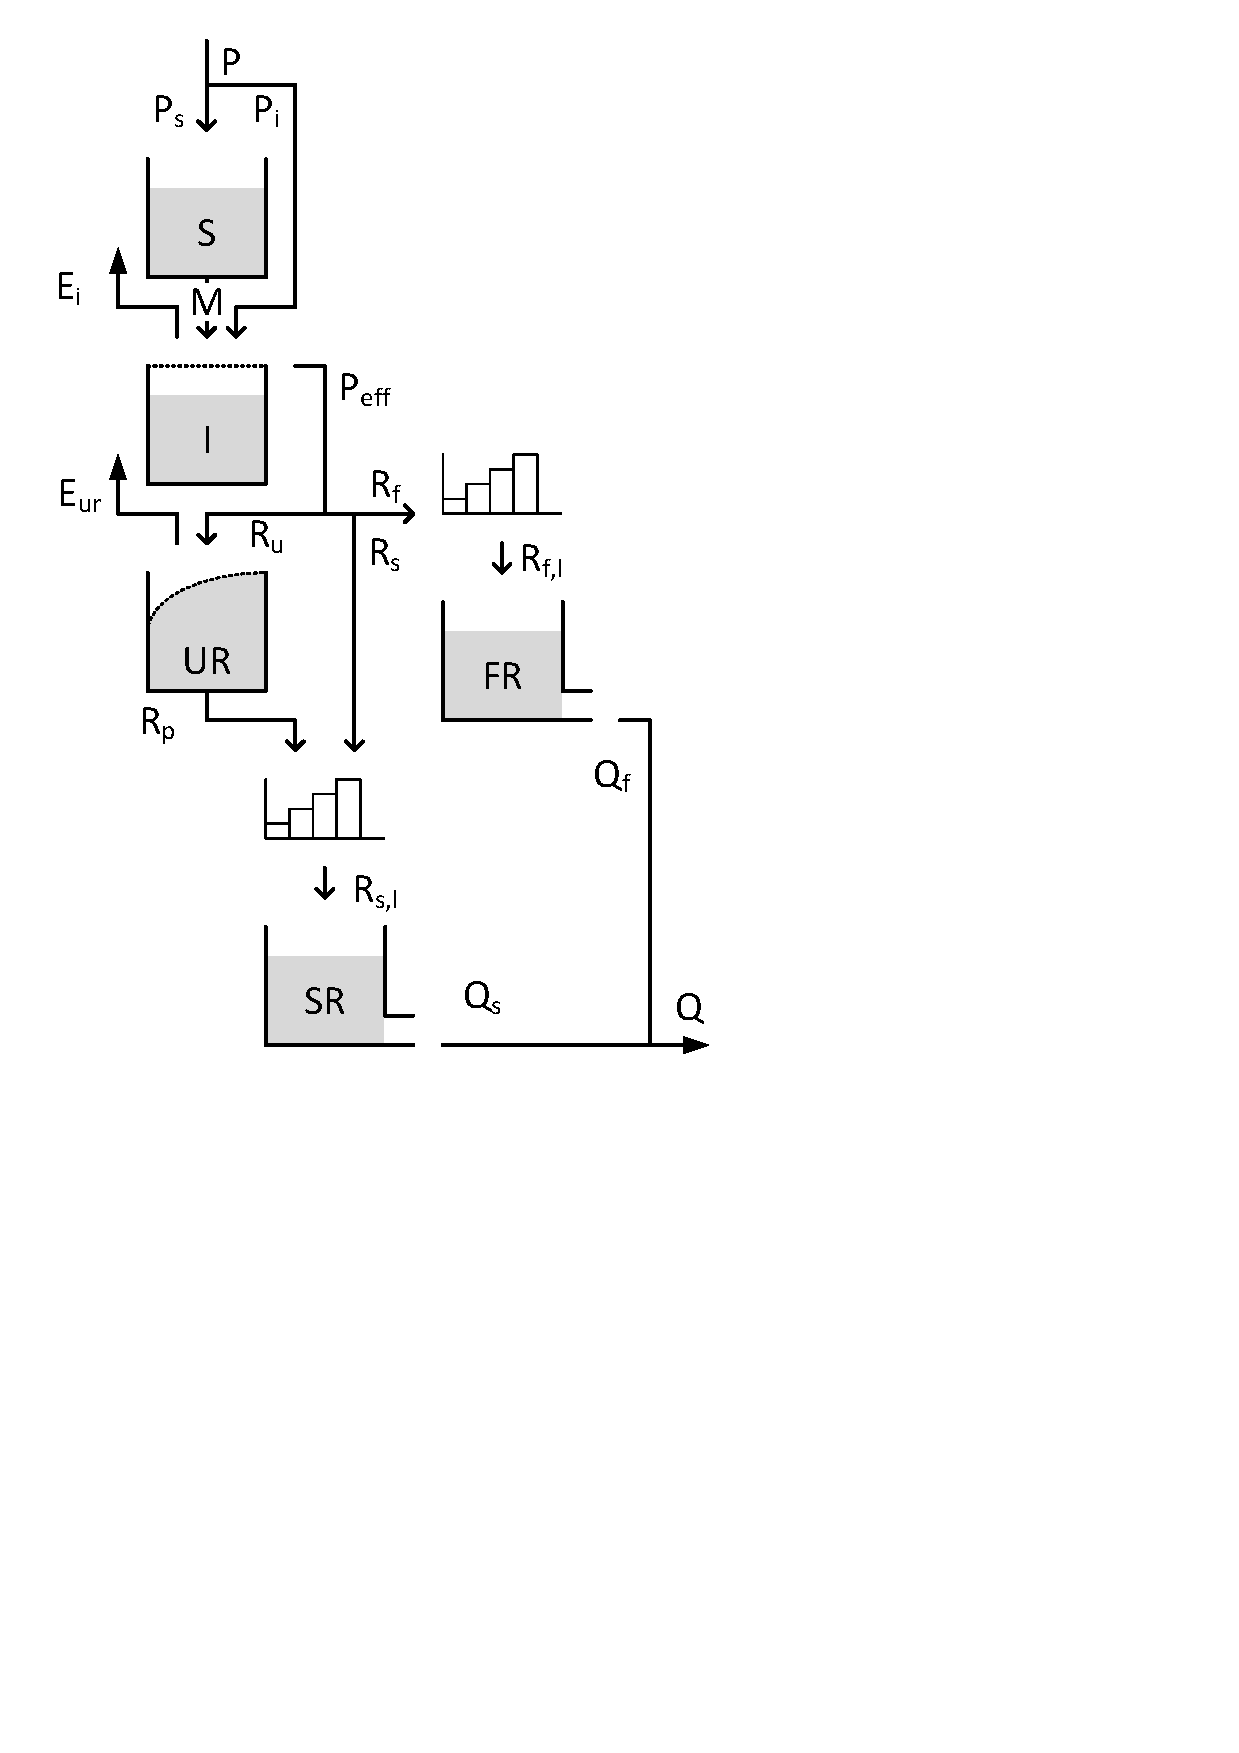
\includegraphics[trim=1cm 12cm 7cm 1cm,width=7cm,keepaspectratio]{./files/34_schematic.pdf}
\caption{Structure of the FLEX-IS model} \label{fig:34_schematic}
\end{wrapfigure}

\begin{align}
	\frac{dS}{dt} &= P_s-M \\
	P_s &= \begin{cases}
		P, &\text{if } T \leq TT \\
		0, & \text{otherwise} \\
	\end{cases} \\
	M &= 
	\begin{cases}
		ddf*(T - TT), & \text{if } T \geq TT \\
		0, & \text{otherwise}
	\end{cases}
\end{align}

Where S [mm] is the current snow storage, $P_s$ the precipitation that falls as snow [mm/d], M the snowmelt $[mm/d]$ based on a degree-day factor (ddf, [mm/\degree C/d]) and threshold temperature for snowfall and snowmelt (TT, [\degree C]).


\begin{align}
	\frac{dI}{dt} &= P_I + M - E_I  - P_{eff}\\
	P_i &= \begin{cases}
		P, &\text{if } T > TT \\
		0, & \text{otherwise} \\
	\end{cases} \\
	E_i &= \begin{cases}
		E_p, &\text{if } I > 0 \\
		0, &\text{otherwise} \\
	\end{cases} \\
	P_{eff} &= \begin{cases}
		P_i, &\text{if } I = I_{max}\\
		0, &\text{otherwise}\\
	\end{cases}	
\end{align}
} % end of wrapfigure fix
Where $P_I$  $[mm/d]$ is the incoming precipitation, I is the current interception storage [mm], which is assumed to evaporate ($E_i$ $[mm/d]$) at the potential rate $E_p$ $[mm/d]$ when possible. When I exceeds the maximum interception storage $I_{max}$ [mm], water is routed to the rest of the model as $P_{eff}$ $[mm/d]$. 

\begin{align}
	\frac{dUR}{dt} &= R_u - E_{ur} - R_p \\
	%R_U &= (1 - C_r) * P_{eff}\\
	%C_r &= \Big[1+exp\Big(\frac{-UR/UR_{max} + 1/2}{\beta}\Big)\Big]^{-1}\\
	R_u &= (1 - \Big[1+exp\Big(\frac{-UR/UR_{max} + 1/2}{\beta}\Big)\Big]^{-1}) * P_{eff}\\
	E_{ur} &= E_p * min\Big(1, \frac{UR}{UR_{max}} \frac{1}{L_p}\Big)\\
	R_p &= Perc_{max} * \frac{-UR}{UR_{max}}
\end{align}
  
Where UR is the current storage in the unsaturated zone [mm]. $R_u$  $[mm/d]$ is the inflow into UR based on its current storage compared to maximum storage $UR_{max}$ [mm] and a shape distribution parameter $\beta$ [-]. $E_{ur}$ the evaporation $[mm/d]$ from UR which follows a linear relation between current and maximum storage until a threshold $L_p$ [-] is exceeded. $R_p$ $[mm/d]$ is the percolation from UR to the slow reservoir SR [mm], based on a maximum percolation rate $Perc_{max}$ $[mm/d]$, relative to the fraction of current storage and maximum storage.

\begin{align}
	R_s &= (P_{eff} - R_u)*D\\
	R_f &= (P_{eff} - R_u)*(1-D)
\end{align}

Where $R_s$ and $R_f$ are the flows $[mm/d]$ to the slow and fast runoff reservoir respectively, based on runoff partitioning coefficient D [-]. Both are lagged by linearly increasing triangular transformation functions with parameters $N_{lag,s}$ and $N_{lag,f}$ respectively, that give the number of time steps over which $R_s$ and $R_f$ need to be transformed. $R_p$ is added to $R_s$ before the transformation occurs.

\begin{align}
	\frac{dFR}{dt} &= R_{f,l} - Q_f\\
	Q_f &= K_f * FR 
\end{align}

Where FR is the current storage [mm] in the fast flow reservoir. Outflow $Q_f$ $[mm/d]$ from the reservoir has a linear relation with storage through time scale parameter $K_f$ [$d^{-1}$]. 

\begin{align}
	\frac{dSR}{dt} &= R_{s,l} - Q_s \\
	Q_s &= K_s * SR 
\end{align}

Where SR is the current storage [mm] in the slow flow reservoir. Outflow $Q_s$ $[mm/d]$ from the reservoir has a linear relation with storage through time scale parameter $K_s$ [$d^{-1}$]. 

\begin{align}
	Q = Q_f + Q_s
\end{align}

Where Q $[mm/d]$  is the total simulated flow as the sum of $Q_s$ and $Q_f$.

\subsubsection{Parameter overview}
% Table generated by Excel2LaTeX from sheet 'Sheet1'
\begin{table}[htbp]
  \centering
    \begin{tabular}{lll}
    \toprule
    Parameter & Unit  & Description \\
    \midrule
    $TT$  & $^oC$ & Threshold temperature for snowfall and melt \\
    $ddf$ & $mm~^oC^{-1}~d^{-1}$ & Degree-day factor \\
    $I_{max}$ & $mm$  & Maximum interception storage \\
    $UR_{max}$ & $mm$  & Maximum soil moisture storage \\
    $\beta$ & $-$   & Shape parameter \\
    $L_p$ & $-$   & Wilting point as fraction of $UR_{max}$ \\
    $Perc_{max}$ & $mm~d^{-1}$ & Maximum percolation rate \\
    $D$   & $-$   & Fraction effective precipitation to slow store \\
    $N_{lag,f}$ & $d$   & Unit Hydrograph time base \\
    $N_{lag,s}$ & $d$   & Unit Hydrograph time base \\
    $K_f$ & $d^{-1}$ & Runoff coefficient \\
    $K_s$ & $d^{-1}$ & Runoff coefficient \\
    \bottomrule
    \end{tabular}%
  \label{tab:addlabel}%
\end{table}%


\subsection{MOPEX-5 (model ID: 35)}
The MOPEX-5 model (fig.~\ref{fig:35_schematic}) is part of a model improvement study that investigates the relationship between dominant processes and model structures for 197 catchments in the MOPEX database \citep{Ye2012}. It has 5 stores and 12 parameters ($T_{crit}$, $ddf$, $S_{b1}$, $t_w$, $I_{\alpha}$, $I_{s}$, $T_{min}$, $T_{max}$, $S_{b2}$, $t_u$, $S_e$ and $t_c$). The original model relies on observations of Leaf Area Index and a calibrated interception fraction. \citet{Liang1994} show typical Leaf Area Index time series, and a sinusoidal function is a reasonable approximation of this. Therefore, the model is slightly modified to use a calibrated sinusoidal function, so that the data input requirements for MOPEX-5 are consistent with other models.  The model aims to represent:

\begin{itemizecompact}
\item Snow accumulation and melt;
\item Time-varying interception and the impact of phenology on transpiration;
\item Saturation excess flow;
\item Infiltration to deeper soil layers;
\item A split between fast and slow runoff.
\end{itemizecompact}

\subsubsection{File names}
\begin{tabular}{@{}ll}
Model: &m\_35\_mopex5\_12p\_5s \\
Parameter ranges: &m\_35\_mopex5\_12p\_5s\_parameter\_ ranges \\
\end{tabular}

% Equations
\subsubsection{Model equations}

% Model layout figure
{ 																	% This ensures it doesn't warp text further down
\begin{wrapfigure}{l}{6cm}
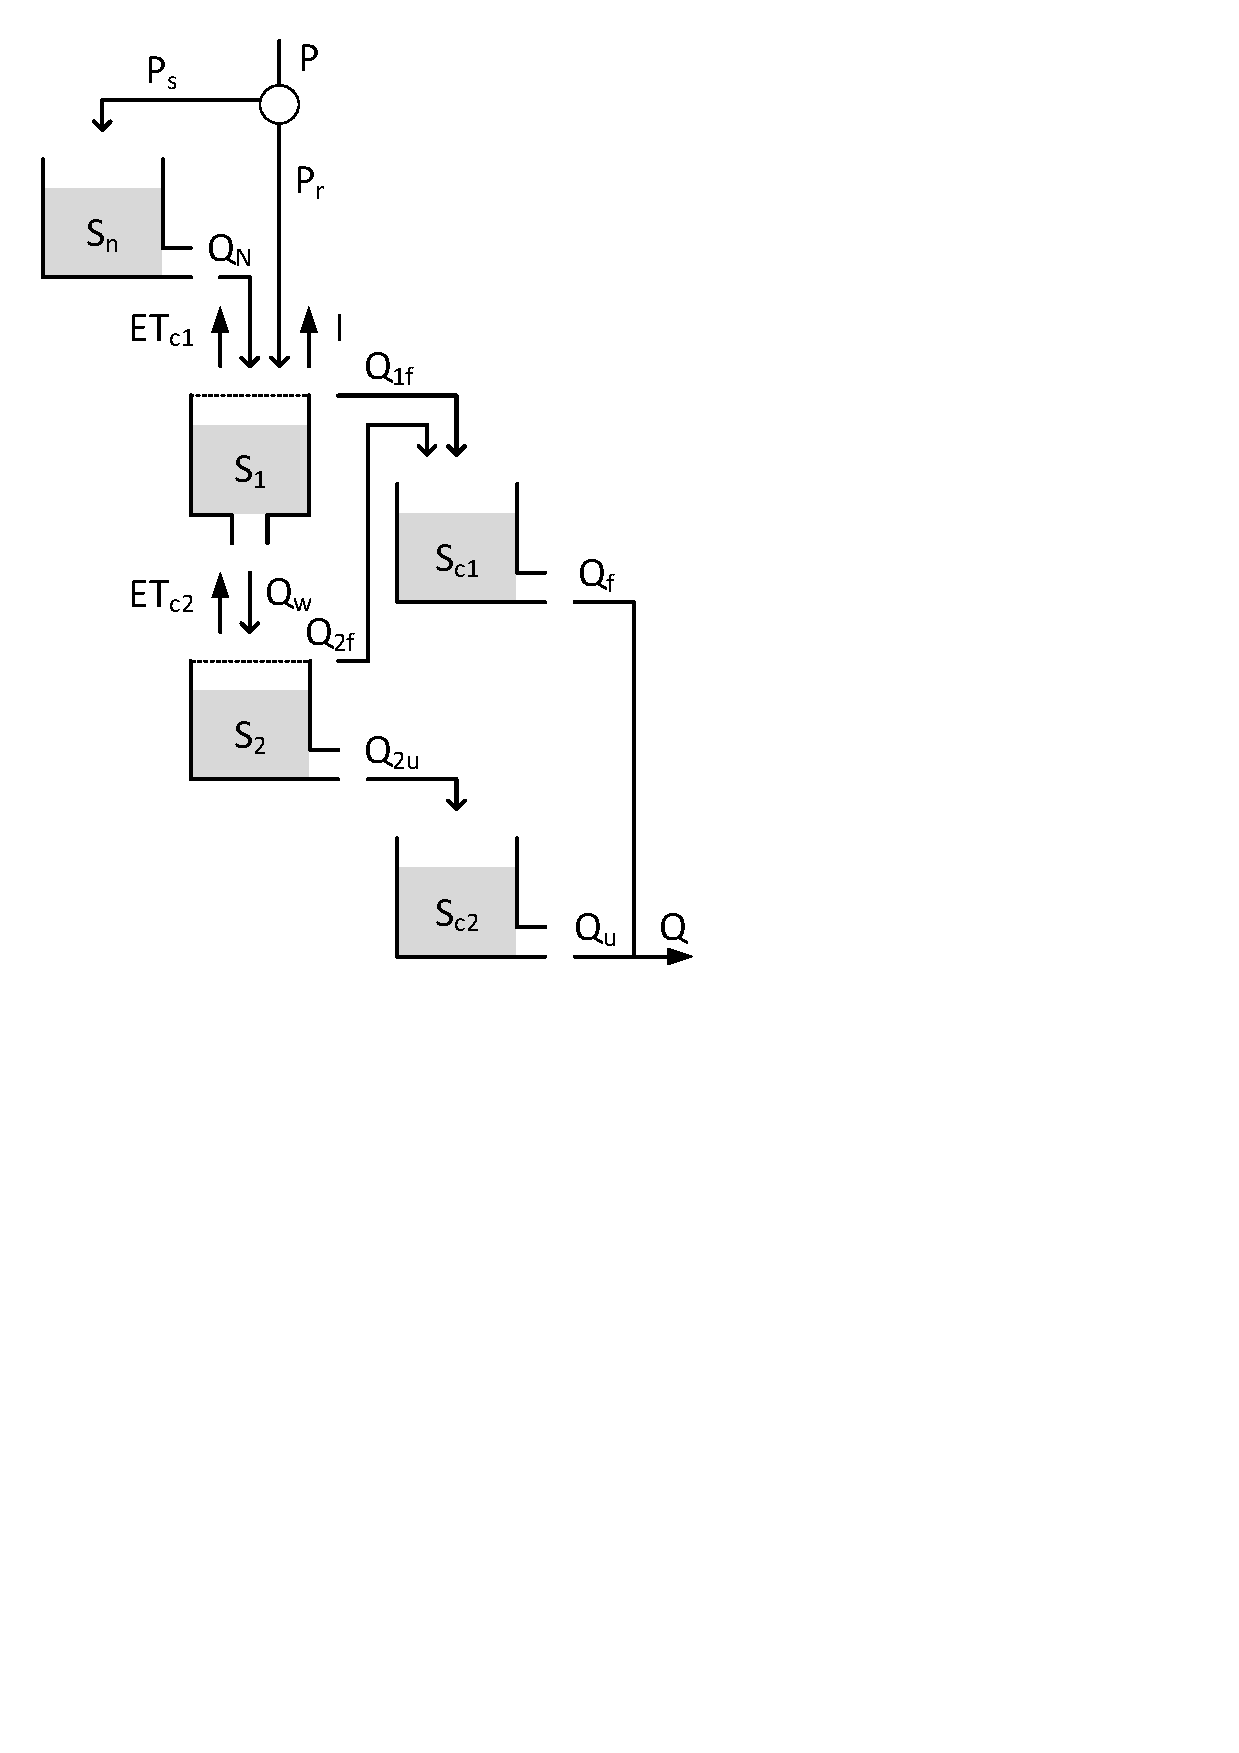
\includegraphics[trim=1cm 13cm 7cm 1cm,width=7cm,keepaspectratio]{./files/35_schematic.pdf}
\caption{Structure of the MOPEX-5 model} \label{fig:35_schematic}
\end{wrapfigure}

\begin{align}
	\frac{dS_n}{dt} &= P_s-Q_{n} \\
	P_s &= \begin{cases}
		P, &\text{if } T \leq T_{crit} \\
		0, & \text{otherwise} \\
	\end{cases} \\
	Q_n &=\begin{cases}
		ddf*(T-T_{crit}), &\text{if } T > T_{crit} \\
		0, & \text{otherwise} \\
	\end{cases}
\end{align}

Where $S_n$ [mm] is the current snow pack. Precipitation occurs as snowfall $P_s$ $[mm/d]$ when current temperature T $[^oC]$ is below threshold $T_{crit}$ $[^oC]$. Snowmelt $Q_N$ $[mm/d]$ occurs when the temperature rises above the threshold temperature and relies in the degree-day factor $dd$ $[mm/^oC/d]$.

} % end of wrapfigure fix
\vspace{5cm}

\begin{align}
	\frac{dS_1}{dt} &= P_r-ET_1-I-Q_{1f}-Q_w \\
	P_r &= \begin{cases}
		P, &\text{if } T > T_{crit} \\
		0, & \text{otherwise} \\
	\end{cases} \\
	ET_{c1} &= \frac{S_1}{S_{b1}}*Ep_c\\
	I &= max\left(0,I_{\alpha} + (1-I_{\alpha})sin\left(2\pi\frac{t+I_{s}}{365/d}\right)\right)\\
	Q_{1f} &= \begin{cases}
		P, &\text{if } S_1 \geq S_{b1} \\
		0, & \text{otherwise} \\
	\end{cases} \\
	Q_w &= t_w*S_1
\end{align}


Where $S_1$ [mm] is the current storage in soil moisture and $P_r$ precipitation as rain $[mm/d]$. Evaporation $ET_1$ $[mm/d]$ depends linearly on current soil moisture, maximum soil moisture $S_{b1}$ [mm] and phenology-corrected potential evapotranspiration: 

\begin{align}
	Ep_c &= Ep*GSI \\
	GSI &= \begin{cases}
		0 , &\text{if } T < T_{min} \\
		\frac{T-T_{min}}{T_{max}-T_{min}}, &\text{if } T_{min} \geq T < T_{max} \\
		1, &\text{if } T \geq T_{max} \\
	\end{cases}
\end{align}

Where GSI is a growing season index based on parameters $T_{min}$ $[^oC]$ and $T_{max}$ $[^oC]$. Interception $I$ $[mm/d]$ depends on the mean intercepted fraction $I_{\alpha}$ [-] and the maximum Leaf Area Index timing $I_{s}$ [d]. Saturation excess flow $Q_{1f}$  $[mm/d]$ occurs when the soil moisture bucket exceeds its maximum capacity. Infiltration to deeper groundwater $Q_w$  $[mm/d]$ depends on current soil moisture and time parameter $t_w$  $[d^{-1}]$.

\begin{align}
	\frac{dS_2}{dt} &= Q_w-ET_2-Q_{2u} - Q_{2f}\\
	ET_{c2} &= \frac{S_2}{S_{e}}*Ep_c\\
	Q_{2u} &= t_u*S_2\\
	Q_{2f} &= \begin{cases}
		Q_w, &\text{if } S_2 \geq S_{b2} \\
		0, & \text{otherwise} \\
	\end{cases}
\end{align}

Where $S_2$ [mm] is the current groundwater storage, refilled by infiltration from $S_1$. Evaporation $ET_2$ $[mm/d]$ depends linearly on current groundwater and root zone storage capacity $S_e$ [mm]. Leakage to the slow runoff store $Q_{2u}$ $[mm/d]$ depends on current groundwater level and time parameter $t_u$ $[d^{-1}]$. When the store reaches maximum capacity $S_{b2}$ [mm], excess flow $Q_{2f}$ $[mm/d]$ is routed towards the fast response routing store.

\begin{align}
	\frac{dS_{c1}}{dt} &= Q_{1f}+Q_{2f}-Q_{f}\\
	Q_f &= t_c*S_{c1}
\end{align}

Where $S_{c1}$ [mm] is current storage in the fast flow routing reservoir, refilled by $Q_{1f}$ and $Q_{2f}$. Routed flow $Q_f$ depends on the mean residence time parameter $t_c$ $[d^{-1}]$.

\begin{align}
	\frac{dS_{c2}}{dt} &= Q_{2u}-Q_{u}\\
	Q_u &= t_c*S_{c2}
\end{align}

Where $S_{c2}$ [mm] is current storage in the slow flow routing reservoir, refilled by $Q_{2u}$. Routed flow $Q_u$ depends on the mean residence time parameter $t_c$ $[d^{-1}]$. Total simulated flow $Q_t$ $[mm/d]$:

\begin{align}
	Q_t &= Q_f + Q_u
\end{align}


\subsubsection{Parameter overview}
% Table generated by Excel2LaTeX from sheet 'Sheet1'
\begin{table}[htbp]
  \centering
    \begin{tabular}{lll}
    \toprule
    Parameter & Unit  & Description \\
    \midrule
    $T_{crit}$ & $^oC$ & Threshold temperature for snowfall and melt \\
    $ddf$ & $mm~^oC^{-1}~d^{-1}$ & Degree-day factor \\
    $S_{b1}$ & $mm$  & Maximum soil moisture storage \\
    $t_w$ & $d^{-1}$ & Runoff coefficient \\
    $I_{\alpha}$ & $-$   & Mean intercepted fraction of precipitation \\
    $I_{s}$ & $d$   & Timing of peak interception capacity \\
    $T_{min}$ & $^oC$ & Minimum temperature to start growing season \\
    $T_{max}$ & $^oC$ & Temperature of maximum plant growth \\
    $S_{b2}$ & $mm$  & Maximum deep storage \\
    $t_u$ & $d^{-1}$ & Runoff coefficient \\
    $S_e$ & $mm$  & Maximum groundwater storage capacity \\
    $t_c$ & $d^{-1}$ & Runoff coefficient \\
    \bottomrule
    \end{tabular}%
  \label{tab:addlabel}%
\end{table}%


\section{MODHYDROLOG (model ID: 36)}
The MODHYDROLOG model (fig.~\ref{fig:36_schematic}) is an elaborate groundwater recharge model, originally created for use in Australia \citep{Chiew1990,Chiew1994}. It has 5 stores (I, D, SMS, GW and CH) and 15 parameters (INSC, COEFF, SQ, SMSC, SUB, CRAK, EM, DSC, ADS, MD, VCOND, DLEV, $k_1$, $k_2$ and $k_3$). It originally includes a routing scheme that allows linking sub-basins together, which has been removed here. The model aims to represent:

\begin{itemizecompact}
\item Interception by vegetation;
\item Infiltration and infiltration excess flow;
\item Depression storage and delayed infiltration;
\item Preferential groundwater recharge, interflow and saturation excess flow;
\item Groundwater recharge resulting from filling up of soil moisture storage capacity;
\item Water exchange between shallow and deep aquifers;
\item Water exchange between aquifer and river channel.
\end{itemizecompact}

\subsection{MARRMoT model name}
m\_36\_modhydrolog\_15p\_5s \\

% Equations
\subsection{Model equations}

% Model layout figure
{ 																	% This ensures it doesn't warp text further down
\begin{wrapfigure}{l}{7cm}
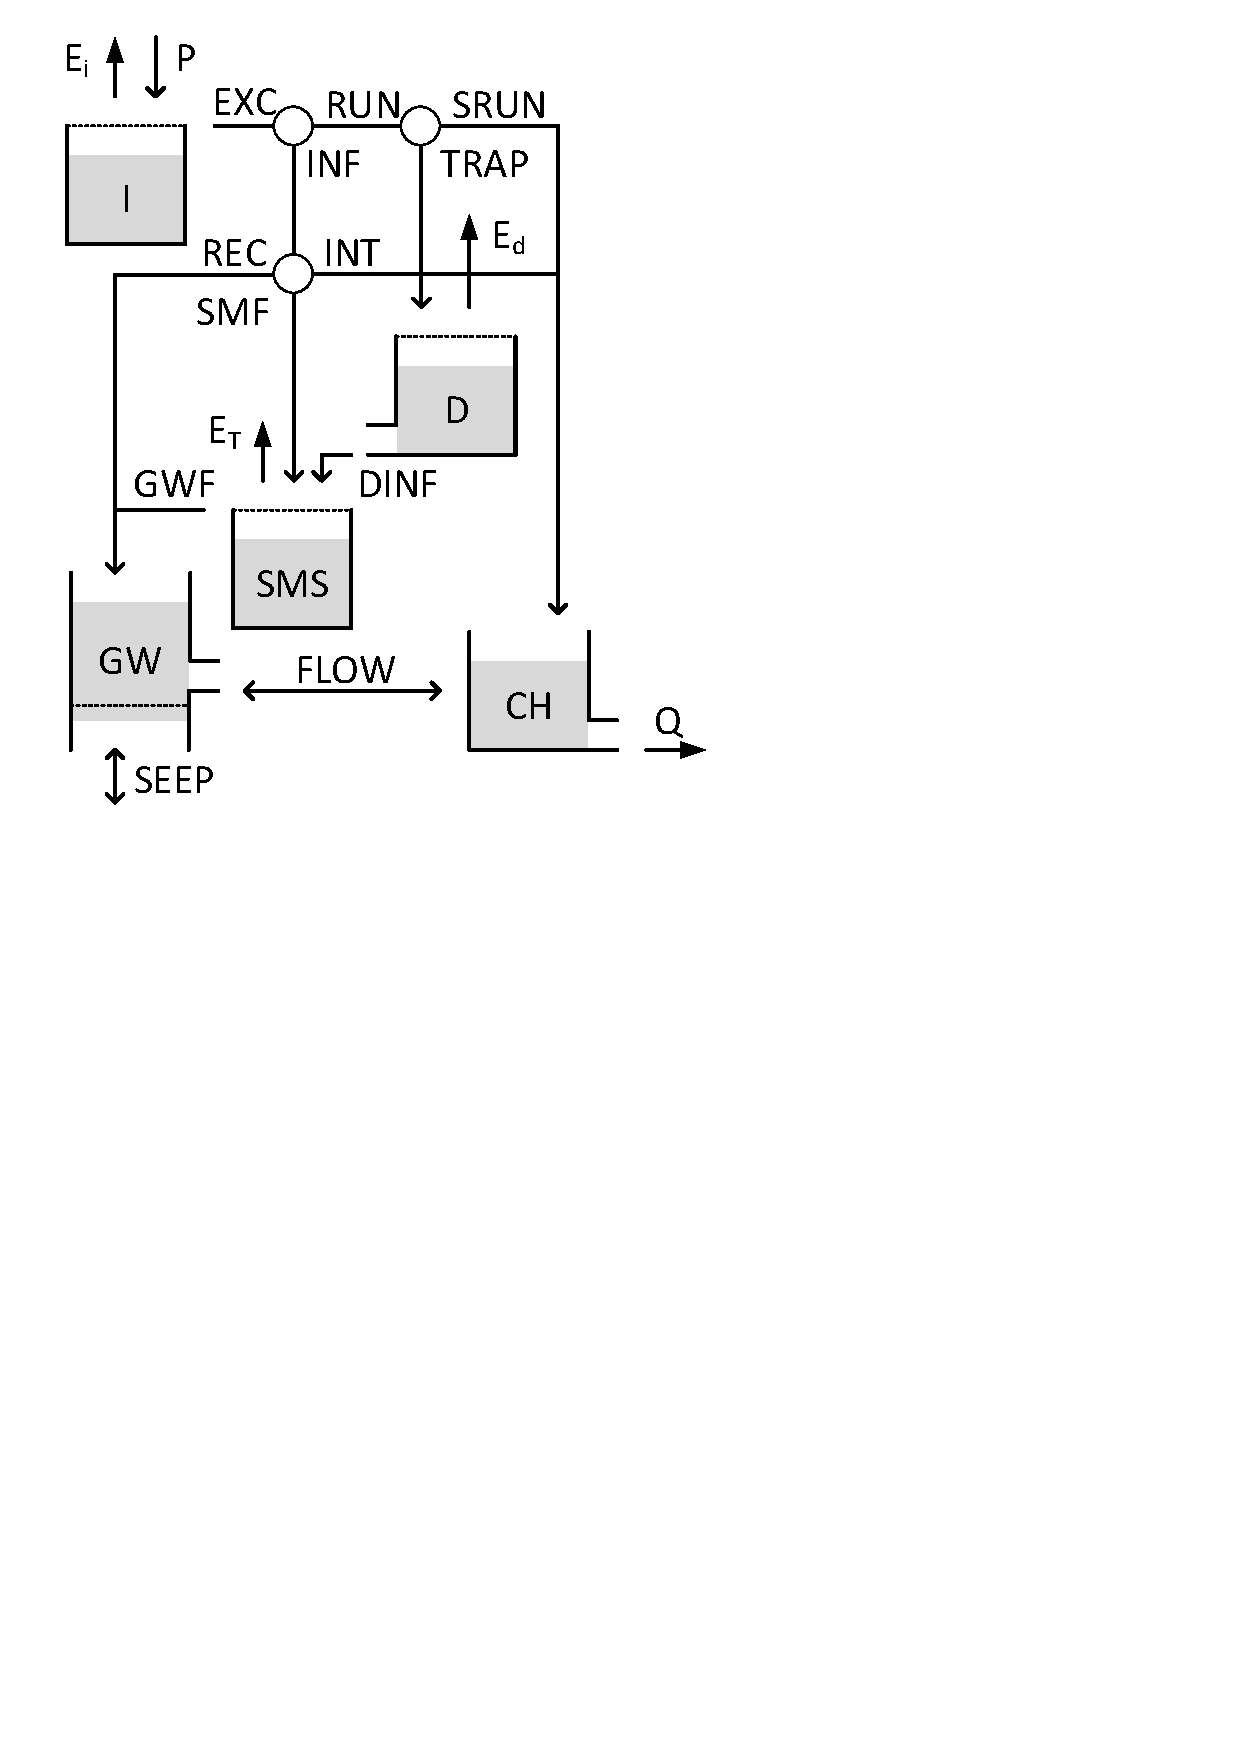
\includegraphics[trim=1cm 16.5cm 9cm 1cm,width=7cm,keepaspectratio]{./AppA_files/36_schematic.pdf}
\caption{Structure of the MODHYDROLOG model} \label{fig:36_schematic}
\end{wrapfigure}

\begin{align}
	\frac{dI}{dt} &= P-E_i-EXC \\
	E_i &= \begin{cases}
		E_p, &\text{if } I > 0 \\
		0, & \text{otherwise} \\
	\end{cases} \\
	EXC &= 
	\begin{cases}
		P, & \text{if } I = INSC \\
		0, & \text{otherwise}
	\end{cases}
\end{align}

Where I [mm] is the current interception storage, $P$ the rainfall [mm/d], $E_i$ the evaporation from the interception store [mm/d] and $EXC$ the excess rainfall [mm/d]). Evaporation is assumed to occur at the potential rate $E_p$ [mm/d] when possible. When I exceeds the maximum interception capacity $INSC$ [mm], water is routed to the rest of the model as excess precipitation $EXC$. The soil moisture store SMS is instrumental in dividing runoff between infiltration and surface flow:

} % end of wrapfigure fix

\vspace{1cm}
\begin{align}
	\frac{dSMS}{dt} &= SMF+DINF-E_T-GWF\\
	SMF &= INF-INT-REC\\
		&INF = min\left(COEFF * exp\left(\frac{-SQ*SMS}{SMSC}\right),EXC\right)\\
		&INT = SUB*\frac{SMS}{SMSC} * INF \\
		&REC = CRAK*\frac{SMS}{SMSC}*(INF-INT)\\	
	E_T &=min\left(EM*\frac{SMS}{SMSC},PET\right)\\
	GWF &= \begin{cases}
		SMF, &\text{if } SMS = SMSC\\
		0, &\text{otherwise}
	\end{cases}
\end{align}

Where SMS is the current storage in the soil moisture store [mm]. SMF [mm/d] and DINF [mm/d] are the infiltration and delayed infiltration respectively. INF is total infiltration [mm/d] from excess precipitation, based on maximum infiltration loss parameter COEFF [-], the infiltration loss exponent SQ [-] and the ratio between current soil moisture storage SMS [mm] and the maximum soil moisture capacity SMSC [mm]. INT represents interflow and saturation excess flow [mm/d], using a constant of proportionality SUB [-]. REC is preferential recharge of groundwater [mm/d] based on another constant of proportionality CRAK [-]. SMF is flow into soil moisture storage [mm/d]. $E_T$ evaporation from the soil moisture that occurs at the potential rate when possible [mm/d], based on the maximum plant-controlled rate EM [mm/d]. GWF is the flow to the groundwater store [mm/d]:

\begin{align}
	\frac{dD}{dt} &= TRAP - E_D - DINF \\
	TRAP &= ADS*exp\left(-MD\frac{D}{DSC-D}\right)*RUN\\
		&RUN = EXC-INF\\
	E_D &= \begin{cases}
			ADS*E_p, &\text{if } D > 0 \\
			0, &\text{otherwise} \\
		\end{cases}\\
	DINF &= \begin{cases}
			ADS*RATE, &\text{if }  D > 0\\
			0, &\text{otherwise} \\
		\end{cases} \\
		&RATE = COEFF*exp\left(-SQ\frac{SMS}{SMSC}\right) - INF-INT-REC
\end{align}

Where TRAP [mm/d] is the part of overland flow captured in the depression store (equation taken from \citet{Porter1971}), $E_D$ the evaporation from the depression store [mm/d], and DINF delayed infiltration to soil moisture [mm/d]. TRAP uses DSC as the maximum depression store capacity [mm], ADS as the fraction of land functioning as depression storage [-] and MD a depression storage parameter [-]. $E_D$ relies on the potential evapotranspiration $E_p$. The groundwater store has no defined upper and lower boundary and instead fluctuates around a datum DLEV [mm]:

\begin{align}
	\frac{dGW}{dt} &= REC+GWF - SEEP - FLOW\\
	SEEP &= VCOND*\left(GW - DLEV\right) \\
	FLOW &= \begin{cases}
			k_1*|GW|+k_2*\left(1-exp(-k_3*|GW|)\right), &\text{if } GW \geq 0\\
			-\left(k_1*|GW|+k_2*\left(1-exp(-k_3*|GW|)\right)\right), &\text{if } GW < 0\\
		\end{cases}
\end{align}

Where SEEP [mm/d] is the exchange with a deeper aquifer (can be negative or positive) and FLOW [mm/d] the exchange with the channel (can be negative or positive). VCOND $[d^{-1}]$ is a leakage coefficient, DLEV a datum around which the groundwater level can fluctuate, and $k_1$, $k_2$ and $k_3$ are runoff coefficients. The channel store aggregates incoming fluxes and produces the total runoff $Q_t$ [mm/d]:

\begin{align}
	\frac{dCH}{dt} &= SRUN + INT + FLOW - Q \\
	SRUN &= RUN-TRAP \\
	Q_t &= \begin{cases}
		CH, &\text{if } CH > 0\\
		0, &\text{otherwise}
	\end{cases}
\end{align}

\newpage
\subsection{Parameter overview}
% Table generated by Excel2LaTeX from sheet 'Sheet1'
\begin{table}[htbp]
  \centering
    \begin{tabular}{lll}
    \toprule
    Parameter & Unit  & Description \\
    \midrule
    INSC  & $mm$  & Maximum interception capacity \\
    COEFF & $mm~d^{-1}$ & Maximum infiltration loss \\
    SQ    & $-$   & Infiltration loss exponent \\
    SMSC  & $mm$  & Maximum soil moisture storage \\
    SUB   & $-$   & Proportionality constant \\
    CRAK  & $-$   & Proportionality constant \\
    EM    & $mm~d^{-1}$ & Maximum plant-controlled evaporation rate \\
    DSC   & $mm$  & Maximum depression storage \\
    ADS   & $-$   & Fraction of area functioning as depression store \\
    MD    & $-$   & Depression store shape parameter \\
    VCOND & $d^{-1}$ & Runoff coefficient \\
    DLEV  & $mm$  & Datum of groundwater store \\
    $k_1$ & $d^{-1}$ & Runoff coefficient \\
    $k_2$ & $d^{-1}$ & Runoff coefficient \\
    $k_3$ & $d^{-1}$ & Runoff coefficient \\
    \bottomrule
    \end{tabular}%
  \label{tab:addlabel}%
\end{table}%

\subsection{HBV-96 (model ID: 37)}
The HBV-96 model (fig.~\ref{fig:37_schematic}) was originally developed for use in Sweden, but has been widely applied beyond its original region \citep{Lindstrom1997}. It can account for different land types (forest, open ground, lakes) but that distinction has been removed here. Correction factors for climate inputs have also been removed. It has 5 stores and 15 parameters ($TT$, $TTI$, $CFR$, $CFMAX$, $TTM$, $WHC$, $CFLUX$, $FC$, $LP$, $\beta$, $K_0$, $\alpha$, $c$, $K_1$ and $MAXBAS$) parameters. The model aims to represent:

\begin{itemizecompact}
\item Snow accumulation, melt and refreezing;
\item Infiltration and capillary flow to, and evaporation from, soil moisture;
\item A non-linear storage-runoff relationship from the upper runoff-generating zone;
\item A linear storage-runoff relationship from the lower runoff-generating zone.
\end{itemizecompact}

\subsubsection{File names}
\begin{tabular}{@{}ll}
Model: &m\_37\_hbv\_15p\_5s \\
Parameter ranges: &m\_37\_hbv\_15p\_5s\_parameter\_ ranges \\
\end{tabular}

% Equations
\subsubsection{Model equations}

% Model layout figure
{ 																	% This ensures it doesn't warp text further down
\begin{wrapfigure}{l}{5cm}
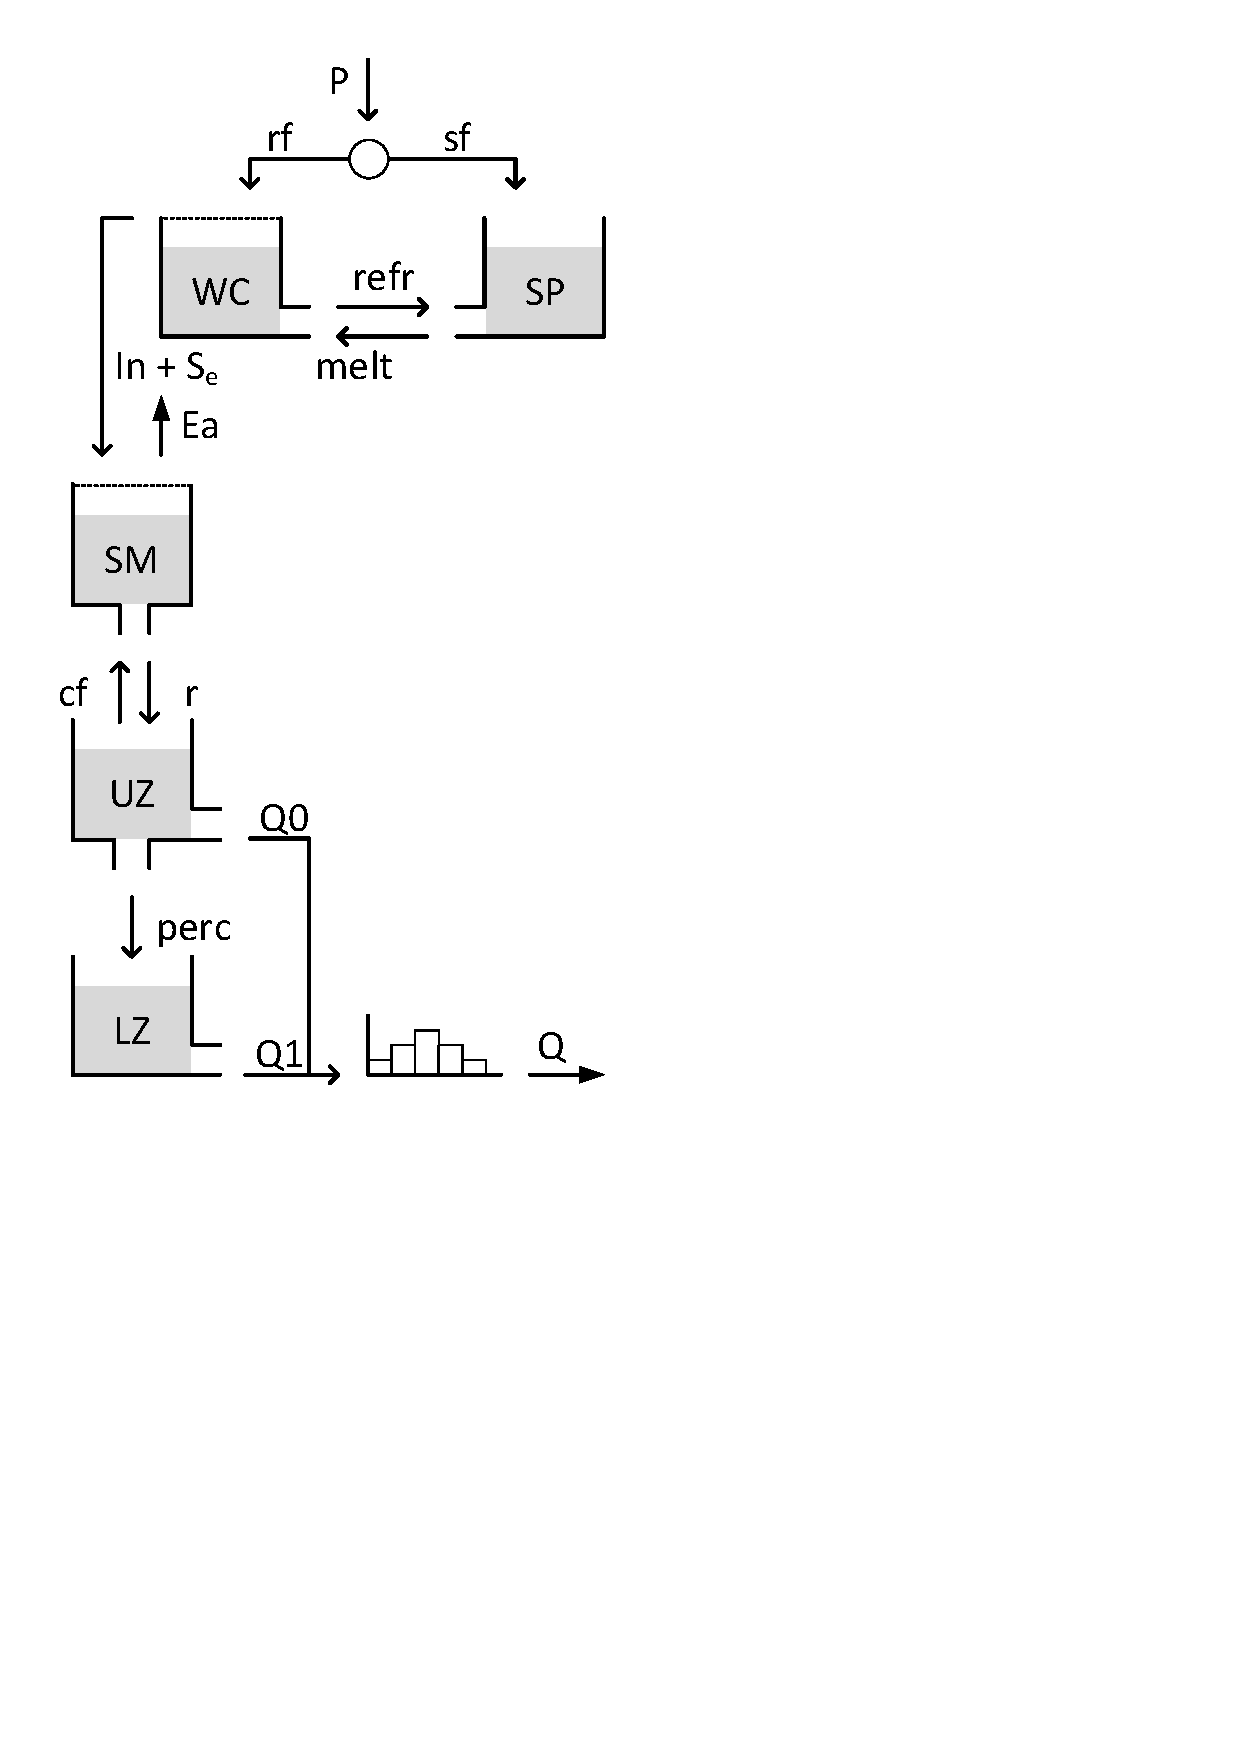
\includegraphics[trim=1cm 11.1cm 7cm 1cm,width=7cm,keepaspectratio]{./files/37_schematic.pdf}
\caption{Structure of the HBV-96 model} \label{fig:37_schematic}
\end{wrapfigure}

\begin{align}
	\frac{dSP}{dt} &= sf+refr-melt \\
	sf &= \begin{cases}
		P, &\text{if } T \leq TT-\frac{1}{2}TTI \\
		P*\frac{ TT+\frac{1}{2}TTI-T}{TTI}, &\text{otherwise}\\
		0, &\text{if } T \geq TT+\frac{1}{2}TTI \\
	\end{cases} \\
	refr &= 
	\begin{cases}
		CFR*CFMAX*(TTM-T), & \text{if } T < TTM \\
		0, & \text{otherwise}\\
	\end{cases}\\
	melt &= \begin{cases}
		CFMAX*(T-TTM), &\text{if } T \geq TTM\\
		0, &\text{otherwise}
	\end{cases}
\end{align}

Where SP is the current snow storage [mm]. $sf$ is precipitation that occurs as snowfall [mm/d] based on daily precipitation P [mm/d], threshold temperature for snowfall TT [\degree C] and the snowfall threshold interval length TTI [\degree C]. $refr$ [mm/d] is the refreezing of liquid snow if the current temperature T is below the melting threshold TTM [\degree C], using a coefficient of refreezing CFR [-] and a degree-day factor CFMAX [mm/d/\degree C]. $melt$ represents snowmelt if the current temperature T is below the melting threshold TTM, using the degree-day factor CFMAX. 

} % end of wrapfigure fix

\begin{align}
	\frac{dWC}{dt} &= rf+melt-refr-in-S_{excess}\\
	rf &= \begin{cases}
		0, &\text{if } T \leq TT-\frac{1}{2}TTI \\
		P*\frac{T- TT+\frac{1}{2}TTI}{TTI}, &\text{otherwise}\\
		P, &\text{if } T \geq TT+\frac{1}{2}TTI \\
	\end{cases} \\
	in &= \begin{cases}
		rf+melt, &\text{if } WC \geq WHC*SP\\
		0, &\text{otherwise}\\
	\end{cases}\\
	S_{e} &= \begin{cases}
		WC-WHC*SP, &\text{if } WC \geq WHC*SP\\
		0, &\text{otherwise}\\
	\end{cases}		
\end{align}

Where WC is the current liquid water content in the snow pack [mm], $rf$ is the precipitation occurring as rain [mm/d] based on temperature threshold parameters TT and TTI, $refr$ is the refreezing flux, and $in$ the infiltration to soil moisture [mm/d] that occurs when the water holding capacity of snow gets exceeded. $S_{excess}$ [mm/d] represents excess stored water that is freed when the total possible storage of liquid water in the snow pack is reduced.

\begin{align}
	\frac{dSM}{dt} &= (in+S_{excess})+cf-E_a-r\\
	cf &= CFLUX*\left(1-\frac{SM}{FC}\right)\\
	E_a &= \begin{cases}
		E_p, &\text{if } SM \geq LP*FC\\
		E_p*\frac{SM}{LP*FC}, &\text{otherwise}\\
	\end{cases}\\
	r &= (in+S_{excess})*\left(\frac{SM}{FC}\right)^\beta
\end{align}
  
Where SM is the current storage in soil moisture [mm], $in$ the infiltration from the surface, $cf$ the capillary rise [mm/d] from the unsaturated zone, $E_a$ evaporation [mm/d] and $r$ the flow to the upper zone [mm/d]. Capillary rise depends on the maximum rate CFLUX [mm/d], scaled by the available storage in soil moisture, expressed as the ration between current storage SM and maximum storage FC [mm]. Evaporation $E_a$ occurs at the potential rate $E_p$ when current soil moisture is above the wilting point LP [mm], and is scaled linearly below that. Runoff $r$ to the upper zone has a potentially non-linear relationship with infiltration in through parameter $\beta$ [-].

\begin{align}
	\frac{dUZ}{dt} &= r-cf-Q_0-perc \\
	Q_0 &= K_0*UZ^{(1+\alpha)}\\
	perc &= c.
\end{align}

Where UZ is the current storage [mm] in the upper zone. Outflow $Q_0$ [mm/d] from the reservoir has a non-linear relation with storage through time scale parameter $K_0$ [$d^{-1}$] and and $\alpha$ [-]. Percolation $perc$ [mm/d] to the lower zone is given as a constant rate $c$ [mm/d]S.

\begin{align}
	\frac{dLZ}{dt} &= perc-Q_1 \\
	Q_1 &= K_1*LZ
\end{align}

Where LZ is the current storage [mm] in the lower zone. Outflow $Q_1$ [mm/d] from the reservoir has a linear relation with storage through time scale parameter $K_1$ [$d^{-1}$]. Total outflow is generated by summing $Q_0$ and $Q_1$ and applying a triangular transform based on lag parameter MAXBAS [d].

\subsubsection{Parameter overview}
% Table generated by Excel2LaTeX from sheet 'Sheet1'
\begin{table}[htbp]
  \centering
    \begin{tabular}{lll}
    \toprule
    Parameter & Unit  & Description \\
    \midrule
    $TT$  & $^oC$ & Threshold temperature for snowfall \\
    $TTI$ & $^oC$ & Threshold temperature interval length \\
    $CFR$ & $-$   & Refreezing coefficient \\
    $CFMAX$ & $mm~^oC^{-1}~d^{-1}$ & Degree-day factor \\
    $TTM$ & $^oC$ & Threshold temperature for snowmelt \\
    $WHC$ & $-$   & Water holding capacity as fraction of current snow pack \\
    $CFLUX$ & $mm~d^{-1}$ & Maximum capillary rise rate \\
    $FC$  & $mm$  & Field capacity \\
    $LP$  & $-$   & Wilting point as fraction of $FC$ \\
    $\beta$ & $-$   & Recharge non-linearity \\
    $K_0$ & $d^{-1}$ & Runoff coefficient \\
    $\alpha$ & $-$   & Runoff non-linearity \\
    $c$   & $mm~d^{-1}$ & Percolation rate \\
    $K_1$ & $d^{-1}$ & Runoff coefficient \\
    $MAXBAS$ & $d$   & Unit Hydrograph time base \\
    \bottomrule
    \end{tabular}%
  \label{tab:addlabel}%
\end{table}%


\section{Tank Model - SMA (model ID: 38)}
The Tank Model (fig.~\ref{fig:38_schematic}) is originally developed for use in constantly saturated soils in Japan \citep{Sugawara1979}. This alternative Tank model - SMA (soil moisture accounting) version was developed for regions that are not continuously saturated \citep{Sugawara1995}. This model is identical to the original tank model, but has an increased depth in the first store to represent primary soil moisture, and adds a new store to represent secondary soil moisture. It has 5 stores and 16 parameters ($sm_1$, $sm_2$, $k_1$, $k_2$, $A_0$, $A_1$, $A_2$, $t_1$, $t_2$, $B_0$, $B_1$, $t_3$, $C_0$, $C_1$, $t_4$ and $D_1$). The model aims to represent:

\begin{itemizecompact}
\item Runoff on increasing time scales with depth;
\item Soil moisture storage;
\item capillary rise to replenish soil moisture.
\end{itemizecompact}

\subsection{MARRMoT model name}
m\_38\_tank2\_16p\_5s \\

% Equations
\subsection{Model equations}

% Model layout figure
{ 																	% This ensures it doesn't warp text further down
\begin{wrapfigure}{l}{6cm}
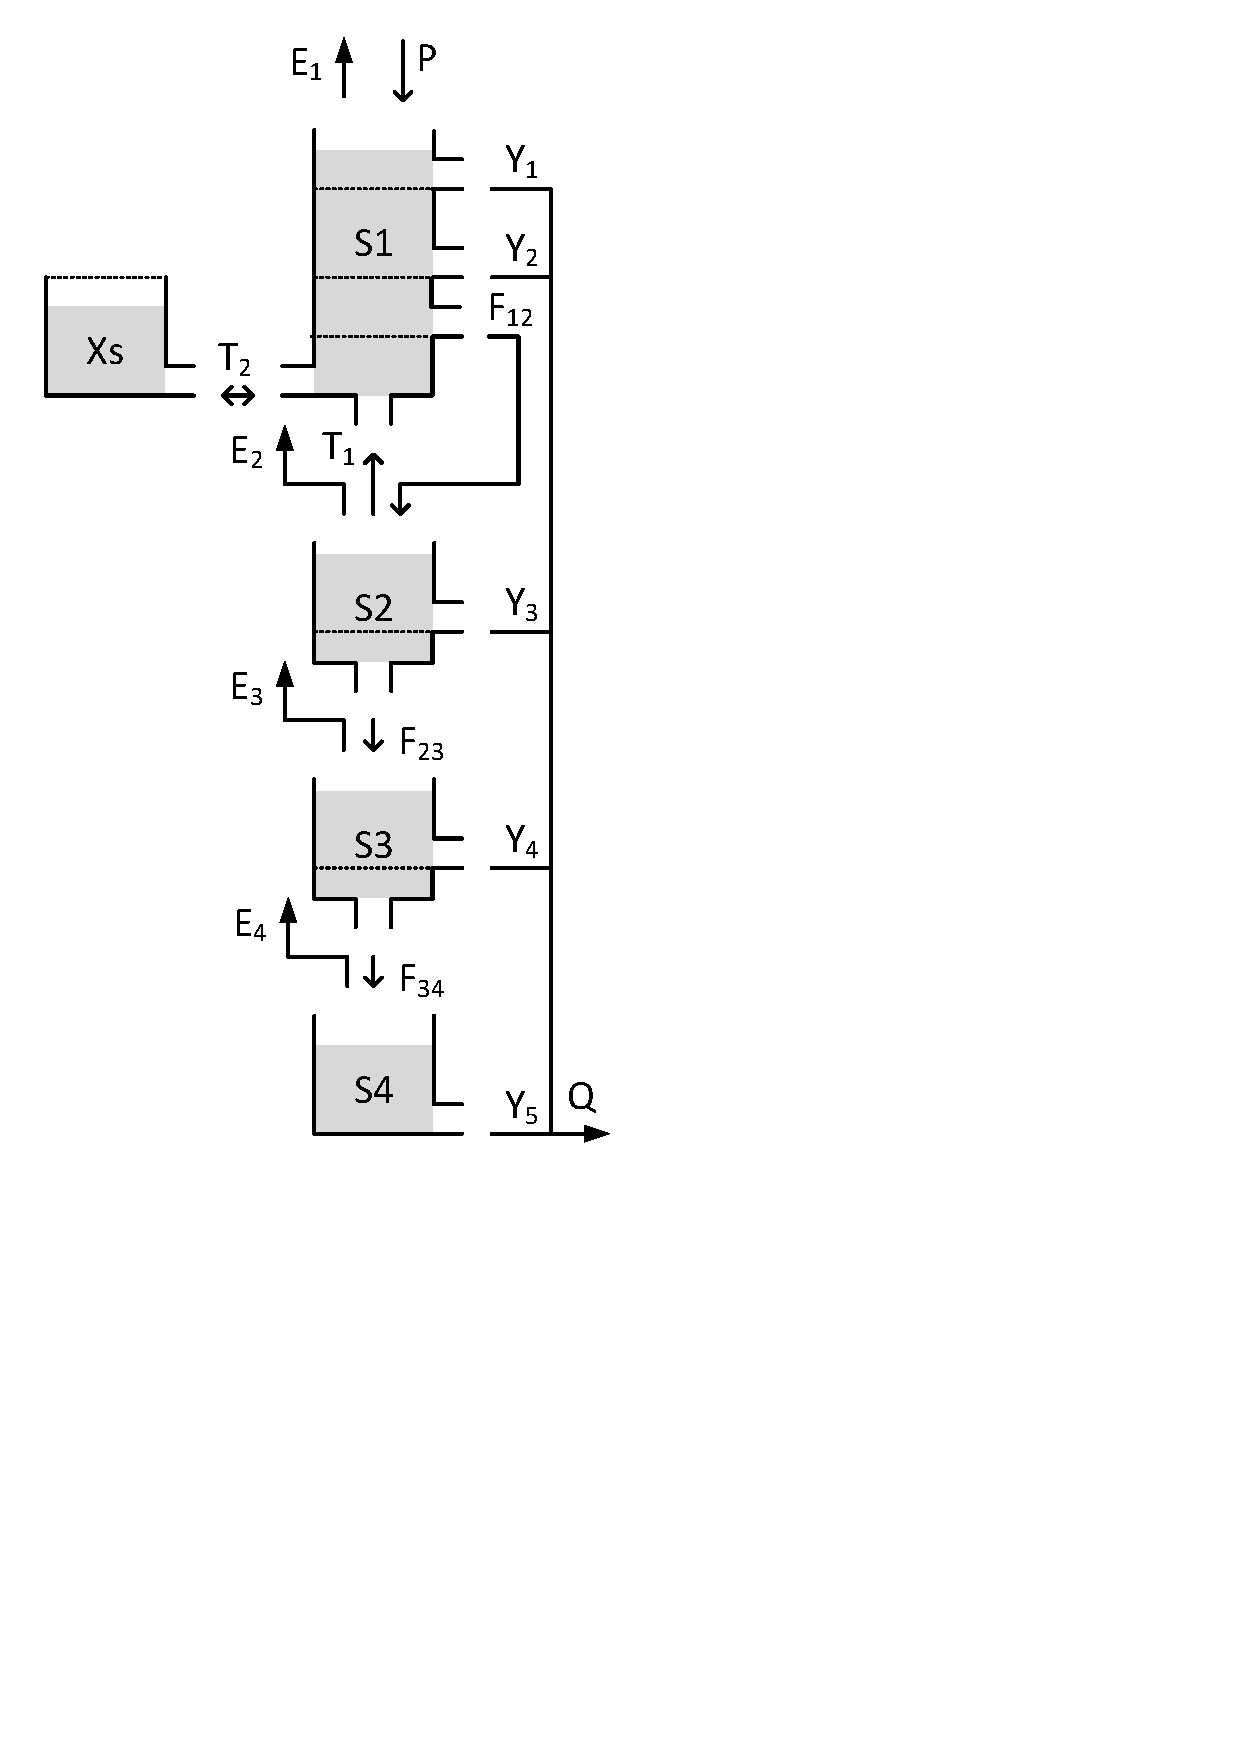
\includegraphics[trim=1cm 10cm 7cm 1cm,width=7cm,keepaspectratio]{./AppA_files/38_schematic.pdf}
\caption{Structure of the Tank Model - SMA} \label{fig:38_schematic}
\end{wrapfigure}

\begin{align}
	\frac{dS_1}{dt} &= P+T_1-T_2-E_1-F_{12}-Y_2-Y_1 \\
	T_1 &= k_1\left(1-\frac{S_1}{sm_1}\right), \text{if } S_1 < sm_1\\
	T_2 &= k_2\left(\frac{min(S_1,sm_1)}{sm_1}-\frac{X_s}{sm_2}\right) \\
	E_1 &= \begin{cases}
		Ep, &\text{if } S_1 > 0 \\
		0, & \text{otherwise} \\
	\end{cases} \\
	F_{12} &= \begin{cases}
		A_0*(S_1-sm_1), & \text{if } S_1 > sm_1 \\
		0, & \text{otherwise}
	\end{cases}\\
	Y_2 &= 
	\begin{cases}
		A_2*(S_1-t_2), & \text{if } S_1 > t_2 \\
		0, & \text{otherwise}
	\end{cases}\\
	Y_1 &= 
	\begin{cases}
		A_1*(S_1-t_1), & \text{if } S_1 > t_1 \\
		0, & \text{otherwise}\\
	\end{cases}
\end{align}

Where $S_1$ [mm] is the current storage in the upper zone, refilled by precipitation $P$ 

} % end of wrap figure

\noindent$[mm/d]$ and drained by evaporation $E_1$ $[mm/d]$, drainage $F_{12}$ $[mm/d]$ and surface runoff $Y_1$ $[mm/d]$ and $Y_2$ $[mm/d]$. If $S_1$ is below the soil moisture threshold $sm_1$ [mm], capillary rise $T_1$  $[mm/d]$ from store $S_2$ can occur. Capillary rise has a base rate $k_1$  $[mm/d]$ and decreases linearly as soil moisture $S_1$ nears $sm_1$. This store is connected to the secondary soil moisture store $X_s$ through transfer flux $T_2$  $[mm/d]$. This flux can work in either direction, based on a base rate $k_2$ [mm/d], the current storages $S_1$ [mm] and $X_s$ [mm] and the maximum soil moistures storages $sm_1$ [mm] and $sm_2$ [mm]. Evaporation $E_1$ occurs at the potential rate $E_p$ $[mm/d]$ if water is available. Drainage to the intermediate layer has a linear relationship with storage through time scale parameter $A_0$ $[d^{-1}]$. Surface runoff $Y_2$ and $Y_1$ occur when $S_1$ is above thresholds $t_2$ [mm] and $t_1$ [mm] respectively. Both are linear relationships through time parameters $A_2$ $[d^{-1}]$ and $A_1$ $[d^{-1}]$ respectively.

\begin{align}
	\frac{dX_s}{dt} &= T_2
\end{align}

Where $X_s$ [mm] is the current storage in the secondary soil moisture zone. This zone has a maximum capacity $sm_2$ [mm], used in the calculation of $T_2$. $T_2$ can be both positive and negative.

\begin{align}
	\frac{dS_2}{dt} &= F_{12}-E_2-T_1-F_{23}-Y_3\\
	E_2 &= \begin{cases}
		Ep, &\text{if } S_1 = 0 ~\&~ S_2 > 0\\
		0, & \text{otherwise} \\
	\end{cases} \\
	F_{23} &= B_0*S_2\\
	Y_3 &= 
	\begin{cases}
		B_1*(S_2-t_3), & \text{if } S_2 > t_3 \\
		0, & \text{otherwise}
	\end{cases}
\end{align}

Where $S_2$ [mm] is the current storage in the intermediate zone, refilled by drainage $F_{12}$ from the upper zone and drained by evaporation $E_2$ $[mm/d]$, drainage $F_{23}$ $[mm/d]$ and intermediate discharge $Y_3$ $[mm/d]$. $E_2$ occurs at the potential rate $E_p$ if water is available and the upper zone is empty. Drainage to the third layer $F_{23}$ has a linear relationship with storage through time scale parameter $B_0$ $[d^{-1}]$. Intermediate runoff $Y_3$ occurs when $S_2$ is above threshold $t_3$ [mm] and has a linear relationship with storage through time scale parameter $B_1$ $[d^{-1}]$.

\begin{align}
	\frac{dS_3}{dt} &= F_{23}-E_3-F_{34}-Y_4\\
	E_3 &= \begin{cases}
		Ep, &\text{if } S_1 = 0 ~\&~ S_2 = 0 ~\&~ S_3 > 0\\
		0, & \text{otherwise} \\
	\end{cases} \\
	F_{34} &= C_0*S_3\\
	Y_4 &= 
	\begin{cases}
		C_1*(S_3-t_4), & \text{if } S_3 > t_4 \\
		0, & \text{otherwise}
	\end{cases}
\end{align}

Where $S_3$ [mm] is the current storage in the sub-base zone, refilled by drainage $F_{23}$ from the intermediate zone and drained by evaporation $E_3$ $[mm/d]$, drainage $F_{34}$ $[mm/d]$ and sub-base discharge $Y_4$ $[mm/d]$. $E_3$ occurs at the potential rate $E_p$ if water is available and the upper zones are empty. Drainage to the fourth layer $F_{34}$ has a linear relationship with storage through time scale parameter $C_0$ $[d^{-1}]$. Sub-base runoff $Y_4$ occurs when $S_3$ is above threshold $t_4$ [mm] and has a linear relationship with storage through time scale parameter $C_1$ $[d^{-1}]$.

\begin{align}
	\frac{dS_4}{dt} &= F_{34}-E_4-Y_5\\
	E_4 &= \begin{cases}
		Ep, &\text{if } S_1 = 0 ~\&~ S_2 = 0 ~\&~ S_3 = 0 ~\&~ S_4 > 0\\
		0, & \text{otherwise} \\
	\end{cases} \\
	Y_5 &= D_1*S_4
\end{align}

Where $S_4$ [mm] is the current storage in the base layer, refilled by drainage $F_{34}$ from the sub-base zone and drained by evaporation $E_4$ $[mm/d]$ and baseflow $Y_5$ $[mm/d]$. $E_4$ occurs at the potential rate $E_p$ if water is available and the upper zones are empty. Baseflow $Y_5$ has a linear relationship with storage through time scale parameter $D_1$ $[d^{-1}]$. Total runoff:

\begin{align}
	Q_t &= Y_1+Y_2+Y_3+Y_4+Y_5
\end{align}

\newpage
\subsection{Parameter overview}
% Table generated by Excel2LaTeX from sheet 'Sheet1'
\begin{table}[htbp]
  \centering
    \begin{tabular}{lll}
    \toprule
    Parameter & Unit  & Description \\
    \midrule
    $sm_1$ & $mm$  & Soil moisture threshold for capillary rise \\
    $sm_2$ & $mm$  & Maximum soil mositure storage \\
    $k_1$ & $mm~d^{-1}$ & Base capillary rise rate \\
    $k_2$ & $mm~d^{-1}$ & Base soil moisture exchange rate \\
    $A_0$ & $d^{-1}$ & Runoff coefficient \\
    $A_1$ & $d^{-1}$ & Runoff coefficient \\
    $A_2$ & $d^{-1}$ & Runoff coefficient \\
    $t_1$ & $mm$  & Threshold for runoff generation \\
    $t_2$ & $mm$  & Threshold for runoff generation \\
    $B_0$ & $d^{-1}$ & Runoff coefficient \\
    $B_1$ & $d^{-1}$ & Runoff coefficient \\
    $t_3$ & $mm$  & Threshold for runoff generation \\
    $C_0$ & $d^{-1}$ & Runoff coefficient \\
    $C_1$ & $d^{-1}$ & Runoff coefficient \\
    $t_4$ & $mm$  & Threshold for runoff generation \\
    $D_1$ & $d^{-1}$ & Runoff coefficient \\
    \bottomrule
    \end{tabular}%
  \label{tab:addlabel}%
\end{table}%

\section{Midlands Catchment Runoff  Model (model ID: 39)}
The Midlands Catchment Runoff model (fig.~\ref{fig:39_schematic}) is intended to be used in a flood-forecasting setting \citep{Moore2001}. To reduce the number of free parameters, the original evaporation routines and routing are somewhat simplified here. The model has 5 stores and 16 parameters ($S_{max}$, $c_{max}$, $c_0$, $c_1$, $c_e$, $D_{surp}$, $k_d$, $\gamma_d$, $q_{p,max}$, $k_g$, $\tau$, $S_{bf}$, $k_{cr}$, $\gamma_{cr}$, $k_{or}$ and $\gamma_{or}$). The model aims to represent:

\begin{itemizecompact}
\item Interception by vegetation;
\item Direct runoff from a variable contributing area;
\item A deficit-based approach to soil moisture accounting and interflow and percolation;
\item Baseflow from groundwater;
\item Uniform flood flood wave distribution in time;
\item In-channel and out-of-channel flood routing.
\end{itemizecompact}

\subsection{MARRMoT model name}
m\_39\_mcrm\_16p\_5s \\

% Equations
\subsection{Model equations}

% Model layout figure
{ 																	% This ensures it doesn't warp text further down
\begin{wrapfigure}{l}{5cm}
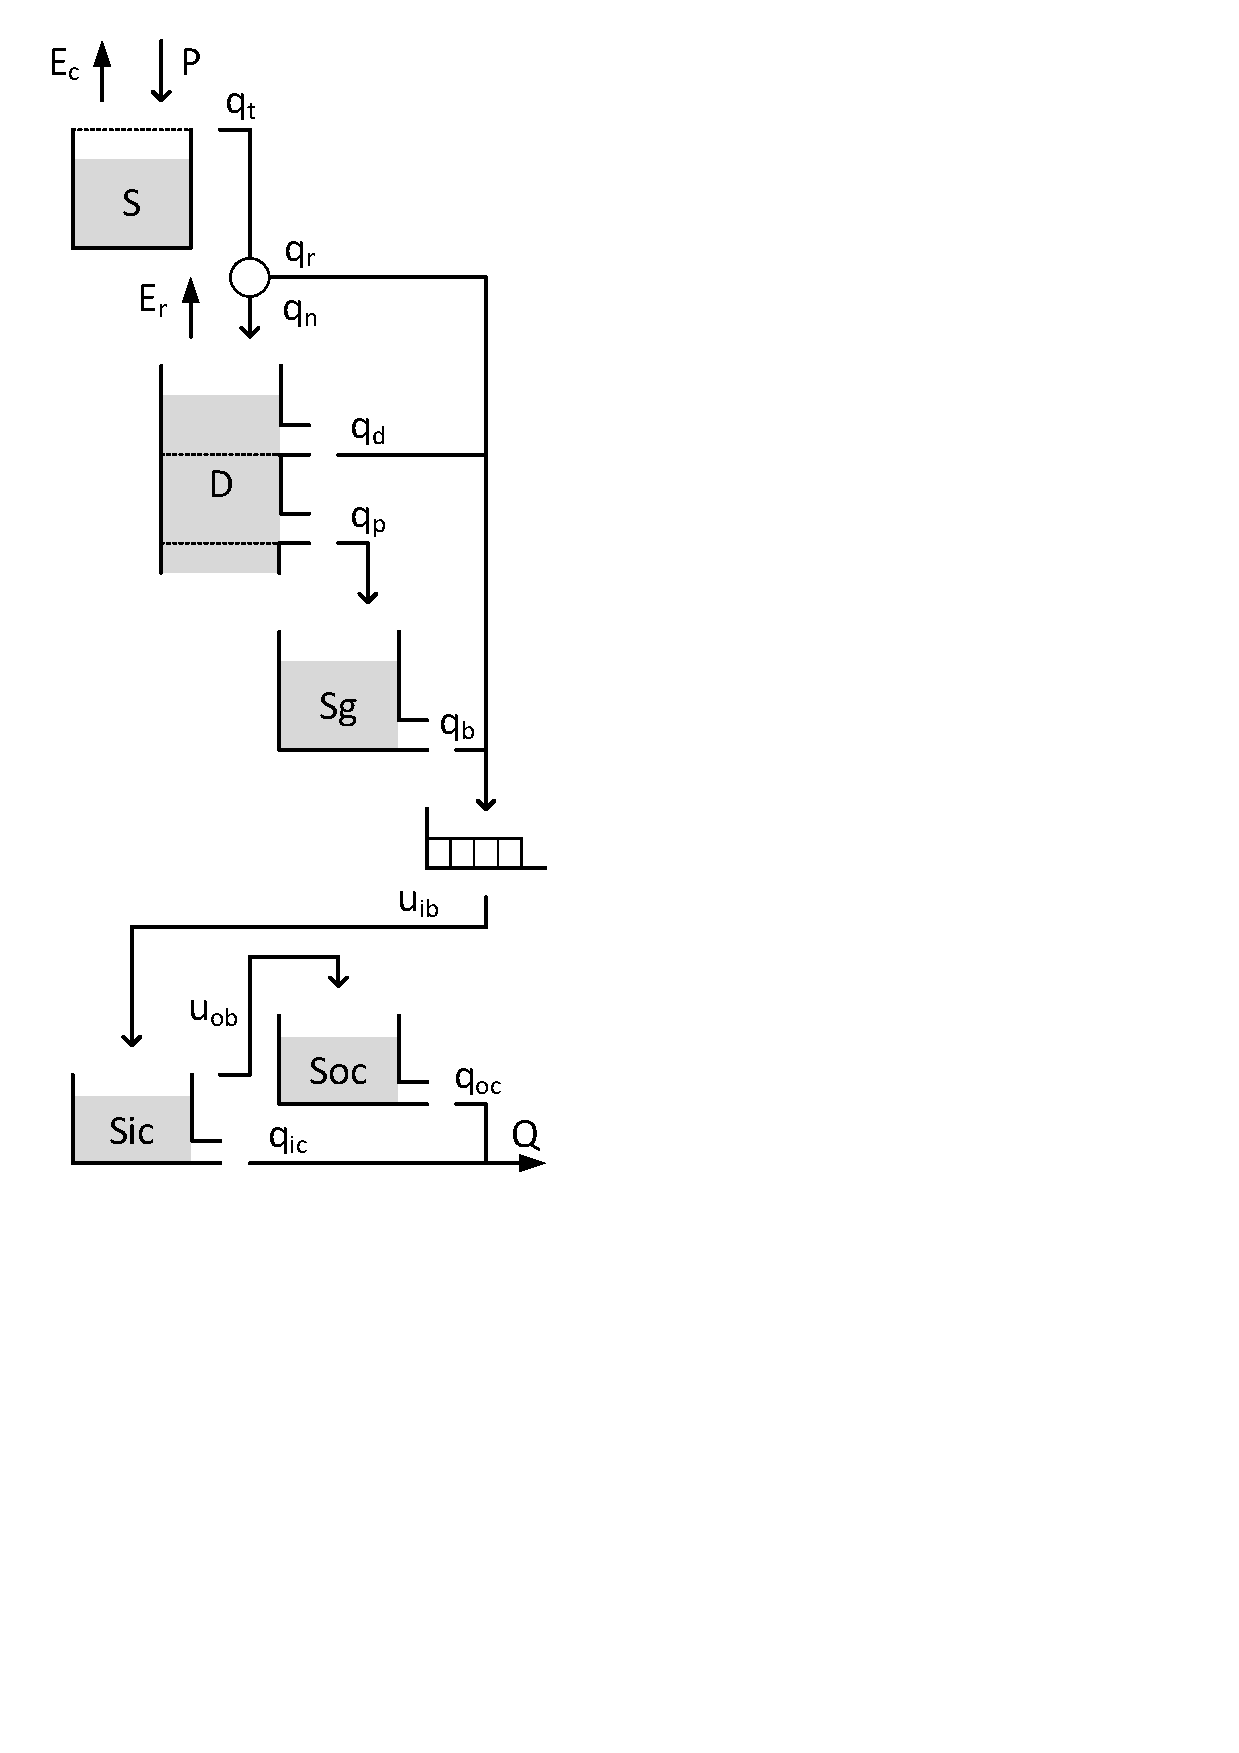
\includegraphics[trim=1cm 10cm 7cm 1cm,width=7cm,keepaspectratio]{./AppA_files/39_schematic.pdf}
\caption{Structure of the MCR model} \label{fig:39_schematic}
\end{wrapfigure}

\begin{align}
	\frac{dS}{dt} &= P-E_c-q_t \\
	E_c &= \begin{cases}
		E_p, &\text{if } S > 0 \\
		0, & \text{otherwise} \\
	\end{cases} \\
	q_t &= 
	\begin{cases}
		P, & \text{if } S=S_{max} \\
		0, & \text{otherwise}
	\end{cases}
\end{align}

Where $S$ [mm] is the current interception storage, refilled by precipitation $P$ $[mm/d]$ and drained by evaporation $E_c$ $[mm/d]$ and throughfall $q_t$ $[mm/d]$.
$E_c$ occurs at the potential rate whenever possible.
$q_t$ occurs only when the store is at maximum capacity $S_{max}$ [mm].

\begin{align}
	\frac{dD}{dt} &= q_n - E_r -q_d-q_p\\
	q_n &=q_t-q_r\\
	q_r &= min\left(c_{max},c_0+c_0e^{c_1D}\right)*q_t\\
	E_r &= \frac{1}{1+e^{-c_eD}}*\left(E_p-E_c\right)\\
	q_d&= \begin{cases}
		k_d\left(D_{surp}-D\right)^{\gamma_d}, &\text{if } D > D_{surp} \\
		0, &\text{otherwise} \\
	\end{cases} \\
	q_p &= \begin{cases}
		q_{p,max}, & \text{if } D\geq D_{surp} \\
		\frac{D}{D_{surp}}q_{p,max}, & \text{if } 0 < D < D_{surp}\\
		0, & \text{otherwise}
	\end{cases}
\end{align}
} % end of wrapfigure fix

Where $D$ [mm] is the current storage in soil moisture, refilled by net infiltration $q_n$ $[mm/d]$ and drained by evaporation $E_r$ $[mm/d]$, direct runoff $q_d$ $[mm/d]$ and percolation $q_p$ $[mm/d]$. 
Negative D-values are possible and indicate a moisture deficit. 
Net inflow $q_n$ is calculated as the difference between throughfall $q_t$ and rapid runoff $q_r$ $[mm/d]$.
$q_r$ varies depending on the current degree of saturation in the catchment, with a maximum fraction of the catchment area contributing to rapid runoff called $c_{max}$ [-], a minimum contributing area of $c_0$ [-] and an exponential increase with increasing soil moisture storage, controlled through shape parameter $c_1$ [-], in between.
$E_r$ fulfils any remaining evaporation demand but decreases with increasing moisture deficit (negative D values).
This relation is controlled through shape parameter $c_2$.
$q_d$ has a non-linear relation with storage above a threshold $D_{surp}$ [mm] through time scale parameter $k_d$ $[d^{-1}]$ and non-linearity parameter $\gamma_d$ [-].
Percolation $q_p$ has a maximum rate of $q_{p,max}$ if D is above threshold $D_{surp}$ and decreases linearly between $D=D_{surp}$ and $D=0$.

\begin{align}	
	\frac{dS_g}{dt} &= q_p - q_b\\
	q_b &= k_g*S_g^{1.5}
\end{align}
  
Where $S_g$ [mm] is the current groundwater storage, refilled by percolation $q_p$ and drained by baseflow $q_b$ $[mm/d]$.
$q_b$ uses time parameter $k_g$ $[d^{-1}]$ and a fixed non-linearity coefficient of 1.5. 
Next, $q_r$, $q_d$ and $q_b$ are summed together and distributed uniformly over timespan $\tau$ [d], giving delayed flow $u_{ib}$ $[mm/d]$.

\begin{align}
	\frac{dS_{ic}}{dt} &= u_{ib} - u_{ob} - q_{ic}\\
	u_{ob} &= \begin{cases}
		u_{ib}, & \text{if } S_{ic}=S_{bf} \\
		0, & \text{otherwise}\\
	\end{cases}\\
	q_{ic} &= \begin{cases}
		k_{cr}*S_{ic}^{\gamma_{cr}}, & \text{if } q_{ic}<\frac{3}{4}S_{ic} \\
		\frac{3}{4}S_{ic}, & \text{otherwise}
	\end{cases}
\end{align}

Where $S_{ic}$ [mm] is the current in-channel storage, refilled by $u_{ic}$ and drained by in-channel flow $q_{ic}$  $[mm/d]$ and out-of-bank flow $u_{ob}$  $[mm/d]$.
$u_{ob}$ only occurs when the store is at maximum capacity $S_{bf}$ [mm].
$q_{ic}$ uses time parameter $k_{cr}$ $[d^{-1}]$ and non-linearity parameter $\gamma_{cr}$ [-].

\begin{align}
	\frac{dS_{oc}}{dt} &= u_{ob} - q_{oc} \\
	q_{oc} &= \begin{cases}
		k_{or}*S_{oc}^{\gamma_{or}}, & \text{if } q_{oc}<\frac{3}{4}S_{oc} \\
		\frac{3}{4}S_{oc}, & \text{otherwise}
	\end{cases} 
\end{align}

Where $S_{oc}$ [mm] is the current out-of-channel storage, refilled by $u_{ob}$ and drained by out-of-channel flow $q_{oc}$  $[mm/d]$.
$q_{oc}$  uses time parameter $k_{or}$ $[d^{-1}]$ and non-linearity parameter $\gamma_{or}$ [-]. Total flow:

\begin{align}
	Q_t &= q_{oc}+q_{ic}
\end{align}

\newpage
\subsection{Parameter overview}
% Table generated by Excel2LaTeX from sheet 'Sheet1'
\begin{table}[htbp]
  \centering
    \begin{tabular}{lll}
    \toprule
    Parameter & Unit  & Description \\
    \midrule
    $S_{max}$ & $mm$  & Maximum interception storage \\
    $c_{max}$ & $-$   & Maximum fraction of area contributing to rapid runoff \\
    $c_0$ & $-$   & Minimum fraction of area contributing to rapid runoff \\
    $c_1$ & $-$   & Contributing area exponential shape parameter \\
    $c_e$ & $-$   & Evaporation exponential shape parameter \\
    $D_{surp}$ & $mm$  & Threshold for direct runoff generation \\
    $k_d$ & $d^{-1}$ & Runoff coefficient \\
    $\gamma_d$ & $-$   & Runoff non-linearity \\
    $q_{p,max}$ & $mm~d^{-1}$ & Maximum percolation rate \\
    $k_g$ & $d^{-1}$ & Runoff coefficient \\
    $\tau$ & $d$   & Unit Hydrograph time base \\
    $S_{bf}$ & $mm$  & Maximum groundwater storage \\
    $k_{cr}$ & $d^{-1}$ & Runoff coefficient \\
    $\gamma_{cr}$ & $-$   & Runoff non-linearity \\
    $k_{or}$ & $d^{-1}$ & Runoff coefficient \\
    $\gamma_{or}$ & $-$   & Runoff non-linearity \\
    \bottomrule
    \end{tabular}%
  \label{tab:addlabel}%
\end{table}%

\subsection{SMAR (model ID: 40)}
The SMAR model (fig.~\ref{fig:40_schematic}) is the result of a series of modifications to the original 'layers-model' \citep{OConnell1970} and summarized by \citet{Tan1996}. The model uses an arbitrary number of soil moistures stores connected in series, with each store having a depth of 25mm. The number of stores is an optimization parameter. The current storage in the upper 5 stores features in various equations. For consistency within this framework, the process is reversed: the model uses a fixed number of 5 soil moisture stores, but the depth of each store is variable and given as $S_{n,max} = S_{max} / 5$. It has 6 stores and 8 parameters ($H$, $Y$, $S_{max}$, $C$, $G$, $K_G$, $N$ and $K$). The model aims to represent:

\begin{itemizecompact}
\item Saturation excess overland flow;
\item Infiltration excess overland flow;
\item Gradual infiltration into soil moisture and declining evaporation potential when water is sourced from further underground;
\item Groundwater flow;
\item Routing of non-groundwater flow.
\end{itemizecompact}

\subsubsection{File names}
\begin{tabular}{@{}ll}
Model: &m\_40\_smar\_8p\_6s \\
Parameter ranges: &m\_40\_smar\_8p\_6s\_parameter\_ ranges \\
\end{tabular}

% Equations
\subsubsection{Model equations}

% Model layout figure
{ 																	% This ensures it doesn't warp text further down
\begin{wrapfigure}{l}{5cm}
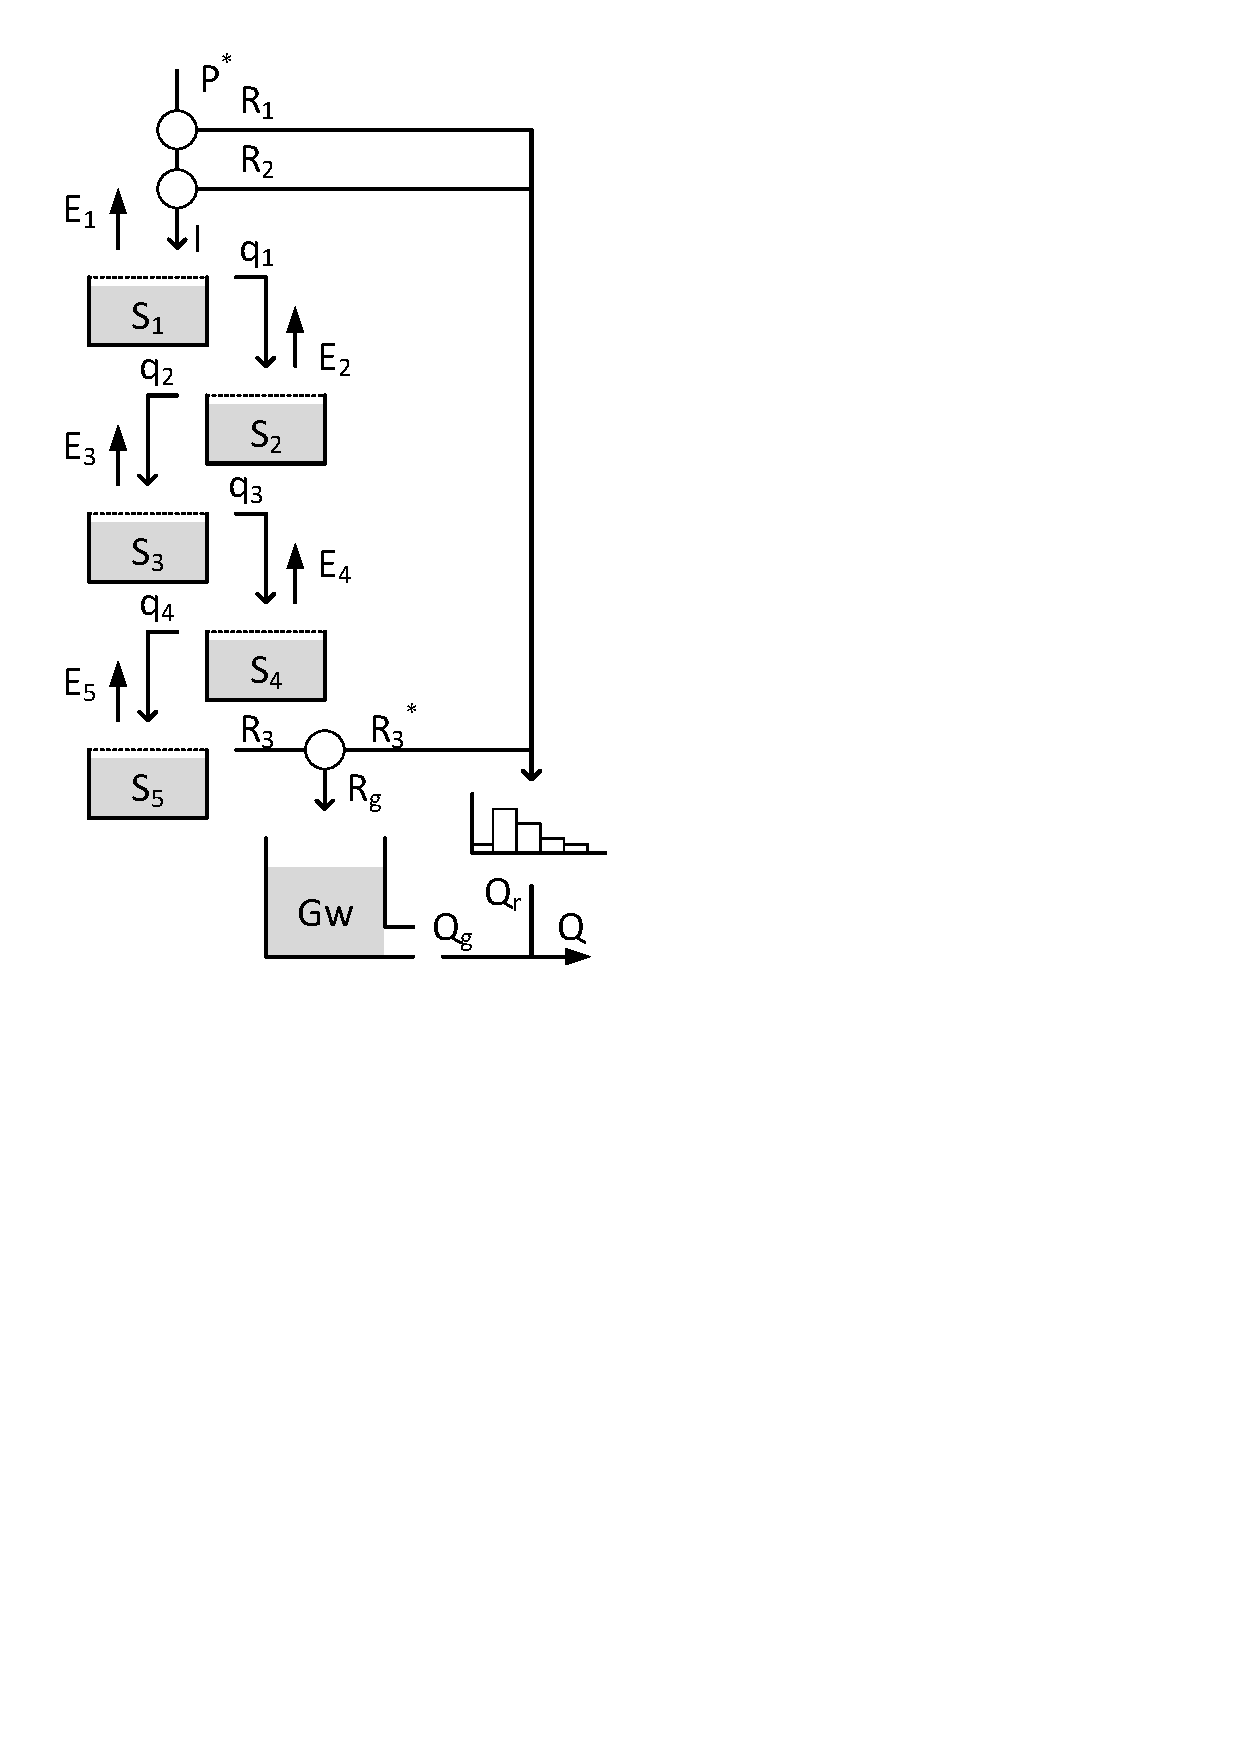
\includegraphics[trim=1cm 13cm 7cm 1cm,width=7cm,keepaspectratio]{./files/40_schematic.pdf}
\caption{Structure of the SMAR model} \label{fig:40_schematic}
\end{wrapfigure}

\begin{align}
	\frac{dS_1}{dt} &= I-E_1-q_1 \\
	I &= \begin{cases}
		Y, &\text{if } P^*-R_1 \geq Y \\
		P^*-R_1, & \text{otherwise} \\
		\end{cases}\\
	P^* &= \begin{cases}
		P-E_p, &\text{if } P > E_p \\
		0, & \text{otherwise} \\
	\end{cases} \\
	R_1 &= P^**H*\frac{\sum{S_n}}{S_{max}}\\
	R_2 &= \left(P^*-R_1\right) - I\\
	E_1 &= C^{(1-1)}*Ep^* \\
	E_p^* &= \begin{cases}
		E_p-P, &\text{if } E_p > P \\
		0, & \text{otherwise} \\
	\end{cases} \\
	q_1 &= 
	\begin{cases}
		P^*-R_1-R_2, & \text{if } S_1 \geq \frac{S_{max}}{5} \\
		0, & \text{otherwise}
	\end{cases}
\end{align}

} %end wrap figure

Where $S_1$ [mm] is the current storage in the upper soil layer, $I$ $[mm/d]$ infiltration into the soil, $P^*$ the effective precipitation $[mm/d]$, $R_1$ $[mm/d]$ is direct runoff, $R_2$ $[mm/d]$ is infiltration excess runoff, $E_1$ $[mm/d]$ evaporation and $q_1$ $[mm/d]$ flow towards deeper soil layers. $I$ uses a constant infiltration rate $Y$ $[mm/d]$. Direct runoff $R_1$ relies on distribution parameter $H$ [-] and is scaled by the current soil moisture storage in all layers compared to the maximum soil moisture storage $S_{max}$ [mm] of all layers. Evaporation from this soil layer occurs at the effect potential rate $E_p^*$. Runoff to deeper layers $q_1$ only occurs when the current storage exceeds the store's maximum capacity. 

\begin{align}
	S_2 &= q_1 - E_2 - q_2\\
	E_2 &= 
		\begin{cases}
		C^{(2-1)}*Ep , & \text{if } S_1 = 0\\
		0, & \text{otherwise}\\
	\end{cases}\\
	q_2 &= 
	\begin{cases}
		q1, & \text{if } S_2 \geq \frac{S_{max}}{5} \\
		0, & \text{otherwise}
	\end{cases}
\end{align}

Where $S_2$ [mm] is the current storage in the second soil layer, $E_2$ $[mm/d]$ the evaporation scaled by parameter $C$ [-], and $q_2$ $[mm/d]$ overflow into the next layer. Evaporation is assumed to occur only when the storage in the upper layers has been exhausted.

\begin{align}
	S_3 &= q_2 - E_3 - q_3\\
	E_3 &= 
		\begin{cases}
		C^{(3-1)}*Ep , & \text{if } S_2 = 0\\
		0, & \text{otherwise}\\
	\end{cases}\\
	q_3 &= 
	\begin{cases}
		q2, & \text{if } S_3 \geq \frac{S_{max}}{5} \\
		0, & \text{otherwise}
	\end{cases}
\end{align}

Where $S_3$ [mm] is the current storage in the second soil layer, $E_3$ $[mm/d]$ the evaporation scaled by parameter $C^2$ [-], and $q_3$ $[mm/d]$ overflow into the next layer. Evaporation is assumed to occur only when the storage in the upper layers has been exhausted.

\begin{align}
	S_4 &= q_3 - E_4 - q_4\\
	E_4 &= 
		\begin{cases}
		C^{(4-1)}*Ep , & \text{if } S_3 = 0\\
		0, & \text{otherwise}\\
	\end{cases}\\
	q_4 &= 
	\begin{cases}
		q3, & \text{if } S_4 \geq \frac{S_{max}}{5} \\
		0, & \text{otherwise}
	\end{cases}
\end{align}

Where $S_4$ [mm] is the current storage in the second soil layer, $E_4$ $[mm/d]$ the evaporation scaled by parameter $C^3$ [-], and $q_4$ $[mm/d]$ overflow into the next layer. Evaporation is assumed to occur only when the storage in the upper layers has been exhausted.

\begin{align}
	S_5 &= q_4 - E_5 - R_3\\
	E_5 &= 
		\begin{cases}
		C^{(5-1)}*Ep , & \text{if } S_4 = 0\\
		0, & \text{otherwise}\\
	\end{cases}\\
	R_3 &= 
	\begin{cases}
		q4, & \text{if } S_5 \geq \frac{S_{max}}{5} \\
		0, & \text{otherwise}
	\end{cases}
\end{align}

Where $S_5$ [mm] is the current storage in the second soil layer, $E_5$ $[mm/d]$ the evaporation scaled by parameter $C^4$ [-], and $R_3$ $[mm/d]$ overflow towards groundwater. Evaporation is assumed to occur only when the storage in the upper layers has been exhausted.

\begin{align}
	\frac{dG_w}{dt} &= R_g -Q_g\\
	R_g &= G*R_3\\
	Q_g &= K_G*G_w
\end{align}

Where $ G_w$ [mm] is the current groundwater storage, refilled by fraction $G$ [-] of $R_3$ $[mm/d]$ and drained as a linear reservoir with time parameter $K_G$ $[d^{-1}]$. This groundwater flow $Q_g$   $[mm/d]$ contributes directly to simulated streamflow $Q$. The fraction $R_3^* = (1-G)*R_3$ that does not reach the groundwater reservoir is combined with $R_1$ and $R_2$ and routed with a gamma function with parameters $N$ and $K$. The routing function approximates a Nash-cascade consisting of $N$ reservoirs with storage coefficient $K$ [d]: 

\begin{align}
 	Q_r &= \left(R_1+R_2+R_3\right)\frac{1}{K\Gamma(N)}\left(\frac{t}{K}\right)^{N-1}e^{-t/K}
\end{align}

Integration over the time step length $d$ provides the fraction of flow routed per time step $Q_r$ $[mm/d]$. Total flow:

\begin{align}
	Q_t = Q_r+Q_g
\end{align}

\newpage
\subsubsection{Parameter overview}
% Table generated by Excel2LaTeX from sheet 'Sheet1'
\begin{table}[htbp]
  \centering
    \begin{tabular}{lll}
    \toprule
    Parameter & Unit  & Description \\
    \midrule
    $H$   & $-$   & Fraction of effective precipitation that is direct runoff \\
    $Y$   & $mm~d^{-1}$ & Infiltration rate \\
    $S_{max}$ & $mm$  & Maximum soil moisture storage \\
    $C$   & $-$   & Evaporation reduction parameter \\
    $G$   & $-$   & Fraction of subsurface flow to groundwater \\
    $K_G$ & $d^{-1}$ & Runoff coefficient \\
    $N$   & $-$   & Gamma function parameter \\
    $K$   & $d$   & Routing time parameter \\
    \bottomrule
    \end{tabular}%
  \label{tab:addlabel}%
\end{table}%

\section{NAM model (model ID: 41)}
The NAM model (fig.~\ref{fig:41_schematic}) is originally developed for use in Denmark \citep{Nielsen1973}. Here a small modification is made by replacing runoff routing equations of the form $\frac{1}{k}e^{-t/k}$ with the linear reservoirs these equations represent. The model has 6 stores and 10 parameters ($C_s$, $C_{if}$, $L^*$, $C_{L1}$, $U^*$, $C_{of}$, $C_{L2}$, $K_0$, $K_1$ and $K_b$). The model aims to represent:

\begin{itemizecompact}
\item Snow accumulation and melt;
\item Interflow when total soil moisture exceeds a threshold;
\item Separation of saturation excess flow into overland flow and infiltration;
\item Baseflow from groundwater.;
\end{itemizecompact}

\subsection{MARRMoT model name}
m\_41\_nam\_10p\_6s \\

% Equations
\subsection{Model equations}

% Model layout figure
{ 																	% This ensures it doesn't warp text further down
\begin{wrapfigure}{l}{6cm}
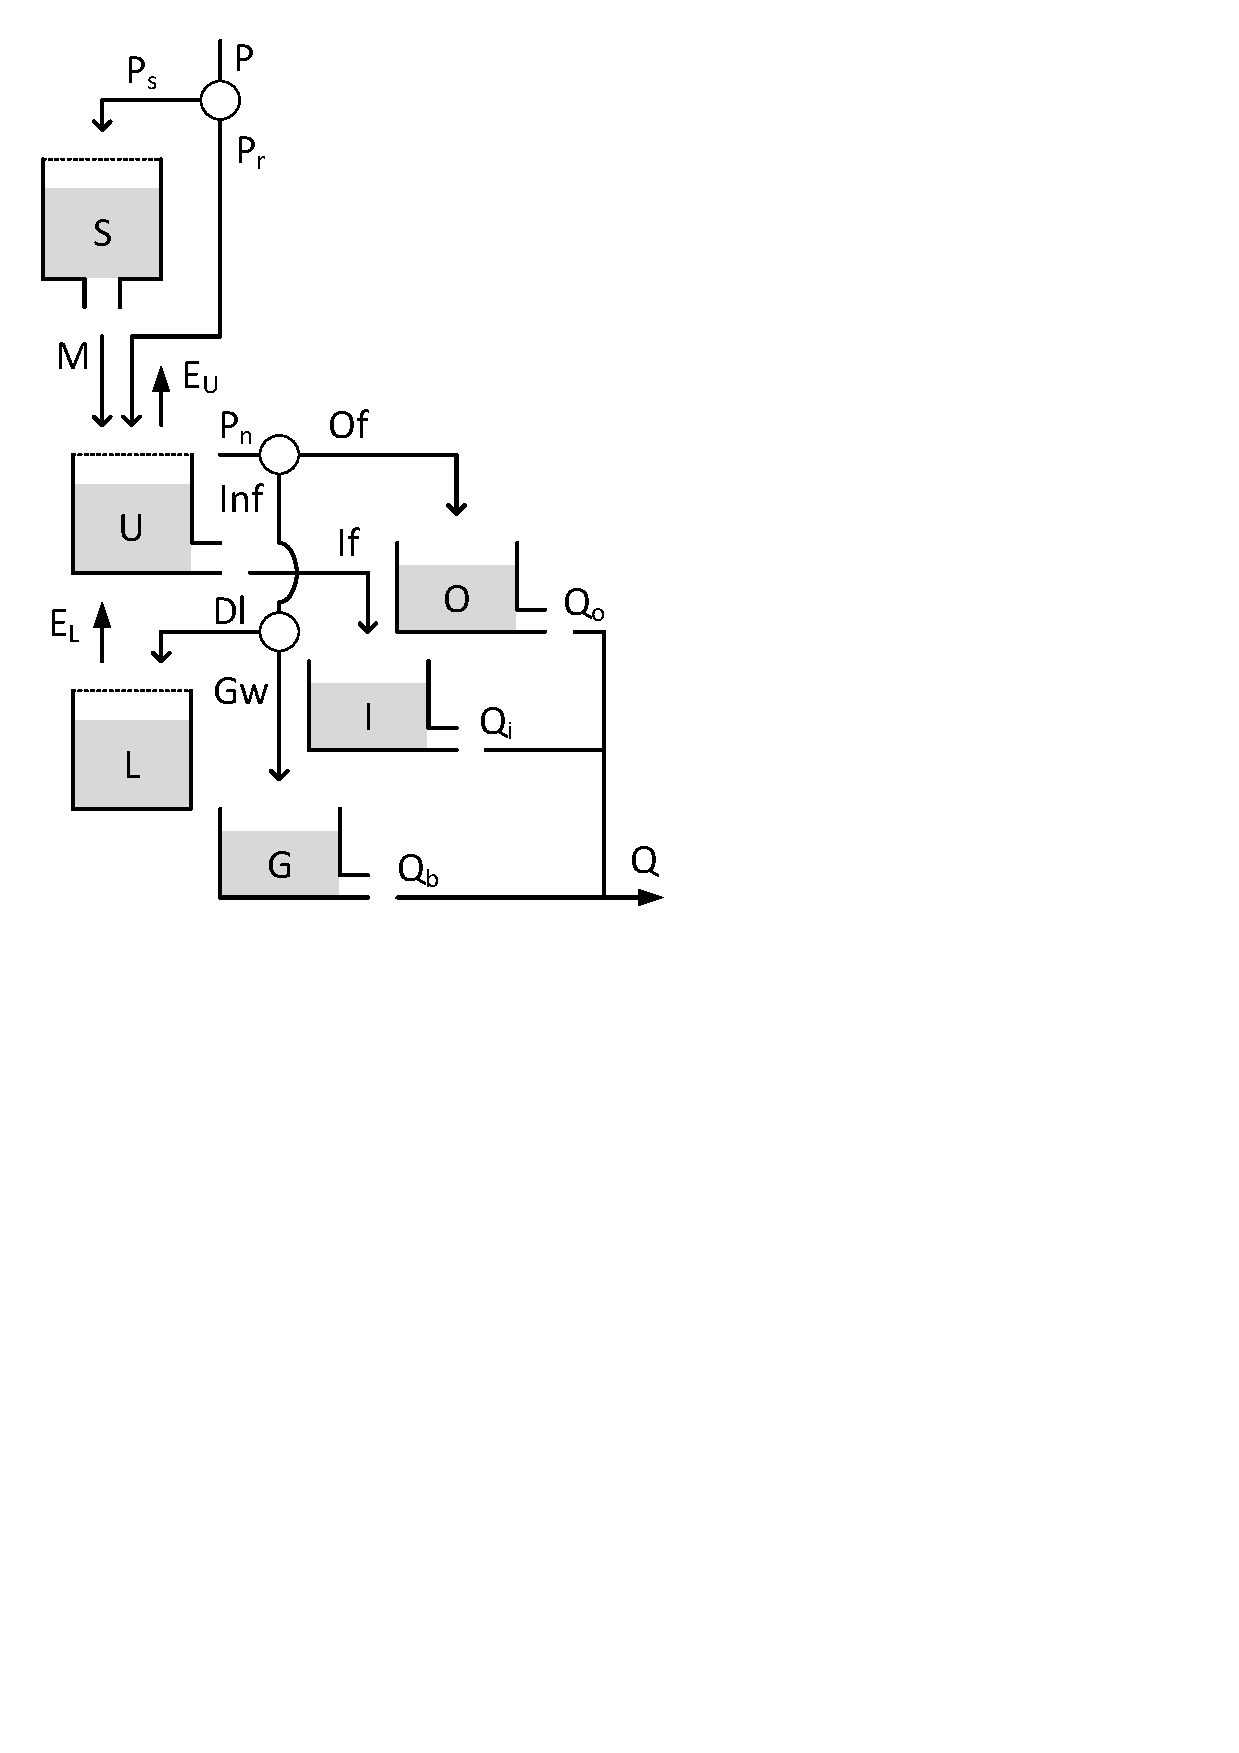
\includegraphics[trim=1cm 14cm 7cm 1cm,width=7cm,keepaspectratio]{./AppA_files/41_schematic.pdf}
\caption{Structure of the NAM model} \label{fig:41_schematic}
\end{wrapfigure}

\begin{align}
	\frac{dS}{dt} &= P_s-M \\
	P_s &= \begin{cases}
		P, &\text{if } T \leq 0 \\
		0, & \text{otherwise} \\
	\end{cases} \\
	M &= 
	\begin{cases}
		C_s*T, & \text{if } T > 0 \\
		0, & \text{otherwise}
	\end{cases}
\end{align}

Where $S$ is the current snow storage [mm], $P_s$ $[mm/d]$ the precipitation that falls as snow and M the snowmelt $[mm/d]$ based on a degree-day factor ($c_s$, [mm/\degree C/d]). The freezing point of $0^o$ [C] is used as a threshold for snowfall and melt.

} % end of wrapfigure fix

\begin{align}
	\frac{dU}{dt} &= P_r + M -E_U - If - P_n\\
	P_r &= \begin{cases}
		P, &\text{if } T > 0 \\
		0, & \text{otherwise} \\
	\end{cases} \\
	E_U &= \begin{cases}
		E_p, &\text{if } U > 0 \\
		0, &\text{otherwise} \\
	\end{cases} \\
	If &= \begin{cases}
		C_{if}*\frac{L/L^*-C_{L1}}{1-C_{L1}}U, &\text{if } L/L^* > C_{L1}\\
		0, &\text{otherwise}\\
	\end{cases}\\
	P_n &= \begin{cases}
		(P_r + M), &\text{if } U = U^*\\
		0, &\text{otherwise}\\
	\end{cases}	
\end{align}

Where U [mm] is the current storage in the upper zone, refilled by precipitation as rain $P_r$ $[mm/d]$ and snowmelt $M$, and drained by evaporation $E_U$ $[mm/d]$, interflow $If$ $[mm/d]$ and net precipitation $P_n$ $[mm/d]$. 
$P_r$ occurs only when the current temperature exceeds the threshold of $0^o$C. 
$E_U$ occurs at the potential rate $E_p$ whenever possible. 
$If$ occurs only if the fractional storage in the lower zone $L/L^*$ ($L$ is current lower zone storage, $L^*$ is lower zone maximum storage) exceeds a threshold $C_{L1}$ [-]. 
$If$ is scaled by the current deficit in the lower zone and a uses runoff coefficient $C_{if}$ [-]. 
$P_n$ occurs only when the upper zone exceeds its maximum storage capacity $U^*$ [mm].

\begin{align}
	\frac{dL}{dt} &= Dl - E_t \\
	Dl &= (P_n - Of)\left(1-\frac{L}{L^*}\right)\\
	Of &= \begin{cases}
		C_{of}*\frac{L/L^*-C_{L2}}{1-C_{L2}}*P_n, &\text{if } L/L^* > C_{L2}\\
		0, &\text{otherwise}\\
	\end{cases}\\
	E_t &=\begin{cases}
		 \frac{L}{L^*}E_p, &\text{if } U = 0\\
		0, &\text{otherwise}\\
	\end{cases}
\end{align}
  
Where $L$ [mm] is the current storage in the lower zone, refilled by a fraction of infiltration $Dl$ $[mm/d]$ and drained by evaporation $E_t$ $[mm/d]$. $Dl$ is calculated as a fraction of infiltration $P_n -Of$, dependent on the current deficit in the lower zone. 
Note that with the current formulation $Dl$ might be larger than the lower zone deficit $L^*-L$ and a constraint of the form $Dl \leq L^*-L$ is needed.
 Overland flow $Of$ $[mm/d]$ is a fraction of $P_n$ determined using the relative storage in the lower zone $L/L^*$ and two coefficients $C_{of}$ [-] and $C_{L2}$ [-]. 
$E_t$ occurs only when the upper zone is empty, and at a reduced rate that uses the relative storage in the lower zone.

\begin{align}
	\frac{dO}{dt} &= Of - Q_o\\
	Q_o &= K_0 * O 
\end{align}

Where $O$ [mm] is the current storage in the overland flow routing store.
$Q_o$ is the routed overland flow, using time coefficient $K_0$ $[d^{-1}]$.

\begin{align}
	\frac{dI}{dt} &= If - Q_i\\
	Q_i &= K_1 * I 
\end{align}

Where $I$ [mm] is the current storage in the interflow routing store.
$Q_i$ is the routed interflow, using time coefficient $K_1$ $[d^{-1}]$.

\begin{align}
	\frac{dG}{dt} &= Gw - Q_b\\
	Gw &= (P_n-Of)\left(\frac{L}{L^*}\right)\\
	Q_b &= K_b * O 
\end{align}

Where $G$ [mm] is the current storage in the overland flow routing store, refilled by groundwater flow $Gw$ $[mm/d]$.
$Q_b$ is the routed baseflow, using time coefficient $K_b$ $[d^{-1}]$. Total flow:

\begin{align}
	Q &= Q_o+Q_i+Q_b
\end{align}


\subsection{Parameter overview}
% Table generated by Excel2LaTeX from sheet 'Sheet1'
\begin{table}[htbp]
  \centering
    \begin{tabular}{lll}
    \toprule
    Parameter & Unit  & Description \\
    \midrule
    $C_s$ & $mm~^oC^{-1}~d^{-1}$ & Degree-day factor \\
    $C_{if}$ & $d^{-1}$ & Runoff coefficient \\
    $L^*$ & $mm$  & Maximum lower zone storage \\
    $C_{L1}$ & $-$   & Fractional threshold for interflow generation \\
    $U^*$ & $mm$  & Maximum upper zone storage \\
    $C_{of}$ & $d^{-1}$ & Runoff coefficient \\
    $C_{L2}$ & $-$   & Fractional threshold for overland flow generation \\
    $K_0$ & $d^{-1}$ & Runoff coefficient \\
    $K_1$ & $d^{-1}$ & Runoff coefficient \\
    $K_b$ & $d^{-1}$ & Runoff coefficient \\
    \bottomrule
    \end{tabular}%
  \label{tab:addlabel}%
\end{table}%


\section{HYCYMODEL (model ID: 42)}
The HYCYMODEL (fig.~\ref{fig:00_schematic}) is originally developed for use in heavily forested catchments in Japan \citep{Fukushima1988}. The original model specifies evaporation from the $S_b$ store as $E_T = e_p(i)*Q_b/Q_{bc}, \text{ if } S_u < 0 ~\&~ S_b < S_{bc}$, with $Q_{bc} = f(S_{bc})$. However, no further details are given and $S_{bc}$ is not listed as a parameter. We assume that $S_{bc}$ [mm] is a threshold  parameter and that evaporation potential declines linearly to zero when the store drops under this threshold. The model has 6 stores and 12 parameters ($C$, $I_{1,max}$, $\alpha$, $I_{2,max}$, $k_{in}$, $D_{50}$, $D_{16}$, $S_{bc}$, $k_b$, $p_b$, $k_h$ and $k_c$). The model aims to represent:

\begin{itemizecompact}
\item Split between channel and ground precipitation;
\item Interception by canopy and stems/trunks;
\item Overland flow from a variable contributing area;
\item Non-linear channel flow, hillslope flow and baseflow;
\item Channel evaporation.
\end{itemizecompact}

\subsection{MARRMoT model name}
m\_42\_hycymodel\_12p\_6s \\

% Equations
\subsection{Model equations}

% Model layout figure
{ 																	% This ensures it doesn't warp text further down
\begin{wrapfigure}{l}{7cm}
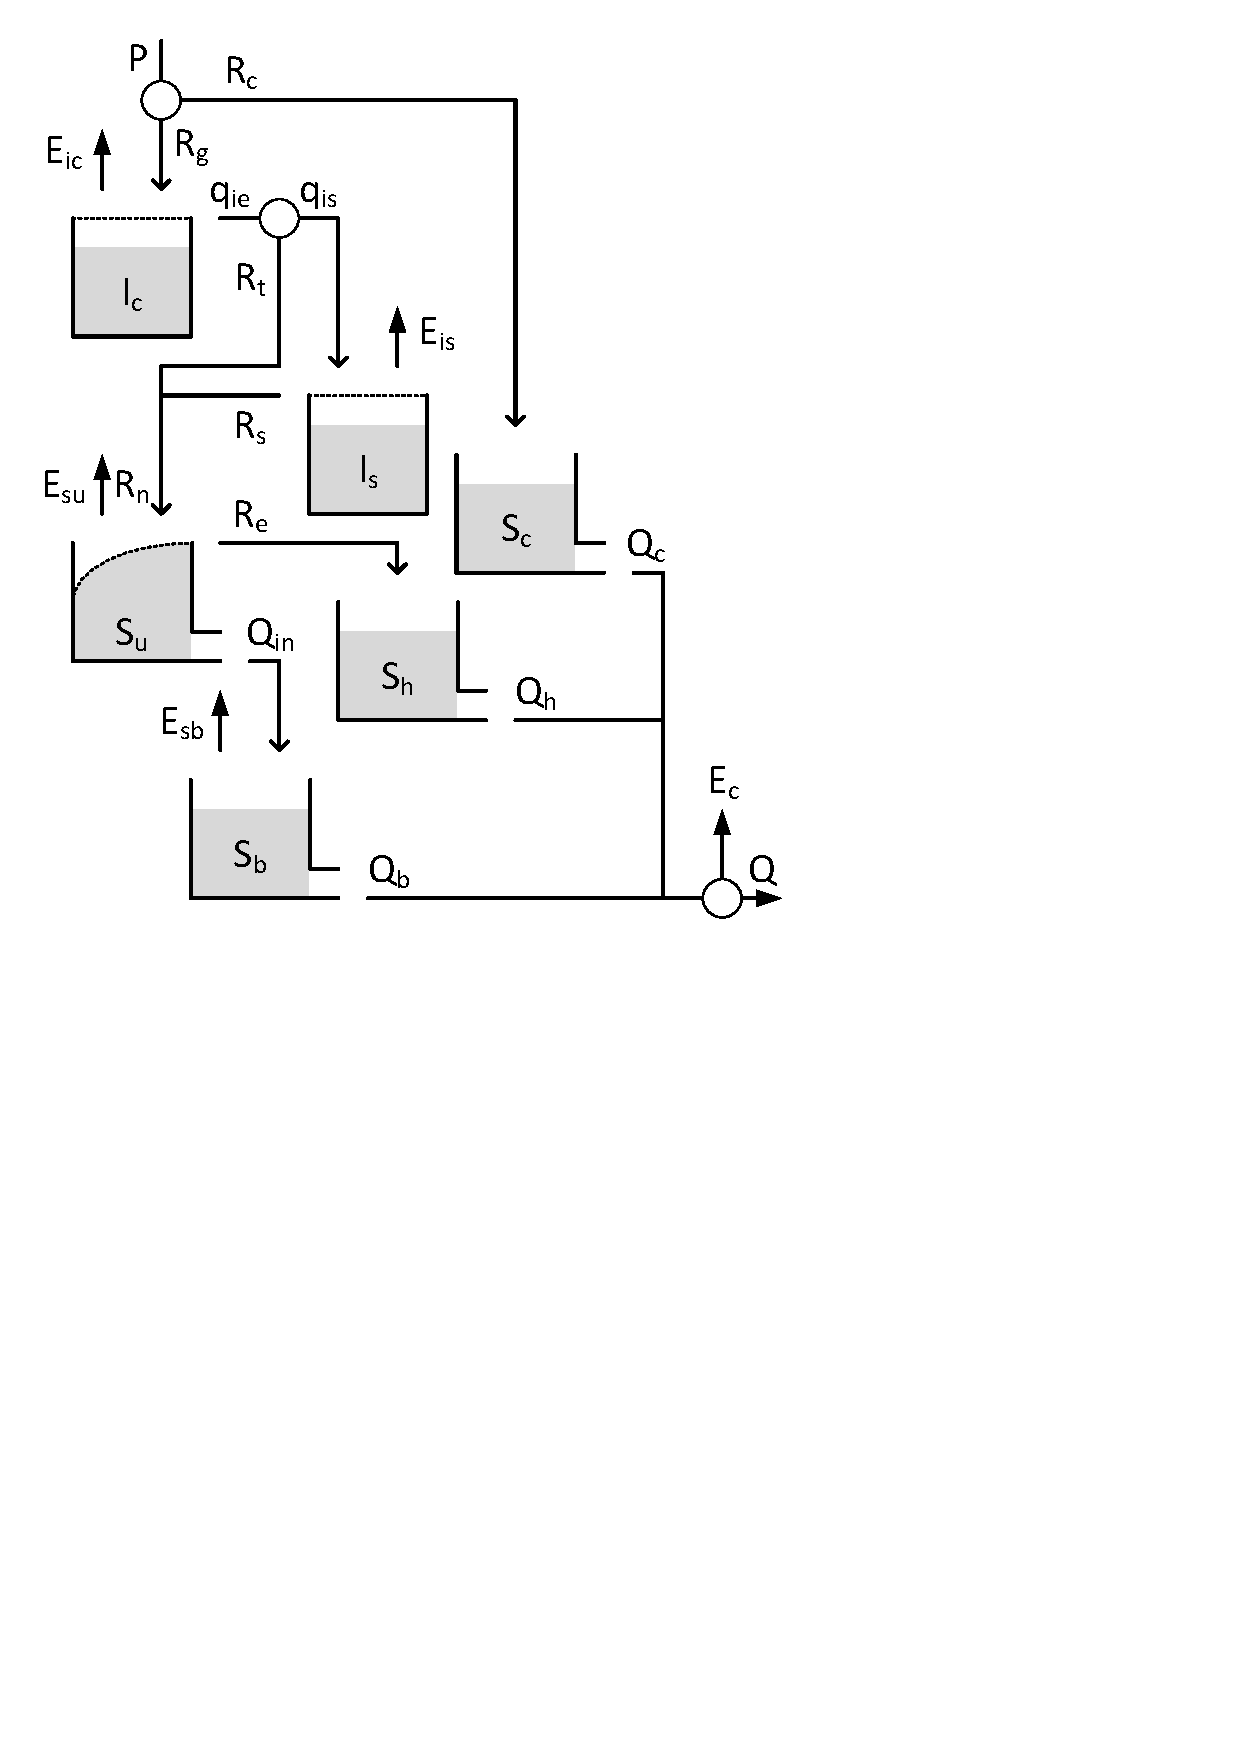
\includegraphics[trim=1cm 14.5cm 7cm 1cm,width=7cm,keepaspectratio]{./AppA_files/42_schematic.pdf}
\caption{Structure of the HYCYMODEL} \label{fig:00_schematic}
\end{wrapfigure}

\begin{align}
	\frac{dI_c}{dt} &= R_g-E_{ic} -q_{ie} \\
	R_g &= (1-C)P\\
	E_{ic} &= 
	\begin{cases}
		(1-C)*E_p, & \text{if } I_c > 0 \\
		0, & \text{otherwise}
	\end{cases}\\
	q_{ie} &= 	\begin{cases}
		R_g, & \text{if } I_c = I_{1,max} \\
		0, & \text{otherwise}
	\end{cases}
\end{align}

Where $I_c$ [mm] is the current canopy storage, refilled by rainfall on ground $R_g$ $[mm/d]$ and drained by evaporation $E_{ic}$ $[mm/d]$ and canopy interception excess $Q_{ie}$ $[mm/d]$.
$R_g$ is the fraction (1-C) [mm] of rainfall $P$ $[mm/d]$ that falls on ground (and not in the channel).
This fraction appears several times in the model to scale evaporation values according to surface area.

} % end of wrapfigure fix

\noindent$E_{ic}$ occurs at the potential rate $E_p$ $[mm/d]$ when possible.
$q_{ie}$ only occurs when the canopy store is at maximum capacity $I_{1,max}$ [mm].

\begin{align}
	\frac{dI_s}{dt} &= q_{is} - E_{is}  - R_s\\
	q_{is} &= \alpha*q_{ie} \\
	E_{is} &= \begin{cases}
		(1-C)*E_p, &\text{if } I_s > 0 \\
		0, &\text{otherwise} \\
	\end{cases} \\
	R_s &= \begin{cases}
		q_{is}, &\text{if } I_s = I_{2,max}\\
		0, &\text{otherwise}\\
	\end{cases}	
\end{align}

Where $I_s$ [mm] is the current stem and trunk storage, refilled by a fraction of canopy excess $q_{is}$ $[mm/d]$ and drained by evaporation $E_{is}$ $[mm/d]$ and stem flow $R_s$ $[mm/d]$.
$q_{is}$ is the fraction $\alpha$ [-] of canopy excess $q_{ie}$.
The remainder $(1-\alpha)$ is throughfall $R_t$ $[mm/d]$.
$E_{is}$ occurs at the potential rate $E_p$ when possible.
$R_s$ occurs only when the store is at maximum capacity $I_{2,max}$ [mm].

\begin{align}
	\frac{dS_u}{dt} &= R_n - Re - E_{su} - Q_{in} \\
	R_n &= R_t + R_s \\
	Re &= m*R_n \\
	m &= \int_{-\inf}^{\xi}\frac{1}{\sqrt{2\pi}}exp\left(-\frac{\xi^2}{2}\right)d\xi\\
	\xi &= \frac{log\left(S_u/D_{50}\right)}{log\left(D_{50}/D_{16}\right)}\\
	E_{su} &= \begin{cases}
		(1-C)*E_p, &\text{if } E_{us} > 0 \\
		0, &\text{otherwise} \\
	\end{cases} \\
	Q_{in} &= k_{in} *S_u
\end{align}

Where $S_u$ [mm] is the current storage in the upper zone, refilled by net precipitation $R_n$ $[mm/d]$ and drained by effective rainfall $R_e$ $[mm/d]$, evaporation $E_{su}$ $[mm/d]$ and infiltration $Q_{in}$ $[mm/d]$.
$R_n$ is the sum of throughfall $R_t$ and stem flow $R_s$.
$R_e$ is a fraction $m$ [-] of $R_e$, determined from a variable contributing area concept.
$m$ is calculated is an integral from a regular normal distribution, scaled by the current storage $S_u$ compared to two parameters $D_{50}$ [mm] and $D_{16}$ [mm].
These parameters represent the effective soil depths at which respectively 50\% and 16\% of the catchment area contribute to $R_e$.
$E_{su}$ occurs at the potential rate $E_p$ when possible.
$Q_{in}$ has a linear relation with storage through time parameter $k_{in}$ $[d^{-1}]$.

\begin{align}
	\frac{dS_b}{dt} &= Q_{in} - E_{sb} - Q_b \\
	E_{sb} &= \begin{cases}
		(1-C)*E_p, &\text{if } S_u = 0  ~\&~ S_b \geq S_{bc} \\
		(1-C)*E_p\frac{S_b}{S_{bc}}, &\text{otherwise} \\
	\end{cases} \\
	Q_b &= k_b*S_b^{p_b}
\end{align}

Where $S_b$ [mm] is the current storage in the lower zone, refilled by infiltration $Q_{in}$ and drained by evaporation $E_{sb}$ $[mm/d]$ and baseflow $Q_b$ $[mm/d]$.
$E_{sb}$ occurs at the potential rate when the store is above a threshold $S_{bc}$ [mm], and declines linearly below that.
$Q_b$ has a potentially non-linear relation with storage through time parameter $k_b$ $[d^{-1}]$ and scale parameter $p_b$ [-].

\begin{align}
	\frac{dS_h}{dt} &= R_e - Q_h \\
	Q_h &=  k_h*S_h^{p_h}
\end{align}

Where $S_h$ [mm] is the current storage in the hillslope routing store, refilled by effective rainfall $R_e$ and drained by hillslope runoff $Q_h$.
$Q_h$ has a potentially non-linear relation with storage through time parameter $k_h$ $[d^{-1}]$ and scale parameter $p_h$ [-].
$p_h$ is a fixed parameter in the original model with value $5/3$.

\begin{align}
	\frac{dS_c}{dt} &= R_c - Q_c \\
	Q_c &=  k_c*S_c^{p_c}
\end{align}

Where $S_c$ [mm] is the current storage in the channel routing store, refilled by rainfall on the channel $R_c$ and drained by channel runoff $Q_c$.
$Q_c$ has a potentially non-linear relation with storage through time parameter $k_c$ $[d^{-1}]$ and scale parameter $p_c$ [-].
$p_c$ is a fixed parameter in the original model with value $5/3$.

\begin{align}
	Q_t &= Q_c+Q_h+Q_b-E_c \\
	E_c &= C*E_p
\end{align}

Where $Q_t$ $[mm/d]$ is the total flow as sum of the three individual flow fluxes minus channel evaporation $E_c$ $[mm/d]$. 

\newpage
\subsection{Parameter overview}
% Table generated by Excel2LaTeX from sheet 'Sheet1'
\begin{table}[htbp]
  \centering
    \begin{tabular}{lll}
    \toprule
    Parameter & Unit  & Description \\
    \midrule
    $C$   & $-$   & Fraction of area that is channel \\
    $I_{1,max}$ & $mm$  & Maximum interception storage \\
    $\alpha$ & $-$   & Fraction of interception excess to stem flow \\
    $I_{2,max}$ & $mm$  & Maximum trunk and stem storage \\
    $k_{in}$ & $d^{-1}$ & Runoff coefficient \\
    $D_{50}$ & $mm$  & Effective soil depth at which 50\% of area contributes to flow \\
    $D_{16}$ & $mm$  & Effective soil depth at which 16\% of area contributes to flow \\
    $S_{bc}$ & $mm$  & Threshold for evaporation behaviour change \\
    $k_b$ & $d^{-1}$ & Runoff coefficient \\
    $p_b$ & $-$   & Runoff non-linearity \\
    $k_h$ & $d^{-1}$ & Runoff coefficient \\
    $k_c$ & $d^{-1}$ & Runoff coefficient \\
    \bottomrule
    \end{tabular}%
  \label{tab:addlabel}%
\end{table}%


\section{GSM-SOCONT model (model ID: 43)}
The Glacier and SnowMelt - SOil CONTribution model (GSM-SOCONT) model (fig.~\ref{fig:43_schematic}) is a model developed for alpine, partly glaciated catchments \citep{Schaefli2005}. For consistency with other models in this framework, several simplifications are used. The model does not use different elevation bands nor DEM data to estimate certain parameters, and does not calculate an annual glacier mass balance. The model has 6 stores and 12 parameters ($f_{ice}$, $T_0$, $a_{snow}$, $T_m$, $k_s$, $a_{ice}$, $k_i$, $A$, $x$, $y$, $k_{sl}$ and $\beta$). The model aims to represent:

\begin{itemizecompact}
\item Separate treatment of glacier and non-glacier catchment area;
\item Snow accumulation and melt;
\item Glacier melt;
\item Soil moisture accounting in the non-glacier catchment area.
\end{itemizecompact}

\subsection{MARRMoT model name}
m\_43\_gsmsocont\_12p\_6s \\

% Equations
\subsection{Model equations}

% Model layout figure
{ 																	% This ensures it doesn't warp text further down
\begin{wrapfigure}{l}{7.5cm}
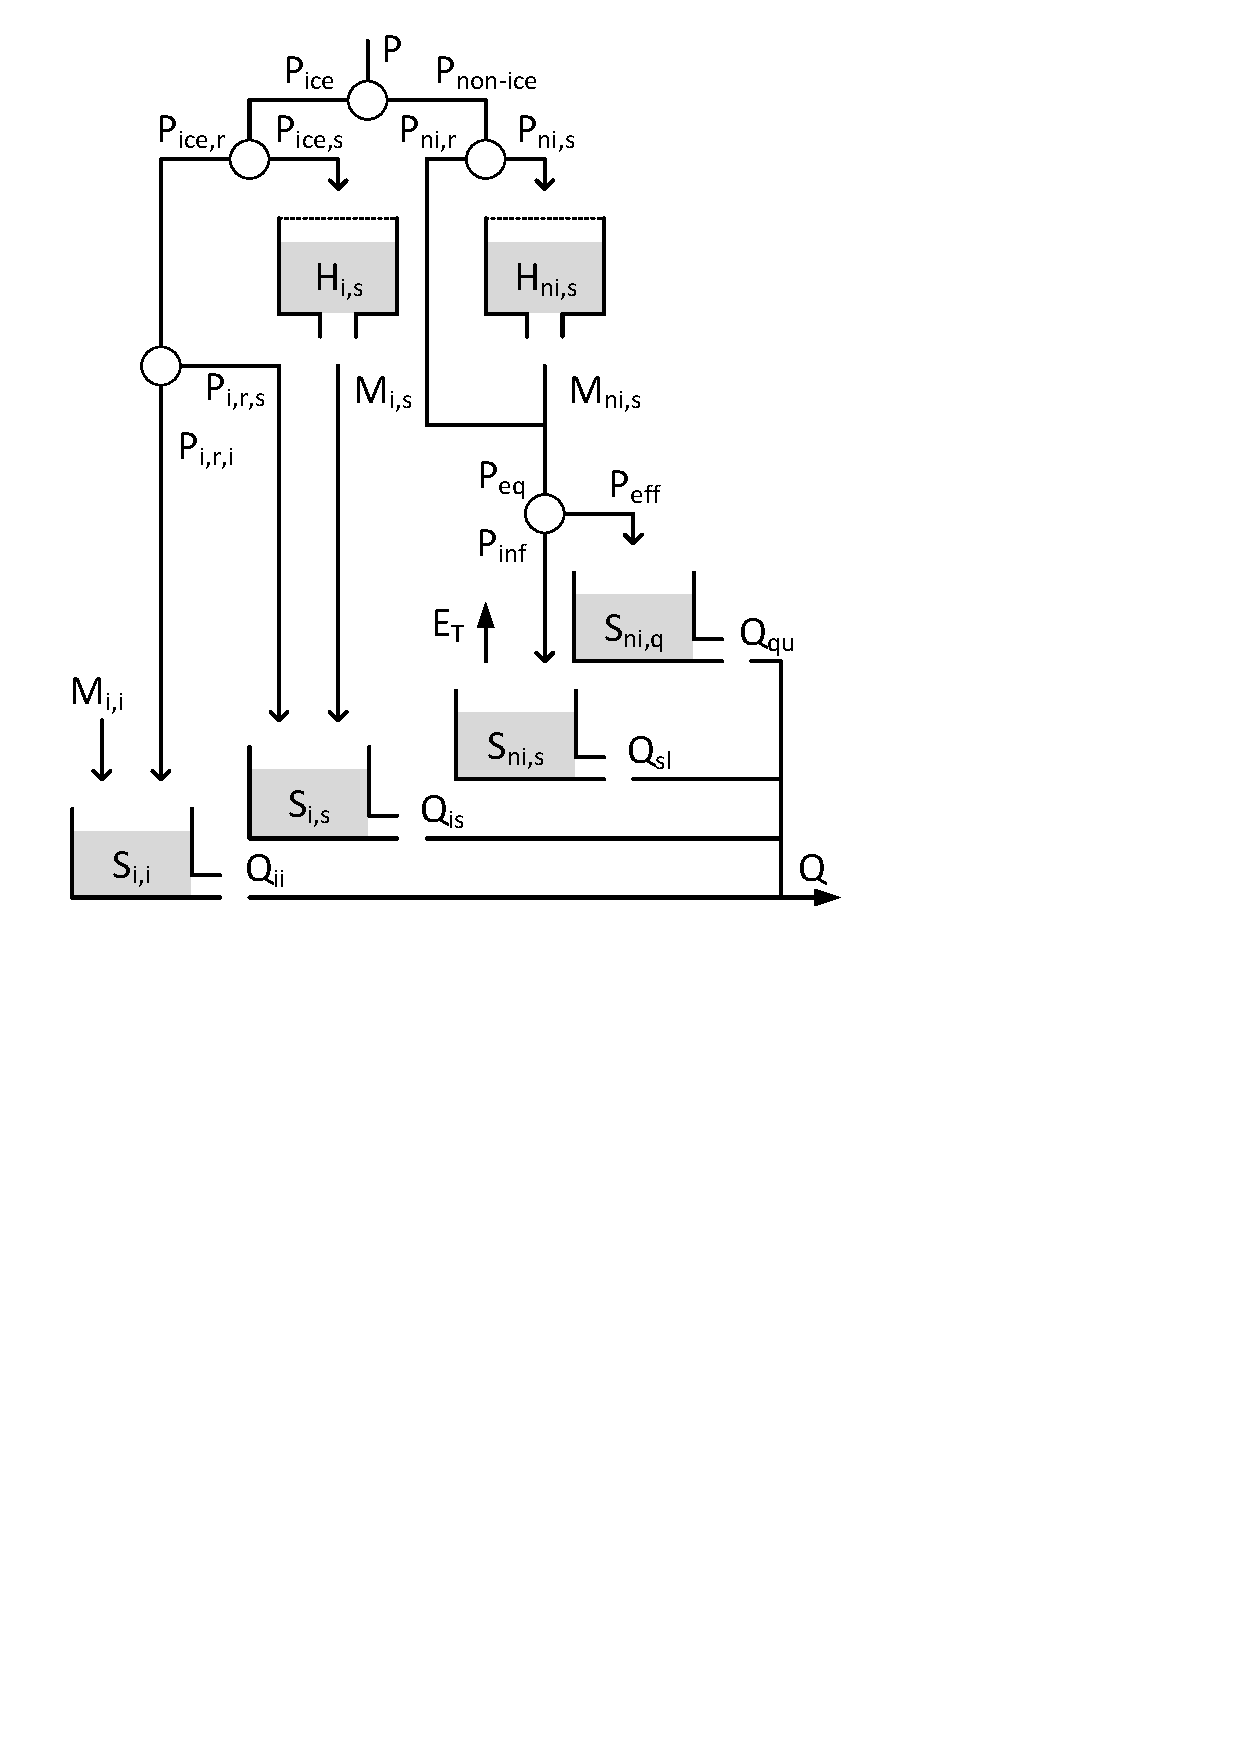
\includegraphics[trim=1cm 14cm 7cm 1cm,width=7cm,keepaspectratio]{./AppA_files/43_schematic.pdf}
\caption{Structure of the GSM-SOCONT model} \label{fig:43_schematic}
\end{wrapfigure}

\begin{align}
	\frac{dH_{i,s}}{dt} &= P_{ice,s} - M_{i,s}\\
	P_{ice,s} &= \begin{cases}
		P_{ice}, &\text{if } T \leq T_0 \\
		0, & \text{otherwise} \\
	\end{cases} \\
	P_{ice} &= f_{ice}*P \\
	M_{i,s} &= \begin{cases}
		a_{snow}(T-T_m), &\text{if } T > T_m \\
		0, &\text{otherwise} 
	\end{cases} 
\end{align}

Where $H_{i,s}$ [mm] is the current storage in the snow pack, refilled by precipitation-as-snow $P_{ice,s}$ $[mm/d]$ and depleted by melt $M_{i,s}$ $[mm/d]$.
$P_{ice,s}$ occurs only when the temperature $T$ $[^oC]$ is below a threshold temperature for snowfall $T_0$ $[^oC]$.
$P_{ice}$ is the fraction $f_{ice}$ [-] of precipitation $P$ $[mm/d]$ that falls on the ice-covered part of the catchment.
$M_{i,s}$ uses a degree-day-factor $a_{snow}$ $[mm/^oC/d]$ to estimate snow melt if temperature is above a threshold for snow melt $T_s$ $[^oC]$.

} % end of wrapfigure fix

\begin{align}
	\frac{dS_{i,s}}{dt} &= M_{i,s} +P_{i,r,s,} -Q_{is}\\
	P_{i,r,s} &= P_{ice,r}, \quad \text{if } H_{i,s} > 0 \\
	P_{ice,r} &= \begin{cases}
		P_{ice}, &\text{if } T > T_0 \\
		0, & \text{otherwise} \\
	\end{cases} \\
	Q_{is} &= k_s*S_{i,s}
\end{align}
  
Where $S_{i,s}$ [mm] is the current storage in the snow-water routing reservoir, refilled by snow melt $M_{i,s}$ $[mm/d]$ and rain-on-snow $P_{ice,s}$ $[mm/d]$, and drained by runoff $Q_{is}$.
$P_{i,r,s}$ occurs only if the current snow pack storage is above zero.
$P_{ice,r}$ is precipitation-as-rain that occurs only if the temperature is above a snowfall threshold $T_0$.
$Q_{is}$ has a linear relation with storage through time parameter $k_s$ $[d^{-1}]$.

\begin{align}
	\frac{dS_{i,i}}{dt} &= M_{i,i} +P_{i,r,i,} -Q_{ii}\\
	P_{i,r,i} &= P_{ice,r}, \quad \text{if } H_{i,s} = 0 \\
	M_{i,s} &= \begin{cases}
		a_{ice}(T-T_m), &\text{if } T > T_m ~\&~ H_{i,s} = 0 \\
		0, &\text{otherwise} \\
	\end{cases}  \\
	Q_{ii} &= k_i*S_{i,i}
\end{align}

Where $S_{i,i}$ [mm] is the current storage in the ice-water routing reservoir, refilled by glacier melt $M_{i,i}$ $[mm/d]$ and rain-on-ice $P_{ice,i}$ $[mm/d]$, and drained by runoff $Q_{ii}$ $[mm/d]$.
Both $M_{i,i}$ and $P_{ice,i}$ are assumed to only occur once the snow pack $H_{i,s}$ is depleted.
$M_{i,i}$ uses a degree-day-factor $a_{ice}$ $[mm/^oC/d]$ to estimate glacier melt. 
Ice storage in the glacier is assumed to be infinite.
$P_{ice,r,i}$ is equal to $P_{ice,r}$ if $H_{i,s} = 0$.
$Q_{ii}$ has a linear relation with storage through time parameter $k_i$ $[d^{-1}]$.

\begin{align}
	\frac{dH_{ni,s}}{dt} &= P_{ni,s} - M_{ni,s}\\
	P_{ni,s} &= \begin{cases}
		P_{non-ice}, &\text{if } T \leq T_0 \\
		0, & \text{otherwise} \\
	\end{cases} \\
	P_{non-ice} &= (1-f_{ice})*P \\
	M_{ni,s} &= \begin{cases}
		a_{snow}(T-T_m), &\text{if } T > T_m \\
		0, &\text{otherwise} 
	\end{cases} 
\end{align}

Where $H_{ni,s}$ [mm] is the current snow pack storage on the non-ice covered fraction $1-f_{ice}$ [-] of the catchment, which increases through snowfall $P_{ni,s}$ $[mm/d]$ and decreases through snow melt $M_{ni,s}$ $[mm/d]$.
Both fluxes are calculated in the same manner as those on the ice-covered part of the catchment (fluxes $P_{ice,s}$ and $M_{ice,s}$).

\begin{align}
	\frac{dS_{ni,s}}{dt} &= P_{inf} - E_T - Q_{sl}\\
	P_{inf} &= P_{eq} -P_{eff} \\
	P_{eff} &= P_{eq}\left(\frac{S_{ni,s}}{A}\right)^y \\	
	P_{eq} &= M_{ni,s} + P_{ni,r} \\
	E_T &= E_p\left( \frac{S_{ni,s}}{A}\right)^x \\
	Q_{sl} &= k_{sl}S_{ni,s}
\end{align}

Where $S_{ni,s}$ [mm] is the current storage in soil moisture, refilled by infiltrated precipitation $P_{inf}$ $[mm/d]$ and drained by evapotranspiration $E_T$ $[mm/d]$ and slow flow $Q_{sl}$ $[mm/d]$.
$P_{inf}$ depends on the effective precipitation $P_{eff}$. 
$P_{eq}$ is the total of snow melt $M_{ni,s}$ and precipitation-as-rain $P_{ni,r}$ $[mm/d]$.
$P_{ni,r}$ is calculated in the same manner as $P_{i,r}$ (equation 7).
$E_T$ is a fraction potential evapotranspiration $E_p$ $[mm/d]$, calculated using $A$ and non-linearity parameter $y$ [-].
$Q_{sl}$ has a linear relation with storage through time parameter $k_{sl}$ $[d^{-1}]$.

\begin{align}
	\frac{dS_{ni,q}}{dt} &= P_{eff} - Q_{qu}\\
	Q_{qu} &= \beta S_{ni,q}^{5/3}
\end{align}

Where $S_{ni,q}$ [mm] is the current storage in the direct runoff reservoir, refilled by effective precipitation $P_{eff}$ $[mm/d]$ and by quick flow $Q_{qu}$ $[mm/d]$.
$Q_{sl}$ has a non-linear relation with storage through time parameter $\beta$ $[mm^{4/3}/d]$ and the factor $5/3$.
Total flow:

\begin{align}
	Q &= Q_{qu}+Q_{sl}+Q_{is}+Q_{ii}
\end{align}

\newpage
\subsection{Parameter overview}
% Table generated by Excel2LaTeX from sheet 'Sheet1'
\begin{table}[htbp]
  \centering
    \begin{tabular}{lll}
    \toprule
    Parameter & Unit  & Description \\
    \midrule
    $f_{ice}$ & $-$   & Fraction of area with ice cover \\
    $T_0$ & $^oC$ & Threshold temperature for snowfall \\
    $a_{snow}$ & $mm~^oC^{-1}~d^{-1}$ & Degree-day factor for snowmelt \\
    $T_m$ & $^oC$ & Threshold temperature for snowmelt \\
    $k_s$ & $d^{-1}$ & Runoff coefficient \\
    $a_{ice}$ & $mm~^oC^{-1}~d^{-1}$ & Degree-day factor for ice melt \\
    $k_i$ & $d^{-1}$ & Runoff coefficient \\
    $A$   & $mm$  & Maximum soil moisture storage \\
    $x$   & $-$   & Evaporation non-linearity \\
    $y$   & $-$   & Quick runoff non-linearity \\
    $k_{sl}$ & $d^{-1}$ & Runoff coefficient \\
    $\beta$ & $MM^{4/3}~d^{-1}$ & Runoff coefficient \\
    \bottomrule
    \end{tabular}%
  \label{tab:addlabel}%
\end{table}%

\section{ECHO model (model ID: 44)}
The ECHO model (fig.~\ref{fig:44_schematic}) is a single element from the Spatially Explicit Hydrologic Response (SEHR-ECHO) model \citep{Schaefli2014}. Because the model is used as a lumped model here, the "SEHR" prefix was dropped intentionally. For consistency with other models, soil moisture storage $S$ is given here in absolute terms [mm], rather than fractional terms that are used in the original reference. Rain- and snowfall equations are taken from \citet{Schaefli2005}. The model has 6 stores and 16 parameters ($\rho$, $T_s$, $T_m$, $a_s$, $a_f$, $G_{max}$, $\theta$, $\phi$, $S_{max}$, $sw$, $sm$, $K_{sat}$, $c$, $L_{max}$, $k_f$ and $k_s$). The model aims to represent:

\begin{itemizecompact}
\item Interception by vegetation;
\item Snowfall, snowmelt, ground-heat flux and storage and refreezing of liquid snow;
\item Infiltration, infiltration excess and saturation excess;
\item Fast and slow runoff.
\end{itemizecompact}

\subsection{MARRMoT model name}
m\_44\_echo\_16p\_6s \\

% Equations
\subsection{Model equations}

% Model layout figure
{ 																	% This ensures it doesn't warp text further down
\begin{wrapfigure}{l}{5cm}
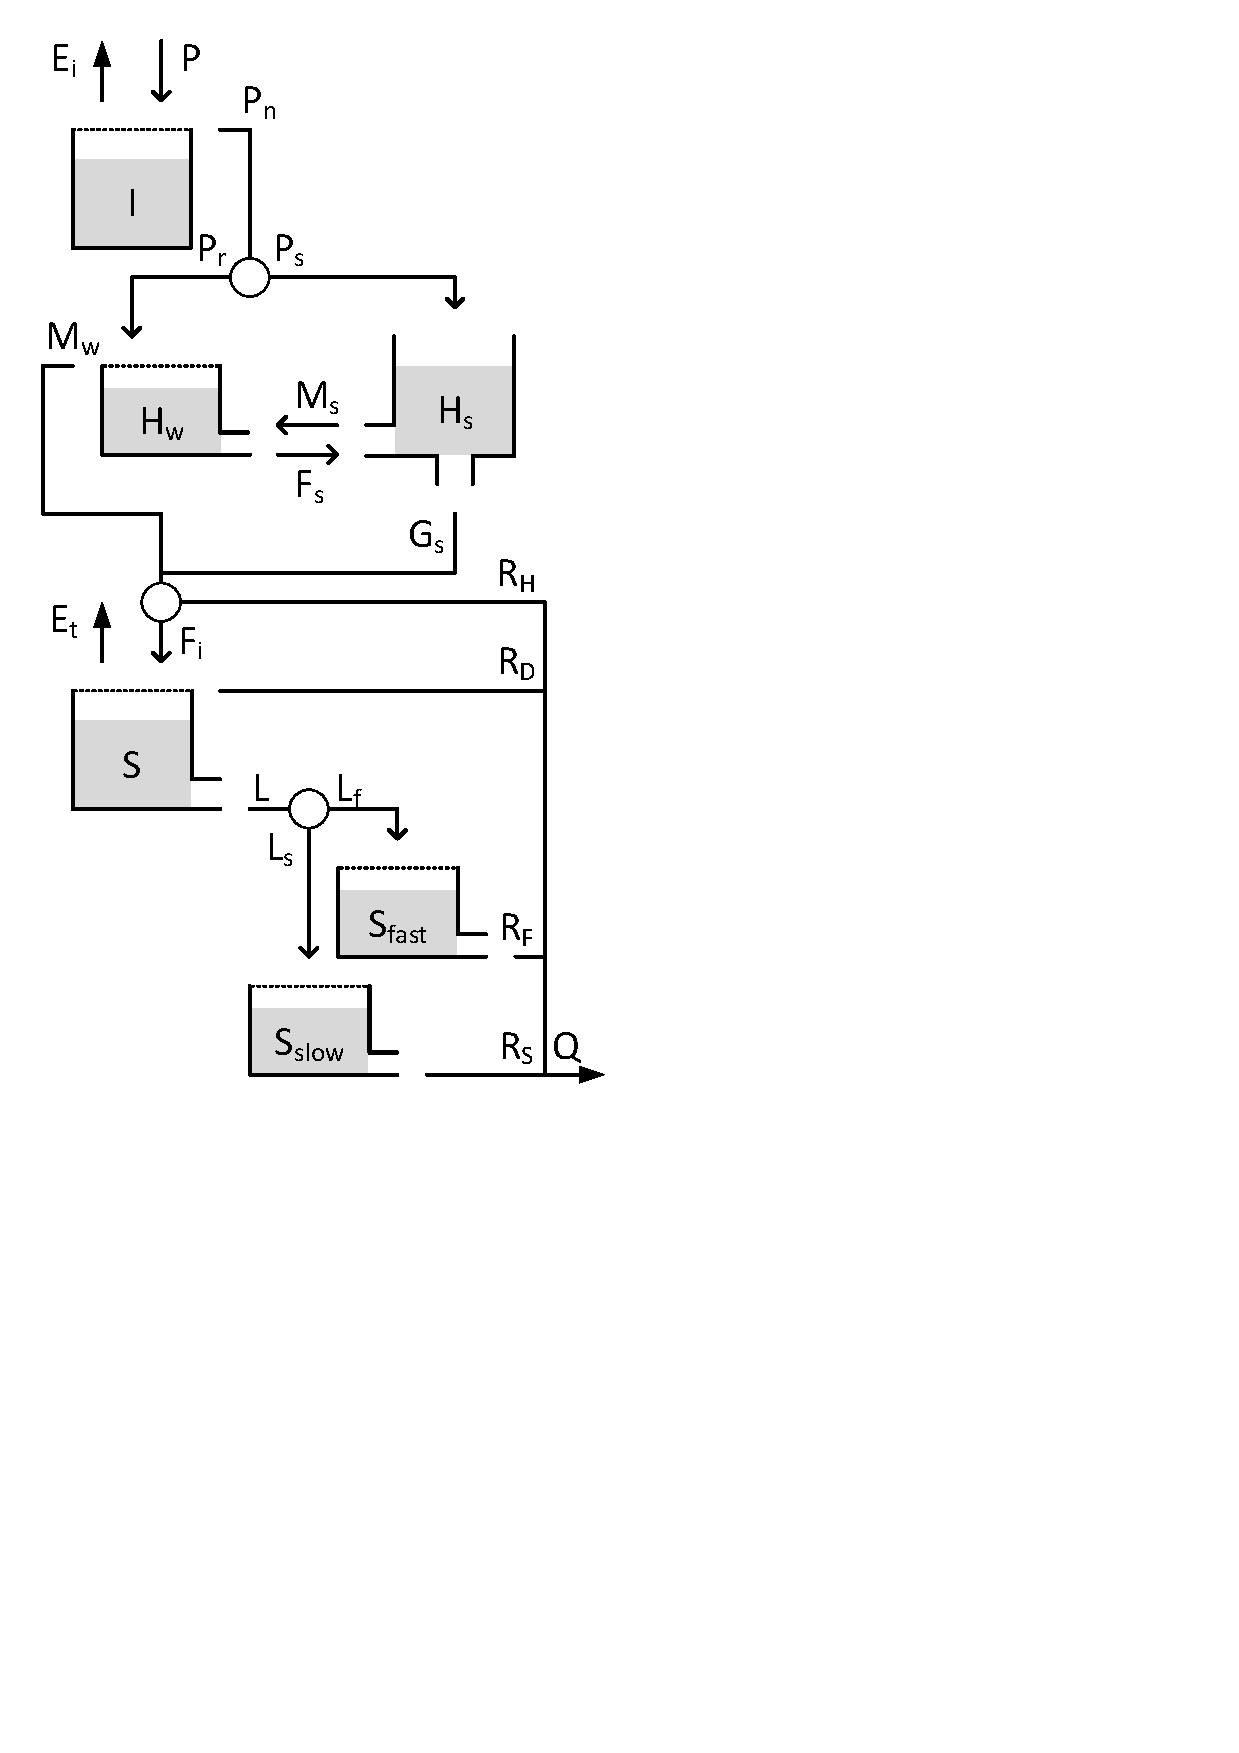
\includegraphics[trim=1cm 11cm 7cm 1cm,width=7cm,keepaspectratio]{./AppA_files/44_schematic.pdf}
\caption{Structure of the ECHO model} \label{fig:44_schematic}
\end{wrapfigure}

\begin{align}
	\frac{dI}{dt} &= P-E_i-P_n \\
	E_i &= \begin{cases}
		E_p, &\text{if } I >0 \\
		0, & \text{otherwise} \\
	\end{cases} \\
	P_n &= 
	\begin{cases}
		P, & \text{if } I = \rho \\
		0, & \text{otherwise}
	\end{cases}
\end{align}

Where $I$ [mm] is the current interception storage, refilled by precipitation $P$ $[mm/d]$ and drained by evaporation $E_i$ $[mm/d]$ and net precipitation $P_n$ $[mm/d]$.
$E_i$ occurs at the potential rate $E_p$ $[mm/d]$ when possible. 
$P_n$ only occurs when the store is at maximum capacity $\rho$ [mm].

} % end of wrapfigure fix

\begin{align}
	\frac{dH_s}{dt} &= P_s + F_s - M_s - G_s\\
	P_s &= \begin{cases}
		P_n, &\text{if } T \leq T_s \\
		0, & \text{otherwise} \\
	\end{cases} \\
	M_s &= \begin{cases}
		a_s(T-T_m), &\text{if } T > T_m, H_s > 0 \\
		0, &\text{otherwise}\\
	\end{cases}	\\
	F_s &= \begin{cases}
		a_fa_s(T_m-T), &\text{if } T < T_m, H_w > 0 \\
		0, &\text{otherwise}\\
	\end{cases} \\
	G_s &= \begin{cases}
		G_{max}, &\text{if } H_s > 0 \\
		0, &\text{otherwise} \\
	\end{cases} 
\end{align}

Where $H_s$ [mm] is the current storage in the snow pack, refilled by precipitation-as-snow $P_s$ $[mm/d]$ and refreezing of melted snow $F_s$ $[mm/d]$, and drained by snowmelt $M_s$ $[mm/d]$ and the ground-heat flux $G_s$ $[mm/d]$.
$P_s$ is calculated as all effective rainfall after interception, provided the temperature is below a threshold $T_s$ $[^oC]$.
$M_s$ uses a degree-day factor $a_s$ $[mm/^oC/d]$ and threshold temperature for snowmelt $T_m$ $[^oC]$.
$F_s$ occurs if the current temperature is below $T_m$ and the degree-day rate reduced by factor $a_f$ [-].
$G_s$ occurs at a constant rate $G_{max}$ $[mm/d]$.

\begin{align}
	\frac{dH_w}{dt} &= P_r +M_s-F_s-M_w \\
	P_r &= \begin{cases}
		P_n, &\text{if } T > T_s \\
		0, & \text{otherwise} \\
	\end{cases} \\
	M_w &=\begin{cases}
		P_r + M_s, &\text{if } H_w = \theta*H_s \\
		0, & \text{otherwise} \\
	\end{cases} 
\end{align}
  
Where $H_w$ [mm] is the current storage of liquid water in the snow pack, refilled by precipitation-as-rain $P_r$ $[mm/d]$ and snowmelt $M_s$ $[mm/d]$, and drained by refreezing $F_s$ $[mm/d]$ and outflow of melt water $M_w$ $[mm/d]$.
$P_r$ is calculated as all effective rainfall after interception, provided the temperature is above a threshold $T_s$ $[^oC]$.
$M_w$ occurs only if the store is at maximum capacity, which is a fraction $\theta$ [-] of the current snow pack height $H_s$ [mm].

\begin{align}
	\frac{dS}{dt} &= F_i - R_D -E_t -L \\
	F_i &= P_{eq} - R_H\\
	P_{eq} &= M_w+G_s\\
	R_H &= \begin{cases}
		max(P_{eq}-\phi,0), &\text{if } S < S_{max} \\
		0, & \text{otherwise} \\
	\end{cases} \\
	R_D &= \begin{cases}
		P_{eq}, &\text{if } S = S_{max} \\
		0, & \text{otherwise} \\
	\end{cases} \\
	E_t &= min\left(max\left(0,E_{t,pot}\frac{S-sw}{sm -sw}\right), E_{t,pot}\right)\\
	E_{t,pot} &= E_p - E_i\\
	L &= K_{sat}S^c
\end{align}

Where $S$ [mm] is the current storage in the soil moisture zone, refilled by infiltration $F_i$ $[mm/d]$ and drained by Dunne-type runoff $R_D$ $[mm/d]$, evapotranspiration $E_t$ $[mm/d]$ and leakage $L$ $[mm/d]$.
$F_i$ is calculated as equivalent precipitation $P_{eq}$ minus Horton-type runoff $R_H$. 
$P_{eq}$ is the sum of melt water $M_w$ and the ground-heat flux $G_s$. 
$R_H$ occurs at fixed rate $\phi$ $[mm/d]$ and only if the soil moisture is not saturated.
$R_D$ is equal to equivalent precipitation $P_{eq}$ but occurs only when the store is at maximum capacity $S_{max}$ [mm].
$E_t$ fulfils any leftover evaporation demand after interception. 
$ E_t$ occurs at the potential rate until the plant stress point $sm$ [mm], decreases linearly until the wilting point $sw$ [mm] and is zero for any lower storage values.
$L$ has a non-linear relationship with storage through time parameter $K_{sat}$ $[d^{-1}]$ and coefficient $c$ [-].

\begin{align}
	\frac{S_{fast}}{dt} &= L_f - R_f\\
	L_f &= L-L_{s} \\
	L_s &= min(L,L_{max}) \\
	R_f &= k_f * S_{fast} 
\end{align}

Where $S_{fast}$ [mm] is the current storage in the fast runoff reservoir, refilled by leakage-to-fast-flow $L_f$ $[mm/d]$ and drained by fast runoff $R_f$ $[mm/d]$.
$L_f$ depends on leakage $L$ from soil moisture and the leakage-to-slow-flow $L_s$. 
$L_s$ is calculated from a maximum leakage rate $L_{max}$ $[mm/d]$.
$R_f$ has a linear relation with storage through time parameter $k_f$ $[mm/d]$.

\begin{align}
	\frac{dS_{slow}}{dt} &= L_s - R_s \\
	R_s &= k_s * S_{slow} 
\end{align}

Where $S_{slow}$ [mm] is the current storage in the slow runoff reservoir, refilled by leakage-to-slow-flow $L_s$ $[mm/d]$ and drained by slow runoff $R_s$ $[mm/d]$.
$R_s$ has a linear relation with storage through time parameter $k_s$ $[mm/d]$.
Total flow:

\begin{align}
	Q &= R_H+R_D+R_F+R_S
\end{align}

\subsection{Parameter overview}
% Table generated by Excel2LaTeX from sheet 'Sheet1'
\begin{table}[htbp]
  \centering
    \begin{tabular}{lll}
    \toprule
    Parameter & Unit  & Description \\
    \midrule
    $\rho$ & $mm$  & Maximum interception storage \\
    $T_s$ & $^oC$ & Threshold temperature for snowfall \\
    $T_m$ & $^oC$ & Threshold temperature for snowmelt \\
    $a_s$ & $mm~^oC^{-1}~d^{-1}$ & Degree-day factor for snowmelt \\
    $a_f$ & $-$   & Degree-day factor reduction factor for refreezing \\
    $G_{max}$ & $mm~d^{-1}$ & Snow melt through ground heat flux rate \\
    $\theta$ & $-$   & Water holding capacity as fraction of current snow pack \\
    $\phi$ & $mm~d^{-1}$ & Maximum Horton type flow rate \\
    $S_{max}$ & $mm$  & Maximum soil moisture storage \\
    $sw$  & $mm$  & Wilting point \\
    $sm$  & $mm$  & Plant stress point \\
    $K_{sat}$ & $d^{-1}$ & Runoff coefficient \\
    $c$   & $-$   & Runoff non-linearity \\
    $L_{max}$ & $mm~d^{-1}$ & Maximum leakage rate \\
    $k_f$ & $d^{-1}$ & Runoff coefficient \\
    $k_s$ & $d^{-1}$ & Runoff coefficient \\
    \bottomrule
    \end{tabular}%
  \label{tab:addlabel}%
\end{table}%


\subsection{Precipitation-Runoff Modelling System (PRMS) (model ID: 45)}
The PRMS model (fig.~\ref{fig:45_schematic}) is a modelling system that, in its most recent version, allows the user to specify a wide variety of catchment processes and flux equations \citep{Markstrom2015}. The version presented here is a simplified version of the original PRMS model \citep{Leavesley1983}. Simplifications involve the use of PET time series instead of within-model estimates based on temperature, and simpler interception and snow routines. The model has 7 stores and 18 parameters ($TT$, $ddf$, $\alpha$, $\beta$, $STOR$, $RETIP$, $SCN$, $SCX$, $REMX$, $SMAX$, $c_{gw}$, $RESMAX$, $k_1$, $k_2$, $k_3$, $k_4$, $k_5$ and $k_6$). The model aims to represent:

\begin{itemizecompact}
\item Snow accumulation and melt;
\item Interception by vegetation;
\item Depression storage and impervious surface areas;
\item Direct runoff based on catchment saturation;
\item Infiltration into soil moisture and connection with deeper groundwater;
\item Potentially non-linear interflow, baseflow and groundwater sink.
\end{itemizecompact}

\subsubsection{File names}
\begin{tabular}{@{}ll}
Model: &m\_45\_prms\_18p\_7s \\
Parameter ranges: &m\_45\_prms\_18p\_7s\_parameter\_ ranges \\
\end{tabular}

% Equations
\subsubsection{Model equations}

% Model layout figure
{ 																	% This ensures it doesn't warp text further down
\begin{wrapfigure}{l}{6cm}
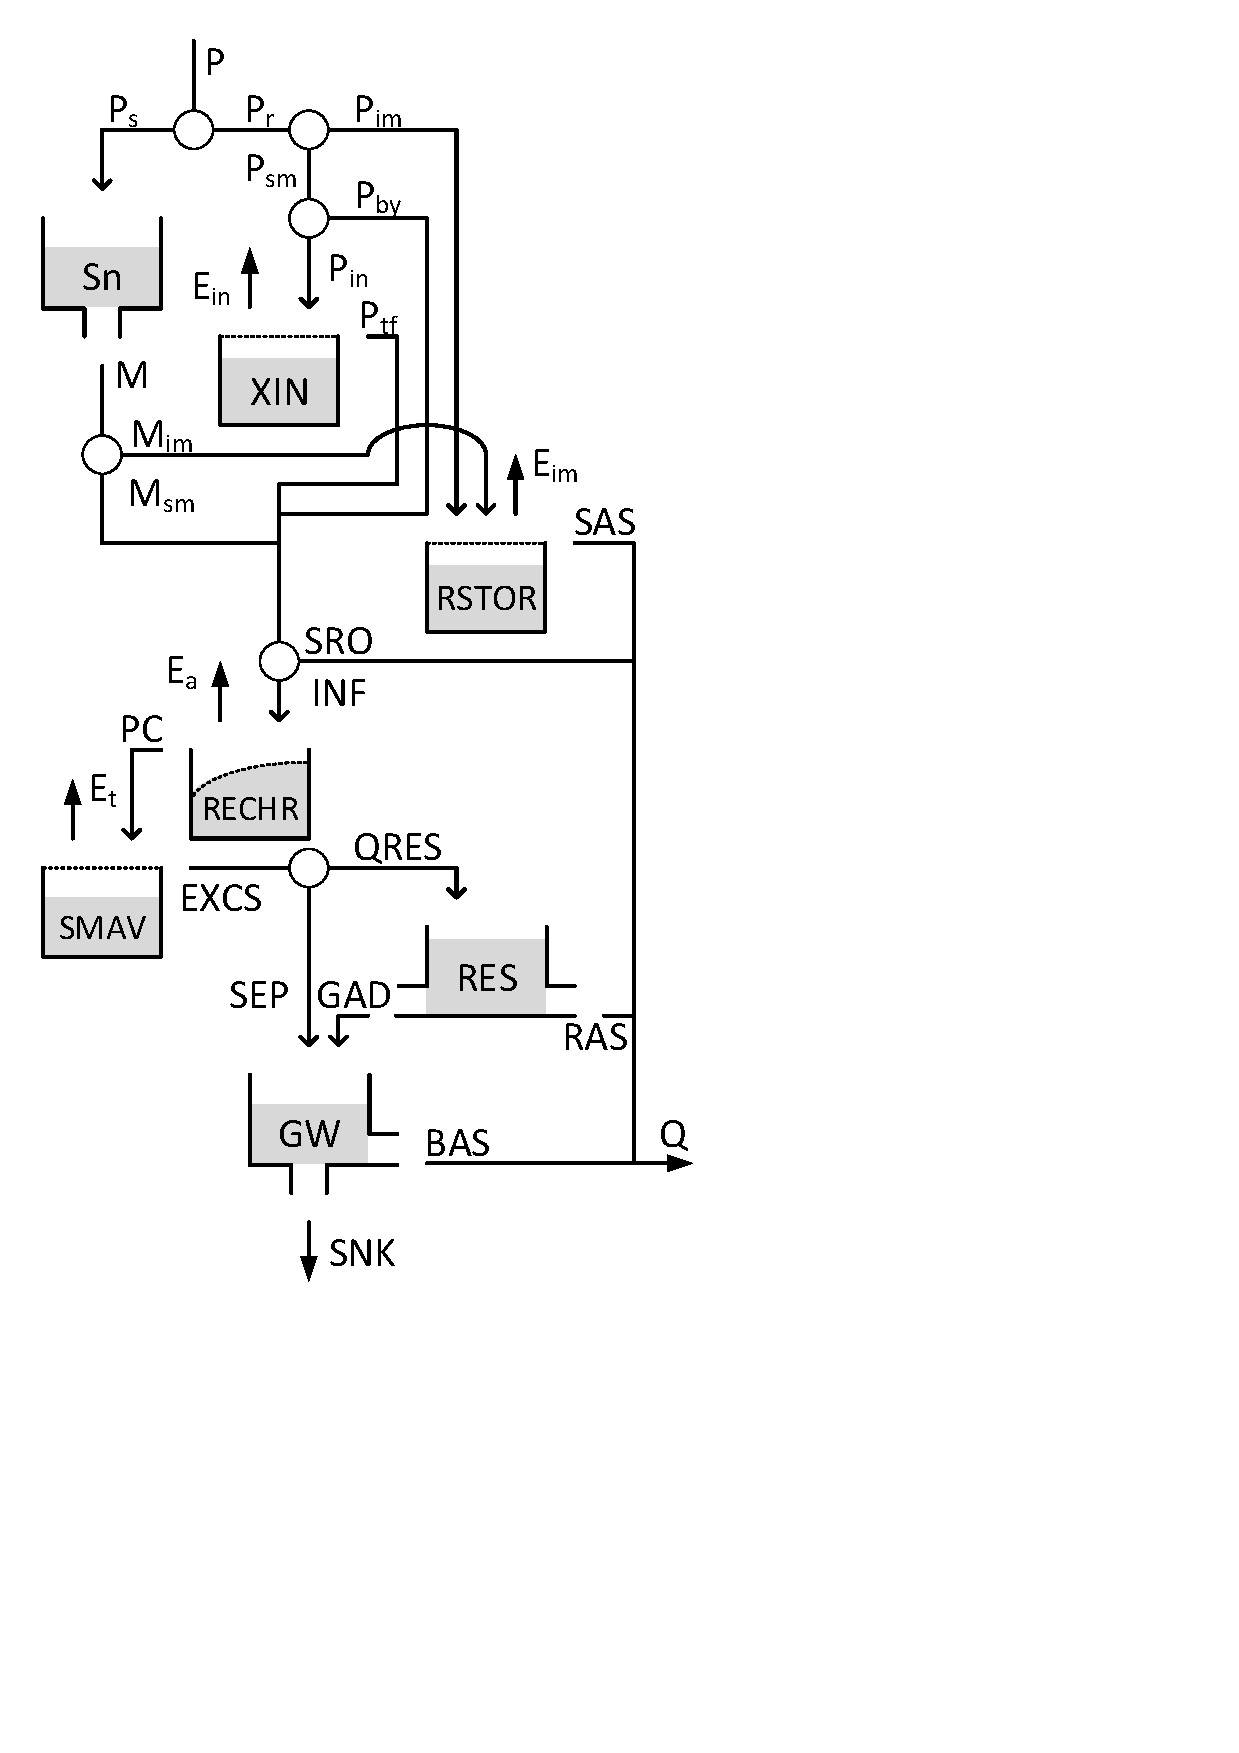
\includegraphics[trim=1cm 8cm 7cm 1cm,width=7cm,keepaspectratio]{./files/45_schematic.pdf}
\caption{Structure of the PRMS model} \label{fig:45_schematic}
\end{wrapfigure}

\begin{align}
	\frac{dSn}{dt} &= P_s-M \\
	P_s &= \begin{cases}
		P, &\text{if } T \leq TT \\
		0, & \text{otherwise} \\
	\end{cases} \\
	M &= 
	\begin{cases}
		ddf*(T - TT), & \text{if } T \geq TT \\
		0, & \text{otherwise}
	\end{cases}
\end{align}

Where S is the current snow storage [mm], $P_s$ the rain that falls as snow [mm], M the snowmelt [mm] based on a degree-day factor (ddf, [mm/\degree C/d]) and threshold temperature for snowfall and snowmelt (TT, [\degree C]).

} % end of wrapfigure fix

\begin{align}
	\frac{dXIN}{dt} &= P_{in} - E_{in} - P_{tf}\\
	P_{in} &= \alpha*P_{sm} \\
	P_{sm} &= \beta*P_r\\
	P_r &= \begin{cases}
		P, &\text{if } T > TT \\
		0, & \text{otherwise} \\
	\end{cases} \\
	E_{in} &= \begin{cases}
		\beta*E_p, & \text{if } XIN > 0 \\
		0, & \text{otherwise} \\
	\end{cases} \\
	P_{tf} &= \begin{cases}
		P_{in}, & \text{if } XIN = STOR \\
		0, & \text{otherwise}
	\end{cases}
\end{align}


Where $XIN$ [mm] is the current storage in the interception reservoir, recharged by intercepted rainfall $P_{in}$ $[mm/d]$ and drained by evaporation $E_i$ $[mm/d]$ and throughfall $P_{tf}$ $[mm/d]$. 
$P_{in}$ $[mm/d]$ is the fraction $\alpha$ [-] of rainfall on non-impervious area $P_{sm}$ $[mm/d]$ that does not bypass the interception reservoir. 
$P_{sm}$ $[mm/d]$ is the fraction $\beta$ [-] of rainfall $P_r$ $[mm/d]$ that does not fall on impervious area. 
Rainfall is given as all precipitation $P$ $[mm/d]$ that occurs when temperature $T$ [\degree C] is above a threshold $TT$ [\degree C]. 
$E_i$ $[mm/d]$ occurs at the potential rate $E_p$, corrected for the fraction of the catchment where interception can occur.
Throughfall $P_{tf}$ is all rainfall that reaches the interception reservoir when it is at maximum capacity $STOR$ [mm].

\begin{align}
	\frac{dRSTOR}{dt} &= P_{im} + M_{im} - E_{im} - SAS \\
	P_{im} &= (1-\beta)*P_r \\
	M_{im} &= (1-\beta)*M \\
	E_{im} &= \begin{cases}
		(1-\beta)*E_p, &\text{if } RSTOR > 0 \\
		0, &\text{otherwise} \\
	\end{cases} \\
	SAS &= \begin{cases}
		P_{im} +M_{im}, &\text{if } RSTOR = RETIP \\
		0, &\text{otherwise}
	\end{cases}
\end{align}

Where $RSTOR$ [mm] is current depression storage, refilled by rainfall and snowmelt on impervious area, $P_{im}$ $[mm/d]$ and $M_{im}$ $[mm/d]$ respectively, and drained by evaporation $E_{im}$  $[mm/d]$ and surface runoff $SAS$ $[mm/d]$. 
$P_{im}$ is given as the fraction $1-\beta$ of rainfall $P_r$. 
$M_{im}$ is given as the fraction $1-\beta$ of snowmelt $M$.
$E_{im}$ occurs at the potential rate $E_p$, corrected for the fraction of the catchment where impervious areas can occur.
$SAS$ occurs when the depression store is at maximum capacity $RETIP$ [mm].

\begin{align}
	\frac{dRECHR}{dt} &= INF - E_a - PC \\
	INF &= M_{sm} + P_{tf} + P_{by} - SRO\\
	M_{sm} &= \beta*M \\
	P_{by} &= (1-\alpha)*P_{sm}\\
	SRO &= \left[SCN+(SCX-SCN)*\frac{RECHR}{REMX}\right]*\left(M_{sm}+P_{tf} + P_{by}\right) \\
	E_a &= \frac{RECHR}{REMX}*\left(E_p-E_i-E_{im}\right)\\
	PC &= \begin{cases} 
		INF, &\text{if } RECHR = REMX \\
		0, &\text{otherwise}
	\end{cases}
\end{align}

Where $RECHR$ [mm] is the current storage in the upper soil moisture zone, recharged by infiltration $INF$ $[mm/d]$ and drained by evaporation $E_a$ $[mm/d]$ and percolation $PC$ $[mm/d]$.
$INF$ is the difference between incoming snowmelt $M_{sm}$ $[mm/d]$, throughfall $P_{tf}$ $[mm/d]$ and interception bypass $P_{by}$ $[mm/d]$, and surface runoff from saturated area $SRO$ $[mm/d]$. 
$S_{sm}$ is snowmelt from the fraction $\beta$ [-] of the catchment that is not impervious. 
$P_{by}$ is the fraction $1-\alpha$ of rainfall over non-impervious area $P_{sm}$ that bypasses the interception store.
$SRO$ has a linear relation between minimum contributing area $SCN$ [-] and maximum contributing area $SCX$ [-] based on current storage $RECHR$ and maximum storage $REMX$ [mm].
$E_a$ uses a similar linear relationship and accounts for already fulfilled evaporation demand by interception and impervious areas.
$PC$ occurs when the store reaches maximum capacity.

\begin{align}
	\frac{dSMAV}{dt} &= PC-E_t-EXCS\\
	E_t &=  \begin{cases} 
		\frac{SMAV}{SMAX}*\left(E_p-E_{in}-E_{im}-E_a\right), &\text{if } RECHR < \left(E_p-E_{in}-E_{im}\right)\\
		0, &\text{otherwise}\\
	\end{cases} \\
	EXCS &= \begin{cases} 
		PC, &\text{if } SMAV = SMAX-REMX \\
		0, &\text{otherwise}
	\end{cases}
\end{align}

Where $SMAV$ [mm] is the current storage in the lower soil moisture zone, recharged by percolation from the upper zone $PC$ $[mm/d]$ and drained by transpiration $E_t$ $[mm/d]$ and soil moisture excess $EXCS$ $[mm/d]$.
$E_t$ is corrected for already fulfilled evaporation demand and only occurs if the upper zone can not satisfy this demand. 
$E_t$ uses a linear relationship between current storage and the maximum storage in the lower zone $SMAX-REMX$ [mm].
$EXCS$ only occurs when the store has reached maximum capacity $SMAX-REMX$.

\begin{align}
	\frac{dRES}{dt} &= QRES-GAD-RAS\\
	QRES &= min(EXCS-SEP,0) \\
	GAD &= k_1\left(\frac{RES}{RESMAX}\right)^{k_2}\\
	RAS &= k_3*RES+k_4*RES^2\\
\end{align}

Where $RES$ [mm] is the current storage in the runoff reservoir, filled by the difference between soil moisture excess $EXCS$  $[mm/d]$ and constant groundwater recharge $SEP$  $[mm/d]$, and drained by groundwater drainage $GAD$  $[mm/d]$ and interflow component $RAS$  $[mm/d]$. 
$GAD$ is potentially non-linear using time coefficient $k_1$ $[d^{-1}]$ and non-linearity coefficient $k_2$ [-], and is also scaled by the maximum reservoir capacity $RESMAX$ [mm]. 
$RAS$ is non-linear interflow based on coefficients $k_3$ $[d^{-1}]$ and $k_4$ $[mm^{-1}d^{-1}]$.

\begin{align}
	\frac{dGW}{dt} &= SEP+GAD-BAS-SNK\\
	SEP &= min(c_{gw},EXCS) \\
	BAS &= k_5*GW\\
	SNK &= k_6*GW
\end{align}

Where $GW$ [mm] is the current groundwater storage, refilled by groundwater recharge from soil moisture $SEP$ and recharge from runoff reservoir $GAD$ and drained by baseflow $BAS$  $[mm/d]$ and flow to deeper groundwater $SNK$  $[mm/d]$.
$SEP$ occurs at the maximum rate $c_{gw}$ $[mm/d]$ if possible.
$BAS$ is a linear reservoir with time coefficient $k_5$  $[d^{-1}]$.
$SNK$ is a linear reservoir with time coefficient $k_6$ $[d^{-1}]$.
Total flow $Q_t$  $[mm/d]$:

\begin{align}
	Q_t &= SAS+SRO+RAS+BAS
\end{align}

\newpage
\subsubsection{Parameter overview}
% Table generated by Excel2LaTeX from sheet 'Sheet1'
\begin{table}[htbp]
  \centering
    \begin{tabular}{lll}
    \toprule
    Parameter & Unit  & Description \\
    \midrule
    $TT$  & $^oC$ & Threshold temperature for snowfall and snowmelt \\
    $ddf$ & $mm~^oC^{-1}~d^{-1}$ & Degree-day factor for snowmelt \\
    $\alpha$ & $-$   & Fraction of precipitation on soil that is intercepted \\
    $\beta$ & $-$   & Fraction of precipitation that falls on soil \\
    $STOR$ & $mm$  & Maximum interception storage \\
    $RETIP$ & $mm$  & Maximum depression storage \\
    $SCN$ & $-$   & Minimum contributing area to surface runoff \\
    $SCX$ & $-$   & Maximum contributing area to surface runoff \\
    $REMX$ & $mm$  & Maximum upper soil moisture storage \\
    $SMAX$ & $mm$  & Maximum total soil moisture storage \\
    $c_{gw}$ & $mm~d^{-1}$ & Maximum groundwater recharge rate \\
    $RESMAX$ & $mm$  & Maximum runoff routing storage \\
    $k_1$ & $d^{-1}$ & Runoff coefficient \\
    $k_2$ & $-$   & Runoff non-linearity \\
    $k_3$ & $d^{-1}$ & Runoff coefficient \\
    $k_4$ & $mm^{-1}~d^{-1}$ & Runoff coefficient \\
    $k_5$ & $d^{-1}$ & Runoff coefficient \\
    $k_6$ & $d^{-1}$ & Runoff coefficient \\
    \bottomrule
    \end{tabular}%
  \label{tab:addlabel}%
\end{table}%


\subsection{Climate and Land-use Scenario Simulation in Catchments model (model ID: 46)}
The CLASSIC model (fig.~\ref{fig:46_schematic}) is developed as a modular semi-distributed grid-based rainfall runoff model \citep{Crooks2007}. For comparability with other models the grid-based routing component is not included here, nor is the arable soil element because input data for this soil type is not supported. The model represents runoff from three different soil categories: permeable, semi-permeable and impermeable. It has 8 stores and 12 parameters ($f_{ap}$, $f_{dp}$, $d_p$, $c_q$, $d_1$, $f_{as}$, $f_{ds}$, $d_s$, $d_2$, $c_{xq}$, $c_{xs}$ and $c_{u}$). The model aims to represent:

\begin{itemizecompact}
\item Division into permeable, semi-permeable and impermeable areas;
\item Infiltration into permeable soils and deficit-based soil moisture accounting;
\item Infiltration into semi-permeable soils and direct runoff from semi-permeable soils (bypassing the moisture accounting);
\item Fixed interception on impermeable soils;
\item Linear flow routing from permeable soils;
\item Fast and slow routing from semi-permeable soils;
\item Linear flow routing from impermeable soils.
\end{itemizecompact}

\subsubsection{File names}
\begin{tabular}{@{}ll}
Model: &m\_46\_classic\_12p\_8s \\
Parameter ranges: &m\_46\_classic\_12p\_8s\_parameter\_ ranges \\
\end{tabular}

% Equations
\subsubsection{Model equations}

% Model layout figure
{ 																	% This ensures it doesn't warp text further down
\begin{wrapfigure}{l}{8cm}
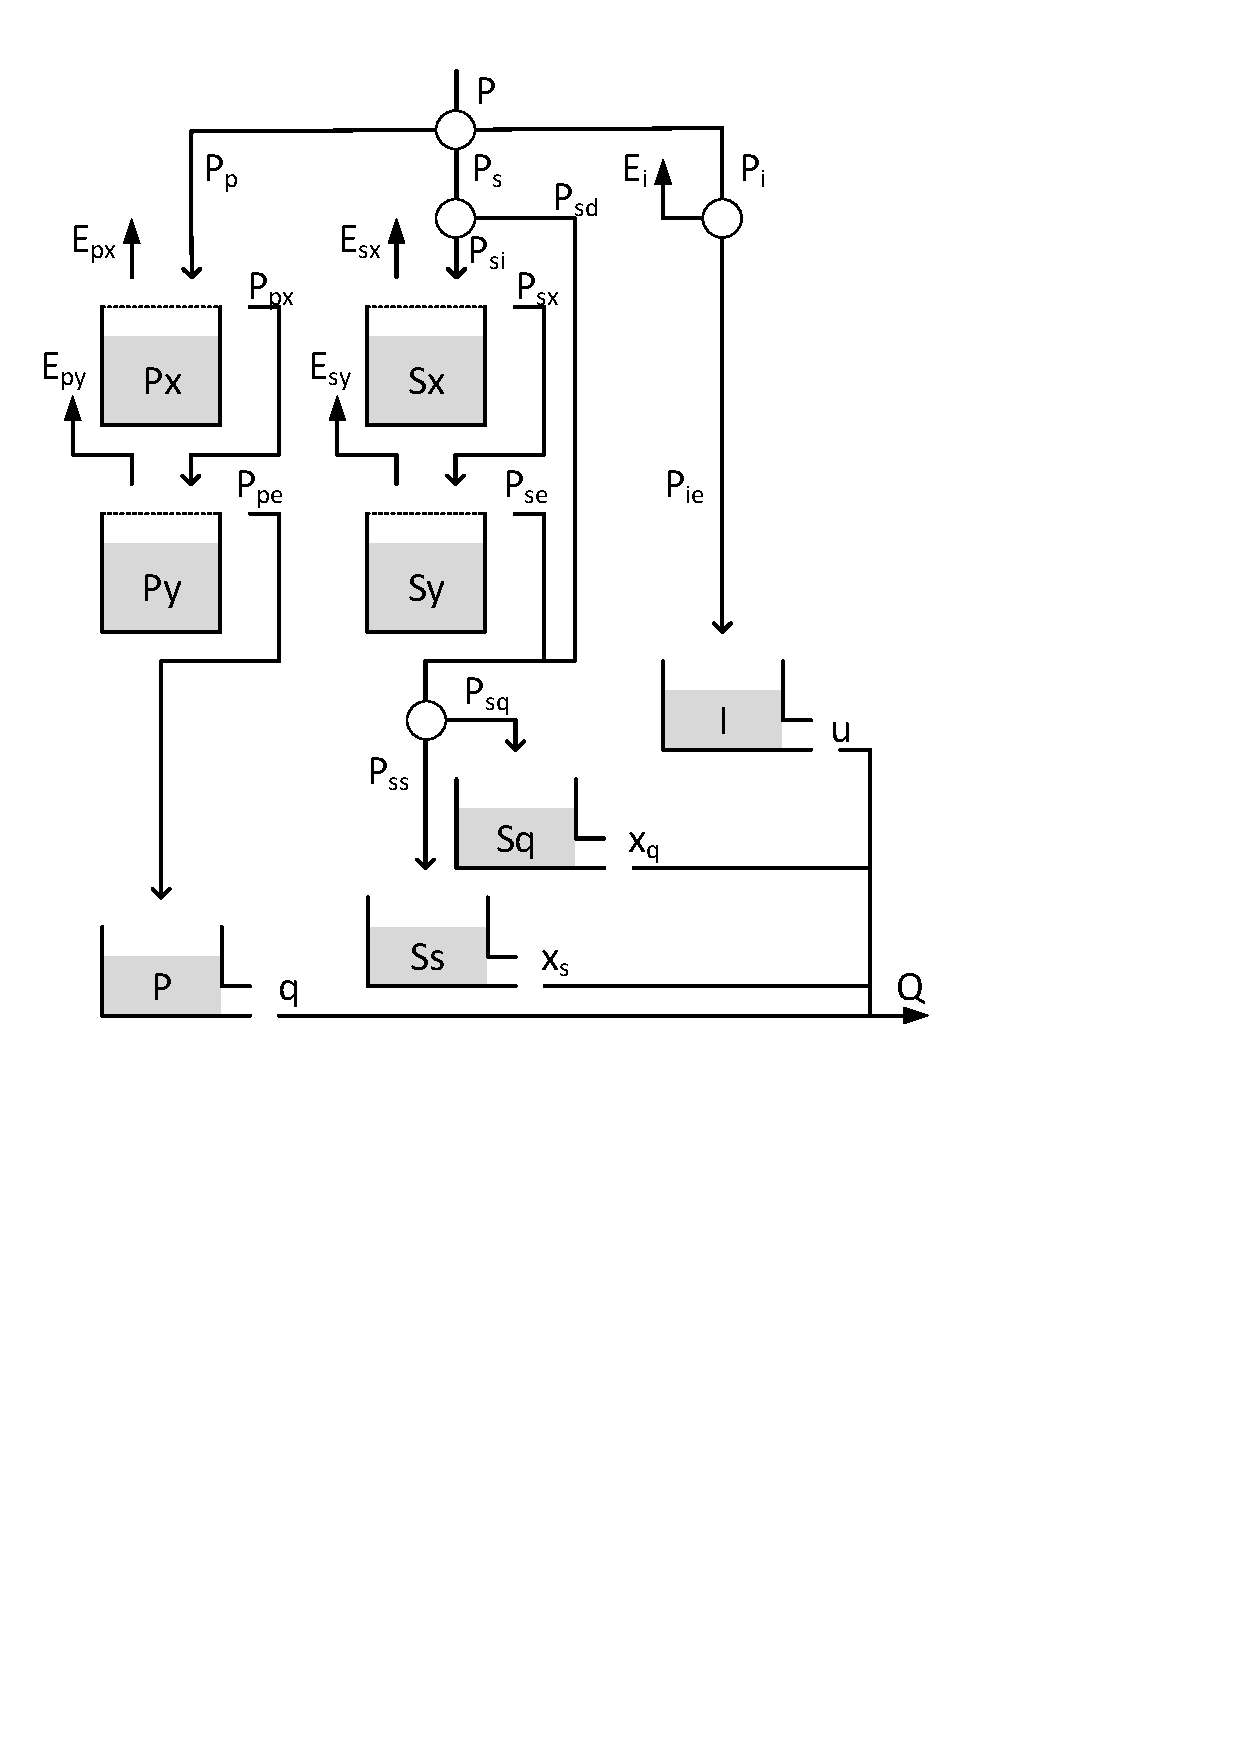
\includegraphics[trim=1cm 12cm 7cm 1cm,width=7cm,keepaspectratio]{./files/46_schematic.pdf}
\caption{Structure of the CLASSIC model} \label{fig:46_schematic}
\end{wrapfigure}

% permeable soils

\begin{align}
	\frac{dP_x}{dt} &= P_p-E_{px}-P_{px} \\
	P_p &= f_{ap} * P\\
	E_{px} &= 
	\begin{cases}
		f_{ap}*E_p, & \text{if } P_x > 0 \\
		0, & \text{otherwise}\\
	\end{cases}\\
	P_{px} &= 
	\begin{cases}
		P_p, & \text{if } P_x = f_{dp}*d_p \\
		0, & \text{otherwise}
	\end{cases}
\end{align}

Where $P_x$ [mm] is the current storage in the upper permeable layer, refilled by precipitation $P_p$ $[mm/d]$ and drained 

} % end of wrapfigure fix

\noindent 
$P_p$ is the fraction of precipitation $P$ $[mm/d]$ that falls on permeable area $f_{ap}$ [-].
$E_{px}$ occurs at the potential rate $E_p$ $[mm/d]$ whenever possible, adjusted for the fraction of area that is permeable soil.
$P_{px}$ only occurs when the store is at maximum capacity $f_{dp}*d_p$, where $d_p$ is the total soil depth (sum of depths X and Y) in the permeable area and $f_{dp}$ the fraction of this depth that is store X.

\begin{align}
	\frac{dP_y}{dt} &= -P_{px}+E_{py}+P_{pe} \\
	E_{py} &= 1.9*exp\left[{\frac{-0.6523*(P_y+f_{dp}*d_p)}{f_{dp}*d_p}}\right]*\left(f_{ap}*E_p - E_{px}\right)\\
	P_{pe} &= 
	\begin{cases}
		P_{px}, & \text{if } P_y = 0 \\
		0, & \text{otherwise}
	\end{cases}
\end{align}

Where $P_y$ [mm] is the current \emph{deficit}, which is increased by evaporation $E_{py}$ $[mm/d]$ and decreased by inflow $P_{px}$ $[mm/d]$.
Effective precipitation $P_{pe}$ $[mm/d]$ is only generated when the deficit is 0.
$E_{py}$ decreases exponentially with increasing deficit.

\begin{align}
	\frac{dP}{dt} &= P_{pe}-q \\
	q &= c_q*P
\end{align}

Where $P$ [mm] is the current storage in the permeable soil routing store, refilled by effective rainfall on permeable soil $P_{pe}$ $[mm/d]$ and drained by baseflow $q$ $[mm/d]$.
$q$ has a linear relation with storage through time scale parameter $c_p$ $[d^{-1}]$.

% semi-permeable soils
\begin{align}
	\frac{dS_x}{dt} &= P_{si}-E_{sx}-P_{sx} \\
	P_{si} &= d_1*P_s \\
	P_s &= f_{as}* P\\
	E_{sx} &= 
	\begin{cases}
		f_{as}*E_p, & \text{if } S_x > 0 \\
		0, & \text{otherwise}\\
	\end{cases}\\
	P_{sx} &= 
	\begin{cases}
		P_s, & \text{if } S_x = f_{ds}*d_s \\
		0, & \text{otherwise}
	\end{cases}
\end{align}

Where $S_x$ [mm] is the current storage in the upper semi-permeable layer, refilled by infiltration $P_{si}$ $[mm/d]$ and drained by evaporation $E_{sx}$ $[mm/d]$ and excess flow $P_{sx}$ $[mm/d]$.
$P_{si}$ is the fraction $d_1$ [-] of precipitation on semi-permeable area $P_s$ that infiltrates into the soil.
The complementary fraction $1-d_1$ of $P_s$ bypasses the soil and directly becomes effective rainfall as $P_{sd}$.
$P_s$ is the fraction of precipitation $P$ $[mm/d]$ that falls on semi-permeable area $f_{as}$ [-] .
$E_{sx}$ occurs at the potential rate $E_p$ $[mm/d]$ whenever possible, adjusted for the fraction of area that is semi-permeable soil.
$P_{sx}$ only occurs when the store is at maximum capacity $f_{ds}*d_s$, where $d_s$ is the total soil depth (sum of depths X and Y) in the semi-permeable area and $f_{ds}$ the fraction of this depth that is store X.

\begin{align}
	\frac{dS_y}{dt} &= -P_{sx}+E_{sy}+P_{se} \\
	E_{sy} &= 1.9*exp\left[{\frac{-0.6523*(S_y+f_{ds}*d_s)}{f_{ds}*d_s}}\right]*\left(f_{as}*E_p - E_{sx}\right)\\
	P_{pe} &= 
	\begin{cases}
		P_{sx}, & \text{if } S_y = 0 \\
		0, & \text{otherwise}
	\end{cases}
\end{align}

Where $S_y$ [mm] is the current \emph{deficit}, which is increased by evaporation $E_{sy}$ $[mm/d]$ and decreased by inflow $P_{sx}$ $[mm/d]$.
Effective precipitation $P_{se}$ $[mm/d]$ is only generated when the deficit is 0.
$E_{sy}$ decreases exponentially with increasing deficit.

\begin{align}
	\frac{dS_q}{dt} &= P_{sq}-x_q \\
	P_{sq} &= d_2*(P_{se}+P_{sd})\\	
	x_q &= c_{xq}*S_q
\end{align}

Where $S_q$ [mm] is the current storage in the semi-permeable quick soil routing store, refilled by a fraction of effective rainfall on semi-permeable soil $P_{sq}$ $[mm/d]$ and drained by quick flow $x_q$ $[mm/d]$.
$P_{sq}$ is the fraction $d_2$ [-] of $(P_{se}+P_{Sd})$ that is quick flow.
$x_q$ has a linear relation with storage through time scale parameter $c_{xq}$ $[d^{-1}]$.

\begin{align}
	\frac{dS_s}{dt} &= P_{ss}-x_s \\
	P_{ss} &= (1-d_2)*(P_{se}+P_{sd})\\	
	x_s &= c_{xs}*S_s
\end{align}

Where $S_s$ [mm] is the current storage in the semi-permeable quick soil routing store, refilled by a fraction of effective rainfall on semi-permeable soil $P_{ss}$ $[mm/d]$ and drained by slow flow $x_s$ $[mm/d]$.
$P_{ss}$ is the fraction $1-d_2$ [-] of $(P_{se}+P_{Sd})$ that is slow flow.
$x_s$ has a linear relation with storage through time scale parameter $c_{xs}$ $[d^{-1}]$.

%impermeable soils

\begin{align}
	\frac{dI}{dt} &= P_{ie}-u \\
	P_{ie} &= P_i-E_i\\
	P_i &= P-P_p-P_s\\
	u &= c_{u}*I
\end{align}

Where $I$ [mm] is the current storage in the impermeable soil routing store, refilled by effective rainfall on impermeable soil $P_{ie}$ $[mm/d]$ and drained by baseflow $u$ $[mm/d]$.
$P_{ie}$ is the remained of precipitation on impermeable soils $P_i$ $[mm/d]$, after a constant evaporation $E_i$ has been extracted.
$E_i$ is fixed at 0.5 $[mm/d]$.
$x_s$ has a linear relation with storage through time scale parameter $c_{xs}$ $[d^{-1}]$.
Total flow:

\begin{align}
	Q = q+x_s+x_q+u
\end{align}

\subsubsection{Parameter overview}
% Table generated by Excel2LaTeX from sheet 'Sheet1'
\begin{table}[htbp]
  \centering
    \begin{tabular}{lll}
    \toprule
    Parameter & Unit  & Description \\
    \midrule
    $f_{ap}$ & $-$   & Fraction permeable area \\
    $f_{dp}$ & $-$   & Store depth as fraction of $d_p$ \\
    $d_p$ & $mm$  & Total storage of Px and Py \\
    $c_q$ & $d^{-1}$ & Runoff coefficient \\
    $d_1$ & $-$   & Fraction of precipitation on semi-permeable area to Sx \\
    $f_{as}$ & $-$   & Fraction semi-permeable area \\
    $f_{ds}$ & $-$   & Store depth as fraction of $d_s$ \\
    $d_s$ & $mm$  & Total storage of Sx and Sy \\
    $d_2$ & $-$   & Fraction of semi-permeable area subsurface flow that is quick flow \\
    $c_{xq}$ & $d^{-1}$ & Runoff coefficient \\
    $c_{xs}$ & $d^{-1}$ & Runoff coefficient \\
    $c_{u}$ & $d^{-1}$ & Runoff coefficient \\
    \bottomrule
    \end{tabular}%
  \label{tab:addlabel}%
\end{table}%







\newpage
\section{Flux equations} 		\label{sec:flux}
Section \ref{sec:mod_desc} gives descriptions of each model and provides both Ordinary Differential Equations and the constitutive functions that describe each model's fluxes. These constitutive functions and any relevant constraints are implemented in MARRMoT as individual \emph{flux files}. Each \emph{flux file} contains computer code that combines the constitutive function and constraints (if needed). \emph{Flux files} are located in the folder ''./MARRMoT/Models/Flux files/''. The User Manual contains details on understanding, modifying and creating new \emph{flux files}. Table \ref{tab:sm2_1} shows a complete overview of fluxes currently implemented in MARRMoT.

% Place a caption
\vfill{}
\captionof{table}[Computational implementation of constitutive flux equations]{Equations from model descriptions and their implementation in MARRMoT (Table starts on following page) \label{tab:sm2_1}}


% BIIIIIIG table
%\afterpage{\clearpage}

\clearpage
\KOMAoptions{paper=A3,paper=landscape,pagesize}
\recalctypearea



%\begin{landscape}
%\pagestyle{empty} 	% remove page numbers
%\centering
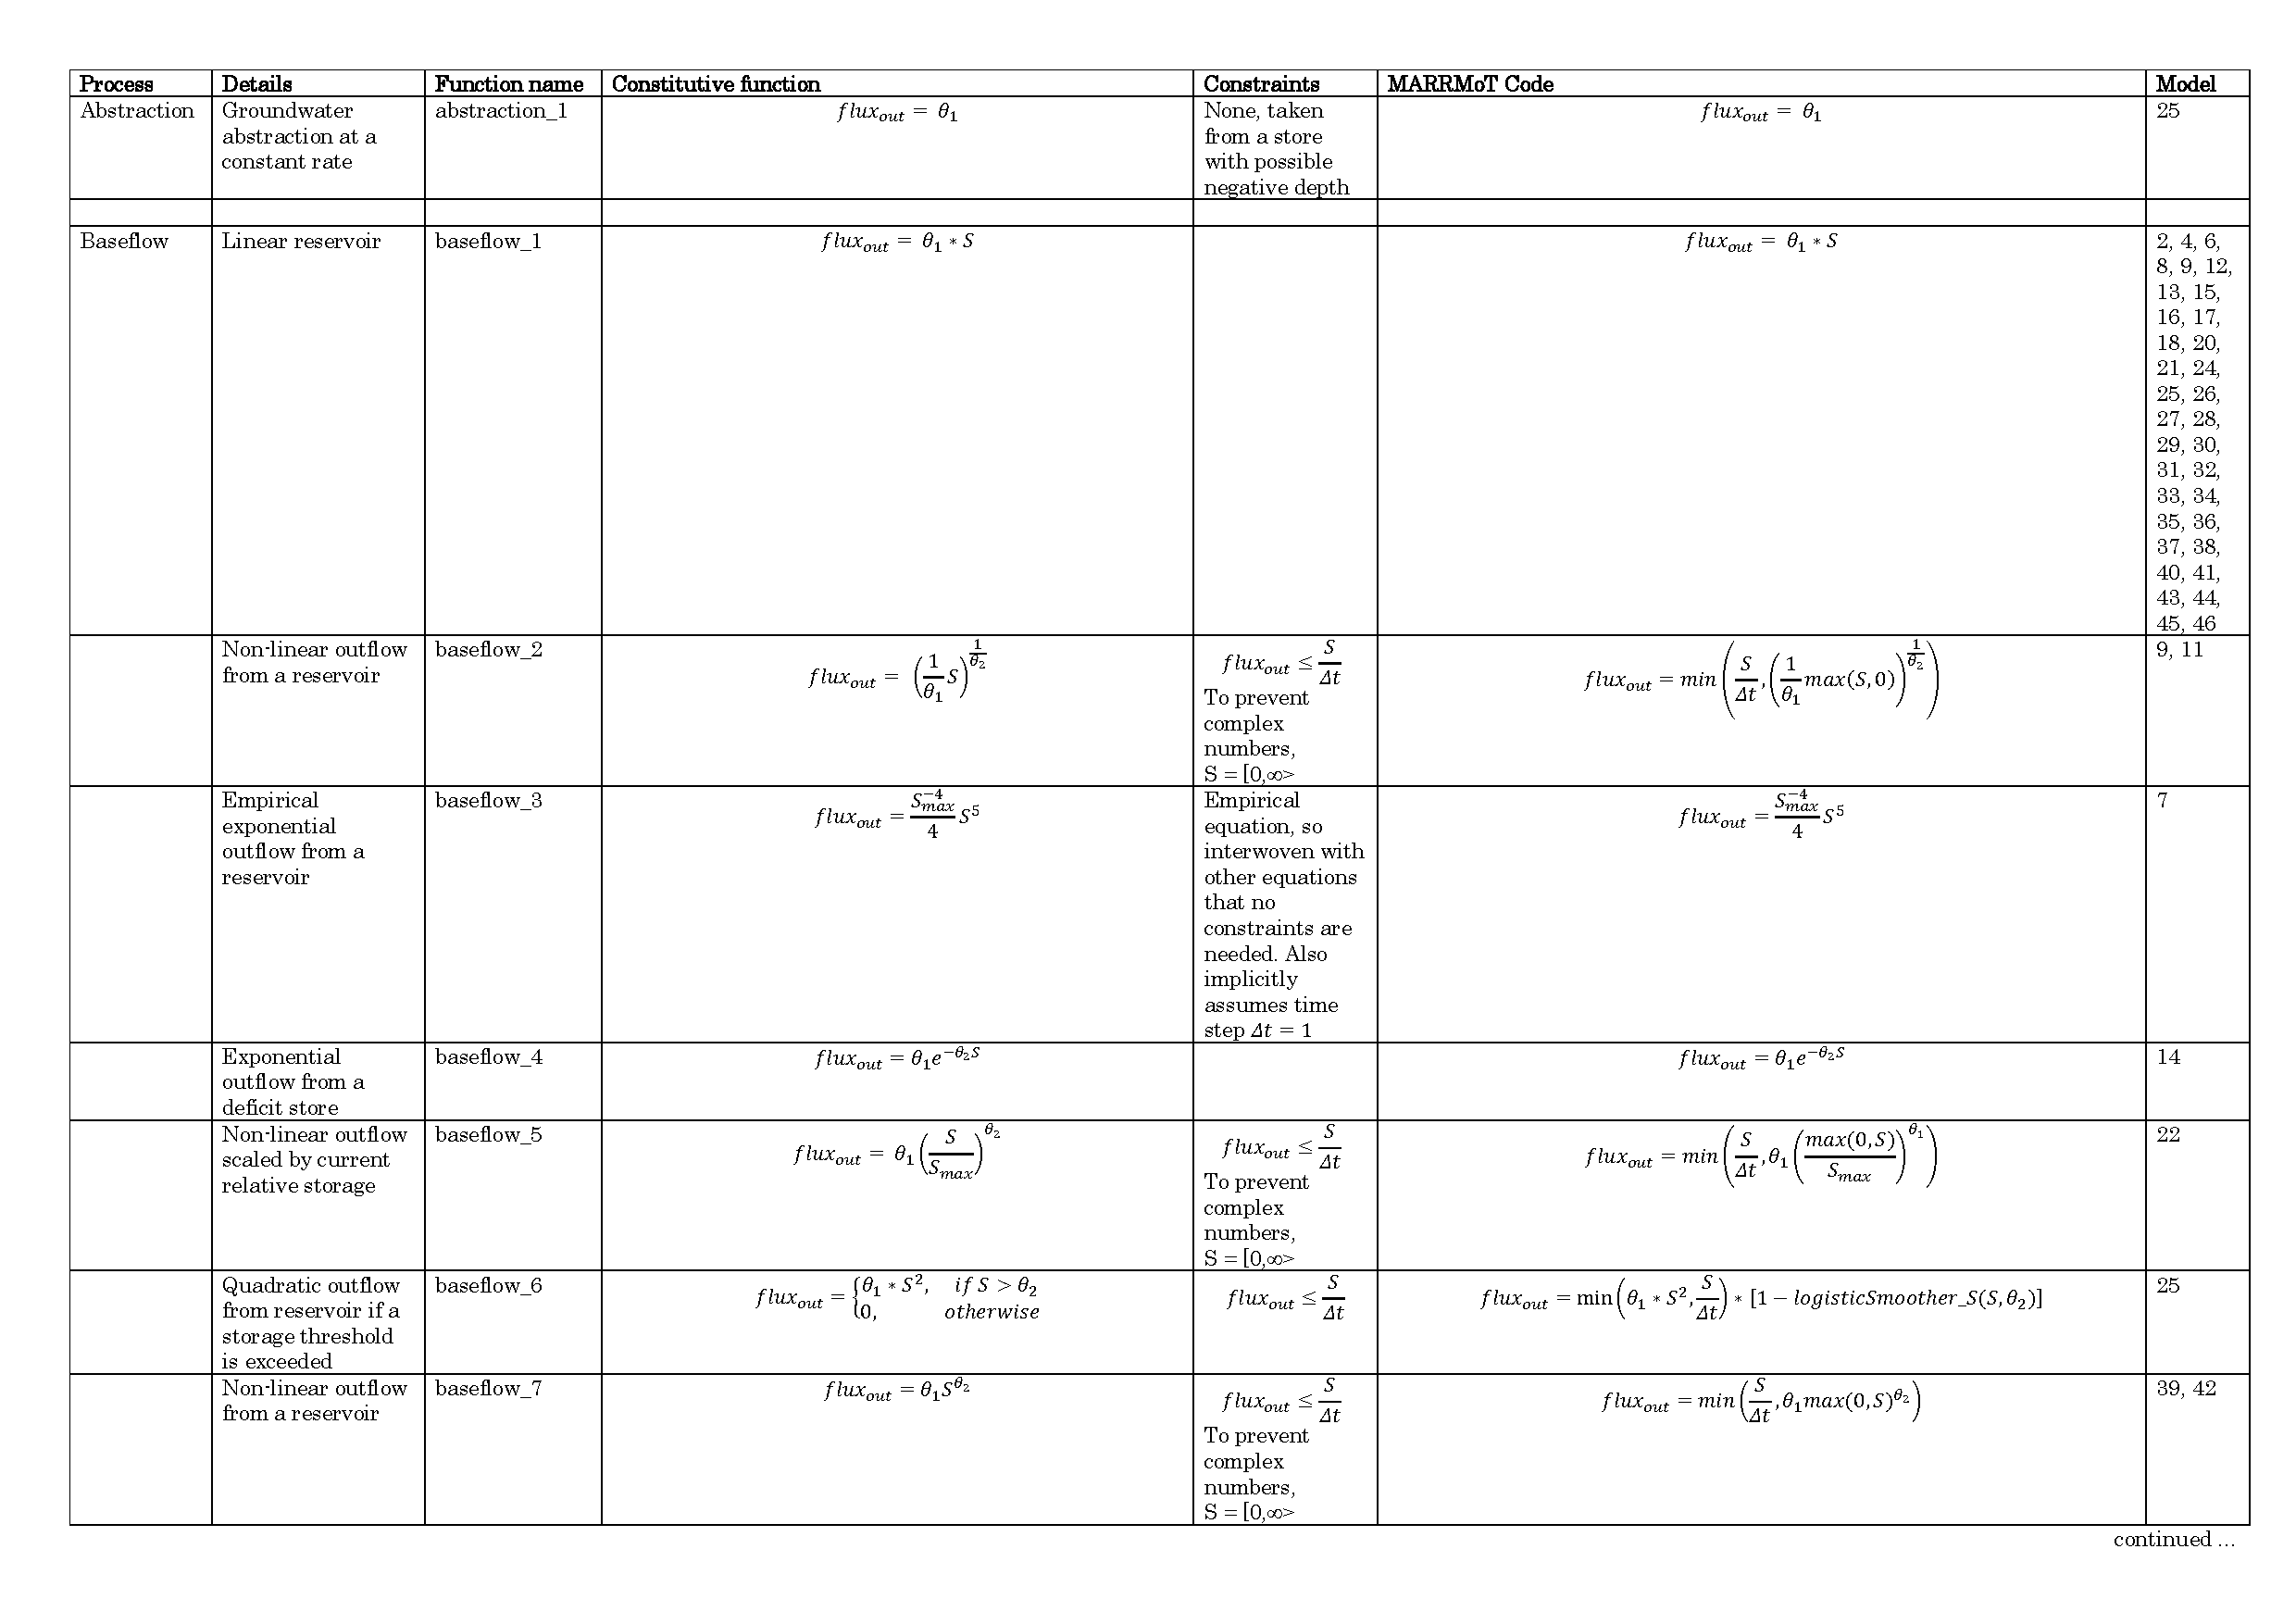
\includepdf[pages=-,pagecommand={\thispagestyle{styleLandscapeA3}}]{sm2_fluxes.pdf}
%\end{landscape}

% 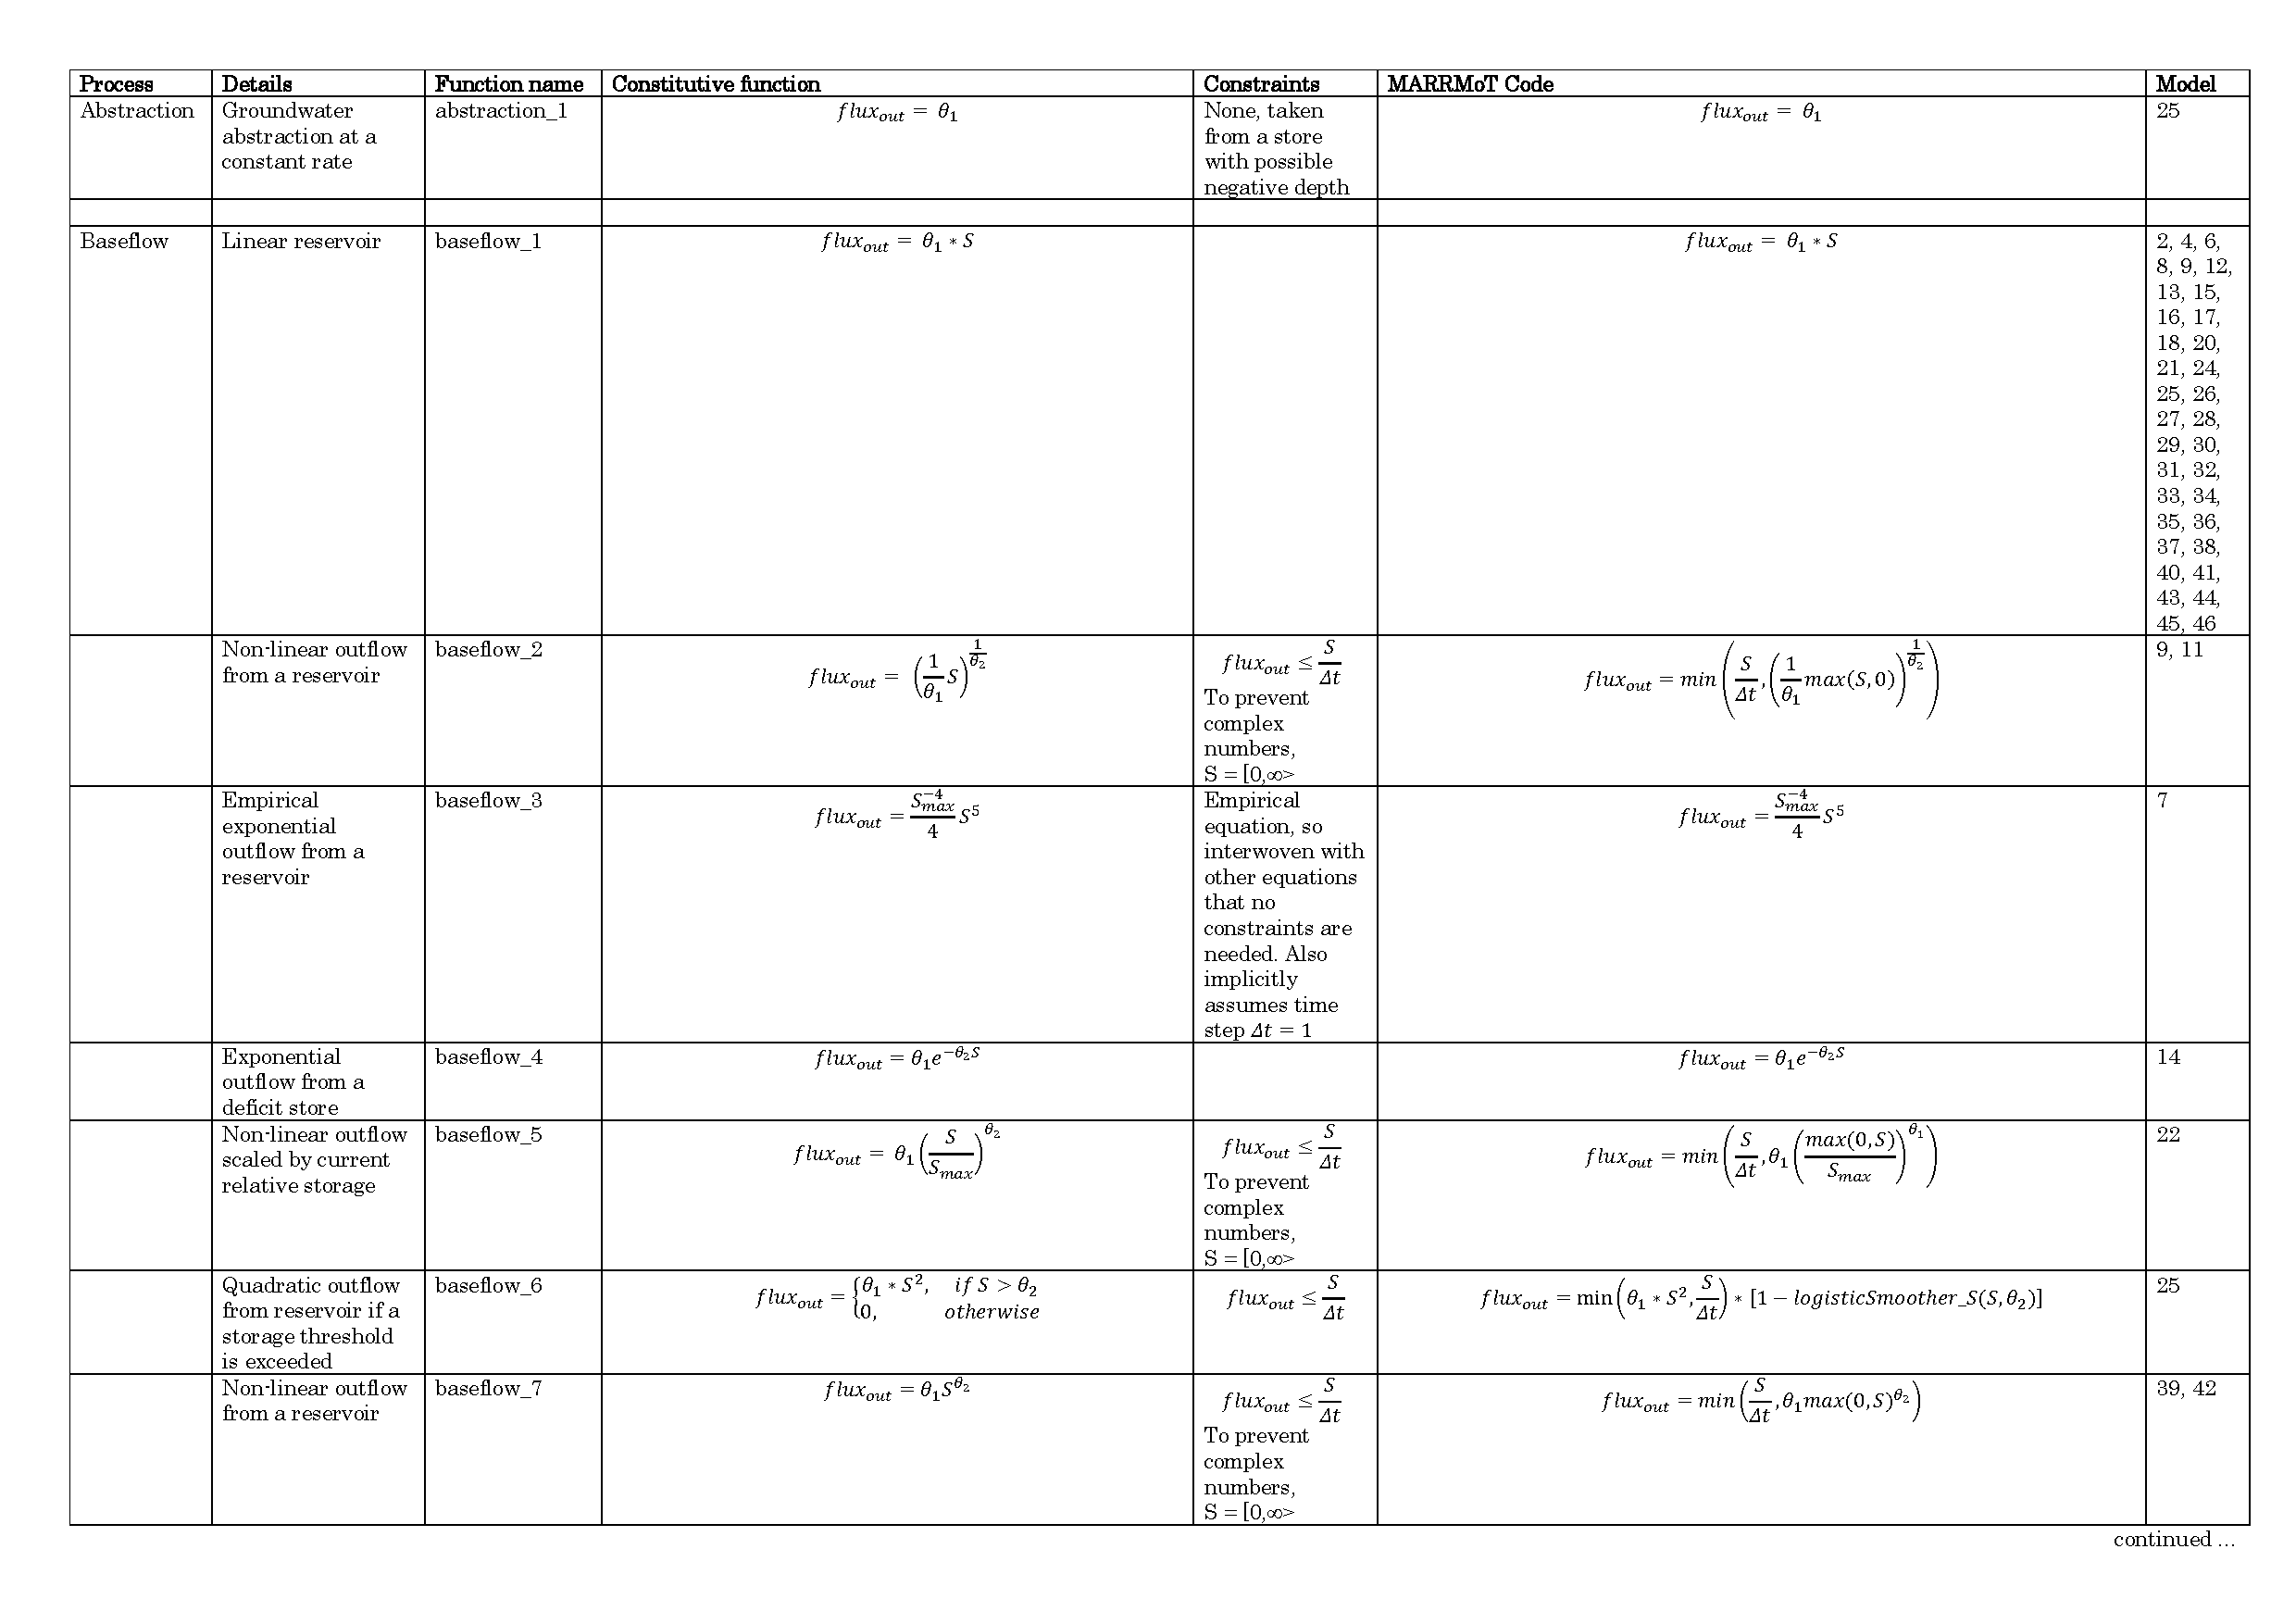
\includepdf[pages=-,landscape,pagecommand={\thispagestyle{styleLandscape}}]{sm2_fluxes.pdf}


\clearpage
\KOMAoptions{paper=A4,paper=portrait,pagesize}
\recalctypearea

























\newpage
\section{Unit Hydrographs} 		\label{sec:uhs}
This section provides details on the implementation of various Unit Hydrographs. An overview of the 8 UHs is given in Table \ref{tab:sm3_1}. Computational implementation of each UH is given in sections \ref{sec:sm3_1} to \ref{sec:sm3_8}. Unit Hydrograph files can be found in ''./MARRMoT/Models/Unit Hydrograph files/''.

% Table generated by Excel2LaTeX from sheet 'Sheet1'
\begin{table}[ht!]
  \centering
  \caption{Overview of Unit Hydrograph schemes implemented in MARRMoT}
\hspace*{-5em}    
\begin{tabular}{rp{10.57em}lrl}
    \toprule
    \multicolumn{1}{p{6.215em}}{\textbf{File name}} & \textbf{Inputs} & \multicolumn{1}{p{8.645em}}{\textbf{Diagram}} & \multicolumn{1}{p{8.43em}}{\textbf{Description }} & \multicolumn{1}{p{6.07em}}{\textbf{In model ...}} \\
    \midrule
    \multicolumn{1}{p{6.215em}}{uh\_1\_half} & 1: amount to be routed & \multirow{3}[1]{*}{ \begin{minipage}{3cm} 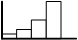
\includegraphics[height=1.3cm]{./SM3/uh1} \end{minipage}} & \multicolumn{1}{l}{Exponentially} & 7 \\
          & 2: time base &       & \multicolumn{1}{l}{increasing} &  \\
          & 3: $\Delta$t &       & \multicolumn{1}{l}{scheme} &  \\
          & \multicolumn{1}{l}{} &       &       &  \\
    \multicolumn{1}{p{6.215em}}{uh\_2\_full} & 1: amount to be routed & \multirow{3}[0]{*}{ \begin{minipage}{3cm} 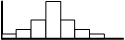
\includegraphics[height=1.3cm]{./SM3/uh2} \end{minipage} } & \multicolumn{1}{p{8.43em}}{Exponential} & 7 \\
          & 2: time base (doubled inside the function) &       & \multicolumn{1}{p{8.43em}}{triangular scheme} &  \\
          & 3: $\Delta$t &       &       &  \\
          & \multicolumn{1}{l}{} &       &       &  \\
    \multicolumn{1}{p{6.215em}}{uh\_3\_half} & 1: amount to be routed & \multirow{3}[0]{*}{ \begin{minipage}{3cm} \includegraphics[height=1.3cm]{./SM3/uh3} \end{minipage} } & \multicolumn{1}{p{8.43em}}{Triangular scheme:} & \multicolumn{1}{p{6.07em}}{13, 15, 21, 26} \\
          & 2: time base &       & \multicolumn{1}{p{8.43em}}{linearly increasing} & 34 \\
          & 3: $\Delta$t &       &       &  \\
          & \multicolumn{1}{l}{} &       &       &  \\
    \multicolumn{1}{p{6.215em}}{uh\_4\_full} & 1: amount to be routed & \multirow{3}[0]{*}{ \begin{minipage}{3cm} \includegraphics[height=1.3cm]{./SM3/uh4} \end{minipage} } & \multicolumn{1}{p{8.43em}}{Triangular scheme:} & \multicolumn{1}{p{6.07em}}{0 (template), } \\
          & 2: time base &       & \multicolumn{1}{p{8.43em}}{linearly increasing} & \multicolumn{1}{p{6.07em}}{16, 37, } \\
          & 3: $\Delta$t &       & \multicolumn{1}{p{8.43em}}{and decreasing} & \multicolumn{1}{p{6.07em}}{nn (example)} \\
          & \multicolumn{1}{l}{} &       &       &  \\
    \multicolumn{1}{p{6.215em}}{uh\_5\_half} & 1: amount to be routed & \multirow{3}[0]{*}{ \begin{minipage}{3cm} \includegraphics[height=1.3cm]{./SM3/uh5} \end{minipage} } & \multicolumn{1}{p{8.43em}}{Exponentially} & 5 \\
          & 2: time base &       & \multicolumn{1}{p{8.43em}}{decreasing} &  \\
          & 3: $\Delta$t &       & \multicolumn{1}{p{8.43em}}{scheme} &  \\
          & \multicolumn{1}{l}{} &       &       &  \\
    \multicolumn{1}{p{6.215em}}{uh\_6\_gamma} & 1: amount to be routed & \multirow{4}[0]{*}{ \begin{minipage}{3cm} \includegraphics[height=1.3cm]{./SM3/uh6} \end{minipage} } & \multicolumn{1}{p{8.43em}}{Gamma function-} & 40 \\
          & 2: gamma parameter [-] &       & \multicolumn{1}{p{8.43em}}{based} &  \\
          & 3: time for flow to reduce by factor e [d] &       &       &  \\
          & 4: length of time series &       &       &  \\
          & \multicolumn{1}{l}{} &       &       &  \\
    \multicolumn{1}{p{6.215em}}{uh\_7\_uniform} & 1: amount to be routed & \multirow{3}[1]{*}{ \begin{minipage}{3cm} \includegraphics[height=1.3cm]{./SM3/uh7} \end{minipage} } & \multicolumn{1}{p{8.43em}}{Uniform} & 39 \\
          & 2: time base &       & \multicolumn{1}{p{8.43em}}{distribution} &  \\
          & 3: $\Delta$t  &       &       &  \\
          & \multicolumn{1}{l}{} &       &       &  \\

\multicolumn{1}{p{6.215em}}{uh\_8\_delay} & 1: amount to be delayed & \multirow{3}[1]{*}{ \begin{minipage}{3cm} \includegraphics[height=1.3cm]{./SM3/uh8} \end{minipage} } & \multicolumn{1}{p{8.43em}}{Pure time} & 5 \\
          & 2: time delay &       & \multicolumn{1}{p{8.43em}}{delay} &  \\
          & 3: $\Delta$t  &       &       &  \\

    \bottomrule
    \end{tabular}%
  \label{tab:sm3_1}%
\end{table}%

%UH1
\newpage
\subsection{Code: uh\_1\_half} \label{sec:sm3_1}
This section provides the computational implementation of a unit hydrograph with an increasing exponential distribution of flows. \\

\begin{tabular}{ll}
	File location & 	./MARRMoT/Models/Unit Hydrograph files/uh\_1\_half \\
	References & 	E.g. GR4J \citep{Perrin2003} \\
\end{tabular}

\bigskip
\lstinputlisting[style=Matlab-editor]{"C:/Users/wk14463/Google Drive/PhD/Calculations/10. MARRMoT - review/Models/Unit hydrograph files/uh_1_half.m"}

%UH2
\subsection{Code: uh\_2\_full} \label{sec:sm3_2}
This section provides the computational implementation of a unit hydrograph with an exponential triangular distribution of flows. \\

\begin{tabular}{ll}
	File location & 	./MARRMoT/Models/Unit Hydrograph files/uh\_2\_full \\
	References & 	E.g. GR4J \citep{Perrin2003} \\
\end{tabular}

\bigskip
\lstinputlisting[style=Matlab-editor]{"C:/Users/wk14463/Google Drive/PhD/Calculations/10. MARRMoT - review/Models/Unit hydrograph files/uh_2_full.m"}

%UH3
\subsection{Code: uh\_3\_half} \label{sec:sm3_3}
This section provides the computational implementation of a unit hydrograph with an linearly increasing distribution of flows. \\

\begin{tabular}{ll}
	File location & 	./MARRMoT/Models/Unit Hydrograph files/uh\_3\_half \\
	References & 	E.g. FLEX-Topo \citep{Savenije2010}
\end{tabular}

\bigskip
\lstinputlisting[style=Matlab-editor]{"C:/Users/wk14463/Google Drive/PhD/Calculations/10. MARRMoT - review/Models/Unit hydrograph files/uh_3_half.m"}

%UH4
\subsection{Code: uh\_4\_full} \label{sec:sm3_4}
This section provides the computational implementation of a unit hydrograph with an linear triangular distribution of flows. \\

\begin{tabular}{ll}
	File location & 	./MARRMoT/Models/Unit Hydrograph files/uh\_4\_full \\
	References & 	E.g. HBV-96 \citep{Lindstrom1997} \\
\end{tabular}

\bigskip
\lstinputlisting[style=Matlab-editor]{"C:/Users/wk14463/Google Drive/PhD/Calculations/10. MARRMoT - review/Models/Unit hydrograph files/uh_4_full.m"}

%UH5
\subsection{Code: uh\_5\_half} \label{sec:sm3_5}
This section provides the computational implementation of a unit hydrograph with an decreasing exponential distribution of flows. \\

\begin{tabular}{ll}
	File location & 	./MARRMoT/Models/Unit Hydrograph files/uh\_5\_half \\
	References & 	E.g. IHACRES \citep{Littlewood1997,Croke2004} \\
\end{tabular}

\bigskip
\lstinputlisting[style=Matlab-editor]{"C:/Users/wk14463/Google Drive/PhD/Calculations/10. MARRMoT - review/Models/Unit hydrograph files/uh_1_half.m"}

%UH6
\subsection{Code: uh\_6\_gamma} \label{sec:sm3_6}
This section provides the computational implementation of a unit hydrograph with a gamma distribution of flows. \\

\begin{tabular}{ll}
	File location & 	./MARRMoT/Models/Unit Hydrograph files/uh\_6\_gamma \\
	References & 	E.g. SMAR \citep{OConnell1970,Tan1996} \\
\end{tabular}

\bigskip
\lstinputlisting[style=Matlab-editor]{"C:/Users/wk14463/Google Drive/PhD/Calculations/10. MARRMoT - review/Models/Unit hydrograph files/uh_6_gamma.m"}

%UH7
\subsection{Code: uh\_7\_uniform} \label{sec:sm3_7}
This section provides the computational implementation of a unit hydrograph with a uniform distribution of flows. \\

\begin{tabular}{ll}
	File location & 	./MARRMoT/Models/Unit Hydrograph files/uh\_7\_uniform \\
	References & 	E.g. MCRM \citep{Moore2001a,Moore2001} \\
\end{tabular}

\bigskip
\lstinputlisting[style=Matlab-editor]{"C:/Users/wk14463/Google Drive/PhD/Calculations/10. MARRMoT - review/Models/Unit hydrograph files/uh_7_uniform.m"}

%UH8
\subsection{Code: uh\_8\_delay} \label{sec:sm3_8}
This section provides the computational implementation of a unit hydrograph that delays flow without transforming it. \\

\begin{tabular}{ll}
	File location & 	./MARRMoT/Models/Unit Hydrograph files/uh\_8\_delay \\
	References & 	E.g. IHACRES \citep{Littlewood1997,Croke2004} \\
\end{tabular}

\bigskip
\lstinputlisting[style=Matlab-editor]{"C:/Users/wk14463/Google Drive/PhD/Calculations/10. MARRMoT - review/Models/Unit hydrograph files/uh_8_delay.m"}



\newpage
\section{Parameter ranges} 	\label{sec:pars}
Each model function in MARRMoT is accompanied by a file that specifies suitable sampling ranges for each parameter used in the model, that could be applied if the user chooses to pair MARRMoT with a calibration or parameter sampling procedure. This section gives the reasoning behind our choices of parameter ranges used within MARRMoT.

\subsection{Model-specific ranges versus generalised process-specific ranges}
There are two different approaches to determining parameter ranges for model calibration or parameter sampling studies: (1) make a choice for appropriate parameter ranges per model, based on previous applications of the model, or (2) try to make consistent choices for all models based on literature (e.g. ensure that all 'slow' linear reservoirs, regardless of which model they are part of, have the same limits for the drainage time scale parameter). 
Generalization of parameter ranges across models is difficult because models use different flux formulations and thus different parameter values might be appropriate, even if the fluxes are intended to represent the same hydrologic process. 
On the other hand, using model-specific parameter ranges based on earlier studies might limit a model's potential. 
Especially if the model has only been applied to a small number of places, published 'appropriate' parameter ranges might also reflect the climate or catchment characteristics of the few study catchments the model has been applied to. 
MARRMoT is intended as a model comparison framework. 
We thus attempt to generalize parameter ranges across all models in the framework, to facilitate fair comparison of different models. 
We try to err on the side of caution and intentionally set these ranges wide. 
Table \ref{tab:sm4_1} shows the parameter ranges used in MARRMoT and specifies in which model(s) each parameter range is used.

% BIIIIIIG table

% switch to landscape
\clearpage
\KOMAoptions{paper=A4,paper=landscape,pagesize}
\recalctypearea

% reset pagestyle to have proper footers
\pagestyle{styleLandscapeA4}

%\afterpage{\clearpage}
%\begin{landscape}
%\pagestyle{empty}
%\centering

\setlength\LTleft{-2in}
\setlength\LTright{-2in}

\begin{longtable}{p{11.215em}ccccp{13em}p{13em}l}
\caption{Parameter ranges used in MARRMoT\label{tab:sm4_1}}\\
\toprule
\textbf{Description} & \multicolumn{1}{p{3.57em}}{\textbf{Min(lit)}} & \multicolumn{1}{p{3.785em}}{\textbf{Max(lit) }} & \multicolumn{1}{p{4.645em}}{\textbf{Min(used) }} & \multicolumn{1}{p{4.785em}}{\textbf{Max(used) }} & \textbf{Reference(s)} & \textbf{Notes} & \multicolumn{1}{p{10em}}{\textbf{Model}} \\
\midrule
\endfirsthead
\multicolumn{8}{@{}l}{\ldots continued}\\
\toprule
\textbf{Description} & \multicolumn{1}{p{3.57em}}{\textbf{Min(lit)}} & \multicolumn{1}{p{3.785em}}{\textbf{Max(lit) }} & \multicolumn{1}{p{4.645em}}{\textbf{Min(used) }} & \multicolumn{1}{p{4.785em}}{\textbf{Max(used) }} & \textbf{Reference(s)} & \textbf{Notes} & \multicolumn{1}{p{10em}}{\textbf{Model}} \\
\midrule
\endhead % all the lines above this will be repeated on every page

\bottomrule
\multicolumn{8}{r@{}}{continued \ldots}\\
\endfoot
\bottomrule
\endlastfoot

% Snow
\textbf{Snow} &       &       &       &       & \multicolumn{1}{l}{} & \multicolumn{1}{l}{} &  \\
    Threshold temperature for snowfall (and melt, if not specified otherwise) $[^oC]$ & \multicolumn{1}{p{3.57em}}{Table \ref{tab:sm4_ts}} & \multicolumn{1}{p{3.785em}}{Table \ref{tab:sm4_ts}} & -3    & 5     & \cite{Kienzle2008,Kollat2012} & \multicolumn{1}{l}{} & \multicolumn{1}{p{10em}}{6, 12, 30, 31, 32, 34, 35, 37, 43, 44, 45} \\
    Threshold interval width for snowfall $[^oC]$ & 0     & 7     & 0     & 17    & \cite{Kienzle2008} & 0 is a physical limit & 37 \\
    Threshold temperature for melt $[^oC]$ &       &       & -3    & 3     & \multicolumn{1}{l}{} & Not easy to find any interval. Temperature for melt tends be treated as constant at 0 & \multicolumn{1}{p{10em}}{37, 43, 44} \\
    Degree-day-factor for snow or ice melt $[mm/^oC/d]$ & 0     & \multicolumn{1}{p{3.785em}}{Table \ref{tab:sm4_ddf}} & 0     & 20    & \multicolumn{1}{l}{} & 0 is a physical limit & \multicolumn{1}{p{10em}}{6, 12, 30, 31, 32, 34, 35, 37, 41, 43, 44, 45} \\
    Water holding content of snow pack [-] & 0     & 0.8   & 0     & 1     & \cite{Kollat2012} & [0,1] are physical limits & \multicolumn{1}{p{10em}}{37, 44} \\
    Refreezing factor of retained liquid water [-] & 0     & 1     & 0     & 1     & \multicolumn{1}{l}{} & [0,1] are physical limits & \multicolumn{1}{p{10em}}{37, 44 (given as fraction [0,1] of degree-day-factor)} \\
    Maximum melt rate due to ground-heat flux [mm/d] & 0     & 2     & 0     & 2     & \cite{Schaefli2014} & \multicolumn{1}{l}{} & 44 \\
    \multicolumn{1}{l}{} &       &       &       &       & \multicolumn{1}{l}{} & \multicolumn{1}{l}{} &  \\

\newpage

% Interception
	\textbf{Interception} &       &       &       &       & \multicolumn{1}{l}{} & \multicolumn{1}{l}{} &  \\
    Maximum store depth [mm] & 0     & \multicolumn{1}{p{3.785em}}{Table \ref{tab:sm4_int}} & 0     & 5     & \cite{Chiew1994,Gerrits2010} & 0 is a physical limit. \cite{Gerrits2010} (table 1.1) reports 3.8mm as maximum value used out of 15 studies. \cite{Chiew1994} (table 3) report 5.6mm as a maximum value for 28 catchments  & \multicolumn{1}{p{10em}}{2, 13, 15, 16, 18, 22, 23, 26, 34, 36, 39, 42, 44, 45} \\
    Maximum intercepted fraction of precipitation [-] & 0     & 0.42  & 0     & 1     & \cite{Gerrits2010} & [0,1] are physical limits. \cite{Gerrits2010} (table 1.1) reports 42\% as maximum intercepted fraction out of 15 studies & \multicolumn{1}{p{10em}}{8, 23, 32, 35, 45} \\
    Seasonal variation in LAI as fraction of mean [-] &       &       & 0     & 1     & \multicolumn{1}{l}{} & 0 is a physical limit & 22 \\
    Timing of maximum Leaf Area Index [d] &       &       & 1     & 365   & \multicolumn{1}{l}{} & Refers to days in a normal calendar year & \multicolumn{1}{p{10em}}{22, 32, 35} \\
    \multicolumn{1}{l}{} &       &       &       &       & \multicolumn{1}{l}{} & \multicolumn{1}{l}{} &  \\

% Depression
\textbf{Surface depression} &       &       &       &       & \multicolumn{1}{l}{} & \multicolumn{1}{l}{} &  \\
    Maximum surface area contributing to store [-] & 0     & 1     & 0     & 1     & \multicolumn{1}{l}{} & [0,1] are physical limits & \multicolumn{1}{p{10em}}{36, 45} \\
    Maximum store depth [mm] & 0     & \multicolumn{1}{p{3.785em}}{Table \ref{tab:sm4_dep}} & 0     & 50    & \cite{Chiew1994} & 0 is physical limit. 50 is recommended in \cite{Chiew1994} & \multicolumn{1}{p{10em}}{36, 45} \\
    Filling parameter [-] & 1     & 1     & 0.99  & 1     & \cite{Chiew1990,Porter1971} & Controls the exponential rate of depression store inflow flux but is usually set at 1 because no studies are available that can be used to set plausible ranges  & 36 \\
    \multicolumn{1}{l}{} &       &       &       &       & \multicolumn{1}{l}{} & \multicolumn{1}{l}{} &  \\

% Infiltration
\textbf{Infiltration} &       &       &       &       & \multicolumn{1}{l}{} & \multicolumn{1}{l}{} &  \\
    Maximum loss [mm] & 0     & 400   & 0     & 600   & \cite{Chiew2002} & Fig 11.11a shows calibrated parameter values for 339 catchments. Pattern indicates that limit was set at 400 & \multicolumn{1}{p{10em}}{18, 36} \\
    Loss exponent [-] & 0     & 12    & 0     & 15    & \cite{Chiew2002} & Fig 11.11a shows calibrated parameter values for 339 catchments. Pattern indicates that limit was set at 10 & \multicolumn{1}{p{10em}}{18, 36} \\
    Maximum infiltration rate [mm/d] & \multicolumn{1}{p{3.57em}}{Table \ref{tab:sm4_inf}} & \multicolumn{1}{p{3.785em}}{Table \ref{tab:sm4_inf}} & 0     & 200   & \multicolumn{1}{l}{} & Infiltration rates can be very high. However, to have a practical effect on modelling, (i.e. generate infiltration excess flow), Inf\_rate < P(t). In the context of a follow-up study, Inf\_rate is capped at 200mm/d because the maximum daily P in the study area is 200mm/d. & \multicolumn{1}{p{10em}}{15, 20, 23, 40, 44} \\
    Infiltration decline non-linearity parameter [-] &       &       & 0     & 5     & \cite{Sivapalan1996a} & Very difficult to find information for (original paper mentions nothing) & \multicolumn{1}{p{10em}}{23, 43} \\
    \multicolumn{1}{l}{} &       &       &       &       & \multicolumn{1}{l}{} & \multicolumn{1}{l}{} &  \\

% Evaporation
\textbf{Evaporation} &       &       &       &       & \multicolumn{1}{l}{} & \multicolumn{1}{l}{} &  \\
    Plant-controlled maximum rate [mm/d] & 5     & 24.5  & 0     & 20    & \cite{Chiew1994} & Although the study reports an upper value of 24.5, the recommended range is capped at 20 (paper appendix) & \multicolumn{1}{p{10em}}{20, 36} \\
    Wilting point as fraction of Soil moisture capacity [-] & 0.1   & 0.25  & 0.05  & 0.95  & \cite{Son2007} & 0 is a physical limit but can break model equations through "divide-by-zero" errors. 1 is a physical limit & \multicolumn{1}{p{10em}}{3, 4, 8, 9, 10, 12, 14, 15, 16, 19, 20, 21, 26, 31, 32, 34, 35, 37, 44} \\
    Moisture constrained rate parameter [-] &       &       & 0     & 1     & \multicolumn{1}{l}{} & [0,1] are physical limits & 15 \\
    Forest fraction for separate soil/vegetation evap [-] & 0     & 1     & 0.05  & 0.95  & \multicolumn{1}{l}{} & [0,1] are physical limits, but using these limits can result in divide-by-zero-errors in certain fluxes & \multicolumn{1}{p{10em}}{3, 4, 8, 9, 16} \\
    Phenology: minimum temperature where transpiration stops $[^oC]$ & -5    & -5    & 0     & -10   & \cite{Ye2012} & \multicolumn{1}{l}{} & 35 \\
    Phenology: maximum temperature above which transpiration fully utilizes Ep $[^oC]$ & 10    & 10    & 1     & 20    & \cite{Ye2012} & The setup of minimum and maximum temperature used in Ye et al. (2012) is here changed to a minimum temperature + temperature range (Tmax = Tmin + Trange) to avoid overlap in parameter values & 35 \\
    Evaporation reduction with depth coefficient [-] & 0.083 & 1     & 0     & 1     & \cite{PENMAN1950,Tan1996} & [0,1] are physical limits & \multicolumn{1}{p{10em}}{17, 23, 25, 40} \\
    Shape parameter for evaporation reduction in a deficit store [-] &       &       & 0     & 1     & \cite{Moore2001} & This uses a sigmoid function to determine a fraction of Ep to evaporate. Values >1 make the transition very steep & 39 \\
    Evaporation non-linearity coefficient [-] &       &       & 0     & 10    & \cite{Sivapalan1996a} & Very difficult to find information for. Assumption made to be in line with other non-linearity coefficients. & \multicolumn{1}{p{10em}}{23, 43} \\
    \multicolumn{1}{l}{} &       &       &       &       & \multicolumn{1}{l}{} & \multicolumn{1}{l}{} &  \\

% Soil moisture
\textbf{Soil moisture} &       &       &       &       & \multicolumn{1}{l}{} & \multicolumn{1}{l}{} &  \\
    Maximum store depth [mm] & 1     & \multicolumn{1}{p{3.785em}}{Table \ref{tab:sm4_sm}} & 1     & 2000  & \multicolumn{1}{l}{} & 0 is a physical limit & \multicolumn{1}{p{10em}}{1, 2, 3, 4, 5, 6, 7, 8, 9, 10, 11, 12, 13, 14, 15, 16, 17, 18, 19, 20, 21, 22, 23, 24, 26, 27, 28, 29, 30, 31, 32, 33, 34, 35, 36, 37, 38, 39, 40, 41, 42, 43, 44, 45, 46} \\
    Capillary rise [mm/d] & 0     & \multicolumn{1}{p{3.785em}}{Table \ref{tab:sm4_cap}} & 0     & 4     & \multicolumn{1}{l}{} & 0 is a physical limit & \multicolumn{1}{p{10em}}{13, 15, 37, 38} \\
    \multicolumn{1}{l}{} &       &       &       &       & \multicolumn{1}{l}{} & SMHI gives a default value of 1 mm/d for use with HBV. We use a wider range here &  \\
    Percolation rate [mm/d] & 0     & \multicolumn{1}{p{3.785em}}{Table \ref{tab:sm4_perc}} & 0     & 20    & \cite{Bethune2008} & Some modelling studies report very large percolation rates (100 mm/d). \cite{Bethune2008} report ~11mm/d from field observations.  & \multicolumn{1}{p{10em}}{21, 26, 34, 37, 39, 44, 45} \\
    Percolation fraction [-] & 0.013 & 0.533 & 0     & 1     & \cite{Ye2012} (Table 1) & [0,1] are physical limits & \multicolumn{1}{p{10em}}{14, 22, 23, 24, 27, 30, 31, 32, 35, 45} \\
    Recharge nonlinearity [-] & 0     & 7     & 0     & 10    & \cite{Kollat2012} & Also seen as a soil depth distribution & \multicolumn{1}{p{10em}}{5, 22, 33, 37} \\
    Soil depth distribution [-] & 0     & \multicolumn{1}{p{3.785em}}{Table \ref{tab:sm4_soilnl}} & 0     & 10    & \multicolumn{1}{l}{} & For cases where the soil depth is not considered constant. Most studies limit this to 0-2.5 but this seems based on a single source \citep{Wagener2004} which is UK only. Thus we use a wider range here & \multicolumn{1}{p{10em}}{2, 13, 15, 21, 22, 26, 28, 29, 34} \\
    Porosity [-] & 0.35  & 0.5   & 0.05  & 0.95  & \cite{Son2007} & [0,1] are theoretical physical limits, but no (0) porosity and full (1) porosity are not sensible: there would be no soil moisture or soil respectively & \multicolumn{1}{p{10em}}{10, 19} \\
    Gamma distribution for topographic indices - phi [-] & 0.4   & 3.5   & 0.1   & 5     & \cite{Clark2008a} & \multicolumn{1}{l}{} & 14 \\
    Gamma distribution for topographic indices - chi [-] & 2     & 5     & 1     & 7.5   & \cite{Clark2008a} & \multicolumn{1}{l}{} & 14 \\
    Fraction area with permeable soils [-] &       &       & 0     & 1     & \cite{Crooks2007} & [0,1] are physical limits & 46 \\
    Fraction area with semi-permeable soils [-] &       &       & 0     & 1     & \cite{Crooks2007} & [0,1] are physical limits & 46 \\
    Fraction area with impermeable soils [-] &       &       & 0     & 1     & \cite{Crooks2007} & [0,1] are physical limits & 46 \\
    Variable contributing area scaling [-]  &       &       & 0     & 5     & \cite{Sivapalan1996a} & Very difficult to find information about this. Assumption made  & 23 \\
    Variable contributing area non-linearity [-] &       &       &       &       & \cite{Sivapalan1996a} & See: \textbf{Soil depth distribution} above & 23 \\
    Fraction of D50 that is D16 [-] &       &       & 0.01  & 0.99  & \multicolumn{1}{l}{} & Note: re-writing of D16 parameter in \cite{Fukushima1988} & 42 \\
    Variable contributing area equation inflection point [-] & -0.5  & 0.5   & -0.5  & 0.5   & \cite{Jayawardena2000} & \multicolumn{1}{l}{} & 28 \\
    \multicolumn{1}{l}{} &       &       &       &       & \multicolumn{1}{l}{} & \multicolumn{1}{l}{} &  \\

% Groundwater
\textbf{Groundwater} &       &       &       &       & \multicolumn{1}{l}{} & \multicolumn{1}{l}{} &  \\
    Leakage coefficient [-] & 0.07  & 0.13  & 0     & 0.5   & \cite{Chiew1994} & 0 is physical limit. 0.5 is recommended in the paper's appendix & 36 \\
    Leakage rate [mm/d] &       &       &       &       & \multicolumn{1}{l}{} & See: \textbf{Percolation rate} above &  \\
    Level compared to channel level [mm] & -2.8  & 3.9   & -10   & 10    & \cite{Chiew1994} & Range recommended in appendix of the paper & 36 \\
    Base flow rate at no deficit [mm/d] & 0     & 201.6 & 0.1   & 200   & \cite{Beven1997} & Based on Table 2 \citep{Beven1997} & \multicolumn{1}{p{10em}}{14, 23} \\
    Baseflow deficit scaling parameter [-] &       &       & 0     & 1     & \multicolumn{1}{l}{} & [0,1] are physical limits & \multicolumn{1}{p{10em}}{14, 23} \\
    \multicolumn{1}{l}{} &       &       &       &       & \multicolumn{1}{l}{} & \multicolumn{1}{l}{} &  \\

% Flow distribution
\textbf{Flow distribution} &       &       &       &       & \multicolumn{1}{l}{} & \multicolumn{1}{l}{} &  \\
    Interflow and saturation excess [-] & 0     & 1     & 0     & 1     & \multicolumn{1}{l}{} & [0,1] are physical limits & \multicolumn{1}{p{10em}}{18, 36} \\
    Preferential recharge [-]& 0     & 2     & 0     & 1     & \cite{Chiew1994} & 0 is a physical limit. Later paper sets max limit to 1 & \multicolumn{1}{p{10em}}{18, 25, 36, 46} \\
    Surface/groundwater division  [-]&       &       & 0     & 1     & \multicolumn{1}{l}{} & [0,1] are physical limits & \multicolumn{1}{p{10em}}{13, 17, 33} \\
    Fast and slow flow [-]& 0     & 1     & 0     & 1     & \multicolumn{1}{l}{} & [0,1] are physical limits & \multicolumn{1}{p{10em}}{21, 26, 29, 34, 46} \\
    Groundwater recharge and interflow [-]& 0.05  & 0.3   & 0     & 1     & \cite{Son2007} & [0,1] are physical limits & \multicolumn{1}{p{10em}}{10, 11, 20, 40} \\
    Infiltration and direct runoff [-] & 0.161 & 0.422 & 0     & 1     & \cite{Tan1996} & [0,1] are physical limits & 40 \\
    Impervious and infiltration area [-]&       &       & 0     & 1     & \multicolumn{1}{l}{} & [0,1] are physical limits & \multicolumn{1}{p{10em}}{28, 33, 45} \\
    Contributing area to overland flow [-]&       &       & 0     & 1     & \multicolumn{1}{l}{} & [0,1] are physical limits & \multicolumn{1}{p{10em}}{39, 45} \\
    Tension water and free water [-]&       &       & 0     & 1     & \multicolumn{1}{l}{} & [0,1] are physical limits & 33 \\
    Threshold for overland flow generation [-] & 0     & \multicolumn{1}{p{3.785em}}{<1} & 0     & 0.99  & \cite{Nielsen1973} & [0,1] are physical limits & 41 \\
    Threshold for overland flow generation [-]& 0     & \multicolumn{1}{p{3.785em}}{<1} & 0     & 0.99  & \cite{Nielsen1973} & [0,1] are physical limits & 41 \\
    Channel and land division [-]&       &       & 0     & 1     & \multicolumn{1}{l}{} & [0,1] are physical limits & 42 \\
    Throughfall/stem flow division [-]&       &       & 0     & 1     & \multicolumn{1}{l}{} & [0,1] are physical limits & 42 \\
    Glacier/non-glacier precipitation [-]&       &       & 0     & 1     & \multicolumn{1}{l}{} & [0,1] are physical limits & 43 \\
    \multicolumn{1}{l}{} &       &       &       &       & \multicolumn{1}{l}{} & \multicolumn{1}{l}{} &  \\

% Flow scale and shape
\textbf{Flow time scale and shape} &       &       &       &       & \multicolumn{1}{l}{} & \multicolumn{1}{l}{} &  \\
    Fast reservoir time scale [d-1] & 0.05  & \multicolumn{1}{p{3.785em}}{Table \ref{tab:sm4_kf}} & 0     & 1     & \multicolumn{1}{l}{} & 0 is a physical limit & \multicolumn{1}{p{10em}}{12, 21, 24, 26, 28, 29, 30, 31, 32, 33, 34, 35, 37, 39, 41, 42, 43, 44, 46} \\
    Slow reservoir time scale [d-1] & 0.01  & \multicolumn{1}{p{3.785em}}{Table \ref{tab:sm4_ks}} & 0     & 1     & \multicolumn{1}{l}{} & 0 is a physical limit & \multicolumn{1}{p{10em}}{2, 3, 4, 6, 8, 10, 13, 15, 16, 17, 18, 19, 20, 21, 22, 24, 25, 26, 28, 29, 30, 31, 32, 33, 34, 35, 37, 39, 40, 41, 42, 43, 44, 46} \\
    Flow non-linearity S\^x [-] & 0     & \multicolumn{1}{p{3.785em}}{Table \ref{tab:sm4_flownl}} & 1     & 5     & \multicolumn{1}{l}{} & \multicolumn{1}{l}{} & \multicolumn{1}{p{10em}}{4, 9, 10, 11, 16, 19, 22, 23, 37, 39, 42, 44, 45} \\
    Flow reduction (S/X) [mm] & 5     & 40    & 1     & 50    & \cite{Son2007} & \multicolumn{1}{l}{} & 9 \\
    Exponential shape parameter [mm-1] &       &       & 0     & 2     & \cite{Moore2001} & Very difficult to find documentation for & 39 \\
    \multicolumn{1}{l}{} &       &       &       &       & \multicolumn{1}{l}{} & \multicolumn{1}{l}{} &  \\
    \textbf{Routing } &       &       &       &       & \multicolumn{1}{l}{} & \multicolumn{1}{l}{} &  \\
    Routing delay to fast flow [d] & 0     & 1     & 1     & 5     & \cite{Fenicia2008} & \multicolumn{1}{l}{} & \multicolumn{1}{p{10em}}{21, 26, 34} \\
    Routing delay to slow flow [d] & 0     & 8     & 1     & 15    & \multicolumn{1}{l}{} & \multicolumn{1}{l}{} & \multicolumn{1}{p{10em}}{7, 21, 26, 34} \\
    Routing delay [d] & 1     & \multicolumn{1}{p{3.785em}}{Table \ref{tab:sm4_rout}} & 1     & 120   & \cite{Kollat2012} & 1 is the limit (water shouldn't speed up). 120 because it seems very high & \multicolumn{1}{p{10em}}{13, 15, 16, 21, 37, 39, 40} \\
    IHACRES routing delay [d] & 0.8 & 641 & 1 & 700 & \cite{Sefton1998} & These Unit Hydrograps are intended to represent linear reservoirs. Large values chosen for consistency with other models that rely on linear reservoirs & 5 \\
    Pure delay (no transformation) [d] & 1     & \multicolumn{1}{p{3.785em}}{} & 0     & 119   & See \textbf{Routing delay} & Alternative formulation of the information in \textbf{Routing delay} for a function that does not transform a flux \emph{over} several time steps but delays the flux \emph{by} a certain time & \multicolumn{1}{p{10em}}{5} \\
%    Pure delay (no transformation) [d] &       & \multicolumn{1}{p{3.785em}}{ } & 1     & 120   & \cite{Kollat2012} & 1 is the limit (water shouldn't speed up). 120 because it seems very high & \multicolumn{1}{p{10em}}{13, 15, 16, 21, 37, 39, 40} \\
    Routing store depth [mm] & 1     & 300   & 1     & 300   & \cite{Perrin2003} & \multicolumn{1}{l}{} & \multicolumn{1}{p{10em}}{7, 20, 39, 45} \\
    Gamma function, number of Nash cascade reservoirs [-] & 0.75  & 9.79  & 1     & 10    & \cite{Tan1996} & 0 would mean no routing, so slightly above that & 40 \\
    \multicolumn{1}{l}{} &       &       &       &       & \multicolumn{1}{l}{} & \multicolumn{1}{l}{} &  \\

% Water exchange
    \textbf{Water exchange parameters} &       &       &       &       & \multicolumn{1}{l}{} & \multicolumn{1}{l}{} &  \\
    Coefficient 1 [-]  & 0.005 & 0.54  & 0     & 1     & \cite{Chiew1994} & Although the study only reports values up to 0.54, an upper range of 1 is recommended in the study's appendix & 36 \\
    Coefficient 2 [-]  & 0.01  & 0.29  & 0     & 1     & \cite{Chiew1994} & Although the study only reports values up to 0.29, an upper range of 1 is recommended in the study's appendix & 36 \\
    Coefficient 3 [-]  & 0     & 13    & 0     & 100   & \cite{Chiew1994} & Although the study only reports values up to 13, an upper range of 100 is recommended in the study's appendix & 36 \\
    Water exchange coefficient [mm/d] & -10   & 14    & -10   & 15    & \cite{Perrin2003,Santos2017} & Parameter x2 in GR4J model & 7 \\
\end{longtable}

%\end{landscape}

% Reset page style
\clearpage
\KOMAoptions{paper=A4,paper=portrait,pagesize}
\recalctypearea
\pagestyle{fancy}

% SMALL TABLES
% Temp_snow
\begin{table}[htbp]
  \centering
  \caption[References: Threshold temperature for snowfall]{Literature-based ranges for snowmelt parameter ''threshold temperature for snowfall''}
    \begin{tabular}{lrr}
    \toprule
    \textbf{Threshold temperature for snowfall $[^oC]$} & \textbf{Min} & \textbf{Max} \\
    \midrule
    Table 2 in \cite{Seibert1997} & -2.5  & 2.5 \\
    Table 1 in \cite{Kollat2012} & -3    & 3 \\
    Table 2 in \cite{Kienzle2008} Note: always coupled with a snow interval [10,17] & 1.1   & 4.5 \\
    Table A3 in \cite{Seibert2012} & -1.5  & 2.5 \\
    \bottomrule
    \end{tabular}%
  \label{tab:sm4_ts}%
\end{table}%

% DDF
\begin{table}[htbp]
  \centering
  \caption[References: Degree-day-factor]{Literature-based ranges for snowmelt parameter ''degree-day-factor''}
    \begin{tabular}{lrr}
	\toprule
    \textbf{Degree-day factor for snowmelt $[mm/\^oC/d]$} & \textbf{Min} & \textbf{Max} \\
	\midrule
    Table 2 in \cite{Seibert1997} & 1     & 10 \\
    Table 1 in \cite{Kollat2012} & 0     & 20 \\
    Table A3 in \cite{Seibert2012} & 1     & 10 \\
	\bottomrule
    \end{tabular}%
  \label{tab:sm4_ddf}%
\end{table}%

% Interception
\begin{table}[htbp]
  \centering
  \caption[References: Interception capacity]{Literature-based ranges for interception parameter ''maximum interception capacity''}
    \begin{tabular}{lrr}
    \toprule
    \textbf{Interception bucket [mm]} & \textbf{Min} & \textbf{Max} \\
    \midrule
    Figure 11.11a  in \cite{Chiew2002} & 0     & 5 \\
    Table 3 in \cite{Chiew1994} & 0.5   & 5.6 \\
    Table 1.1 in \cite{Gerrits2010} & 0     & 3.8 \\
    Table 2 in \cite{Son2007} &       & 0.4 \\
    \bottomrule
    \end{tabular}%
  \label{tab:sm4_int}%
\end{table}%

% Depression
\begin{table}[htbp]
  \centering
  \caption[References: Depression capacity]{Literature-based ranges for depression parameter ''maximum depression capacity''}
    \begin{tabular}{lrr}
    \toprule
    \textbf{Depression bucket [mm]} & \textbf{Min} & \textbf{Max} \\
    \midrule
    Table 3 in \cite{Chiew1994} & 1     & 100 \\
    Table 1  in \cite{Amoah2013} & 5     & 110 \\
    \bottomrule
    \end{tabular}%
  \label{tab:sm4_dep}%
\end{table}%

% Infiltration
\begin{table}[htbp]
  \centering
  \caption[References: Infiltration rate]{Literature-based ranges for infiltration parameter ''maximum infiltration rate''}
    \begin{tabular}{lrr}
    \toprule
    \textbf{Infiltration rate } & \textbf{Min} & \textbf{Max} \\
    \midrule
    Figure 2 in \cite{Assouline2013} [mm/d] & 40    & 100 \\
    Table 3.3  in \cite{Jones1997} [mm/h] & 6     & 76 \\
    Table 3 in \cite{Cerda1996} [mm/h] & 50    & 770 \\
    \bottomrule
    \end{tabular}%
  \label{tab:sm4_inf}%
\end{table}%


% Soil moisture
\begin{table}[htbp]
  \centering
  \caption[References: Soil moisture capacity]{Literature-based ranges for soil moisture parameter ''maximum soil moisture capacity''}
    \begin{tabular}{lrr}
    \toprule
    \textbf{Soil moisture bucket [mm]} & \textbf{Min} & \textbf{Max} \\
    \midrule
    Figure 11.11b in \cite{Chiew2002} & 0     & 500 \\
    Table 3 in \cite{Chiew1994} & 65    & 400 \\
    Table 2 in \cite{Seibert1997} & 50    & 500 \\
    Table 1 in \cite{Rusli2015} & 100   & 800 \\
    Table 1 in \cite{Kollat2012} & 0     & 2000 \\
    Table A3 in \cite{Seibert2012} & 50    & 500 \\
    Table 3 in \cite{Sun2015} & 1     & 500 \\
    \bottomrule
    \end{tabular}%
  \label{tab:sm4_sm}%
\end{table}%

% Cappilary rise
\begin{table}[htbp]
  \centering
  \caption[References: Capillary rise rate]{Literature-based ranges for capillary rise parameter ''maximum capillary rise rate''}
    \begin{tabular}{lrr}
    \toprule
    \textbf{Capillary rise [mm/d]} & \textbf{Min} & \textbf{Max} \\
    \midrule
    Table 1 in \cite{Rusli2015} & 0.1   & 1 \\
    Default value in \cite{SMHI2004} & 1     & 1 \\
    Figure 3 in \cite{Bethune2008} & 0     & 0.06 \\
    \bottomrule
    \end{tabular}%
  \label{tab:sm4_cap}%
\end{table}%


% Percolation
\begin{table}[htbp]
  \centering
  \caption[References: Percolation rate]{Literature-based ranges for percolation parameter ''maximum percolation rate''}
    \begin{tabular}{lrr}
    \toprule
    \textbf{Percolation rate [mm/d]} & \textbf{Min} & \textbf{Max} \\
    \midrule
    Table 2 in \cite{Seibert1997} & 0     & 6 \\
    Table 1 in \cite{Rusli2015} & 0.1   & 5 \\
    Table 1 in \cite{Kollat2012} & 0     & 100 \\
    Figure 3 in \cite{Bethune2008} & 0     & 10.4 \\
    Table A3 in \cite{Seibert2012} & 0     & 3 \\
    \bottomrule
    \end{tabular}%
  \label{tab:sm4_perc}%
\end{table}%


% Soil depth distribution
\begin{table}[htbp]
  \centering
  \caption[References: Soil-depth distribution non-linearity]{Literature-based ranges for soil moisture parameter ''soil depth distribution non-linearity''}
    \begin{tabular}{lrr}
    \toprule
    \textbf{Soil depth distribution [-]} & \textbf{Min} & \textbf{Max} \\
    \midrule
    Table 3 in \cite{Sun2015} & 0     & 2 \\
    Figure 9 in \cite{Lamb1999} & 0     & 2.5 \\
    Table 4 in \cite{Bulygina2009} & 0     & 2.5 \\
    Figure 4.12 in \cite{Wagener2004}  & 0     & 2 \\
    Page 700 in \cite{Sivapalan1995} &       & 4.03 \\
    Figure 4 in \cite{Huang2003} Note: estimated values, ~97\% < 6 & 0     & 11.5 \\
    \bottomrule
    \end{tabular}%
  \label{tab:sm4_soilnl}%
\end{table}%

% Fast flow time
\begin{table}[htbp]
  \centering
  \caption[References: Fast flow time scale]{Literature-based ranges for flow parameter ''fast flow time scale''}
    \begin{tabular}{lrr}
    \toprule
    \textbf{Fast flow time scale $[d^{-1}]$} & \textbf{Min} & \textbf{Max} \\
    \midrule
    Table 2 in \cite{Seibert1997} & 0.05  & 0.5 \\
    Table 1 in \cite{Rusli2015} & 0.05  & 0.8 \\
    Table 1 in \cite{Kollat2012} & 0.01  & 1 \\
    Table A3 in \cite{Seibert2012} & 0.01  & 0.4 \\
    Table 3 in \cite{Sun2015} & 0.5   & 1.2 \\
    \bottomrule
    \end{tabular}%
  \label{tab:sm4_kf}%
\end{table}%

% Slow flow time
\begin{table}[htbp]
  \centering
  \caption[References: Slow flow time scale]{Literature-based ranges for flow parameter ''slow flow time scale''}
    \begin{tabular}{lrr}
    \toprule
    \textbf{Slow flow time scale $[d^{-1}]$} & \textbf{Min} & \textbf{Max} \\
    \midrule
    Figure 11.11b in \cite{Chiew2002} & 0     & 0.3 \\
    Table 2 in \cite{Son2007} & 2.40E-05 & 0.1 \\
    Table 2 in \cite{Seibert1997} & 0.001 & 0.1 \\
    Table 1 in \cite{Rusli2015} & 0.0005 & 0.1 \\
    Table 1 in \cite{Kollat2012} & 0.00005 & 0.05 \\
    Table A3 in \cite{Seibert2012} & 0.001 & 0.15 \\
    Table 3 in \cite{Sun2015} & 0.001 & 0.5 \\
    \bottomrule
    \end{tabular}%
  \label{tab:sm4_ks}%
\end{table}%

% Flow non-linearity
\begin{table}[htbp]
  \centering
  \caption[References: Flow non-linearityy]{Literature-based ranges for flow parameter ''flow non-linearity''}
    \begin{tabular}{lrr}
    \toprule
    \textbf{Flow non-linearity} & \textbf{Min} & \textbf{Max} \\
    \midrule
    Table 3 in \cite{Liden2000} – non-linearity shape $= S^{1+var}$ & 0     & 3 \\
    Table 1 in \cite{Son2007} – non-linearity shape $= S^{1/var}$ & 0.45  & 0.5 \\
    Table 3 in \cite{Jothityangkoon2001} & 0.5   & 0.5 \\
    \bottomrule
    \end{tabular}%
  \label{tab:sm4_flownl}%
\end{table}%

% Routing delay
\begin{table}[htbp]
  \centering
  \caption[References: Routing delay]{Literature-based ranges for routing parameter ''routing delay''}
    \begin{tabular}{p{0.8\linewidth}rr}
    \toprule
    \textbf{Routing delay [d]} & \textbf{Min} & \textbf{Max} \\
    \midrule
    Table 2 in \cite{Seibert1997} & 1     & 5 \\
    Table 1 in \cite{Kollat2012} & 24    & 120 \\
    Table 3 in \cite{Liden2000} & 1     & 4 \\
    Table 1 in \cite{Perrin2003} & 0.5   & 4 \\
    Table A3 in \cite{Seibert2012} & 1     & 7 \\
    Table 2 in \cite{Atkinson2003} Note: converted from a flow speed of 0.5m/s and catchment area of 47$km^2$ &       & <1 \\
    Table 3 in \cite{Goswami2010} & 12    & 36 \\
    Table 2 in \cite{Vinogradov2011} Note: approximated from flow velocities and catchment sizes & 0.01  & 4 \\
    \bottomrule
    \end{tabular}%
  \label{tab:sm4_rout}%
\end{table}%

\clearpage































%% REFERENCES
\newpage
\bibliographystyle{copernicus}
\bibliography{C:/Users/wk14463/BibTeX/library}

%% Since the Copernicus LaTeX package includes the BibTeX style file copernicus.bst,
%% authors experienced with BibTeX only have to include the following two lines:
%%
%% \bibliographystyle{copernicus}
%% \bibliography{example.bib}
%%
%% URLs and DOIs can be entered in your BibTeX file as:
%%
%% URL = {http://www.xyz.org/~jones/idx_g.htm}
%% DOI = {10.5194/xyz}


%% LITERATURE CITATIONS
%%
%% command                        & example result
%% \citet{jones90}|               & Jones et al. (1990)
%% \citep{jones90}|               & (Jones et al., 1990)
%% \citep{jones90,jones93}|       & (Jones et al., 1990, 1993)
%% \citep[p.~32]{jones90}|        & (Jones et al., 1990, p.~32)
%% \citep[e.g.,][]{jones90}|      & (e.g., Jones et al., 1990)
%% \citep[e.g.,][p.~32]{jones90}| & (e.g., Jones et al., 1990, p.~32)
%% \citeauthor{jones90}|          & Jones et al.
%% \citeyear{jones90}|            & 1990



%% FIGURES

%% When figures and tables are placed at the end of the MS (article in one-column style), please add \clearpage
%% between bibliography and first table and/or figure as well as between each table and/or figure.


%% ONE-COLUMN FIGURES

%%f
%\begin{figure}[t]
%\includegraphics[width=8.3cm]{FILE NAME}
%\caption{TEXT}
%\end{figure}
%
%%% TWO-COLUMN FIGURES
%
%%f
%\begin{figure*}[t]
%\includegraphics[width=12cm]{FILE NAME}
%\caption{TEXT}
%\end{figure*}
%
%
%%% TABLES
%%%
%%% The different columns must be seperated with a & command and should
%%% end with \\ to identify the column brake.
%
%%% ONE-COLUMN TABLE
%
%%t
%\begin{table}[t]
%\caption{TEXT}
%\begin{tabular}{column = lcr}
%\tophline
%
%\middlehline
%
%\bottomhline
%\end{tabular}
%\belowtable{} % Table Footnotes
%\end{table}
%
%%% TWO-COLUMN TABLE
%
%%t
%\begin{table*}[t]
%\caption{TEXT}
%\begin{tabular}{column = lcr}
%\tophline
%
%\middlehline
%
%\bottomhline
%\end{tabular}
%\belowtable{} % Table Footnotes
%\end{table*}
%
%%% LANDSCAPE TABLE
%
%%t
%\begin{sidewaystable*}[t]
%\caption{TEXT}
%\begin{tabular}{column = lcr}
%\tophline
%
%\middlehline
%
%\bottomhline
%\end{tabular}
%\belowtable{} % Table Footnotes
%\end{sidewaystable*}
%
%
%%% MATHEMATICAL EXPRESSIONS
%
%%% All papers typeset by Copernicus Publications follow the math typesetting regulations
%%% given by the IUPAC Green Book (IUPAC: Quantities, Units and Symbols in Physical Chemistry,
%%% 2nd Edn., Blackwell Science, available at: http://old.iupac.org/publications/books/gbook/green_book_2ed.pdf, 1993).
%%%
%%% Physical quantities/variables are typeset in italic font (t for time, T for Temperature)
%%% Indices which are not defined are typeset in italic font (x, y, z, a, b, c)
%%% Items/objects which are defined are typeset in roman font (Car A, Car B)
%%% Descriptions/specifications which are defined by itself are typeset in roman font (abs, rel, ref, tot, net, ice)
%%% Abbreviations from 2 letters are typeset in roman font (RH, LAI)
%%% Vectors are identified in bold italic font using \vec{x}
%%% Matrices are identified in bold roman font
%%% Multiplication signs are typeset using the LaTeX commands \times (for vector products, grids, and exponential notations) or \cdot
%%% The character * should not be applied as mutliplication sign
%
%
%%% EQUATIONS
%
%%% Single-row equation
%
%\begin{equation}
%
%\end{equation}
%
%%% Multiline equation
%
%\begin{align}
%& 3 + 5 = 8\\
%& 3 + 5 = 8\\
%& 3 + 5 = 8
%\end{align}
%
%
%%% MATRICES
%
%\begin{matrix}
%x & y & z\\
%x & y & z\\
%x & y & z\\
%\end{matrix}
%
%
%%% ALGORITHM
%
%\begin{algorithm}
%\caption{...}
%\label{a1}
%\begin{algorithmic}
%...
%\end{algorithmic}
%\end{algorithm}
%
%
%%% CHEMICAL FORMULAS AND REACTIONS
%
%%% For formulas embedded in the text, please use \chem{}
%
%%% The reaction environment creates labels including the letter R, i.e. (R1), (R2), etc.
%
%\begin{reaction}
%%% \rightarrow should be used for normal (one-way) chemical reactions
%%% \rightleftharpoons should be used for equilibria
%%% \leftrightarrow should be used for resonance structures
%\end{reaction}
%
%
%%% PHYSICAL UNITS
%%%
%%% Please use \unit{} and apply the exponential notation


\end{document}
